% Options for packages loaded elsewhere
\PassOptionsToPackage{unicode}{hyperref}
\PassOptionsToPackage{hyphens}{url}
%
\documentclass[
]{book}
\usepackage{lmodern}
\usepackage{amsmath}
\usepackage{ifxetex,ifluatex}
\ifnum 0\ifxetex 1\fi\ifluatex 1\fi=0 % if pdftex
  \usepackage[T1]{fontenc}
  \usepackage[utf8]{inputenc}
  \usepackage{textcomp} % provide euro and other symbols
  \usepackage{amssymb}
\else % if luatex or xetex
  \usepackage{unicode-math}
  \defaultfontfeatures{Scale=MatchLowercase}
  \defaultfontfeatures[\rmfamily]{Ligatures=TeX,Scale=1}
\fi
% Use upquote if available, for straight quotes in verbatim environments
\IfFileExists{upquote.sty}{\usepackage{upquote}}{}
\IfFileExists{microtype.sty}{% use microtype if available
  \usepackage[]{microtype}
  \UseMicrotypeSet[protrusion]{basicmath} % disable protrusion for tt fonts
}{}
\makeatletter
\@ifundefined{KOMAClassName}{% if non-KOMA class
  \IfFileExists{parskip.sty}{%
    \usepackage{parskip}
  }{% else
    \setlength{\parindent}{0pt}
    \setlength{\parskip}{6pt plus 2pt minus 1pt}}
}{% if KOMA class
  \KOMAoptions{parskip=half}}
\makeatother
\usepackage{xcolor}
\IfFileExists{xurl.sty}{\usepackage{xurl}}{} % add URL line breaks if available
\IfFileExists{bookmark.sty}{\usepackage{bookmark}}{\usepackage{hyperref}}
\hypersetup{
  pdftitle={CRIM20452 Modelling Criminological Data},
  pdfauthor={Laura Bui \& Reka Solymosi},
  hidelinks,
  pdfcreator={LaTeX via pandoc}}
\urlstyle{same} % disable monospaced font for URLs
\usepackage{color}
\usepackage{fancyvrb}
\newcommand{\VerbBar}{|}
\newcommand{\VERB}{\Verb[commandchars=\\\{\}]}
\DefineVerbatimEnvironment{Highlighting}{Verbatim}{commandchars=\\\{\}}
% Add ',fontsize=\small' for more characters per line
\usepackage{framed}
\definecolor{shadecolor}{RGB}{248,248,248}
\newenvironment{Shaded}{\begin{snugshade}}{\end{snugshade}}
\newcommand{\AlertTok}[1]{\textcolor[rgb]{0.94,0.16,0.16}{#1}}
\newcommand{\AnnotationTok}[1]{\textcolor[rgb]{0.56,0.35,0.01}{\textbf{\textit{#1}}}}
\newcommand{\AttributeTok}[1]{\textcolor[rgb]{0.77,0.63,0.00}{#1}}
\newcommand{\BaseNTok}[1]{\textcolor[rgb]{0.00,0.00,0.81}{#1}}
\newcommand{\BuiltInTok}[1]{#1}
\newcommand{\CharTok}[1]{\textcolor[rgb]{0.31,0.60,0.02}{#1}}
\newcommand{\CommentTok}[1]{\textcolor[rgb]{0.56,0.35,0.01}{\textit{#1}}}
\newcommand{\CommentVarTok}[1]{\textcolor[rgb]{0.56,0.35,0.01}{\textbf{\textit{#1}}}}
\newcommand{\ConstantTok}[1]{\textcolor[rgb]{0.00,0.00,0.00}{#1}}
\newcommand{\ControlFlowTok}[1]{\textcolor[rgb]{0.13,0.29,0.53}{\textbf{#1}}}
\newcommand{\DataTypeTok}[1]{\textcolor[rgb]{0.13,0.29,0.53}{#1}}
\newcommand{\DecValTok}[1]{\textcolor[rgb]{0.00,0.00,0.81}{#1}}
\newcommand{\DocumentationTok}[1]{\textcolor[rgb]{0.56,0.35,0.01}{\textbf{\textit{#1}}}}
\newcommand{\ErrorTok}[1]{\textcolor[rgb]{0.64,0.00,0.00}{\textbf{#1}}}
\newcommand{\ExtensionTok}[1]{#1}
\newcommand{\FloatTok}[1]{\textcolor[rgb]{0.00,0.00,0.81}{#1}}
\newcommand{\FunctionTok}[1]{\textcolor[rgb]{0.00,0.00,0.00}{#1}}
\newcommand{\ImportTok}[1]{#1}
\newcommand{\InformationTok}[1]{\textcolor[rgb]{0.56,0.35,0.01}{\textbf{\textit{#1}}}}
\newcommand{\KeywordTok}[1]{\textcolor[rgb]{0.13,0.29,0.53}{\textbf{#1}}}
\newcommand{\NormalTok}[1]{#1}
\newcommand{\OperatorTok}[1]{\textcolor[rgb]{0.81,0.36,0.00}{\textbf{#1}}}
\newcommand{\OtherTok}[1]{\textcolor[rgb]{0.56,0.35,0.01}{#1}}
\newcommand{\PreprocessorTok}[1]{\textcolor[rgb]{0.56,0.35,0.01}{\textit{#1}}}
\newcommand{\RegionMarkerTok}[1]{#1}
\newcommand{\SpecialCharTok}[1]{\textcolor[rgb]{0.00,0.00,0.00}{#1}}
\newcommand{\SpecialStringTok}[1]{\textcolor[rgb]{0.31,0.60,0.02}{#1}}
\newcommand{\StringTok}[1]{\textcolor[rgb]{0.31,0.60,0.02}{#1}}
\newcommand{\VariableTok}[1]{\textcolor[rgb]{0.00,0.00,0.00}{#1}}
\newcommand{\VerbatimStringTok}[1]{\textcolor[rgb]{0.31,0.60,0.02}{#1}}
\newcommand{\WarningTok}[1]{\textcolor[rgb]{0.56,0.35,0.01}{\textbf{\textit{#1}}}}
\usepackage{longtable,booktabs}
\usepackage{calc} % for calculating minipage widths
% Correct order of tables after \paragraph or \subparagraph
\usepackage{etoolbox}
\makeatletter
\patchcmd\longtable{\par}{\if@noskipsec\mbox{}\fi\par}{}{}
\makeatother
% Allow footnotes in longtable head/foot
\IfFileExists{footnotehyper.sty}{\usepackage{footnotehyper}}{\usepackage{footnote}}
\makesavenoteenv{longtable}
\usepackage{graphicx}
\makeatletter
\def\maxwidth{\ifdim\Gin@nat@width>\linewidth\linewidth\else\Gin@nat@width\fi}
\def\maxheight{\ifdim\Gin@nat@height>\textheight\textheight\else\Gin@nat@height\fi}
\makeatother
% Scale images if necessary, so that they will not overflow the page
% margins by default, and it is still possible to overwrite the defaults
% using explicit options in \includegraphics[width, height, ...]{}
\setkeys{Gin}{width=\maxwidth,height=\maxheight,keepaspectratio}
% Set default figure placement to htbp
\makeatletter
\def\fps@figure{htbp}
\makeatother
\setlength{\emergencystretch}{3em} % prevent overfull lines
\providecommand{\tightlist}{%
  \setlength{\itemsep}{0pt}\setlength{\parskip}{0pt}}
\setcounter{secnumdepth}{5}
\usepackage{booktabs}
\usepackage{amsthm}
\makeatletter
\def\thm@space@setup{%
  \thm@preskip=8pt plus 2pt minus 4pt
  \thm@postskip=\thm@preskip
}
\makeatother
\ifluatex
  \usepackage{selnolig}  % disable illegal ligatures
\fi
\usepackage[]{natbib}
\bibliographystyle{plainnat}

\title{CRIM20452 Modelling Criminological Data}
\author{Laura Bui \& Reka Solymosi}
\date{2021-04-19}

\begin{document}
\maketitle

{
\setcounter{tocdepth}{1}
\tableofcontents
}
\hypertarget{welcome}{%
\chapter*{Welcome}\label{welcome}}
\addcontentsline{toc}{chapter}{Welcome}


\includegraphics[width=0.6\textwidth,height=\textheight]{Images/UOM.jpg}

\hypertarget{course-director-dr-reka-solymosi}{%
\paragraph*{Course Director: Dr Reka Solymosi}\label{course-director-dr-reka-solymosi}}
\addcontentsline{toc}{paragraph}{Course Director: Dr Reka Solymosi}

\hypertarget{teaching-team-dr-laura-bui-carlos-iglesias-dr-ioana-macoveciuc-and-denny-vlaeva}{%
\paragraph*{Teaching team: Dr Laura Bui, Carlos Iglesias, Dr Ioana Macoveciuc, and Denny Vlaeva}\label{teaching-team-dr-laura-bui-carlos-iglesias-dr-ioana-macoveciuc-and-denny-vlaeva}}
\addcontentsline{toc}{paragraph}{Teaching team: Dr Laura Bui, Carlos Iglesias, Dr Ioana Macoveciuc, and Denny Vlaeva}

Welcome to Modelling Criminological Data. This is the online tutorial, also known as the lab notes, for the class's weekly lab sessions.

The class aims to introduce you to some basic principles and ideas required to understand data analysis. This will help you develop a better grasp of the statistics batted around in the media, by politicians, and by scientists around a variety of issues. In this class, we use the data analysis software \texttt{R} to explore and analyse data, interpret statistical results, and to encourage curiosity.

Data is ubiquitous today and affects all aspects of everyday life. Criminal justice agencies are increasingly adopting a `problem solving' and `evidence-led' discourse that requires seeking individuals with the skills to perform basic data analytical tasks in order to document patterns of crime problems, factors associated with them, and to evaluate responses to these problems. Also, there is increasing recognition that data analysis skills are helpful in many other professional sectors.

Taking this course meets the eligibility criterion to apply for the \href{https://www.humanities.manchester.ac.uk/q-step/internships/}{University of Manchester Q-Step summer internships}.

\emph{Site edited and compiled by Laura Bui, based on previous teaching material from Reka Solymosi and Juanjo Medina-Ariza and Wooditch et al.'s (forthcoming) `A Beginner's Guide to Statistics for Criminology and Criminal Justice Using R'}

\hypertarget{a-first-lesson-about-r}{%
\chapter{A First Lesson About R}\label{a-first-lesson-about-r}}

\hypertarget{operators-functions-objects-and-packages}{%
\subsubsection*{\texorpdfstring{\emph{Operators \& Functions, Objects, and Packages}}{Operators \& Functions, Objects, and Packages}}\label{operators-functions-objects-and-packages}}
\addcontentsline{toc}{subsubsection}{\emph{Operators \& Functions, Objects, and Packages}}

\hypertarget{learning-outcomes}{%
\paragraph*{\texorpdfstring{\textbf{Learning Outcomes:}}{Learning Outcomes:}}\label{learning-outcomes}}
\addcontentsline{toc}{paragraph}{\textbf{Learning Outcomes:}}

\begin{itemize}
\tightlist
\item
  Install \texttt{R} and \texttt{R\ Studio}
\item
  Understand how \texttt{R\ Studio} is set up
\item
  Learn what operators, functions, and objects are and their relevance in \texttt{R}
\item
  Understand the purpose of packages
\item
  Install your first package
\end{itemize}

\hypertarget{todays-learning-tools}{%
\paragraph*{\texorpdfstring{\textbf{Today's learning tools}:}{Today's learning tools:}}\label{todays-learning-tools}}
\addcontentsline{toc}{paragraph}{\textbf{Today's learning tools}:}

\hypertarget{total-number-of-activities-8}{%
\paragraph*{\texorpdfstring{\emph{Total number of activities}: 8}{Total number of activities: 8}}\label{total-number-of-activities-8}}
\addcontentsline{toc}{paragraph}{\emph{Total number of activities}: 8}

\hypertarget{data}{%
\paragraph*{\texorpdfstring{\emph{Data}:}{Data:}}\label{data}}
\addcontentsline{toc}{paragraph}{\emph{Data}:}

\begin{itemize}
\tightlist
\item
  N/A
\end{itemize}

\hypertarget{packages}{%
\paragraph*{\texorpdfstring{\emph{Packages}:}{Packages:}}\label{packages}}
\addcontentsline{toc}{paragraph}{\emph{Packages}:}

\begin{itemize}
\tightlist
\item
  \texttt{dplyr}
\end{itemize}

\hypertarget{functions-introduced-and-packages-to-which-they-belong}{%
\paragraph*{\texorpdfstring{\emph{Functions introduced (and packages to which they belong)}}{Functions introduced (and packages to which they belong)}}\label{functions-introduced-and-packages-to-which-they-belong}}
\addcontentsline{toc}{paragraph}{\emph{Functions introduced (and packages to which they belong)}}

\begin{itemize}
\tightlist
\item
  \texttt{c()} : Concatenates elements to create vectors (\texttt{base\ R})
\item
  \texttt{class()} : Check the class of an object (\texttt{base\ R})
\item
  \texttt{data.frame()} : Create a new data frame object (\texttt{base\ R})
\item
  \texttt{install.packages()} : Installs non-base R packages (\texttt{base\ R})
\item
  \texttt{library()} : Loads the installed non-base R package (\texttt{base\ R})
\item
  \texttt{list()} : Create a list (\texttt{base\ R})
\item
  \texttt{log()} : Computes the natural logarithm (\texttt{base\ R})
\item
  \texttt{View()} : View data in new window (\texttt{base\ R})
\end{itemize}

\begin{center}\rule{0.5\linewidth}{0.5pt}\end{center}

In this lesson, you will be introduced to the programming language, \texttt{R}. After installing the related software and getting a basic idea of the R Studio interface, you will learn three \texttt{R} basics: operators (and functions), objects, and packages.

Unlike other statistical software like SPSS and STATA, \texttt{R} is a free, open-source software for performing statistical analysis and data visualization. In addition, \texttt{R} offers more analytical solutions, flexibility, and customization than these commonly used statistical software, and its popularity has increased substantially over the years.

We learn \texttt{R} because we hope that this is an important tool that you will continue to use in the future. As it is free and has a community feel to it where anyone can create and upload new techniques, the idea is that you can use \texttt{R} long after this course. Even if data analysis is not in the future for you, learning how to conduct and interpret statistical output is a good skill to have -- much of our knowledge of the world includes statistics, so understanding the numbers and how they were derived are advantages. \texttt{R} uses a language called \textbf{object-oriented programming}, and though it may seem daunting at first, practice makes familiarity. Also, you can impress your friends with all your coding.

\begin{center}\rule{0.5\linewidth}{0.5pt}\end{center}

\hypertarget{install-r-r-studio}{%
\section{Install R \& R Studio}\label{install-r-r-studio}}

As \texttt{R} and \texttt{R\ Studio} are free software, you should be able to install these on your own computers at home. You may be working with different IT, so there are different options for a successful install. Our first activity will be to decide what approach to working with \texttt{R} and \texttt{R\ Studio} will be best for you.

\hypertarget{activity-1-identifying-your-operating-system}{%
\subsection{Activity 1: Identifying your operating system}\label{activity-1-identifying-your-operating-system}}

In this activity, you need to answer a question about your computer/IT that you will be working with for this class. That question is:

\begin{itemize}
\item
  \textbf{What is your operating system}? Operating system refers to the software that your computer is running to deliver the basic functions. You may have, for example:

  \begin{itemize}
  \tightlist
  \item
    \emph{Windows or Linux} - if you have these, you are most likely going to have an easy time installing \texttt{R} and \texttt{R\ Studio}, so you should give the installation instructions below a try.
  \item
    \emph{Apple} - if you have a Mac, there are some extra steps to install \texttt{R} and \texttt{R\ Studio}. Specifically, there will be an additional programme to download called Xcode, and additional steps to take.\\
  \item
    \emph{Chromebook} - Installing \texttt{R} and \texttt{R\ Studio} on a Chromebook involves installing Linux. Like with a Mac, there are some additional steps you will need to take, and some patience.
  \end{itemize}
\end{itemize}

In your group google sheets, write down which operating system you have. This will guide which directions to follow later.

\begin{center}\rule{0.5\linewidth}{0.5pt}\end{center}

\hypertarget{activity-2-install-r-r-studio}{%
\subsection{Activity 2: Install R \& R Studio}\label{activity-2-install-r-r-studio}}

\hypertarget{some-notes-specific-to-your-operating-system.}{%
\subsubsection{Some notes specific to your operating system.}\label{some-notes-specific-to-your-operating-system.}}

Before you move on to the installation steps, look at your answer from Activity 1, and read or watch the advice specific to your operating system:

\begin{itemize}
\tightlist
\item
  Windows: click \href{https://www.youtube.com/watch?v=VLWaED9jTiA}{here} for instructions
\item
  Chromebook: read the tutorial \href{https://blog.sellorm.com/2018/12/20/installing-r-and-rstudio-on-a-chromebook/}{here}
\item
  Mac, follow the guidance in the video \href{https://www.youtube.com/watch?v=cX532N_XLIs\&list=PLqzoL9-eJTNDw71zWePXyHx3_cm_fMP8S}{here} and then, you will also need to install command line tools, for that you can watch another video \href{https://www.youtube.com/watch?v=3Yd9J_dhSfY}{here}
\item
  Linux: for ubuntu see the video \href{https://www.youtube.com/watch?v=kF0-FH-xBiE}{here} and if you have questions, let the teaching team know!
\end{itemize}

Once you have watched or read the instructions for your relevant operating system, you are now ready to actually have a go at downloading the software for yourself. Before you start, write in the google doc any questions or concerns, and once ready, install!

\hypertarget{install-r}{%
\subsubsection*{\texorpdfstring{Install \texttt{R}:}{Install R:}}\label{install-r}}
\addcontentsline{toc}{subsubsection}{Install \texttt{R}:}

\begin{enumerate}
\def\labelenumi{\arabic{enumi}.}
\item
  Go to \url{https://www.r-project.org/}
\item
  Click the \href{https://cran.r-project.org/mirrors.html}{download R} link under the \emph{Getting Started} heading
\item
  You will be asked to select a Comprehensive R Archive Network (CRAN) mirror. Click the URL closest to your location
\item
  Click whichever download link is appropriate for your operating system (see above).
\item
  Then click the \emph{install R for the first-time} link and proceed to install \texttt{R}
\end{enumerate}

\hypertarget{install-r-studio}{%
\subsubsection*{Install R Studio:}\label{install-r-studio}}
\addcontentsline{toc}{subsubsection}{Install R Studio:}

\begin{enumerate}
\def\labelenumi{\arabic{enumi}.}
\item
  Go to \url{https://rstudio.com/}
\item
  Click the \emph{Download} link
\item
  Scroll down and then click the DOWNLOAD button for the free version of
  \texttt{RStudio}
\item
  You will be taken to a website to download the free version of \texttt{RStudio} that is appropriate for your computer. Download and then install it.
\end{enumerate}

\hypertarget{plan-b-accessing-r-studio-remotely-throught-a-web-browser}{%
\subsubsection{Plan B: accessing R Studio remotely throught a web browser}\label{plan-b-accessing-r-studio-remotely-throught-a-web-browser}}

It might be that the above does not work and you find that there are some issues specific to your computer, or something just is not working. In that case, you have two options:

\begin{itemize}
\item
  \emph{Option 1:} You can remotely access one of the university PCs from your browser (Firefox, Chrome, Safari, etc). You can find instructions how to do this \href{https://www.itservices.manchester.ac.uk/students/pc-on-campus/remote-cluster-access/}{here} , and the university IT helpdesk can help you access this too. If you do this, you will be able to use the version of \texttt{RStudio} installed in the computer clusters.
\item
  \emph{Option 2}: You can access an online version of \texttt{R\ Studio}, which you can access through any web browser (Firefox, Chrome, Safari, etc). To do this, you visit \url{https://rstudio.cloud/}, click on `Get Started For Free', choose the free account, and click on `sign up'. Then you can always visit this website and log in to use \texttt{R\ Studio} in the cloud. Note that you should start a \texttt{New\ Project} and name it \emph{Modelling Crime Data}, and then all your work will be saved in this project. More on projects will be found in Lesson Two, next week.
\end{itemize}

\begin{center}\rule{0.5\linewidth}{0.5pt}\end{center}

\hypertarget{getting-to-know-rstudio}{%
\section{\texorpdfstring{Getting to know \texttt{RStudio}}{Getting to know RStudio}}\label{getting-to-know-rstudio}}

You only need to open \texttt{Rstudio} (not both \texttt{R} and \texttt{RStudio}); \texttt{R} runs automatically in the background when \texttt{RStudio} is open. Using \texttt{RStudio} makes it easier to work with \texttt{R} than using \texttt{R} itself. If you do not believe this, try working directly in \texttt{R}!

\begin{figure}
\centering
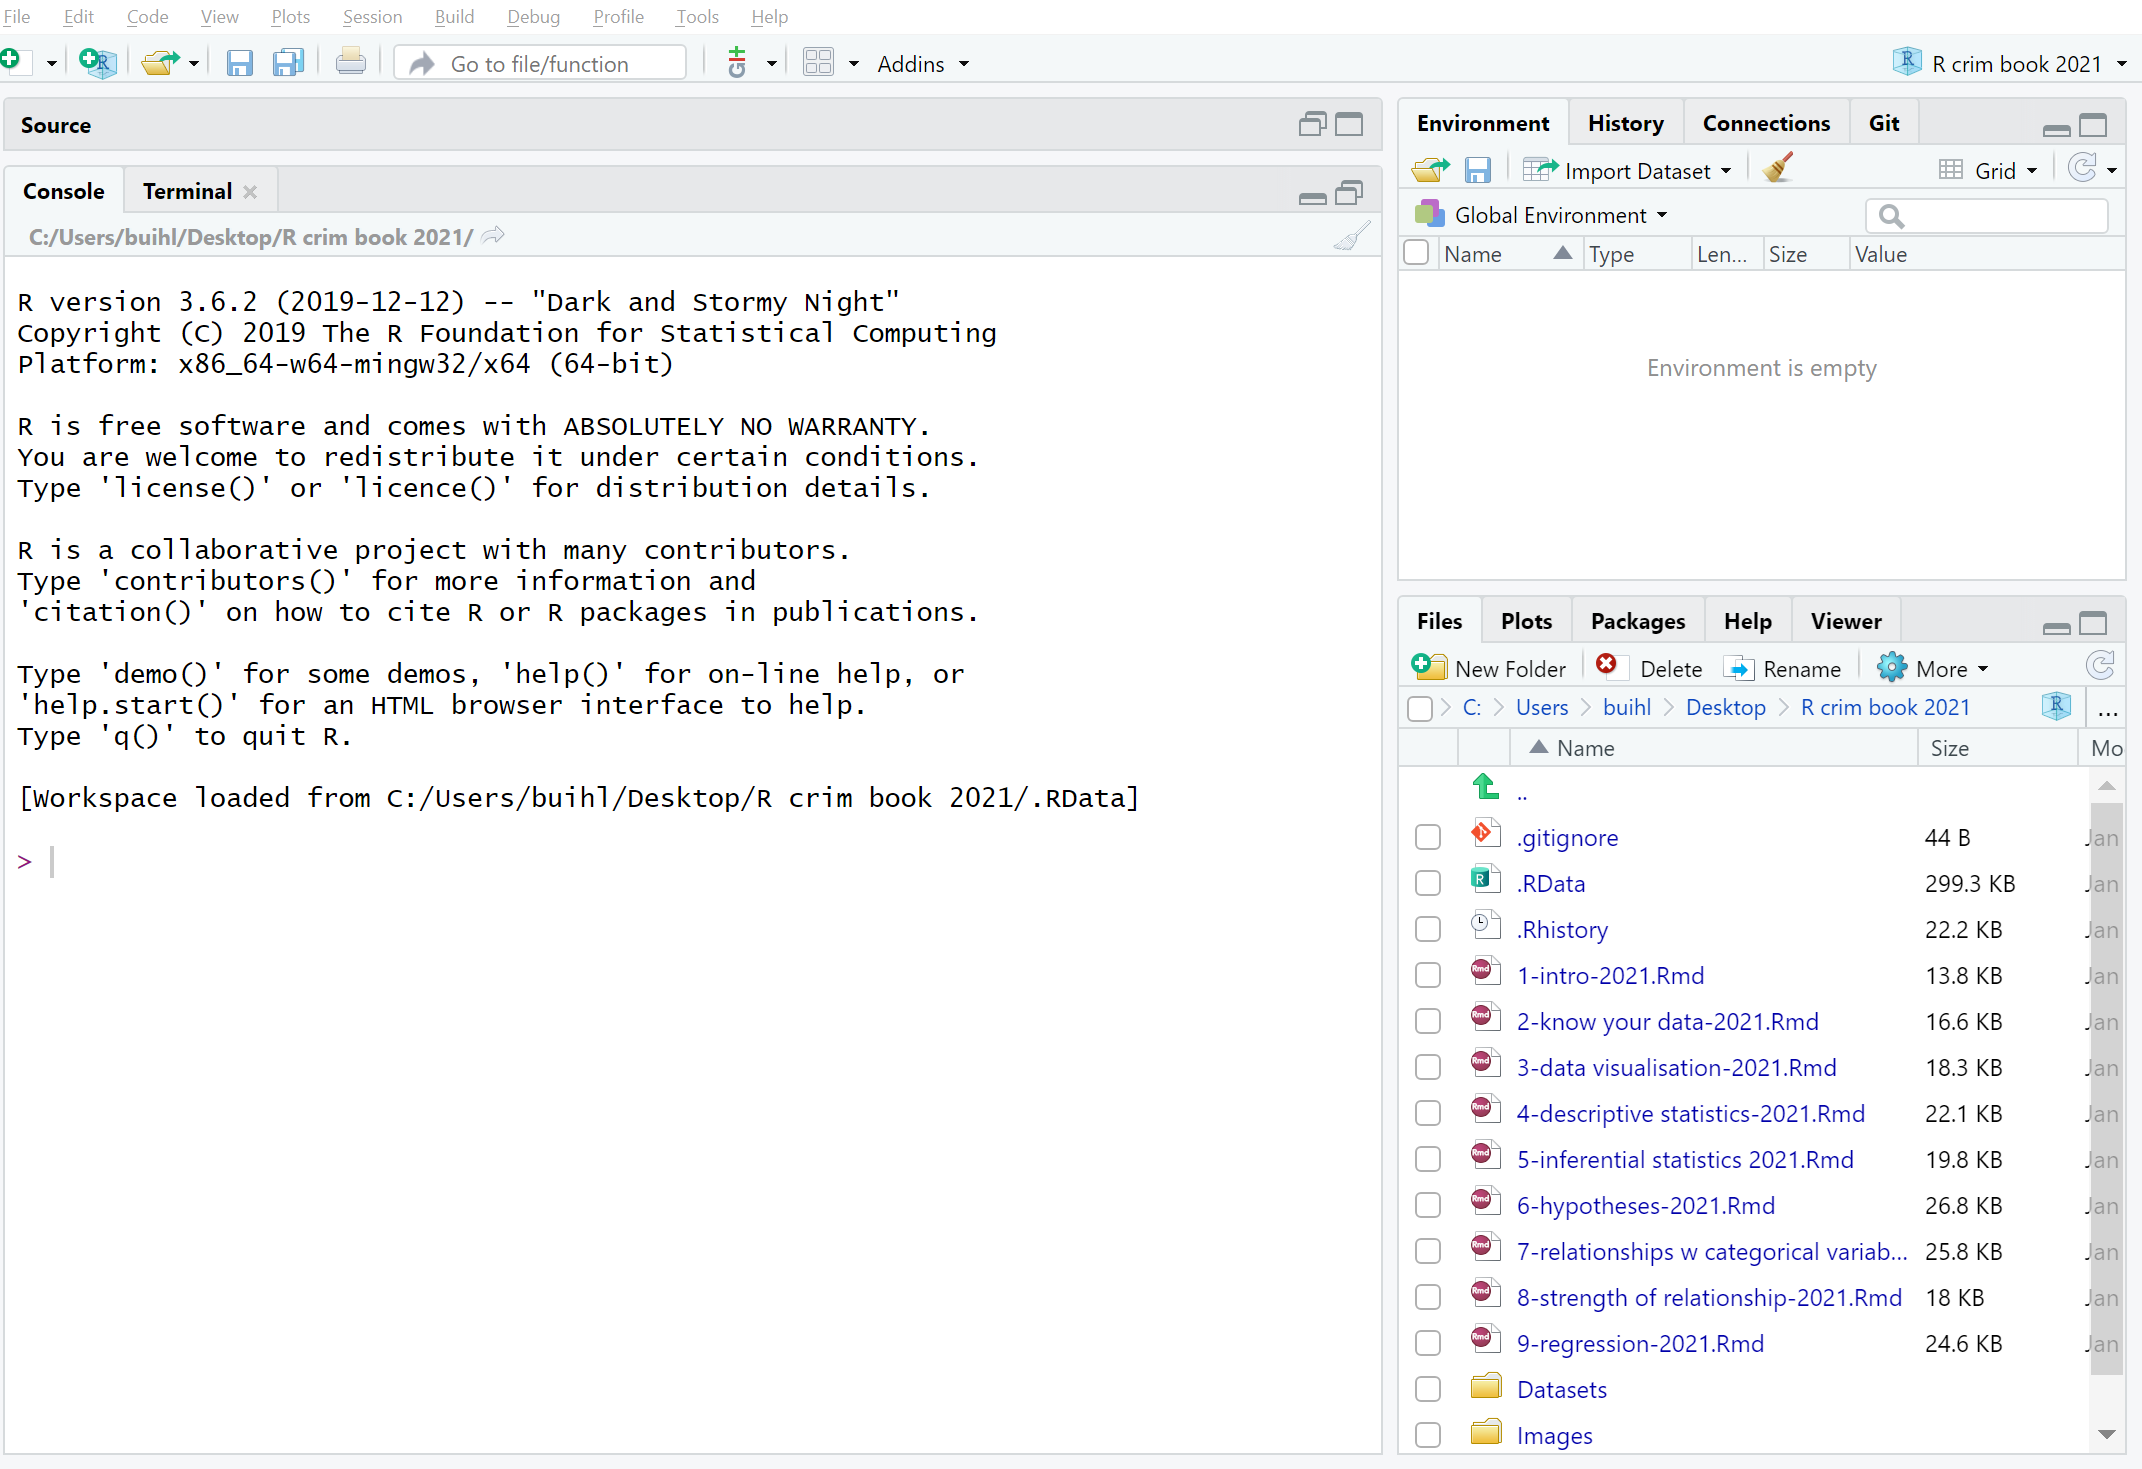
\includegraphics[width=0.8\textwidth,height=\textheight]{Images/rstudio1.png}
\caption{\textbf{Figure 1.1} R Studio interface}
\end{figure}

Figure 1.1 shows you what \texttt{RStudio} looks like when you first open it: three open panes.

The biggest one to your left is the main console, and it tells you what version of \texttt{R} you have.

When you start working in \texttt{Rstudio}, it is best to have \emph{four} open panes. \textbf{How?} Let us explore in the next activity.

\hypertarget{activity-3-opening-up-the-script-pane}{%
\subsubsection{Activity 3: Opening up the script pane}\label{activity-3-opening-up-the-script-pane}}

Figure 1.2: Click in the \emph{File} drop down Menu, select \emph{New File}, then \emph{R Script}.

\begin{figure}
\centering
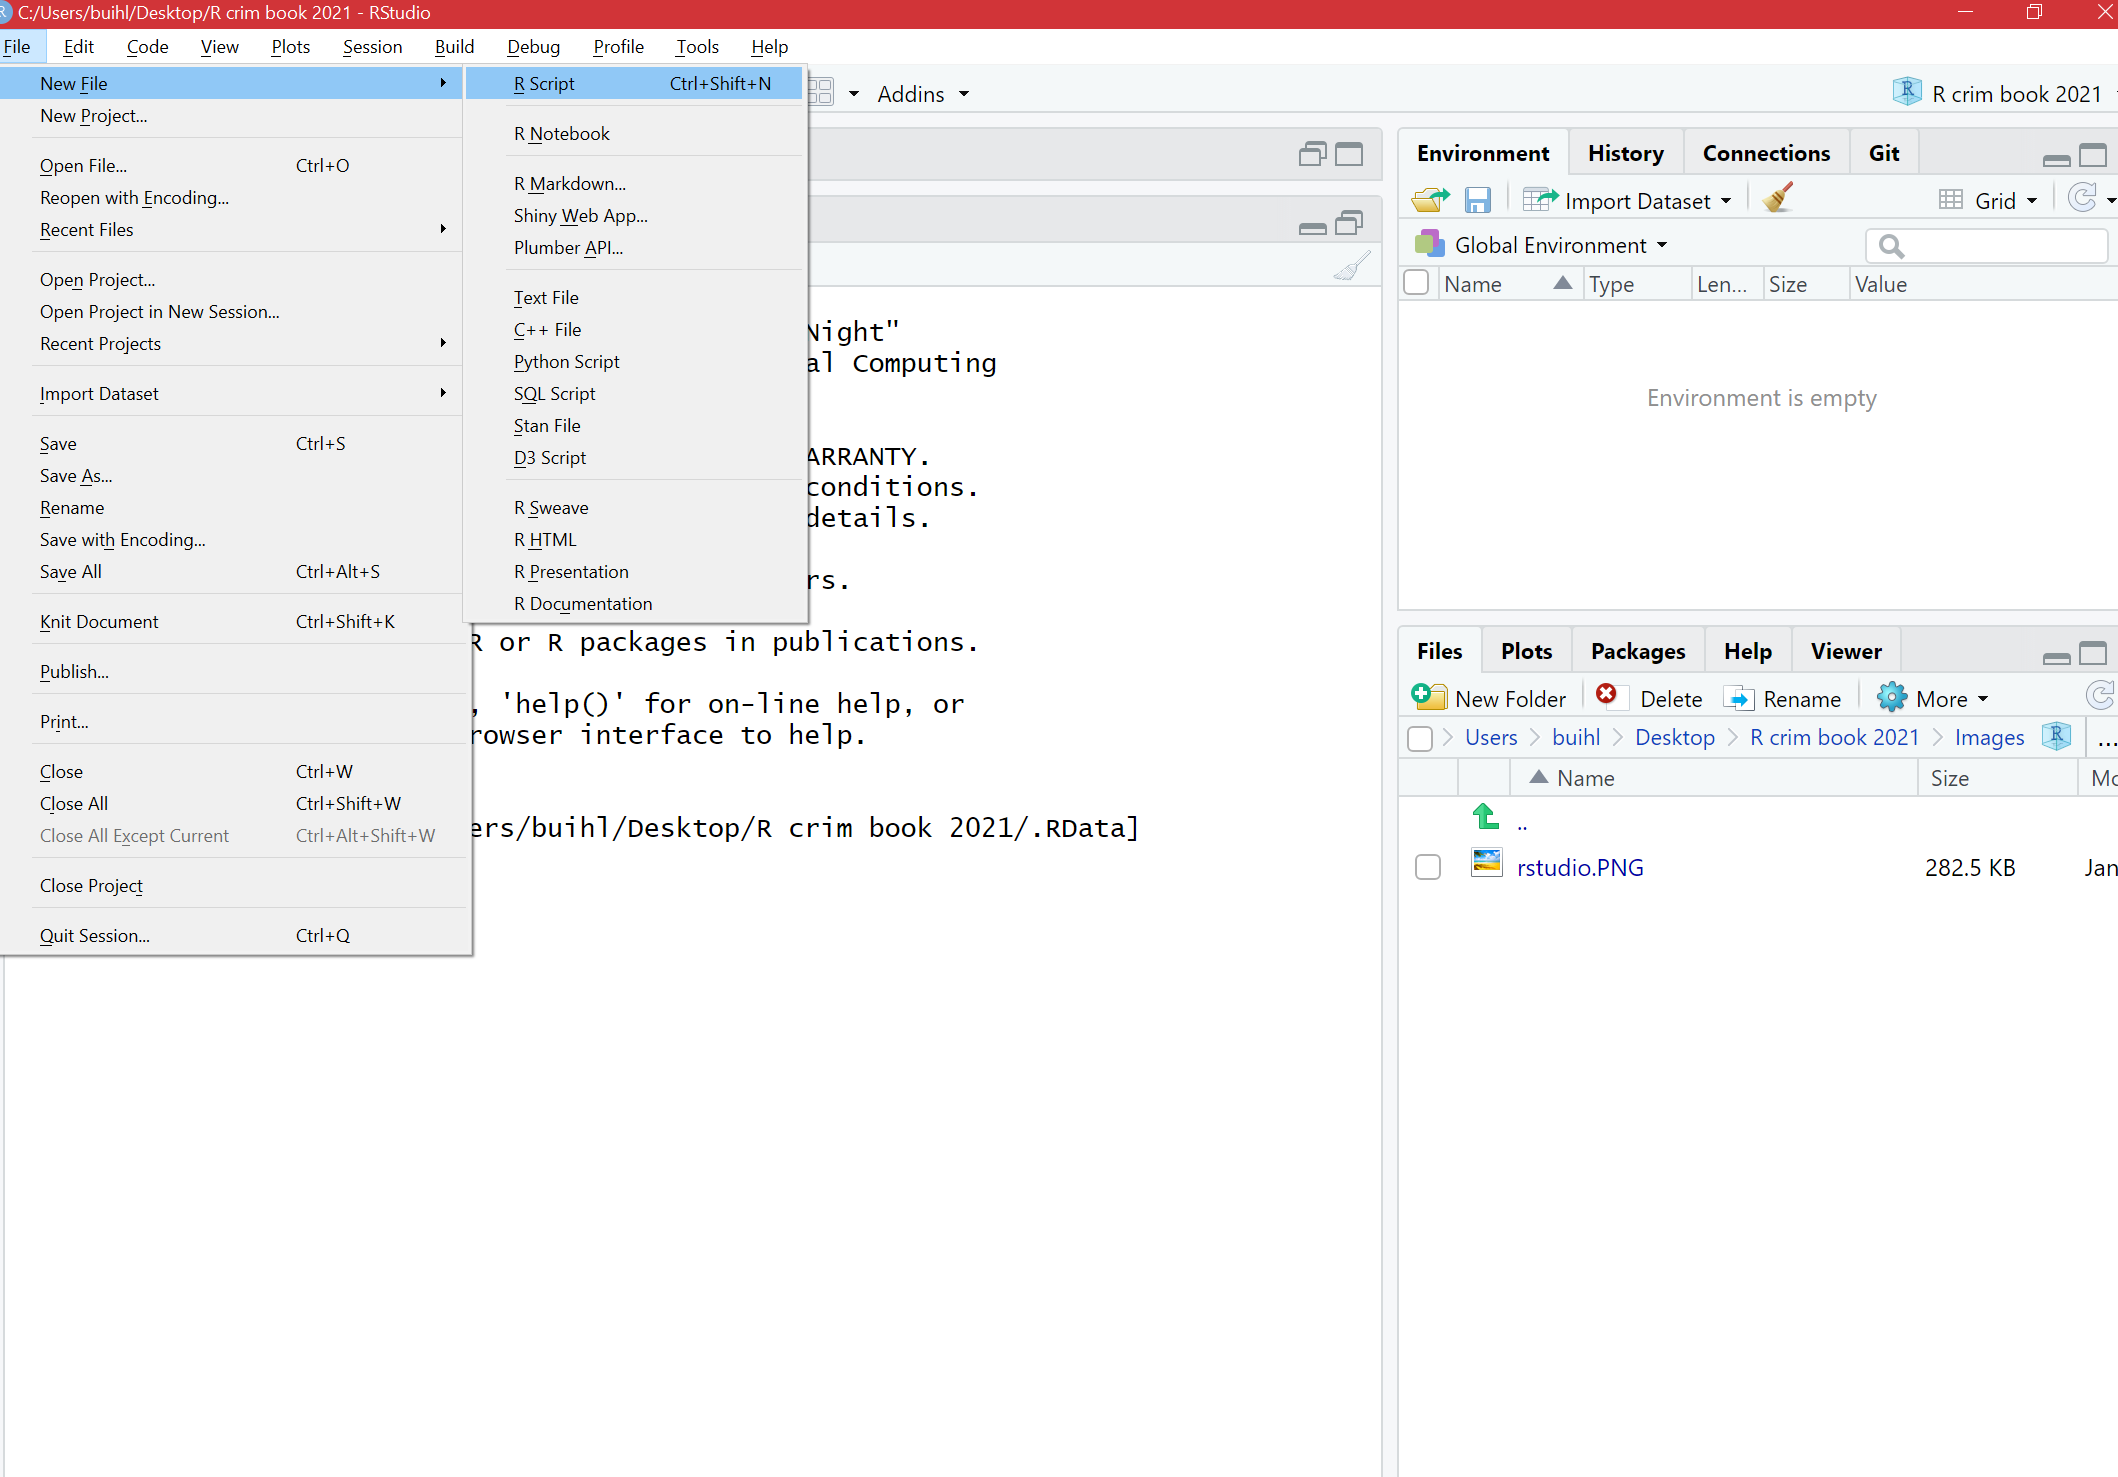
\includegraphics[width=0.7\textwidth,height=\textheight]{Images/R script.png}
\caption{\textbf{Figure 1.2} Creating an R Script}
\end{figure}

You can shift between different panes and re-size them with your mouse too.

\begin{figure}
\centering
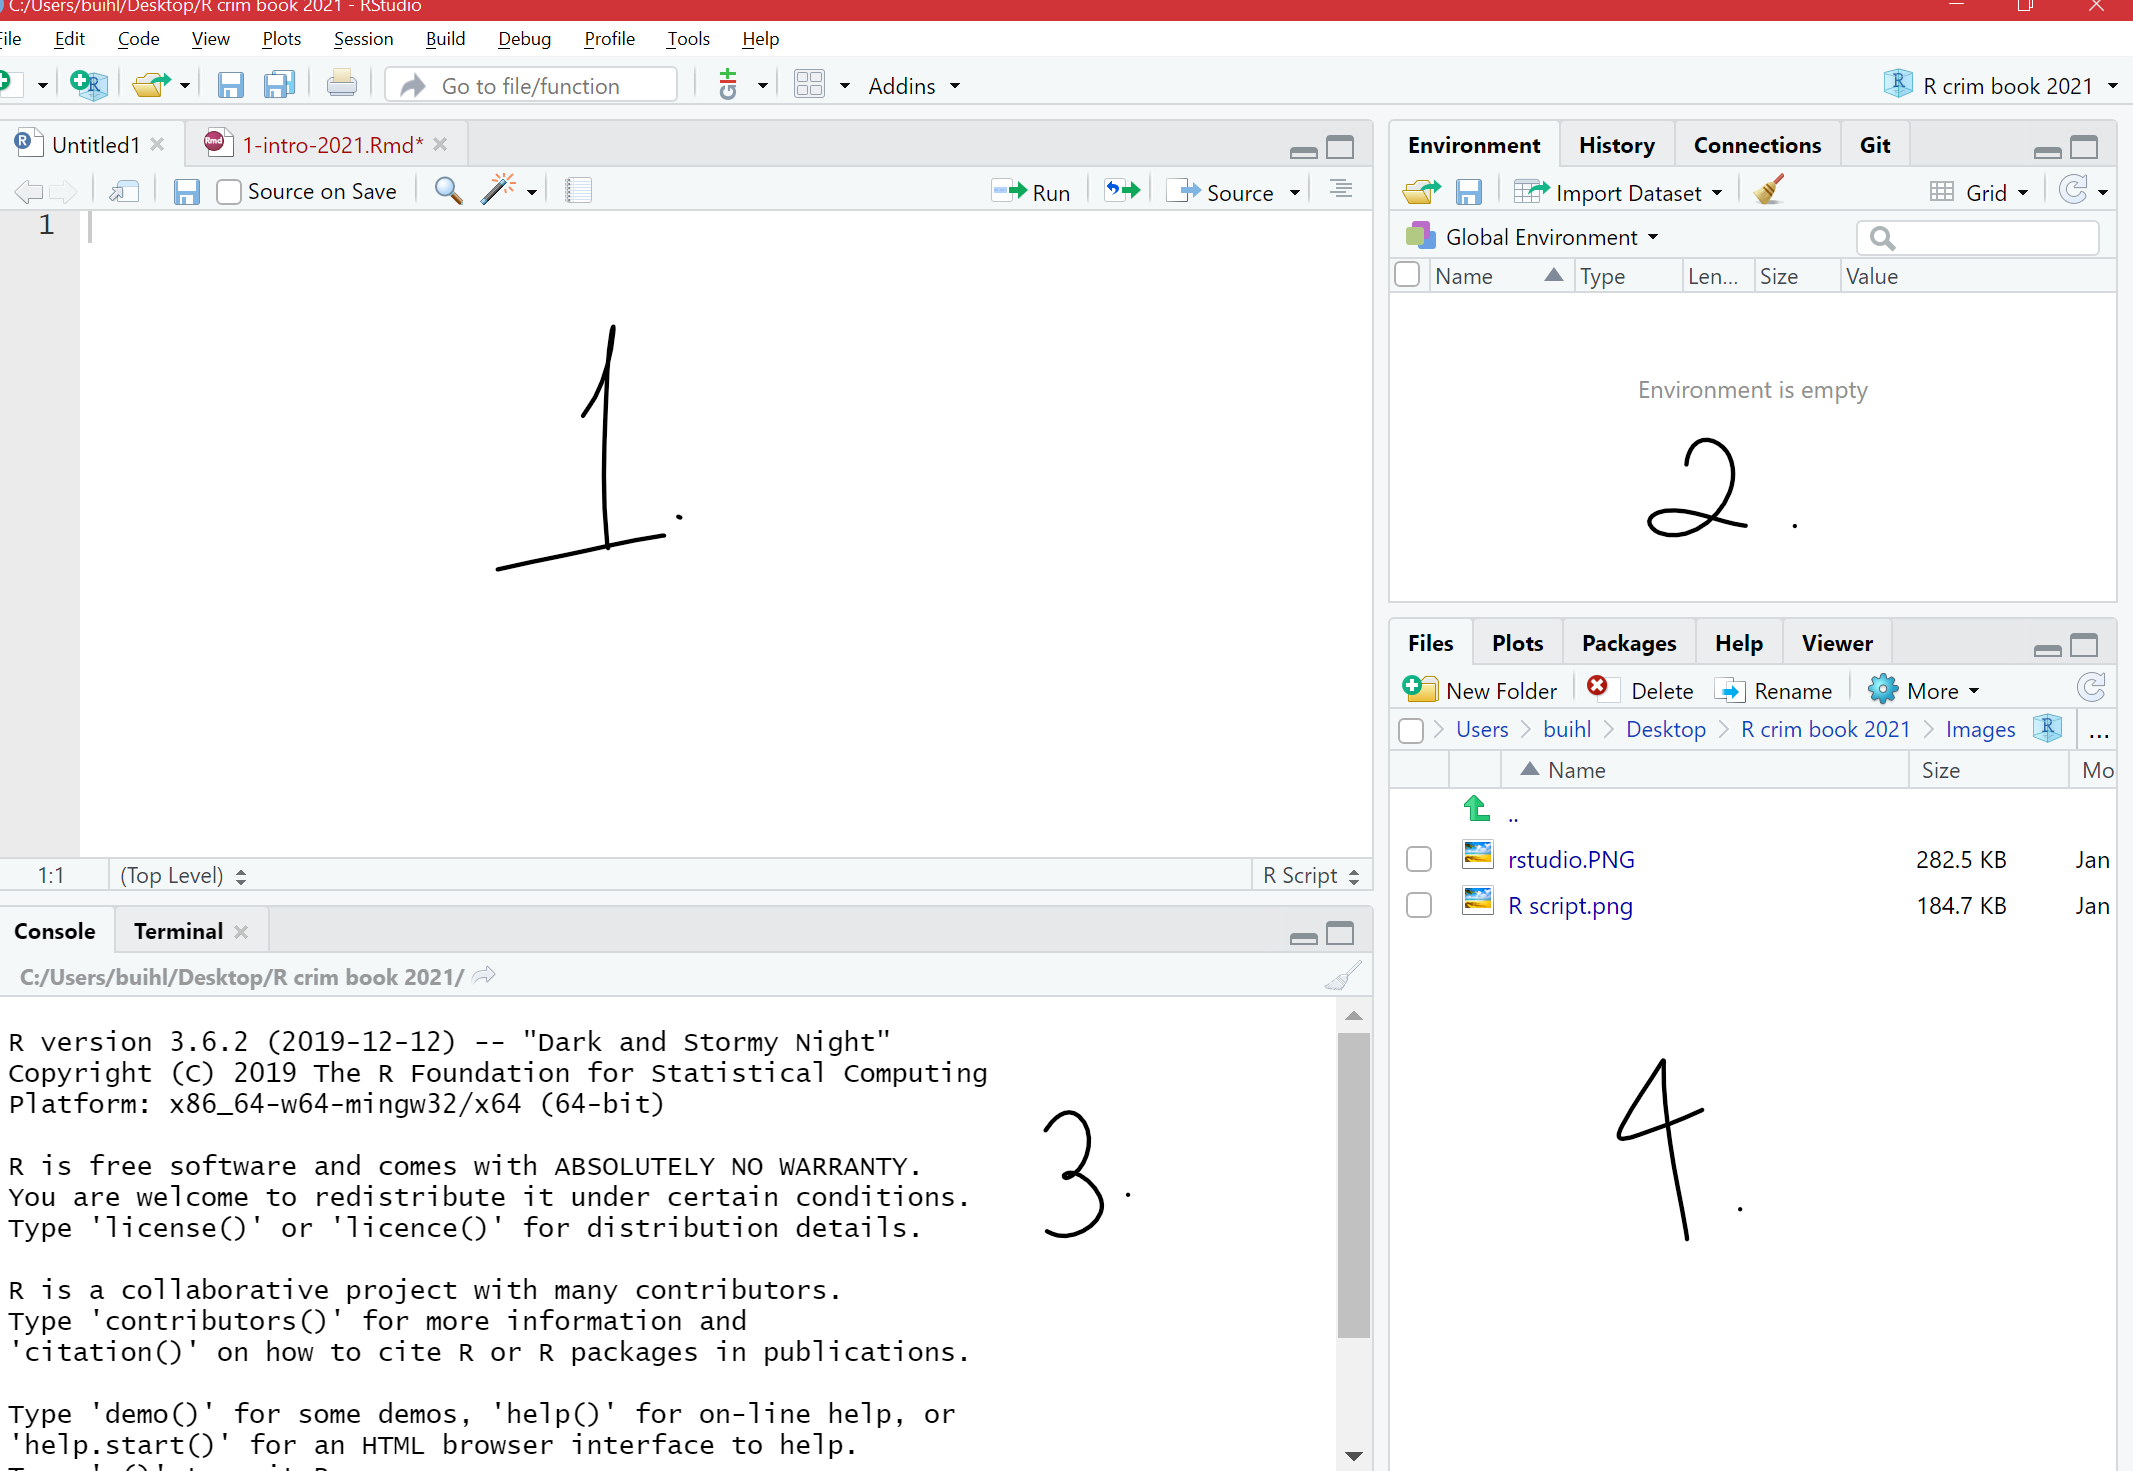
\includegraphics[width=0.7\textwidth,height=\textheight]{Images/main window.png}
\caption{\textbf{Figure 1.3} Main window in \texttt{RStudio}}
\end{figure}

\hypertarget{the-four-panes-of-r-studio}{%
\subsection{The four panes of R Studio}\label{the-four-panes-of-r-studio}}

The purposes of the four panes in Figure 1.3 are the following:

\begin{enumerate}
\def\labelenumi{\arabic{enumi}.}
\item
  \textbf{Script and data view}: where you type your programming code that tells \texttt{R} what you want to do. These are essentially instructions that you type and save as a \textbf{script}, so that you can return to it later to remember what you did and to share it with others so that they can reproduce what you did.
\item
  \textbf{Environment and history view}:
\end{enumerate}

\begin{enumerate}
\def\labelenumi{\roman{enumi})}
\item
  \emph{2.1 Environment} tab- gives you the names of all the (data) objects that you have defined during your current \texttt{R} session, including number of observations and rows in those objects. We learn more about objects later.
\item
  \emph{2.2 History} tab- shows you a history of all the code you have previously evaluated in the main console.
\end{enumerate}

\begin{enumerate}
\def\labelenumi{\arabic{enumi}.}
\setcounter{enumi}{2}
\tightlist
\item
  \textbf{Main console}: this is considered \texttt{R\textquotesingle{}s} heart, and it is where \texttt{R} evaluates the codes that you run. You can type your codes directly in the console, but for the sake of good habits, type them in the script and data view so you can save a record of them. Only type and run code from here if you want to debug or do some quick analysis.
\end{enumerate}

\begin{enumerate}
\def\labelenumi{\arabic{enumi}.}
\setcounter{enumi}{3}
\tightlist
\item
  \textbf{File directory, Plots, Packages, Help}:
\end{enumerate}

\begin{enumerate}
\def\labelenumi{\roman{enumi})}
\item
  \emph{4.1 Files} tab- allows you to see the files in the folder that is currently set as your working directory.
\item
  \emph{4.2 Plots} tab- you will see any data visualizations that you produce here. You have not produced any yet, so it is empty now.
\item
  \emph{4.3 Packages} tab- you will see the packages that are currently available to install. We will explain what these are soon, but know that they are an essential feature when working with \texttt{R}.
\item
  \emph{4.4 Help} tab- you can access further information on the various packages.
\end{enumerate}

\begin{center}\rule{0.5\linewidth}{0.5pt}\end{center}

\hypertarget{activity-4-interacting-with-the-4-panes}{%
\subsubsection{Activity 4: Interacting with the 4 panes}\label{activity-4-interacting-with-the-4-panes}}

In the previous activity, you opened up the `script' pane. We now write some code in it, and see what happens.

To do this, go to your open version of \texttt{R\ Studio}, and type in the script pane the following:

\begin{Shaded}
\begin{Highlighting}[]
\FunctionTok{print}\NormalTok{(}\StringTok{"Hello world!"}\NormalTok{)}
\end{Highlighting}
\end{Shaded}

When you have typed this, you will have typed your first bit of code. Yet nothing is happening? That is because you also have to \textbf{RUN} the code.

You can do this by highlighting the code you wish to run, and clicking on `run' in the top right hand corner:

\url{....}

When you `run' the code, it will print the text `Hello World!'(above in Figure 1.4) in the bottom pane, which is the \textbf{console}. That means you have written and executed your first line of code.

In the rest of the session, we will be unpacking how this all works, and getting more familiar and comfortable with using \texttt{R\ Studio}.

\begin{center}\rule{0.5\linewidth}{0.5pt}\end{center}

\hypertarget{customising-r-studio}{%
\subsection{Customising R Studio}\label{customising-r-studio}}

Did you know you can change the way \texttt{RStudio} looks? Click in the \emph{Tools} menu and select \emph{Global Options}. A pop-up window appears with various options:

\begin{figure}
\centering
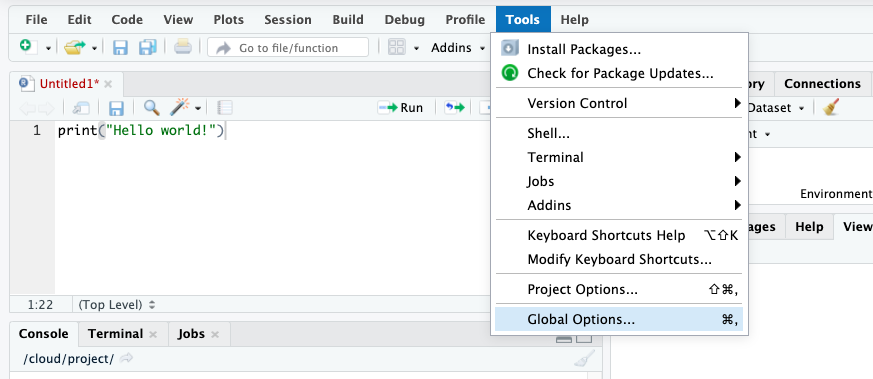
\includegraphics[width=0.7\textwidth,height=\textheight]{Images/tools_global_options.png}
\caption{\textbf{Figure 1.5} Selecting `Global Options'}
\end{figure}

Select \emph{Appearance}. Here, you can change things related to the appearance of \texttt{R\ Studio} like the font type and size, including the theme background that \texttt{R} will use as the interface.

\begin{figure}
\centering
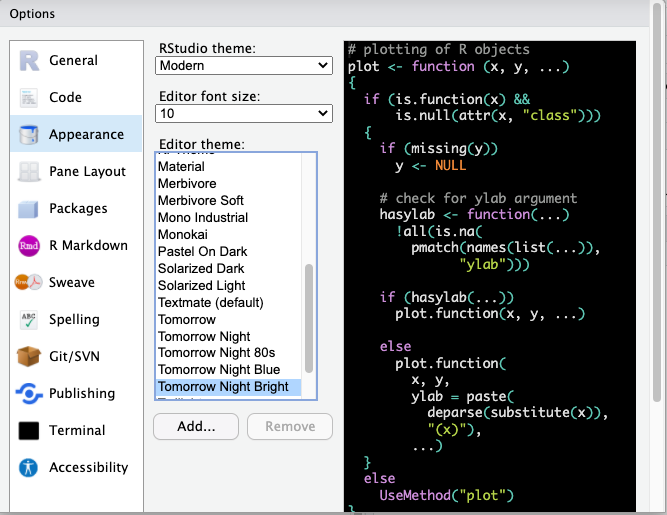
\includegraphics[width=0.7\textwidth,height=\textheight]{Images/appearance_choose_tomorrow_night_bright.png}
\caption{\textbf{Figure 1.6} Choosing a theme background}
\end{figure}

\emph{Tomorrow Night Bright} theme in Figure 1.7 is a recommendation because it is easier on your eyes with its dark background. You can preview and then click \emph{Apply} to select the one you like.

\begin{figure}
\centering
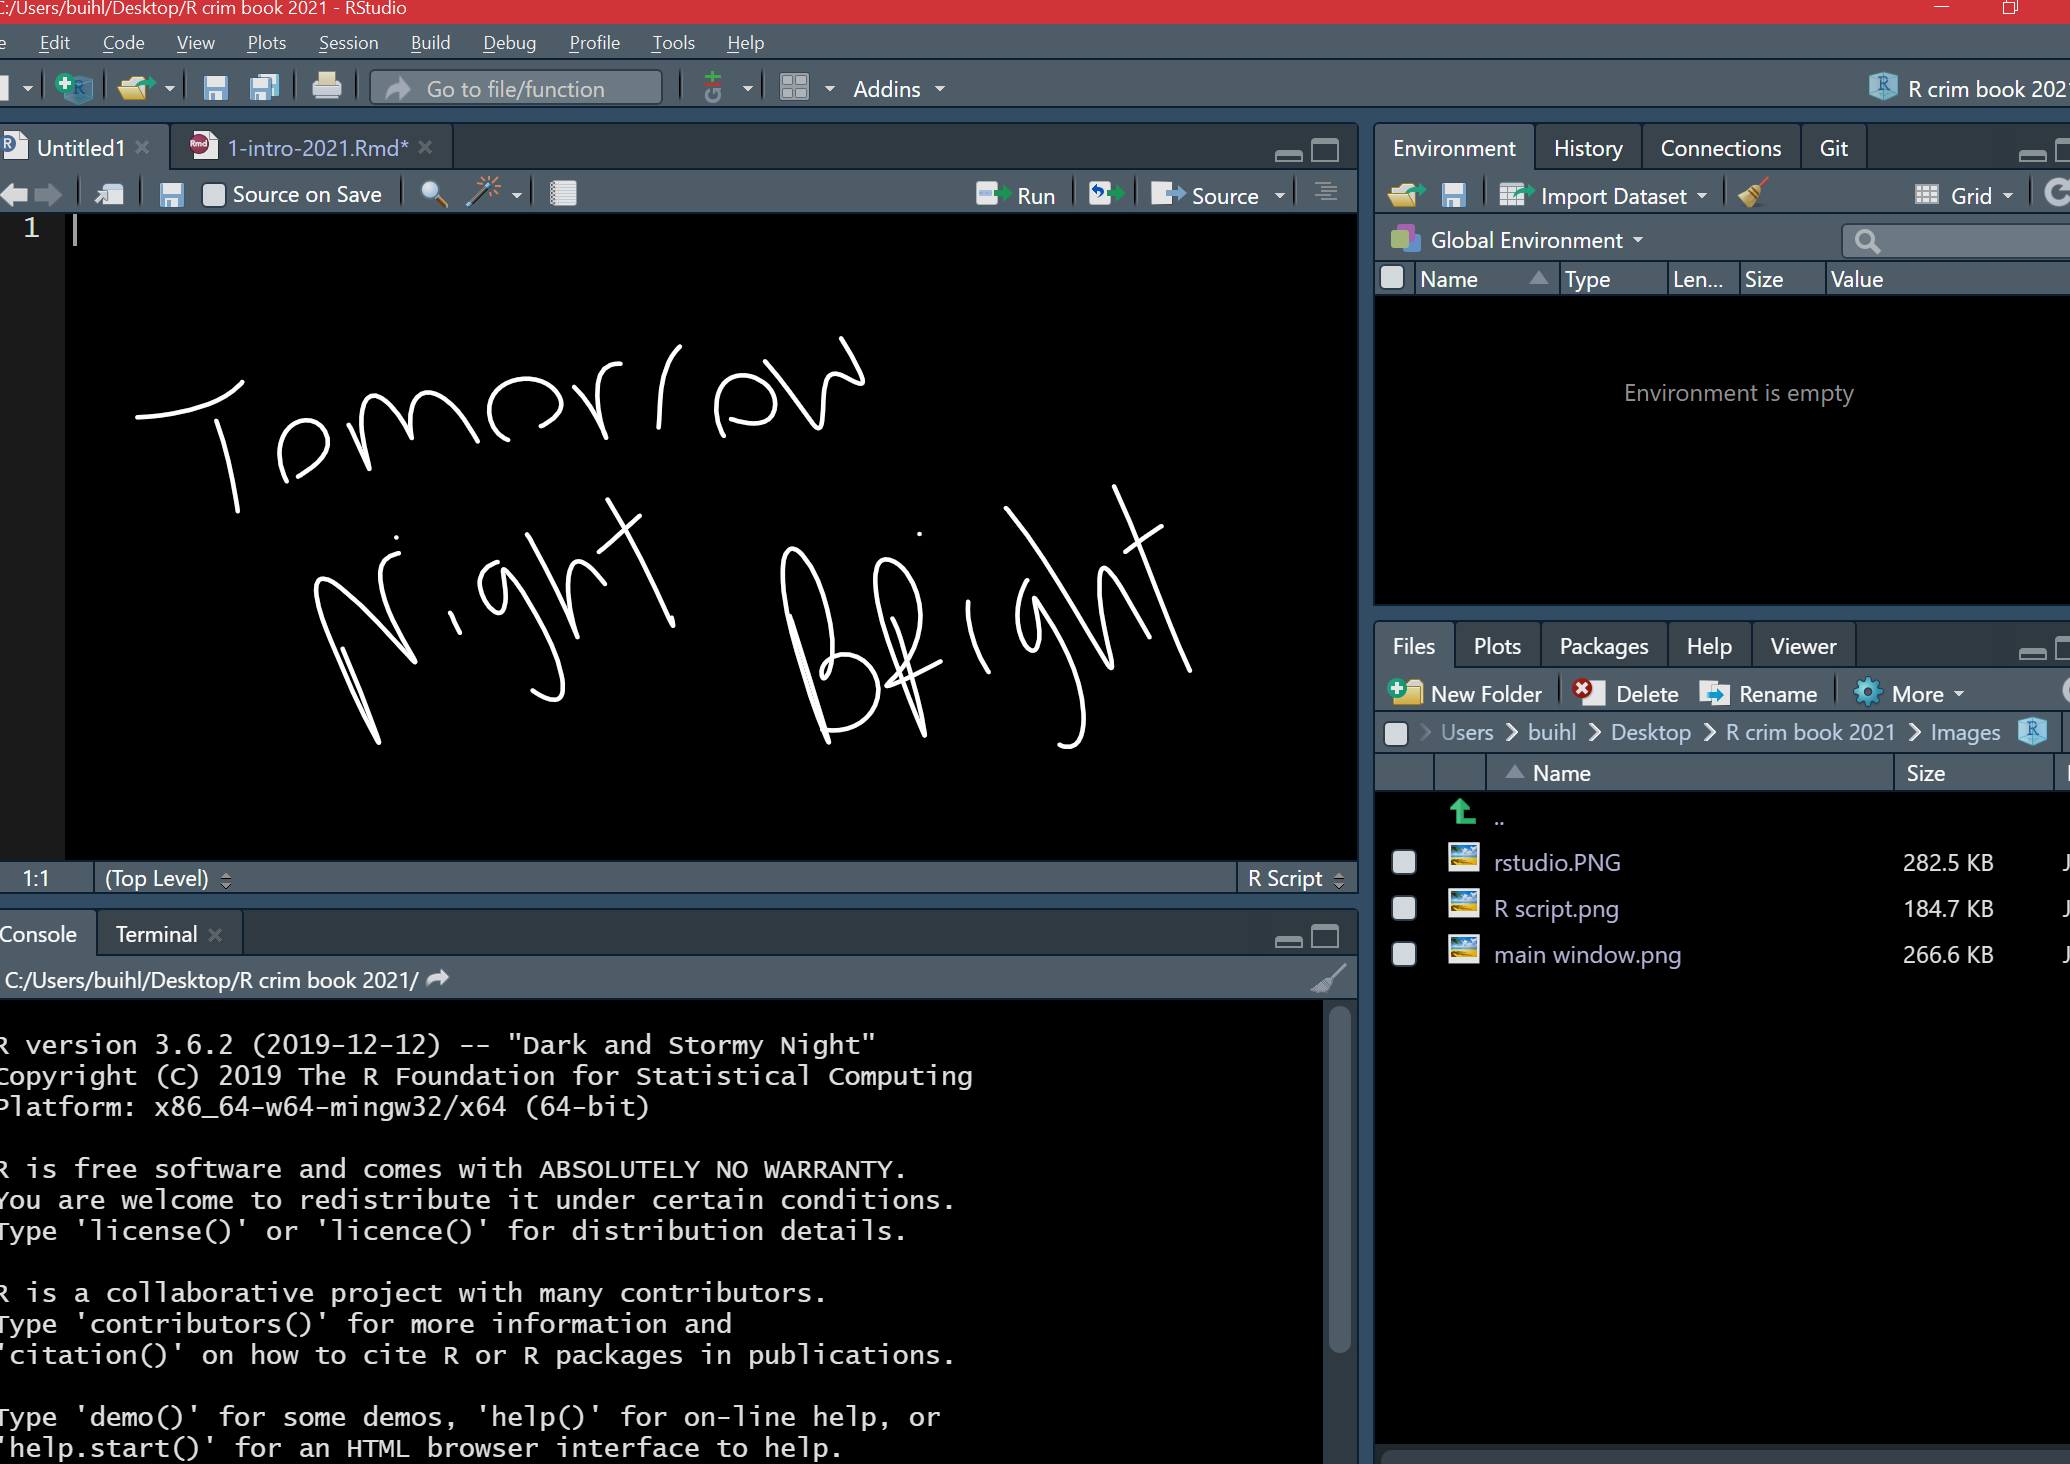
\includegraphics[width=0.55\textwidth,height=\textheight]{Images/tomorrow night bright.png}
\caption{\textbf{Figure 1.7} Tomorrow Night Bright Theme}
\end{figure}

\begin{center}\rule{0.5\linewidth}{0.5pt}\end{center}

\hypertarget{todays-3-topics}{%
\section{Today's 3 (TOPICS)}\label{todays-3-topics}}

Now that we have a basic understanding of \texttt{R}, we are ready to learn some building blocks. Each session of \emph{Modelling Criminological Data} will focus on three substantive topics, which are the key learning outcomes for each week. Today's topics are \textbf{operators and functions}, \textbf{objects}, and \textbf{packages}. Once you have mastered these three topics, you will be ready to start using \texttt{R} for data analysis!

\begin{center}\rule{0.5\linewidth}{0.5pt}\end{center}

\hypertarget{operators-and-functions}{%
\subsection{Operators and Functions}\label{operators-and-functions}}

\textbf{Operators} are symbols that tell \texttt{R} to do something specific like assigning values to vectors. They fall into four categories: arithmetic, relational, logical, and assignment. For now, let us type out and run some arithmetic operators:

\begin{Shaded}
\begin{Highlighting}[]
\CommentTok{\# Addition}
\DecValTok{5} \SpecialCharTok{+} \DecValTok{5}
\end{Highlighting}
\end{Shaded}

\begin{verbatim}
## [1] 10
\end{verbatim}

\begin{Shaded}
\begin{Highlighting}[]
\CommentTok{\# Subtraction}
\DecValTok{10} \SpecialCharTok{{-}} \DecValTok{3}
\end{Highlighting}
\end{Shaded}

\begin{verbatim}
## [1] 7
\end{verbatim}

\begin{Shaded}
\begin{Highlighting}[]
\CommentTok{\# Multiplication}
\DecValTok{2} \SpecialCharTok{*} \DecValTok{5}
\end{Highlighting}
\end{Shaded}

\begin{verbatim}
## [1] 10
\end{verbatim}

\begin{Shaded}
\begin{Highlighting}[]
\CommentTok{\# Division}
\DecValTok{6} \SpecialCharTok{/} \DecValTok{2}
\end{Highlighting}
\end{Shaded}

\begin{verbatim}
## [1] 3
\end{verbatim}

Did you \emph{Run} the arithmetic operators? The answers will have appeared, just like the above. If you are wondering what the \# symbol means in the coding above, these are called \textbf{comments}. They are annotations you can use in your \texttt{R\ script} to tell \texttt{R} that what comes right after the \textbf{\#} are not code to be ran. Comments are like your personal notes alongside your coding.

There are other operators we will come across like the \emph{and} operator (\texttt{\&}) and the \emph{or} operator (\texttt{\textbar{}}), which will be useful when we start to manipulate our data sets.

\hypertarget{activity-5-play-around-with-operators}{%
\subsubsection{Activity 5: Play around with operators}\label{activity-5-play-around-with-operators}}

Return to your open version of \texttt{R\ Studio}, and use this to find the answer to the following:

\begin{Shaded}
\begin{Highlighting}[]
\DecValTok{12329} \SpecialCharTok{+} \DecValTok{342980}
\DecValTok{18390} \SpecialCharTok{/} \DecValTok{348}
\end{Highlighting}
\end{Shaded}

The results should appear in the console pane and is known as your output.

\begin{center}\rule{0.5\linewidth}{0.5pt}\end{center}

\textbf{Functions} are similar to operators in that they \emph{do} things. The difference is that they are called by a certain name, usually a name which represents what they do, and they are followed by brackets \texttt{()}. Within the brackets, you can put whatever it is that you want the function to work with. For example, the code we wrote in Activity 4 was the \texttt{print()} function. This function told \texttt{R} to print into the console whatever we put in the brackets (``Hello world!'').

Same idea with a personalised greeting: if you want to print `Hello Reka', you will need to have ``Hello Reka'' inside the brackets:

\begin{Shaded}
\begin{Highlighting}[]
\FunctionTok{print}\NormalTok{(}\StringTok{"Hello Reka"}\NormalTok{)}
\end{Highlighting}
\end{Shaded}

\begin{verbatim}
## [1] "Hello Reka"
\end{verbatim}

Hello Reka.

There are so many functions in \texttt{R}. We will be learning many of them throughout our class. \texttt{Print} is fun, but most of the time, we will be using functions to help us with our data analysis. You might remember some Excel formulas we learned last semester from \emph{Making Sense of Criminological Data}. For example, getting the minimum, maximum, or mean of a list of numbers. \texttt{R} does this using functions in a very similar way.

For example, if we have a bunch of numbers, we just find the appropriate function to get the summary we want:

\begin{Shaded}
\begin{Highlighting}[]
\FunctionTok{mean}\NormalTok{(}\FunctionTok{c}\NormalTok{(}\DecValTok{10}\NormalTok{, }\DecValTok{34}\NormalTok{, }\DecValTok{5}\NormalTok{, }\DecValTok{3}\NormalTok{, }\DecValTok{77}\NormalTok{))}
\end{Highlighting}
\end{Shaded}

\begin{verbatim}
## [1] 25.8
\end{verbatim}

\begin{Shaded}
\begin{Highlighting}[]
\FunctionTok{min}\NormalTok{(}\FunctionTok{c}\NormalTok{(}\DecValTok{10}\NormalTok{, }\DecValTok{34}\NormalTok{, }\DecValTok{5}\NormalTok{, }\DecValTok{3}\NormalTok{, }\DecValTok{77}\NormalTok{))}
\end{Highlighting}
\end{Shaded}

\begin{verbatim}
## [1] 3
\end{verbatim}

\begin{Shaded}
\begin{Highlighting}[]
\FunctionTok{max}\NormalTok{(}\FunctionTok{c}\NormalTok{(}\DecValTok{10}\NormalTok{, }\DecValTok{34}\NormalTok{, }\DecValTok{5}\NormalTok{, }\DecValTok{3}\NormalTok{, }\DecValTok{77}\NormalTok{))}
\end{Highlighting}
\end{Shaded}

\begin{verbatim}
## [1] 77
\end{verbatim}

How exactly can you find the function you need? Throughout this class, you will learn a list that appears at the top of each lesson. A recommendation is to also create a `function cookbook', where you write down a list of functions, what the functions do, and some examples. Here is an example:

\begin{figure}
\centering
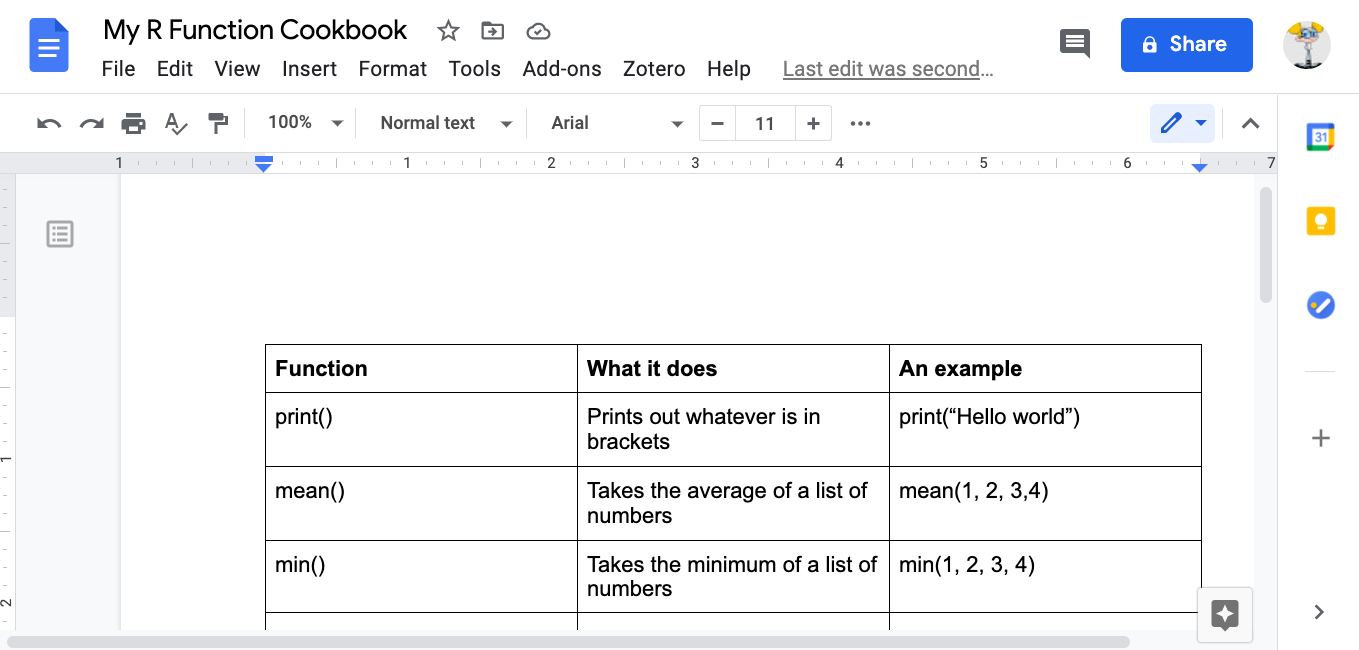
\includegraphics{Images/fn_cookbook.png}
\caption{\textbf{Figure 1.8} An example of a function cookbook}
\end{figure}

You can use google to make your cookbook, and the website \href{https://stackoverflow.com/}{stackoverflow}, in particular, can help you find the function you need. But be wary, especially in the beginning, that you understand what the function does. There can be several different functions for the same action. One good approach is to add a function of interest to your cookbook and ask the teaching team about what it does, and how it might be different to other functions that do the same thing.

\hypertarget{activity-6-play-around-with-functions}{%
\subsubsection{Activity 6: Play around with functions}\label{activity-6-play-around-with-functions}}

Have a guess of (or google) what you think is the function to get the median. Once you have your answer, write it in the shared google docs. Then, use it to get the median of the numbers 10, 34, 5, 3, 77.

Write the answer in your shared google doc (or note it down for yourself if in the quiet room).

The answer is further below, after the note:

\textbf{NOTE:} \texttt{R} is case-sensitive! For example:

\begin{Shaded}
\begin{Highlighting}[]
\CommentTok{\# Calculating the logarithm }
\FunctionTok{Log}\NormalTok{(}\DecValTok{100}\NormalTok{)}

\CommentTok{\# ERROR!}
\end{Highlighting}
\end{Shaded}

\begin{Shaded}
\begin{Highlighting}[]
\CommentTok{\# Instead, it should be:}
\FunctionTok{log}\NormalTok{(}\DecValTok{100}\NormalTok{)}
\end{Highlighting}
\end{Shaded}

\begin{verbatim}
## [1] 4.60517
\end{verbatim}

Okay, now you know these, the answer to Activity 6 was\ldots{}

\begin{Shaded}
\begin{Highlighting}[]
\FunctionTok{median}\NormalTok{(}\FunctionTok{c}\NormalTok{(}\DecValTok{10}\NormalTok{, }\DecValTok{34}\NormalTok{, }\DecValTok{5}\NormalTok{, }\DecValTok{3}\NormalTok{, }\DecValTok{77}\NormalTok{))}
\end{Highlighting}
\end{Shaded}

\begin{verbatim}
## [1] 10
\end{verbatim}

Now let us move on to our second key topic for today: objects!

\begin{center}\rule{0.5\linewidth}{0.5pt}\end{center}

\hypertarget{objects}{%
\subsection{Objects}\label{objects}}

Everything that exists in \texttt{R} is an \textbf{object}. Think of objects as boxes where you put things in. Imagine a big, empty cardboard box. We can create this big empty box in \texttt{R} by simply giving it a name. Usually, you want your object (`box') to have a good descriptive name, which will tell others what is in it. Imagine moving house. If you have a cardboard box full of plates, you might want to label it `plates'. That way, when carrying, you know to be careful, and when unpacking, you know its contents will go in the kitchen. On the other hand, if you named it `box1', then this is a lot less helpful when it comes to unpacking.

\hypertarget{activity-7-creating-an-object}{%
\subsubsection{Activity 7: Creating an object}\label{activity-7-creating-an-object}}

Let us create an object called `plates'. To do this, you go to your script, and type `plates'.

\begin{figure}
\centering
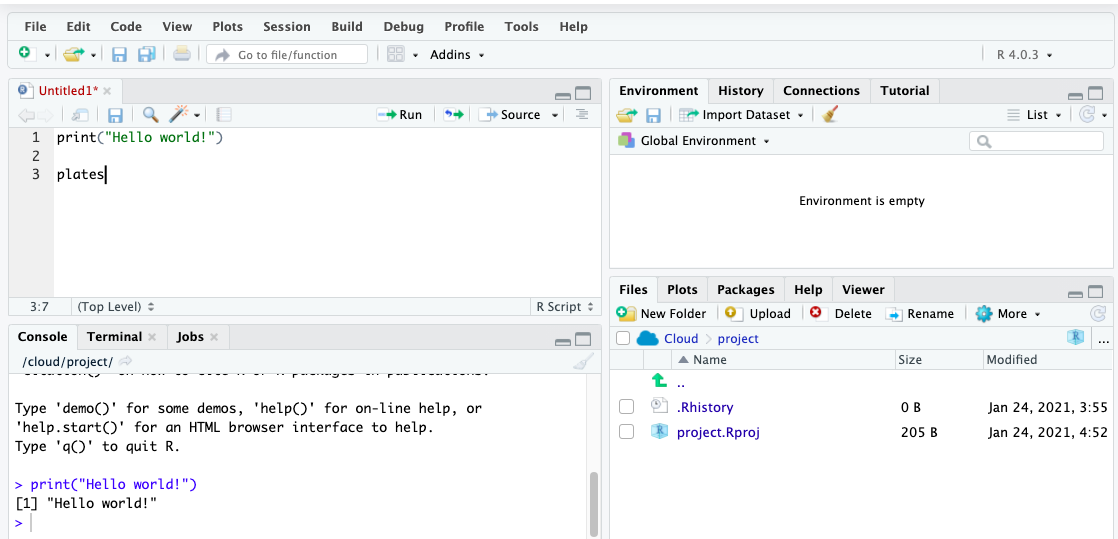
\includegraphics{Images/plates.png}
\caption{\textbf{Figure 1.9} Typing `Plates' in the script}
\end{figure}

But if you run this code, you will get an error. Let's see:

\url{....}

You will see the phrase `Error: object plates not found'. This is because you have not yet put anything inside the plates `box'. Remember objects are like boxes,so there must be something inside our object `plates'. In order for this object to exist, you have to put something inside it, or in \texttt{R}-speak \emph{assign it some value}.

Therefore, we make an object by using an \emph{assignment operator} ( \texttt{\textless{}-} ). In other words, we assign something to an object (i.e., put something in the box). For example:

\begin{Shaded}
\begin{Highlighting}[]
\NormalTok{plates }\OtherTok{\textless{}{-}} \StringTok{"yellow plate"}
\end{Highlighting}
\end{Shaded}

Now if we run this, we will see no error message, but instead, we will see the \texttt{plates} object appear in our \emph{environment pane}:

\url{....}

Here are some more examples to illustrate:

\begin{Shaded}
\begin{Highlighting}[]
\CommentTok{\# Putting \textquotesingle{}10\textquotesingle{} in the \textquotesingle{}a\textquotesingle{} box}
\NormalTok{a }\OtherTok{\textless{}{-}} \DecValTok{10}

\CommentTok{\# Putting \textquotesingle{}Hello!\textquotesingle{} in the \textquotesingle{}abc123\textquotesingle{} box}
\NormalTok{abc123 }\OtherTok{\textless{}{-}} \StringTok{"Hello!"}
\end{Highlighting}
\end{Shaded}

In these examples, we are putting the value of \texttt{10} into the object \texttt{a}, and the value of `Hello!' into the object \texttt{abc123}.

Earlier, we introduced you to the Environment and History pane. We mentioned that it lists objects you defined. After making the `a' and `abc123' objects, they should appear in that very pane under the \texttt{Environment} tab.

\begin{center}\rule{0.5\linewidth}{0.5pt}\end{center}

\hypertarget{types-of-objects}{%
\subsubsection{Types of objects}\label{types-of-objects}}

Why are objects important? They are so because we will be storing everything in our data analysis process in these objects. Depending on what is inside them, they can become a different type of object. Here are some examples:

\textbf{Data structures} are important objects that store your data, and there are five main types but we focus on three for this course:

\begin{enumerate}
\def\labelenumi{\arabic{enumi}.}
\tightlist
\item
  \emph{(atomic) vector}: an ordered set of elements that are of the same \emph{class}. Vectors are a basic data structure in \texttt{R}. Below are five different classes of vectors:
\end{enumerate}

\begin{Shaded}
\begin{Highlighting}[]
\CommentTok{\# 1. numeric vector with three elements}
\NormalTok{my\_1st\_vector }\OtherTok{\textless{}{-}} \FunctionTok{c}\NormalTok{(}\FloatTok{0.5}\NormalTok{, }\FloatTok{8.9}\NormalTok{, }\FloatTok{0.6}\NormalTok{) }

\CommentTok{\# 2. integer vector with addition of L at the end of the value}
\NormalTok{my\_2nd\_vector }\OtherTok{\textless{}{-}} \FunctionTok{c}\NormalTok{(1L, 2L, 3L)  }

\CommentTok{\# 3. logical vector}
\NormalTok{my\_3rd\_vector }\OtherTok{\textless{}{-}} \FunctionTok{c}\NormalTok{(}\ConstantTok{TRUE}\NormalTok{, }\ConstantTok{FALSE}\NormalTok{, }\ConstantTok{FALSE}\NormalTok{) }
\CommentTok{\# \textquotesingle{}my\_4th\_vector\textquotesingle{} creates a logical vector using abbreviations of True and False, but you should use the full words instead}
\NormalTok{my\_4th\_vector }\OtherTok{\textless{}{-}} \FunctionTok{c}\NormalTok{(T, F) }

\CommentTok{\# 4. character vector}
\NormalTok{my\_5th\_vector }\OtherTok{\textless{}{-}} \FunctionTok{c}\NormalTok{(}\StringTok{"a"}\NormalTok{, }\StringTok{"b"}\NormalTok{, }\StringTok{"c"}\NormalTok{) }

\CommentTok{\# 5. complex vector (we will not use this for our class)}
\NormalTok{my\_6th\_vector }\OtherTok{\textless{}{-}} \FunctionTok{c}\NormalTok{(}\DecValTok{1}\SpecialCharTok{+}\NormalTok{0i, }\DecValTok{2}\SpecialCharTok{+}\NormalTok{4i) }
\end{Highlighting}
\end{Shaded}

\begin{enumerate}
\def\labelenumi{\arabic{enumi}.}
\setcounter{enumi}{1}
\tightlist
\item
  \emph{lists}: technically they, too, are vectors but they are more complex because they are not restricted on the length, structure, or class of the included elements. For example, to create a list containing strings, numbers, vectors and a logical, use the \texttt{list()} function, and inside the brackets, put everything that you want to combine into a list:
\end{enumerate}

\begin{Shaded}
\begin{Highlighting}[]
\NormalTok{list\_data }\OtherTok{\textless{}{-}} \FunctionTok{list}\NormalTok{(}\StringTok{"teal"}\NormalTok{, }\StringTok{"sky blue"}\NormalTok{, }\FunctionTok{c}\NormalTok{(}\DecValTok{10}\NormalTok{, }\DecValTok{5}\NormalTok{, }\DecValTok{10}\NormalTok{), }\ConstantTok{TRUE}\NormalTok{, }\FloatTok{68.26}\NormalTok{, }\FloatTok{95.46}\NormalTok{, }\FloatTok{99.7}\NormalTok{) }
\end{Highlighting}
\end{Shaded}

Above, we created \texttt{list\_data}, an object that contains all those things that we put inside the \texttt{list()} function. This function serves to create a list from combining everything that is put inside its brackets.

We then use the \texttt{class()} function to confirm that the objects have been defined as a list:

\begin{Shaded}
\begin{Highlighting}[]
\FunctionTok{class}\NormalTok{(list\_data)}
\end{Highlighting}
\end{Shaded}

\begin{verbatim}
## [1] "list"
\end{verbatim}

\begin{enumerate}
\def\labelenumi{\arabic{enumi}.}
\setcounter{enumi}{2}
\tightlist
\item
  \emph{data frames}: also stores elements but differ from lists because they are defined by their number of columns and rows; the vectors (columns) must be of the same length. Data frames can contain different classes but each column must be of the same class. (More on class next week.) For example, if you want to combine some related vectors to make a data frame on violent American cities, use the function \texttt{data.frame()}:
\end{enumerate}

\begin{Shaded}
\begin{Highlighting}[]
\CommentTok{\# Making some relevant vectors}
\NormalTok{TopVioCities }\OtherTok{\textless{}{-}} \FunctionTok{c}\NormalTok{(}\StringTok{"St. Louis"}\NormalTok{, }\StringTok{"Detroit"}\NormalTok{, }\StringTok{"Baltimore"}\NormalTok{) }\CommentTok{\# some violent US cities}
\NormalTok{VioRatePer1k }\OtherTok{=} \FunctionTok{c}\NormalTok{(}\FloatTok{20.8}\NormalTok{, }\FloatTok{20.6}\NormalTok{, }\FloatTok{20.3}\NormalTok{) }\CommentTok{\# their violence rates per 1,000 persons}
\NormalTok{State }\OtherTok{\textless{}{-}} \FunctionTok{c}\NormalTok{(}\StringTok{"Missouri"}\NormalTok{, }\StringTok{"Michigan"}\NormalTok{, }\StringTok{"Maryland"}\NormalTok{) }\CommentTok{\# in what states are these cities found}

\CommentTok{\#Join the newly created vectors to make a data frame called \textquotesingle{}df\textquotesingle{}}
\NormalTok{df}\OtherTok{\textless{}{-}}\FunctionTok{data.frame}\NormalTok{(TopVioCities, VioRatePer1k, State)}
\end{Highlighting}
\end{Shaded}

We can then view the data frame, `df', with the \texttt{View()} function in which a tab will appear containing our vectors:

\begin{Shaded}
\begin{Highlighting}[]
\FunctionTok{View}\NormalTok{(df)}
\end{Highlighting}
\end{Shaded}

\begin{center}\rule{0.5\linewidth}{0.5pt}\end{center}

\hypertarget{activity-8-doing-things-to-objects}{%
\subsubsection{Activity 8: Doing things to objects}\label{activity-8-doing-things-to-objects}}

We have learned what functions are (i.e., things that do things) and what operators are (i.e., symbols that do things) as well as what are objects (i.e., the boxes that hold things). We also saw some functions which helped us create objects. Functions can also do things to objects. For example, we saw the function \texttt{class()} that told us what kind of object \texttt{list\_data} was, and \texttt{View()} which allowed us to have a look at our dataframe we called \texttt{df}.

Let us look back at our \texttt{plates} object. Remember it was the object that held our kitchen items, specifically that beloved yellow plate. We added `yellow plate' to it. Now let us add some more plates (we like to collect plates apparently) and let us use the concatenate \texttt{c()} function for this again:

\begin{Shaded}
\begin{Highlighting}[]
\NormalTok{plates }\OtherTok{\textless{}{-}} \FunctionTok{c}\NormalTok{(}\StringTok{"yellow plate"}\NormalTok{, }\StringTok{"purple plate"}\NormalTok{, }\StringTok{"silver plate"}\NormalTok{, }\StringTok{"orange bowl"}\NormalTok{)}
\end{Highlighting}
\end{Shaded}

Let us say that we suddenly forgot what was in our object called `plates'. Like what we learned earlier, we use the function \texttt{print()} to see what is inside this object:

\begin{Shaded}
\begin{Highlighting}[]
\FunctionTok{print}\NormalTok{(plates)}
\end{Highlighting}
\end{Shaded}

\begin{verbatim}
## [1] "yellow plate" "purple plate" "silver plate" "orange bowl"
\end{verbatim}

This can apply to obtaining the mean, the minimum, and maximum. You could assign those statistics to an object this time:

\begin{Shaded}
\begin{Highlighting}[]
\NormalTok{nums }\OtherTok{\textless{}{-}} \FunctionTok{c}\NormalTok{(}\DecValTok{10}\NormalTok{, }\DecValTok{34}\NormalTok{, }\DecValTok{5}\NormalTok{, }\DecValTok{3}\NormalTok{, }\DecValTok{77}\NormalTok{)}
\end{Highlighting}
\end{Shaded}

Now if we want to know the mean, we can take the mean of the object \texttt{nums}, which we just created:

\begin{Shaded}
\begin{Highlighting}[]
\FunctionTok{mean}\NormalTok{(nums)}
\end{Highlighting}
\end{Shaded}

\begin{verbatim}
## [1] 25.8
\end{verbatim}

The object we will use most frequently though is data frames. Much like how we worked with spreadsheets in Excel in \emph{Making Sense of Criminological Data}, we will be working with dataframes in \texttt{R}.

We had created a dataframe called \texttt{df} previously. If you have not yet created this dataframe in your own \texttt{R\ Studio}, do this now. You should have the object \texttt{df} in your environment. When you run \texttt{View(df)}, you should see this dataset:

\begin{figure}
\centering
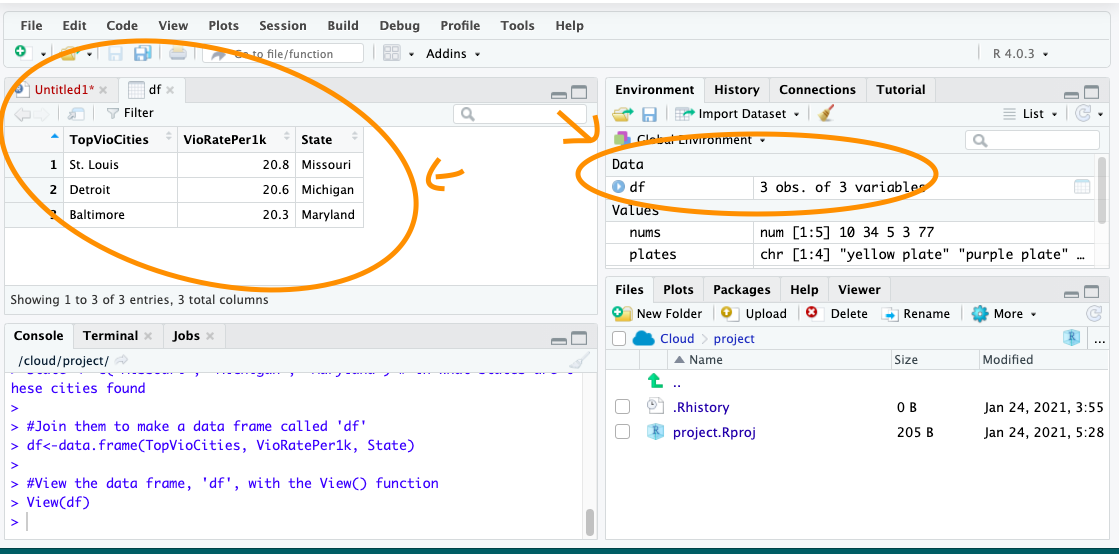
\includegraphics{Images/df_view.png}
\caption{\textbf{Figure 1.12} The data frame `df'}
\end{figure}

To do something to an entire dataframe, we would use the name of the object (\texttt{df}) to refer to it. In the case of the \texttt{View()} function, we want to see all that is contained in \texttt{df}, so we will type \texttt{View(df)}. On the other hand, if we want to refer to only one \emph{variable} or column in the data, (recall last semester - each variable is held in each column) there is a special notation to do this -- \$

To refer to a variable inside a dataframe, you use:

\(dataframe name + \$ + variable name\)

For example, to refer to the variable \texttt{VioRatePer1k}, we use the notation \texttt{df\$VioRatePer1k}.

And if we wanted to view only that variable, we use:

\begin{Shaded}
\begin{Highlighting}[]
\FunctionTok{View}\NormalTok{(df}\SpecialCharTok{$}\NormalTok{VioRatePer1k)}
\end{Highlighting}
\end{Shaded}

You should see:

\begin{figure}
\centering
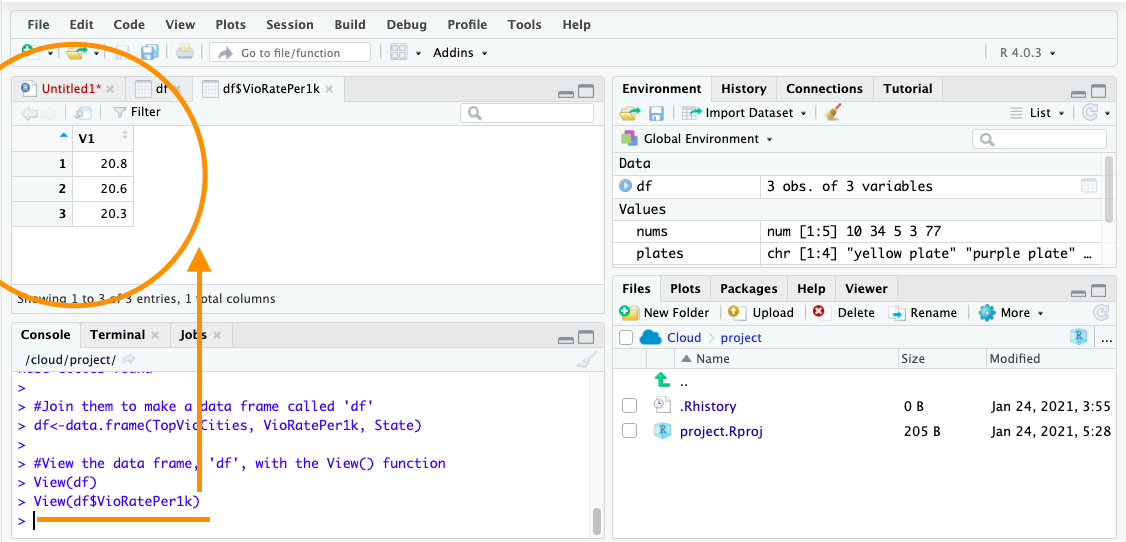
\includegraphics{Images/view_col_only.png}
\caption{\textbf{Figure 1.13} Viewing df\$VioRatePer1k}
\end{figure}

Say we wanted to know the mean violence rate across our units of analysis, the cities, for example, we would take the numeric column to calculate this:

\begin{Shaded}
\begin{Highlighting}[]
\FunctionTok{mean}\NormalTok{(df}\SpecialCharTok{$}\NormalTok{VioRatePer1k)}
\end{Highlighting}
\end{Shaded}

\begin{verbatim}
## [1] 20.56667
\end{verbatim}

\hypertarget{packages-1}{%
\subsection{Packages}\label{packages-1}}

\textbf{Packages} are a very important element of \texttt{R}. Throughout the course, and hopefully afterwards, you will find yourself installing numerous open source software packages that allow \texttt{R} to do new and different things. There are loads of packages out there. In early 2020, there were over 150,000 packages available. Anyone can write one, so you will need to be careful with which ones you use as the quality can vary. Official repositories, like \href{https://cran.r-project.org/}{CRAN}, are your best bet for packages as they will have passed some quality controls.

You can see what packages are available in your local install by looking at the \emph{packages} tab in the \emph{File directory, Plots, Packages} pane (Figure 1.14).

\begin{figure}
\centering
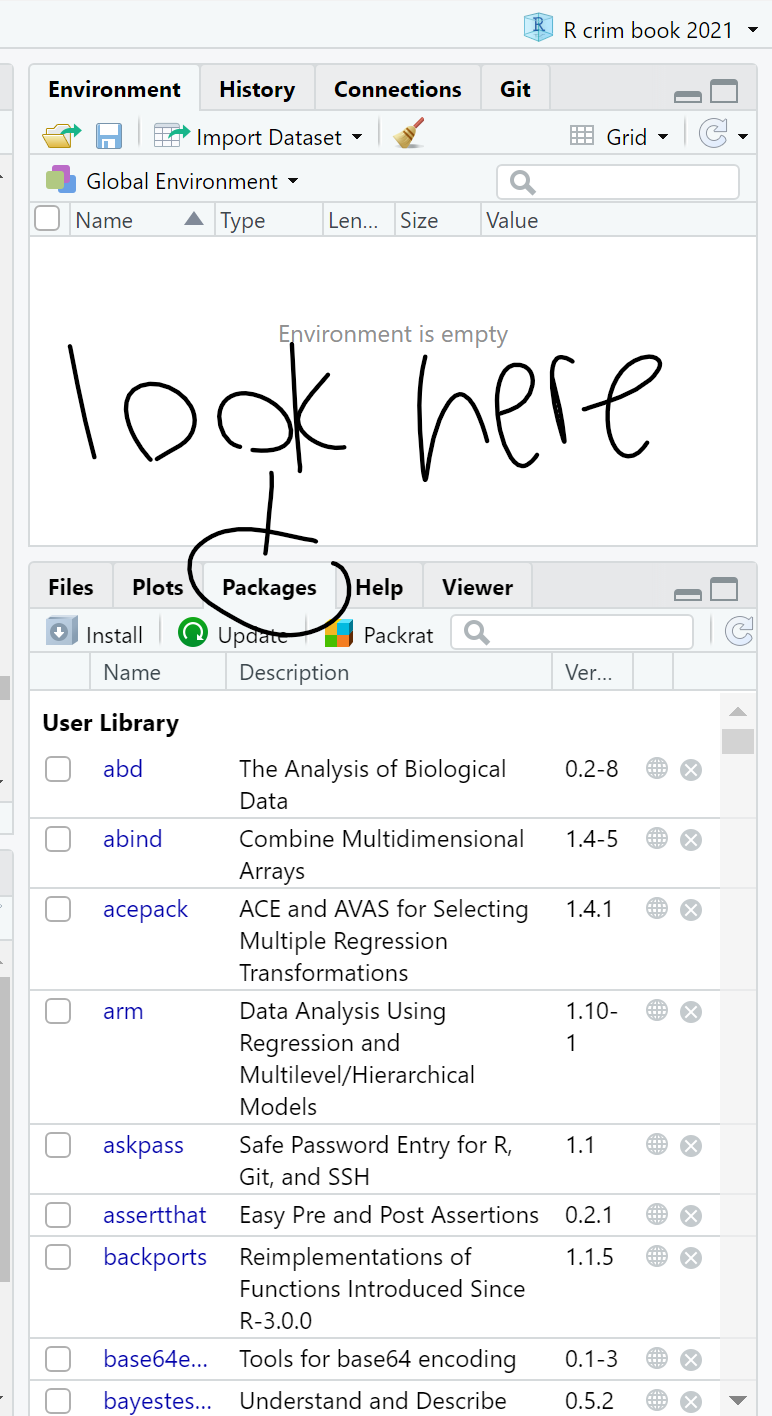
\includegraphics[width=0.35\textwidth,height=\textheight]{Images/packages.png}
\caption{\textbf{Figure 1.14} Packages Tab}
\end{figure}

A number of the packages we will use belong to a set of packages called \textbf{tidyverse}. These packages help make your data tidy. According to Statistician and Chief Scientist at \texttt{RStudio}, Hadley Wickham, (also an author of some of your readings) transforming your data into \emph{tidy data} is one of the most important steps of the data analysis process. It will ensure your data are in the format you need to conduct your analyses.

Packages can be installed using the \texttt{install.packages()} function. Remember that while you only need to install packages once, they need to be loaded with the \texttt{library()}function each time you open up \texttt{RStudio}. Let us install the package \texttt{dplyr} from \texttt{tidyverse} and load it:

\begin{Shaded}
\begin{Highlighting}[]
\FunctionTok{install.packages}\NormalTok{(}\StringTok{"dplyr"}\NormalTok{)}
\end{Highlighting}
\end{Shaded}

\begin{Shaded}
\begin{Highlighting}[]
\FunctionTok{library}\NormalTok{(dplyr)}
\end{Highlighting}
\end{Shaded}

\begin{verbatim}
## 
## Attaching package: 'dplyr'
\end{verbatim}

\begin{verbatim}
## The following objects are masked from 'package:stats':
## 
##     filter, lag
\end{verbatim}

\begin{verbatim}
## The following objects are masked from 'package:base':
## 
##     intersect, setdiff, setequal, union
\end{verbatim}

A lot of code and activity appears in the console. Warnings may manifest. Most of the time, the warnings explain what is being loaded and confirm that the package is successfully loaded. If there is an error, you will have to figure out what the warnings are telling you to successfully load the package. This happens and is normal.

To double check that you have actually installed \texttt{dplyr}, go to that \emph{File Directory, Plots, Packages} pane and click on the \emph{Packages} tab. The list of packages is in alphabetical order and \texttt{dplyr} should be there. If there is a tick in its box, it means that this package is currently loaded and you can use it; if there is no tick, it means that it is inactive, and you will have to bring it up with \texttt{library()}, or just tick its box (Figure 1.15).

\begin{figure}
\centering
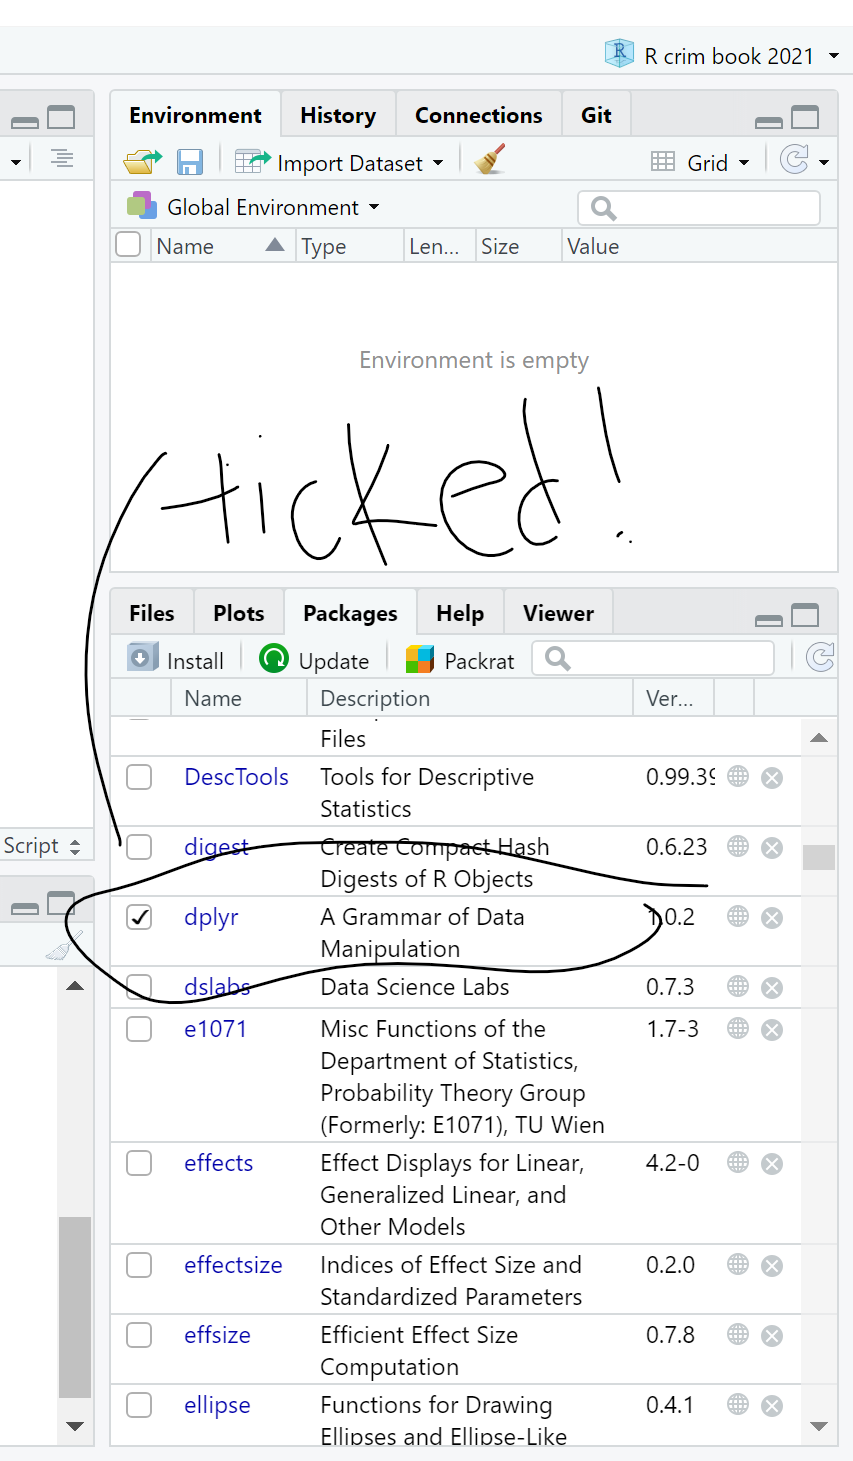
\includegraphics[width=0.35\textwidth,height=\textheight]{Images/dplyr.png}
\caption{\textbf{Figure 1.15} dplyr Package Ticked}
\end{figure}

On \emph{masking}: sometimes packages introduce functions that have the same name as those that are already loaded, maybe from another package, into your session. When that happens, the newly loaded ones will override the previous ones. You can still use them but you will have to refer to them explicitly by bringing them up by specifying to which package they belong using \texttt{library()}.

Keep \texttt{dplyr} in mind as next week we will learn more about it!

\begin{center}\rule{0.5\linewidth}{0.5pt}\end{center}

\hypertarget{summary}{%
\section{SUMMARY}\label{summary}}

Today you installed both \texttt{R} and \texttt{RStudio} and had a gander around the \texttt{RStudio} interface. If you were bored with its default look, you could customise the interface. When working with \texttt{RStudio}, it is best to have the four panes. One had to do with the all-important \textbf{script} and we use \texttt{\#} in the coding when we want to make \textbf{comments}.

We learned about some important features of \texttt{R}. First were the \textbf{operators}. These are symbols that tell \texttt{R} what to do and come in four types. One we will use quite a bit is the \emph{assignment operator}, which is the symbol, \texttt{\textless{}-}. Also important were \textbf{functions}, which are similar to operators except their names tell you what they do. Second were \textbf{objects}, which are pervasive when working with \texttt{R}. They are like boxes that you put stuff in, and we learned about three specific types of \textbf{data structure} objects: vectors, lists, and data frames. Third were \textbf{packages}. These are open source software that expand what \texttt{R} can do. We installed \texttt{dplyr} as an example, and we will use this \texttt{tidyverse} package in our next session.

That is all for today. Do not forget to do your homework task and the quiz by next week!

\hypertarget{getting-to-know-your-data}{%
\chapter{Getting to know your data}\label{getting-to-know-your-data}}

\hypertarget{variables-labels-and-subsetting}{%
\subsubsection*{\texorpdfstring{\emph{Variables, Labels, and Subsetting}}{Variables, Labels, and Subsetting}}\label{variables-labels-and-subsetting}}
\addcontentsline{toc}{subsubsection}{\emph{Variables, Labels, and Subsetting}}

\hypertarget{learning-outcomes-1}{%
\paragraph*{\texorpdfstring{\textbf{Learning Outcomes:}}{Learning Outcomes:}}\label{learning-outcomes-1}}
\addcontentsline{toc}{paragraph}{\textbf{Learning Outcomes:}}

\begin{itemize}
\tightlist
\item
  Create a project in \texttt{R} to refer back to for each session
\item
  Understand what variables are and how to examine them in \texttt{R}
\item
  Learn how to make new variables
\item
  Learn how to label variables and their values
\item
  Learn how to subset select observations and variables
\end{itemize}

\hypertarget{todays-learning-tools-1}{%
\paragraph*{\texorpdfstring{\textbf{Today's Learning Tools:}}{Today's Learning Tools:}}\label{todays-learning-tools-1}}
\addcontentsline{toc}{paragraph}{\textbf{Today's Learning Tools:}}

\hypertarget{total-number-of-activities-9}{%
\paragraph*{\texorpdfstring{\emph{Total number of activities}: 9}{Total number of activities: 9}}\label{total-number-of-activities-9}}
\addcontentsline{toc}{paragraph}{\emph{Total number of activities}: 9}

\hypertarget{data-1}{%
\paragraph*{\texorpdfstring{\emph{Data:}}{Data:}}\label{data-1}}
\addcontentsline{toc}{paragraph}{\emph{Data:}}

\begin{itemize}
\tightlist
\item
  National Crime Victimization Survey (NCVS)
\end{itemize}

\hypertarget{packages-2}{%
\paragraph*{\texorpdfstring{\emph{Packages:}}{Packages:}}\label{packages-2}}
\addcontentsline{toc}{paragraph}{\emph{Packages:}}

\begin{itemize}
\tightlist
\item
  \texttt{dplyr}
\item
  \texttt{here}
\item
  \texttt{haven}
\item
  \texttt{labelled}
\item
  \texttt{sjlabelled}
\end{itemize}

\hypertarget{functions-introduced-and-packages-to-which-they-belong-1}{%
\paragraph*{\texorpdfstring{\emph{Functions introduced (and packages to which they belong)}}{Functions introduced (and packages to which they belong)}}\label{functions-introduced-and-packages-to-which-they-belong-1}}
\addcontentsline{toc}{paragraph}{\emph{Functions introduced (and packages to which they belong)}}

\begin{itemize}
\tightlist
\item
  \texttt{\%\textgreater{}\%} : Known as the pipe operator, and allows users to pass one output of a code to become the input of another ( \texttt{dplyr})
\item
  \texttt{as\_factor()} : Changes the class of an object to factor class (\texttt{haven})
\item
  \texttt{attributes()} : Access object attributes, such as value labels (\texttt{base\ R})
\item
  \texttt{case\_when()} : Allows users to vectorize multiple if / if else statements (\texttt{dplyr})
\item
  \texttt{count()} : Counts the number of occurrences (\texttt{dplyr})
\item
  \texttt{dim()} : Returns the number of observations and variables in a data frame (\texttt{base\ R})
\item
  \texttt{dir.create()} : creates a new folder in a project (\texttt{base\ R})
\item
  \texttt{factor()} Creates a factor (\texttt{base\ R})
\item
  \texttt{filter()} : Subsets a data frame to rows when a condition is true (\texttt{dplyr})
\item
  \texttt{get\_labels()} : Returns value labels of labelled data (\texttt{sjlabelled})
\item
  \texttt{here()} : Finds a project's files based on the current working directory (\texttt{here})
\item
  \texttt{mutate()} : Creates new vectors or transforms existing ones (\texttt{dplyr})
\item
  \texttt{names()} : Returns the names of the variables in the data frame (\texttt{base\ R})
\item
  \texttt{read\_spss()} : Imports SPSS .sav files (\texttt{haven})
\item
  \texttt{recode()} : Substitutes old values of a factor or a numeric vector with new ones (\texttt{dplyr})
\item
  \texttt{remove\_labels()} : Removes value labels from a variable (\texttt{sjlabelled})
\item
  \texttt{remove\_var\_label()} : Removes a variable's label (\texttt{labelled})
\item
  \texttt{select()} : Select columns to retain or drop (\texttt{dplyr})
\item
  \texttt{table()}: Generates a frequency table (\texttt{base\ R})
\item
  \texttt{var\_label()} : Returns or sets a variable label (\texttt{labelled})
\end{itemize}

\begin{center}\rule{0.5\linewidth}{0.5pt}\end{center}

\hypertarget{the-tidyverse}{%
\section{The Tidyverse}\label{the-tidyverse}}

Last time, we installed our first package, \texttt{dplyr}. This is one of a number of packages from what is known as \textbf{tidyverse}.

\begin{figure}
\centering

\includegraphics[width=0.3\textwidth,height=\textheight]{Images/tidyverse-logo.png}
\caption{\textbf{Figure 2.1} Tidyverse logo}
\end{figure}

The tidyverse contains packages that help us carry out \textbf{wrangling} (i.e., cleaning variables), analysis, plotting, and modelling of our data. The ethos of tidyverse is that working and using tidy data makes our lives easier in the long run, allows us to stick to specific conventions, and enables us to share with others who follow this approach. Essentially, tidy data makes data analysis easy to carry out and to communicate to others.

So what is tidy data?

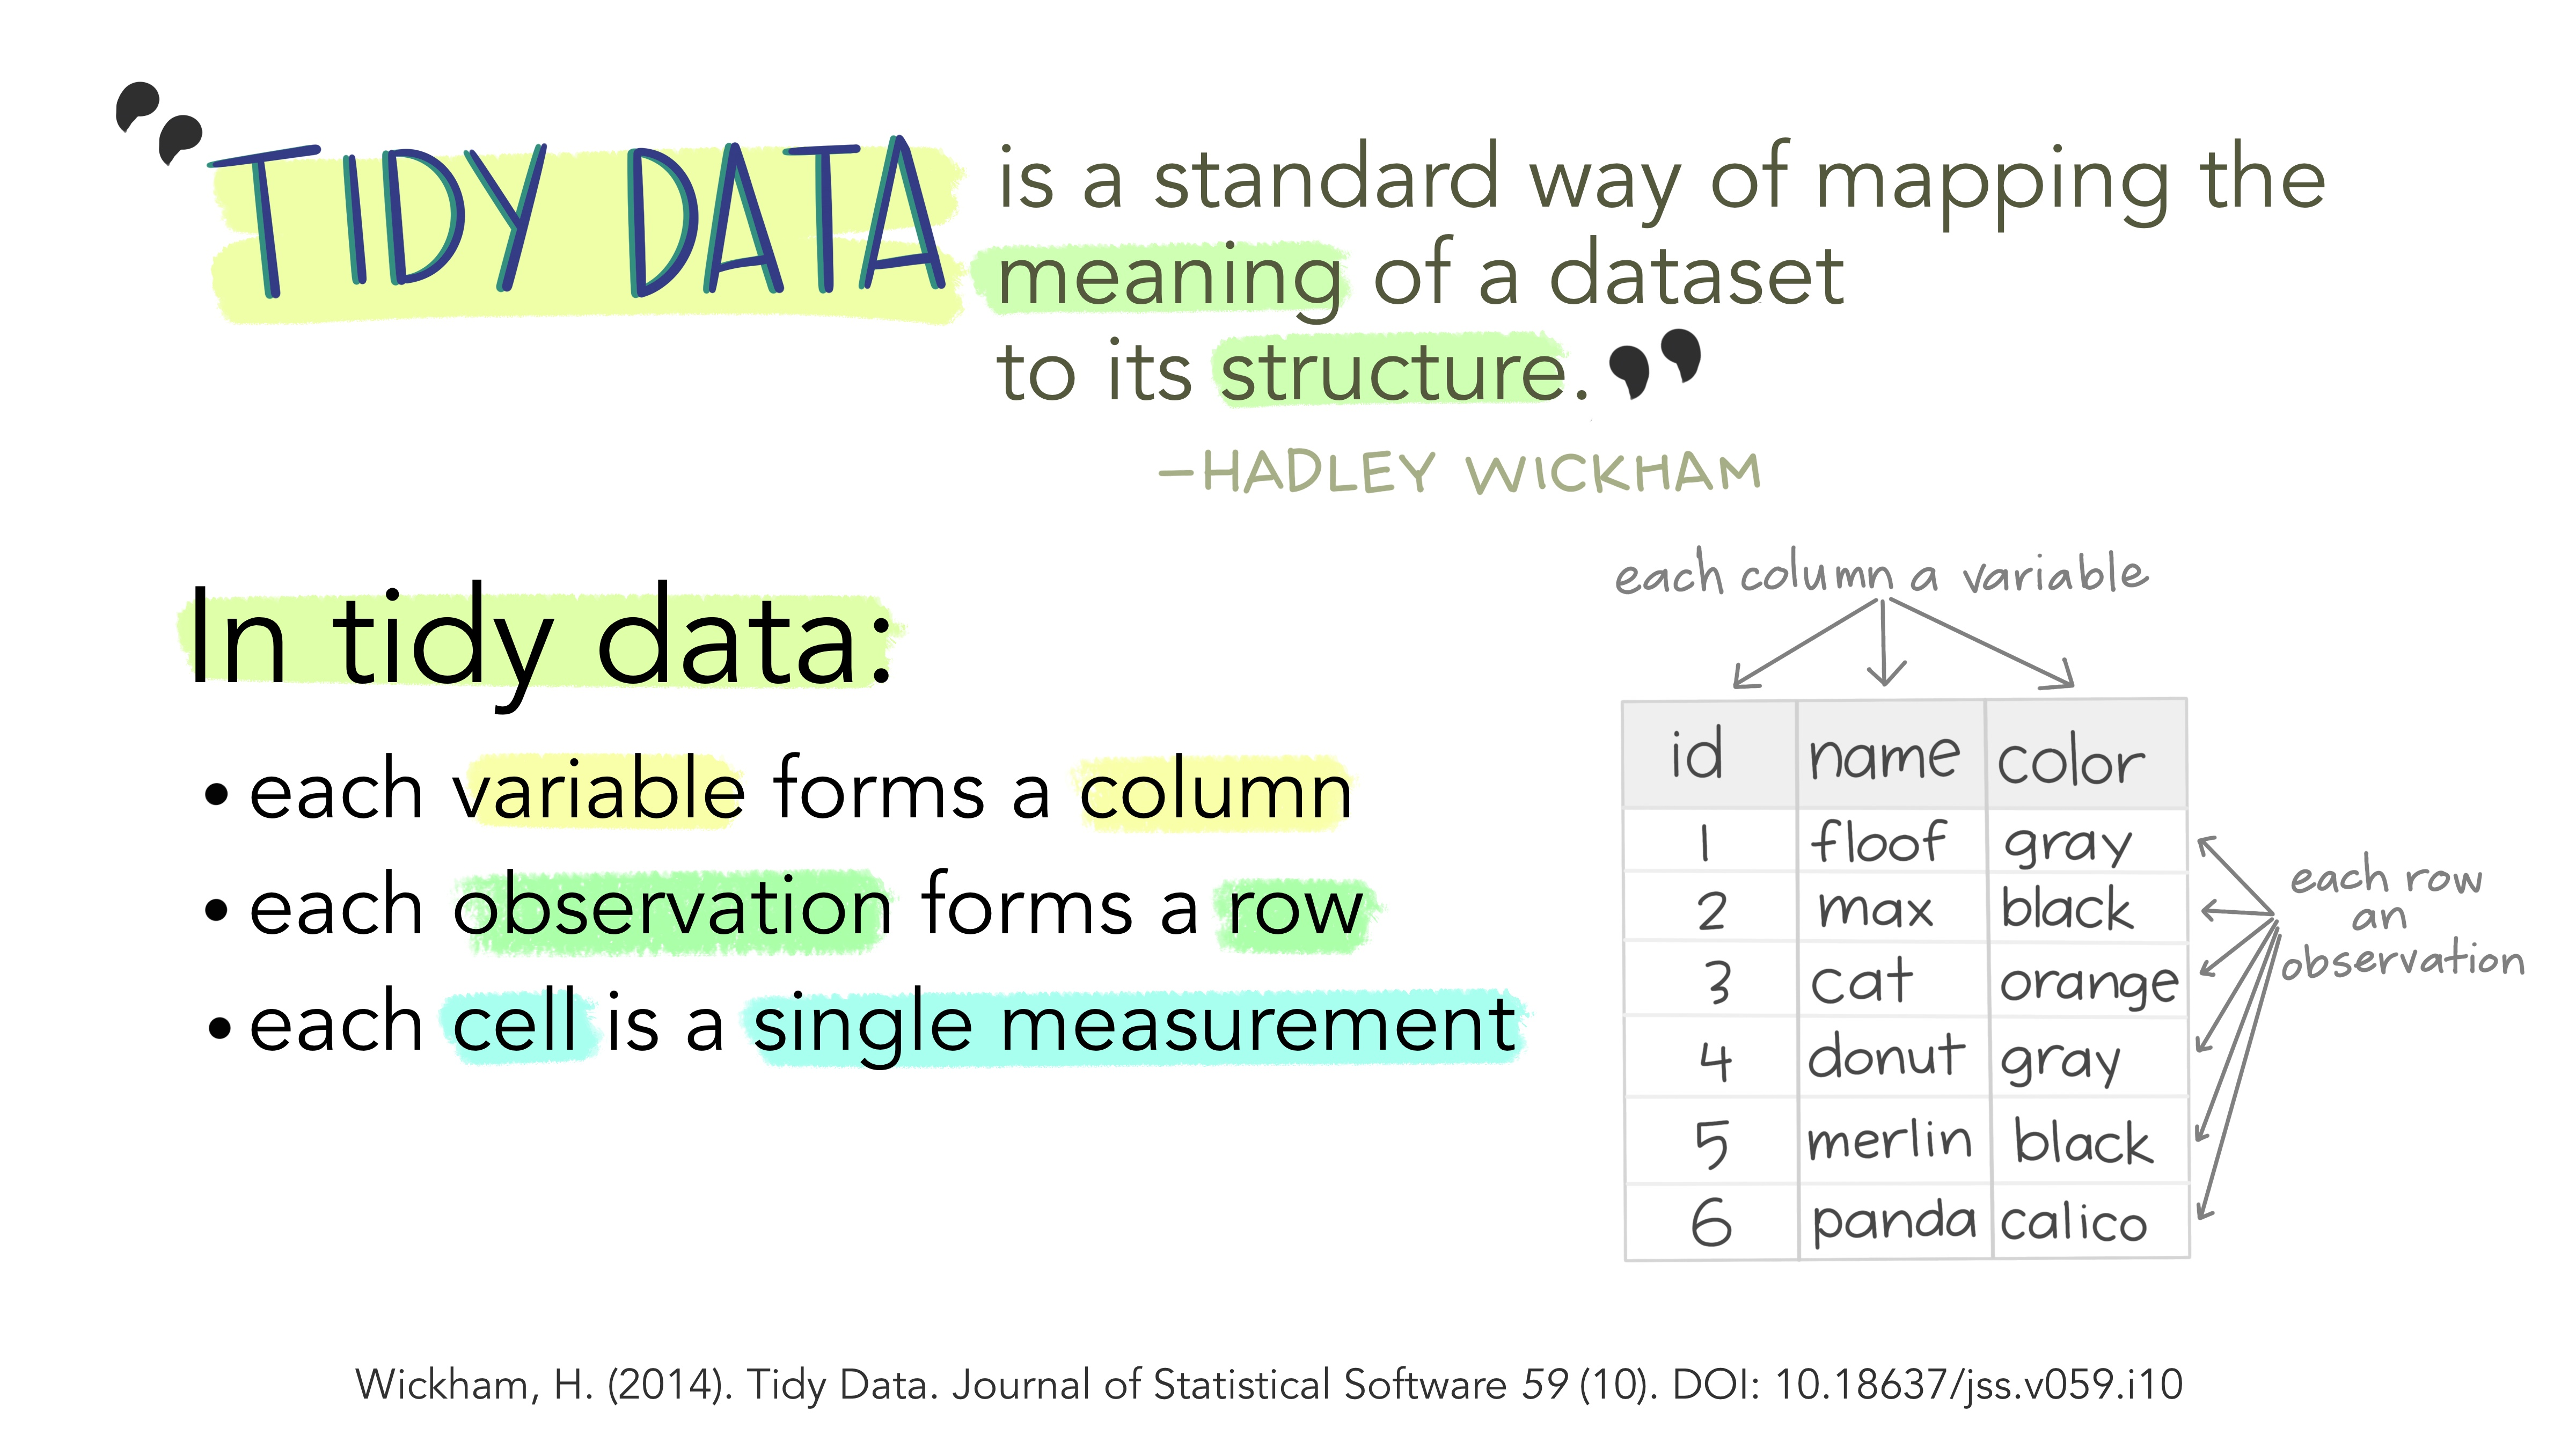
\includegraphics[width=0.8\textwidth,height=\textheight]{Images/tidydata_1.jpg}

Like what was mentioned in last week's lesson, our columns represent our variables, but, also, our cases (or better known in the tidyverse as \textbf{observations}) are our rows, whereby each cell is a value of that column's given variable for the observation in that row.

In this class, we will be working with tidy data. Generally, if you have messy data, which is common in the real world of data analysis, your first task is to wrangle it until it is in a tidy shape similar to the ones described in Figures 2.2 and 2.3.

\begin{figure}
\centering
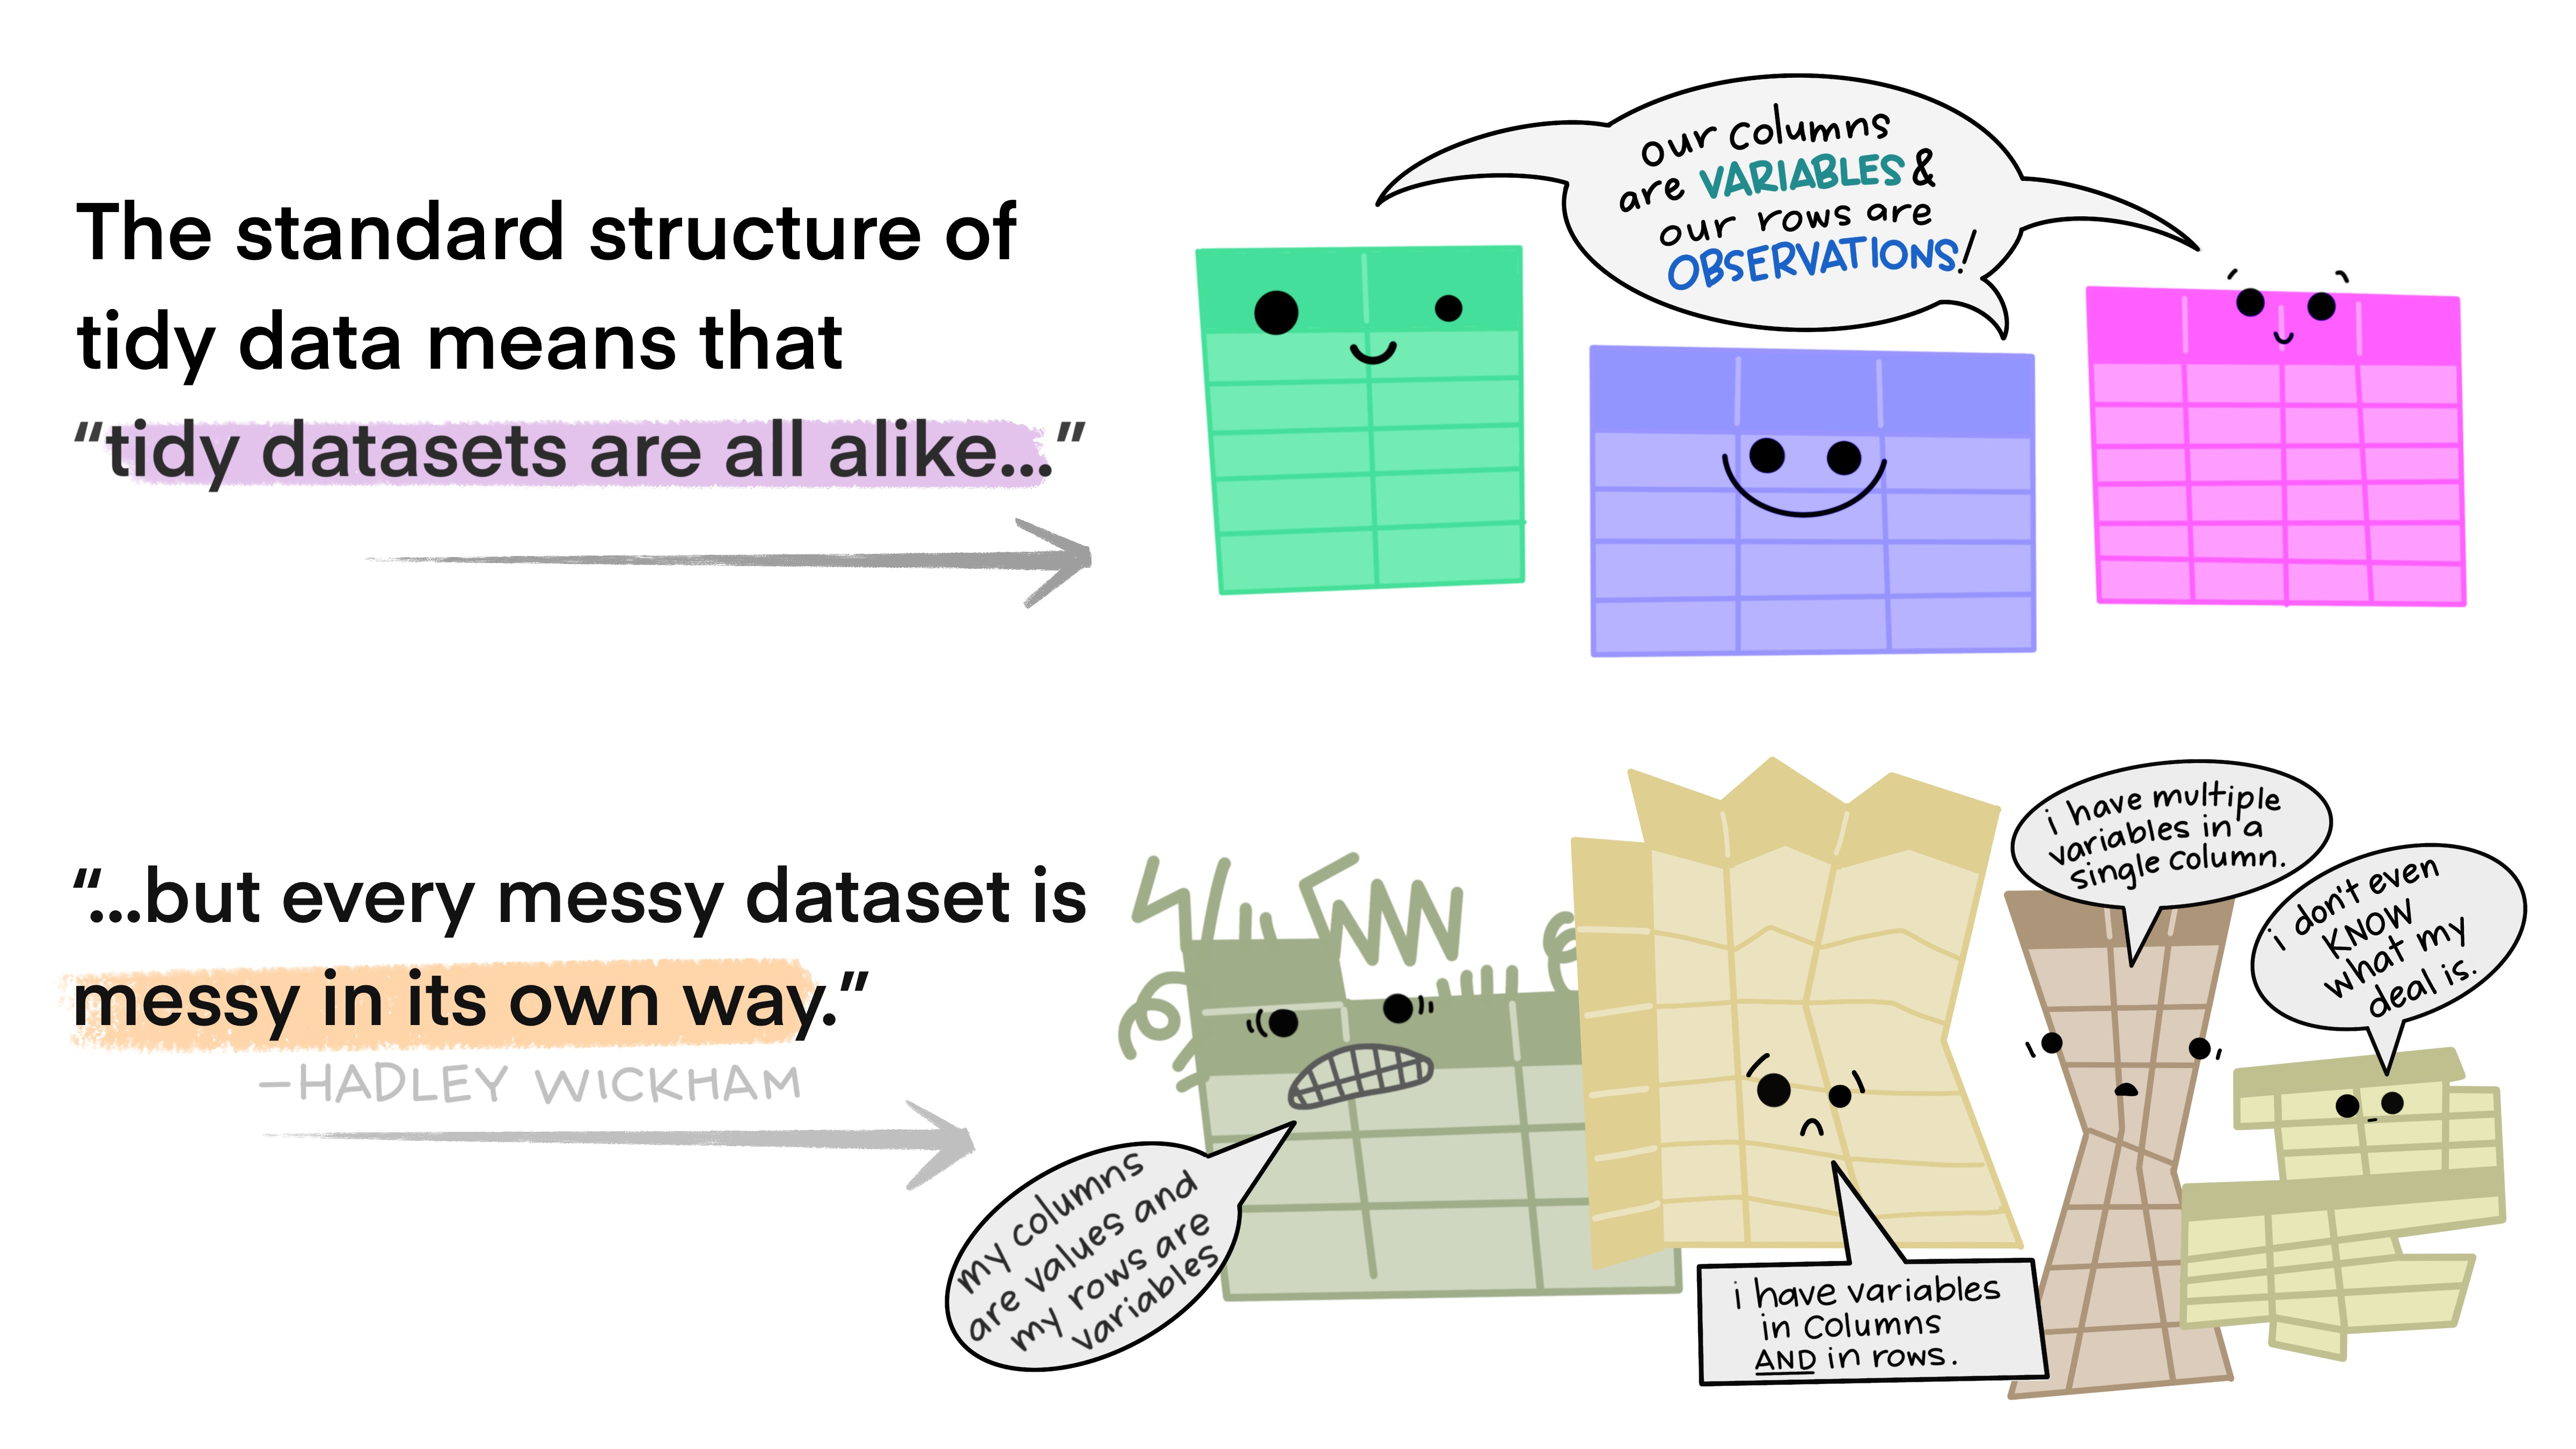
\includegraphics[width=0.8\textwidth,height=\textheight]{Images/tidydata_2.jpg}
\caption{\textbf{Figure 2.3} Tidy data versus messy data by Alison Horst}
\end{figure}

In today's lesson, we use \texttt{dplyr} and other \texttt{tidyverse} packages to explore and get to know our data.

Being familiar with our data requires knowing what they comprise and what form they take. `Tidying' our data through wrangling -- labelling, reformatting, recoding, and creating new variables -- will help with this step in the data analysis process. Today we will learn another three topics related to tidy data: \textbf{variables}, \textbf{labels}, and \textbf{subsetting}.

Let us get started and load \texttt{dplyr}:

\begin{Shaded}
\begin{Highlighting}[]
\FunctionTok{library}\NormalTok{(dplyr)}
\end{Highlighting}
\end{Shaded}

\begin{verbatim}
## 
## Attaching package: 'dplyr'
\end{verbatim}

\begin{verbatim}
## The following objects are masked from 'package:stats':
## 
##     filter, lag
\end{verbatim}

\begin{verbatim}
## The following objects are masked from 'package:base':
## 
##     intersect, setdiff, setequal, union
\end{verbatim}

\begin{Shaded}
\begin{Highlighting}[]
\CommentTok{\# Like last week, you can also check the \textquotesingle{}Packages\textquotesingle{} tab in the \textquotesingle{}Files, Plots...\textquotesingle{} pane to see if the box next to \textquotesingle{}dplyr\textquotesingle{} has been ticked}
\end{Highlighting}
\end{Shaded}

\begin{center}\rule{0.5\linewidth}{0.5pt}\end{center}

\hypertarget{r-projects-getting-your-work-files-organised}{%
\section{R Projects -- Getting Your Work Files Organised}\label{r-projects-getting-your-work-files-organised}}

Although today is focused on tidy data, it is also helpful if whatever you are working on is also tidy and found in one easily accessible folder. By saving work inside a \textbf{project}, you can find files such as data and scripts related to specific work in a single working directory. Let us get into the habit of doing this:

\hypertarget{activity-1-making-yourself-a-project}{%
\subsection{Activity 1: Making yourself a project}\label{activity-1-making-yourself-a-project}}

• Click on the top right tab called \emph{Project: (None)} - Figure 2.4

\begin{figure}
\centering
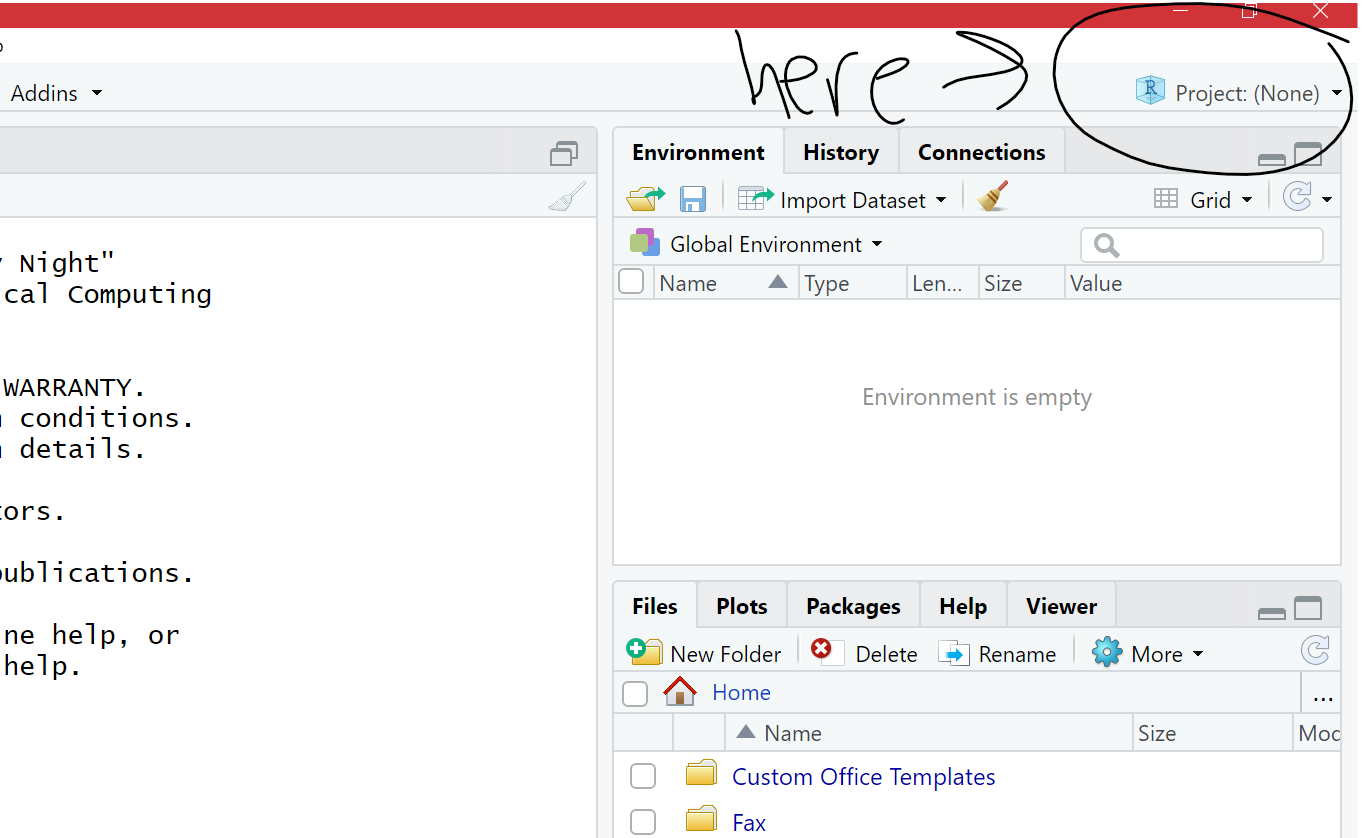
\includegraphics[width=0.5\textwidth,height=\textheight]{Images/project.png}
\caption{\textbf{Figure 2.4} Click on Project: (None)}
\end{figure}

In the options that appear, choose \emph{Existing Directory}. The reason is you may have already created a folder for this work if you had saved your script from last week and from what you have done so far today. For example, Reka had saved a folder called `modelling2021' with her scripts in it and will have her project in that same place too (see Figures 2.5 and 2.6).

\begin{figure}
\centering
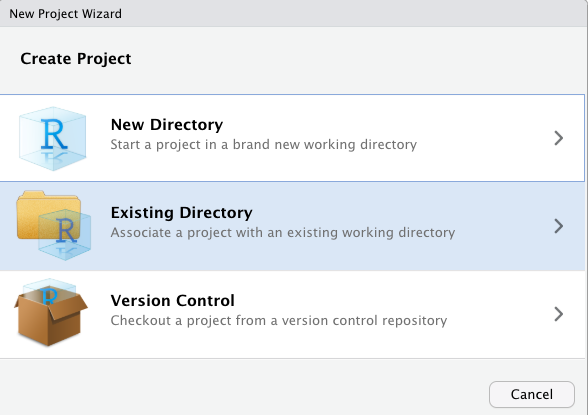
\includegraphics[width=0.5\textwidth,height=\textheight]{Images/existing_dir.png}
\caption{\textbf{Figure 2.5} Existing directory}
\end{figure}

\begin{figure}
\centering
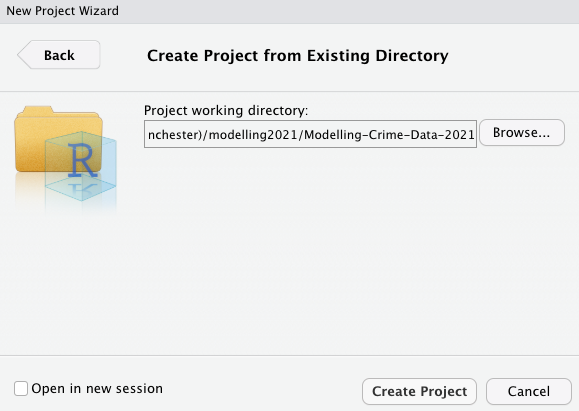
\includegraphics[width=0.5\textwidth,height=\textheight]{Images/browse_proj_dir.png}
\caption{\textbf{Figure 2.6} Create project from existing directory}
\end{figure}

Another option appears (Figure 2.6). Use the `Browse\ldots{}' button to select the folder where you have so far saved your script(s). Once you have done this, click on \emph{Create Project} and your new project will be launched.

This will now open up a new \texttt{RStudio} window with your project. In the future, you can start right where you left off by double clicking your project, which is a \texttt{.Rproj} file, to open it. It helps if you keep all your work for this class in one place, so \texttt{R} can read everything from that folder.

Now if you did not save any scripts or files thus far, so want to create a project in a new place, you can do the following:

\begin{itemize}
\item
  Click on \emph{New Project} (Figure 2.5). A window with different options appears. Create your project in \emph{New Directory} and then click \emph{New Project}
\item
  Choose a name for your project (e.g., r\_crim\_course) and a location (i.e., working directory, which will be explained a little further below) where your project will be created
\end{itemize}

Inside your project, you can organise it by having separate files: one for scripts, one for data, one for outputs, and another for visuals. You can make these with the function \texttt{dir.create()}:

\begin{Shaded}
\begin{Highlighting}[]
\CommentTok{\# For example, to make a sub{-}folder called \textquotesingle{}Datasets\textquotesingle{} in your project folder, type this into your console pane:}
\FunctionTok{dir.create}\NormalTok{(}\StringTok{"Datasets"}\NormalTok{)}
\end{Highlighting}
\end{Shaded}

Another example: to create the online tutorial for this class, we have a project called \texttt{Modelling-Crime-Data-2021}. Figure 2.7 shows that this title appears in the top right hand corner and its contents, including sub-folders, appear in under the \emph{Files} tab in the \emph{Files, Plots\ldots{}} pane.

\begin{figure}
\centering
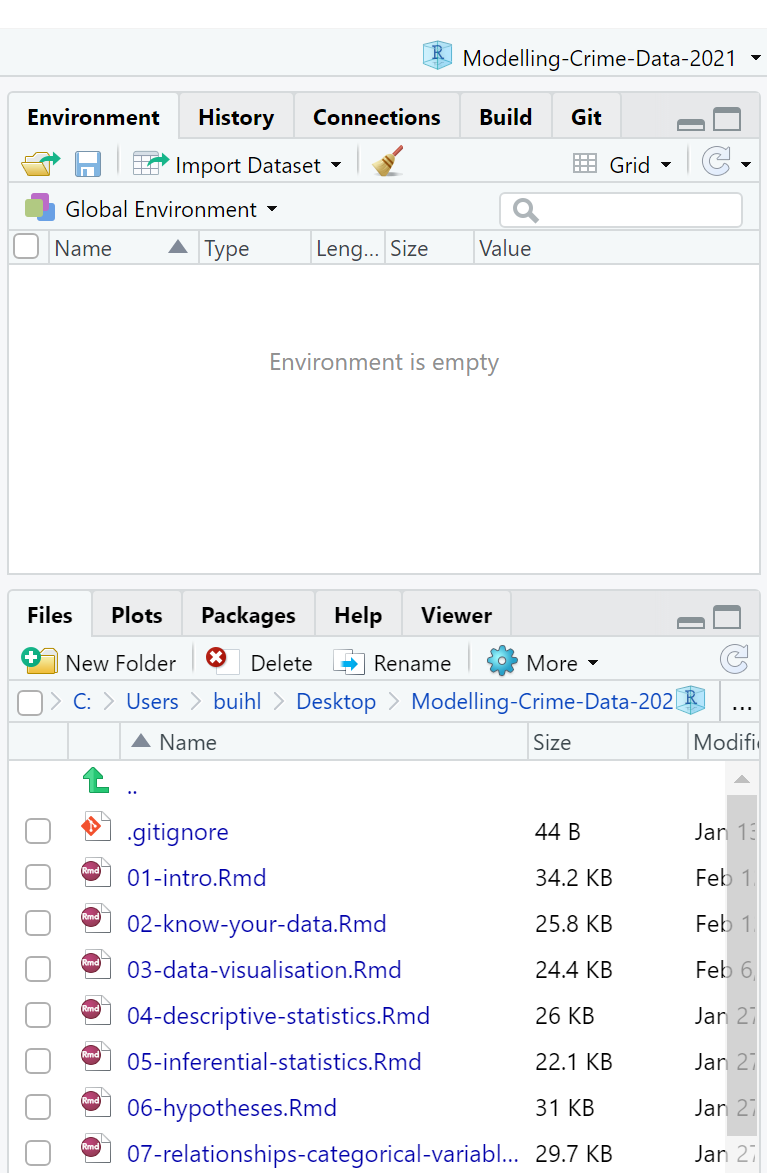
\includegraphics[width=0.4\textwidth,height=\textheight]{Images/project2.png}
\caption{\textbf{Figure 2.7} How a project appears}
\end{figure}

The files in your \emph{Files, Plots\ldots{}} pane tell you in what folder you are automatically working. This is known as your \textbf{working directory}, the default location that appears when you open \texttt{RStudio}. Wherever your \texttt{R\ project} (that file ending in \texttt{.Rproj}) is saved will be the working directory.

In your group google sheets, type the name of your \texttt{R} project and in which location it is in. Now decide whether this is a good location for your \texttt{R} project. For example, is the location name too long? (Something like `C:~Users~xx~Desktop ~xx~xx~Manchester~xx ~xx~xx~xx~xx~xx' is too long and you might run into problems later.) Or are there files that are for your other course units in there too? If doubtful about the location of your project, move it somewhere else you think is more appropriate.

You can read on why projects are useful here: \url{https://www.r-bloggers.com/2020/01/rstudio-projects-and-working-directories-a-beginners-guide/}

\begin{center}\rule{0.5\linewidth}{0.5pt}\end{center}

\hypertarget{the-here-package}{%
\subsubsection{\texorpdfstring{The \texttt{here} package}{The here package}}\label{the-here-package}}

Whenever you want to locate certain files within your Project, use the \texttt{here} package:

\begin{Shaded}
\begin{Highlighting}[]
\CommentTok{\# First, you must install it if you have not done so:}
\FunctionTok{install.packages}\NormalTok{(}\StringTok{"here"}\NormalTok{)}
\end{Highlighting}
\end{Shaded}

\begin{Shaded}
\begin{Highlighting}[]
\CommentTok{\# Then bring it up with \textquotesingle{}library()\textquotesingle{} because it may not come up automatically after installing it}
\FunctionTok{library}\NormalTok{(here)}
\end{Highlighting}
\end{Shaded}

\begin{verbatim}
## here() starts at /Users/reka/Dropbox (The University of Manchester)/modelling2021/Modelling-Crime-Data-2021
\end{verbatim}

Using the \texttt{here} package is better than typing out the exact location of your file, which can be tedious. The next section shows how to use the \texttt{here()} function from said package to import data from the National Crime Victimization Survey (NCVS).

\begin{center}\rule{0.5\linewidth}{0.5pt}\end{center}

\hypertarget{importing-data}{%
\section{Importing Data}\label{importing-data}}

Here is another \texttt{tidyverse} package to install:

\begin{Shaded}
\begin{Highlighting}[]
\FunctionTok{install.packages}\NormalTok{(}\StringTok{"haven"}\NormalTok{)}
\end{Highlighting}
\end{Shaded}

\begin{Shaded}
\begin{Highlighting}[]
\FunctionTok{library}\NormalTok{(haven)}
\end{Highlighting}
\end{Shaded}

\texttt{haven} enables \texttt{R} to understand various data formats used by other statistical packages such as SPSS and STATA. We will need this package to open data in its diverse forms. When we worked with Excel last semester in \emph{Making Sense of Criminological Data}, we could only open certain type of files. With \texttt{R}, we can open a wide range of data files, which opens up many possibilities of analysis for us. Let us give this a try now.

\hypertarget{activity-2-importing-and-viewing-data}{%
\subsection{Activity 2: Importing and Viewing Data}\label{activity-2-importing-and-viewing-data}}

Go to the class Blackboard. Then click on \emph{Learning materials} and then on \emph{Week 2} where you will find the dataset `NCVS lone offender assaults 1992 to 2013'.

Download the data into the \emph{Datasets} sub-folder in your working directory you had created using the function \texttt{dir.create()}.

This data comes from The National Crime Victimization Survey (NCVS) from the US. You can read more about it \href{https://www.bjs.gov/index.cfm?ty=dcdetail\&iid=245}{here}.

Now how to bring this dataset up in \texttt{RStudio}? We must follow these steps to \emph{read} the data:

\begin{itemize}
\item
  \begin{enumerate}
  \def\labelenumi{\arabic{enumi}.}
  \tightlist
  \item
    We note what kind of dataset file, `NCVS lone offender assaults 1992 to 2013', is. The extension is \texttt{.sav} and this means that it is a file from the statistical package SPSS, so the function we need is \texttt{read\_spss()} from the \texttt{haven} package.
  \end{enumerate}
\end{itemize}

\begin{itemize}
\item
  \begin{enumerate}
  \def\labelenumi{\arabic{enumi}.}
  \setcounter{enumi}{1}
  \tightlist
  \item
    When importing data with the \texttt{here()} function, you must specify where the file is and what it is called in the brackets. In this case, we need to specify that it is in the sub-folder `Datasets' and it is called `NCVS lone offender assaults 1992 to 2013.sav'. So, the code to find the file would be: \texttt{here("Datasets",\ "NCVS\ lone\ offender\ assaults\ 1992\ to\ 2013.sav")}.
  \end{enumerate}
\end{itemize}

Completing these steps, we now can load our dataset and place it inside a data frame called \texttt{ncvs}:

\begin{Shaded}
\begin{Highlighting}[]
\CommentTok{\# Importing our SPSS dataset and naming it ‘ncvs’ }
\NormalTok{ncvs }\OtherTok{\textless{}{-}} \FunctionTok{read\_spss}\NormalTok{(}\FunctionTok{here}\NormalTok{(}\StringTok{"Datasets"}\NormalTok{, }\StringTok{"NCVS lone offender assaults 1992 to 2013.sav"}\NormalTok{))}
\end{Highlighting}
\end{Shaded}

What you are saying to \texttt{R} is the following:

\begin{quote}
My data, \emph{NCVS lone offender assaults 1992 to 2013}, is a .sav file. Therefore, it is an SPSS dataset and is located in the sub-folder called \emph{Datasets} in my default working directory. \texttt{R}, please extract it from \emph{here}, understand it, and place it in a data frame object called \texttt{ncvs}, so I can find it in \texttt{RStudio}.
\end{quote}

To view the new data frame, \texttt{ncvs}, type:

\begin{Shaded}
\begin{Highlighting}[]
\FunctionTok{View}\NormalTok{(ncvs)}
\end{Highlighting}
\end{Shaded}

A tab appears labelled `ncvs'. In it, you can view all its contents. In your group google sheets, type how many `entries' and `columns' there are in our data frame, \texttt{ncvs}.

There are other ways to load data that are of different formats. For more information, see \href{https://evoldyn.gitlab.io/evomics-2018/ref-sheets/R_data-import.pdf}{this cheatsheet for importing data}. But for now, you can rely on us showing you the functions you need.

\begin{center}\rule{0.5\linewidth}{0.5pt}\end{center}

\hypertarget{todays-3-topics-1}{%
\section{Today's 3 (TOPICS)}\label{todays-3-topics-1}}

We now have data to tidy in \texttt{R}, so onto our three main topics for this week: \textbf{variables}, \textbf{labels}, and \textbf{subsetting}.

\hypertarget{variables}{%
\subsection{Variables}\label{variables}}

Variables can be persons, places, things, or ideas that we are interested in studying. For example, height and favourite football team.

Last week, we learned a little on how to examine what our variables are. Let us revisit this. One of the first things we do to get to know our \texttt{ncvs} data frame is to identify the number of rows and columns by using the function \texttt{View()} as we did above, or, a more direct way, the function \texttt{dim()}:

\begin{Shaded}
\begin{Highlighting}[]
\FunctionTok{dim}\NormalTok{(ncvs)}
\end{Highlighting}
\end{Shaded}

\begin{verbatim}
## [1] 23969    47
\end{verbatim}

Like your answer from Activity 2, the data frame\texttt{ncvs} has 47 columns, meaning that it has 47 variables. What are these variables all called? We can get their names using the \texttt{names} function:

\begin{Shaded}
\begin{Highlighting}[]
\FunctionTok{names}\NormalTok{(ncvs)}
\end{Highlighting}
\end{Shaded}

\begin{verbatim}
##  [1] "YEAR"                "V2119"               "V2129"              
##  [4] "V3014"               "V3016"               "V3018"              
##  [7] "V3021"               "V3023"               "V3023A"             
## [10] "V3024"               "V2026"               "V4049"              
## [13] "V4234"               "V4235"               "V4236"              
## [16] "V4237"               "V4237A"              "V4238"              
## [19] "V4239"               "V4240"               "V4241"              
## [22] "V4242"               "V4243"               "V4244"              
## [25] "V4245"               "V4246"               "V4246A"             
## [28] "V4246B"              "V4246C"              "V4246E"             
## [31] "V4246F"              "V4246G"              "V4247"              
## [34] "V4528"               "injured"             "privatelocation"    
## [37] "reportedtopolice"    "weaponpresent"       "medicalcarereceived"
## [40] "filter_$"            "relationship"        "Policereported"     
## [43] "victimreported"      "thirdpartyreport"    "maleoff"            
## [46] "age_r"               "vic18andover"
\end{verbatim}

We observe that a number of these variable names are codes, which is somewhat similar to the Crime Survey of England and Wales (CSEW) data we worked with last semester, whereby the variable \emph{polatt7}, for example, was trust in police.

You could view the data frame like you did previously (with the function \texttt{View()}) to find out what the variables actually are, or you could look it up in the data dictionary \href{https://www.icpsr.umich.edu/web/ICPSR/series/95/variables}{here}. The advantage of the data dictionary -- which will accompany all well-documented datasets -- is it will tell you precisely what the variables are and how they measure their characteristics in that particular dataset. For example, the data dictionary that accompanies the NCVS tells us that the variable \texttt{V3014} is age.

\hypertarget{measurement}{%
\subsubsection*{Measurement}\label{measurement}}
\addcontentsline{toc}{subsubsection}{Measurement}

What about the level of measurement for these variables? Different variable types refer to different levels of measurement.

For \textbf{categorical variables}, we can have variables that are nominal (no order), ordinal (have an order), or binary (only two possible options, like `yes' and `no').

\begin{figure}
\centering
\includegraphics[width=0.7\textwidth,height=\textheight]{Images/nominal_ordinal_binary.png}
\caption{\textbf{Figure 2.8} Categorial variables by Allison Horst}
\end{figure}

\textbf{Numeric variables} can be classified two separate ways. Last semester, we discussed the difference between \emph{interval} and \emph{ratio} variables. Interval variables have the same distance between observations, but have no true zero. The temperature in Celsius is one example. Ratio variables, on the other hand, do have a true zero point. Calculating a ratio from the values of these variables makes sense, but for values from interval variables, it does not. For example, it is pretty meaningless to state that 20 degrees Celsius is twice as hot as 10 degrees Celsius (`0' in Celsius is not the absolute lowest temperature). But if Reka has £30 pounds in her bank account and Laura has £60, it is meaningful to say Laura has twice as much savings as Reka does.

Another way to classify numeric variables is to distinguish between discrete and continuous variables. \emph{Discrete} numeric variables have set values that make sense. For example, crime is one such variable. It is understandable to have 30 burglaries in May and 50 burglaries in December, but it is not understandable to have 45.2482 burglaries. \emph{Continuous} numeric variables, however, can take on any value between a lower and upper bound and be meaningful. For example, weight and height. Here is an apt illustration:

\begin{figure}
\centering
\includegraphics[width=0.7\textwidth,height=\textheight]{Images/continuous_discrete.png}
\caption{\textbf{Figure 2.9} Discrete versus continuous numeric variables by Allison Horst}
\end{figure}

\hypertarget{variables-in-r}{%
\subsubsection{\texorpdfstring{Variables in \texttt{R}}{Variables in R}}\label{variables-in-r}}

So, how are these levels of measurement among variables relevant in \texttt{R}? Nominal and ordinal variables are encoded as a \textbf{factor} class because they are categorical characteristics, so take on a limited number of values; factors are like the integer vector introduced last week but each integer is a label. Numeric variables, on the other hand, are encoded as a \textbf{numeric} class.

\hypertarget{activity-3-identifying-a-variables-level-of-measurement}{%
\paragraph{Activity 3: Identifying a variable's level of measurement}\label{activity-3-identifying-a-variables-level-of-measurement}}

Identifying the level of measurement should be straightforward when examining each variable. In some cases, however, \texttt{R} may not quite grasp what kind of variable you are working with. Thus, you will need to find out what \texttt{R} thinks your variable is classed as.

How do you ask \texttt{R} what your variable is? Let us find out by using our \texttt{ncvs} data frame.

First, do you remember from last week how to refer to one specific variable in your data frame?

It is: \texttt{dataframe\$variablename}

If we want to find out about the variable \texttt{injured} (whether the person was injured or not) from our data frame \texttt{ncvs}, for example, we can refer to the variable specifically. Let us use the \texttt{attributes()} function to examine this variable.

\begin{Shaded}
\begin{Highlighting}[]
\CommentTok{\# To see the class of a specific variable, such as the variable ‘injured’, we use:}
\FunctionTok{attributes}\NormalTok{(ncvs}\SpecialCharTok{$}\NormalTok{injured)}
\end{Highlighting}
\end{Shaded}

\begin{verbatim}
## $label
## [1] "Victim Sustained Injuries During Vicitmization"
## 
## $format.spss
## [1] "F8.2"
## 
## $display_width
## [1] 10
## 
## $class
## [1] "haven_labelled" "vctrs_vctr"     "double"        
## 
## $labels
## uninjured   injured 
##         0         1
\end{verbatim}

\begin{Shaded}
\begin{Highlighting}[]
\CommentTok{\# The $ symbol allows us to access specific variables in a data frame object}

\CommentTok{\# The $ symbol must be accompanied by the name of the data frame!}
\end{Highlighting}
\end{Shaded}

We can see the label (`Victim Sustained Injuries During Vicitmization'), and the values (at the bottom) indicating `0' for `uninjured' and `1' for `injured'. This appears to be a categorical variable with 2 possible values; therefore, a \emph{binary} variable.

Now your turn: find out what is the class of the variable \texttt{weaponpresent}. In your googledoc, type out the answer and the code you used to get that answer.

\begin{center}\rule{0.5\linewidth}{0.5pt}\end{center}

\hypertarget{formatting-classes-and-value-labels}{%
\subsubsection{Formatting Classes and Value Labels}\label{formatting-classes-and-value-labels}}

In some cases, you may want to make changes to how variables are classed. For example, in our data frame \texttt{nvcs}, some of the variables are classed as \texttt{haven\_labelled}.

What is this, you ask? When we use the \texttt{haven()} function to import data, \texttt{R} keeps the information associated with that file -- specifically the value labels that were in the dataset. In practice, therefore, you can find categorical data in \texttt{R} embedded in very different types of vectors (e.g., character, factor, or haven labelled) depending on decisions taken by whomever created the data frame.

Although we understand why these variables are labelled as \texttt{haven\_labelled}, they do not help us understand what class these variables actually are. If we know a variable is classed as factor, We can change it to be so. For example, we want to change the class of variable \texttt{V3018} to be accurately classed as factor:

\begin{Shaded}
\begin{Highlighting}[]
\CommentTok{\# V3018 is a binary variable indicating sex}
\FunctionTok{attributes}\NormalTok{(ncvs}\SpecialCharTok{$}\NormalTok{V3018)}
\end{Highlighting}
\end{Shaded}

\begin{verbatim}
## $label
## [1] "SEX (ALLOCATED)"
## 
## $format.spss
## [1] "F1.0"
## 
## $display_width
## [1] 7
## 
## $class
## [1] "haven_labelled" "vctrs_vctr"     "double"        
## 
## $labels
##            Male          Female         Residue Out of universe 
##               1               2               8               9
\end{verbatim}

\begin{Shaded}
\begin{Highlighting}[]
\CommentTok{\# It is indeed classed as \textquotesingle{}haven{-}labelled\textquotesingle{}}

\CommentTok{\# Naming the newly created factor \textquotesingle{}sex\textquotesingle{} so we do not erase the original variable}
\CommentTok{\# Specify the order we want our variable labels using \textquotesingle{}labels= c()\textquotesingle{}}
\NormalTok{ncvs}\SpecialCharTok{$}\NormalTok{sex }\OtherTok{\textless{}{-}} \FunctionTok{factor}\NormalTok{(ncvs}\SpecialCharTok{$}\NormalTok{V3018, }\AttributeTok{labels =} \FunctionTok{c}\NormalTok{(}\StringTok{"male"}\NormalTok{, }\StringTok{"female"}\NormalTok{))}

\FunctionTok{table}\NormalTok{(ncvs}\SpecialCharTok{$}\NormalTok{sex)}
\end{Highlighting}
\end{Shaded}

\begin{verbatim}
## 
##   male female 
##  12533  11436
\end{verbatim}

\begin{Shaded}
\begin{Highlighting}[]
\FunctionTok{attributes}\NormalTok{(ncvs}\SpecialCharTok{$}\NormalTok{sex)}
\end{Highlighting}
\end{Shaded}

\begin{verbatim}
## $levels
## [1] "male"   "female"
## 
## $class
## [1] "factor"
\end{verbatim}

The new variable, \texttt{sex}, a duplicate of \texttt{V3018}, is no longer a `haven\_labelled' type variable. It is now classed as a factor. But remember, `class' and `factor' are \texttt{R} lingo -- \textbf{we would still describe this as a categorical, binary variable!} We include \texttt{R} language so that you know what it means and how it links to what you have learned in your data analysis classes.

\hypertarget{recoding-and-creating-new-variables}{%
\subsubsection{Recoding and Creating New Variables}\label{recoding-and-creating-new-variables}}

What if we want to create a new variable? Here are three scenarios where we would want to do so:

\emph{Scenario 1}: we want a variable like the \texttt{injured} variable, but for the values, we instead want to see `uninjured' and `injured' and not `0' and `1';

\emph{Scenario 2}: we want a composite variable, like the fear of crime composite variable from last semester that comprised many different scores;

\emph{Scenario 3}: we want to change an existing variable that is \emph{ordinal} with four outcomes into a \emph{binary} variable with only two outcomes.

We address all three scenarios in turn. Recoding and creating new variables is called \textbf{data wrangling} and the package \texttt{dplyr} is most appropriate for doing so.

\begin{figure}
\centering
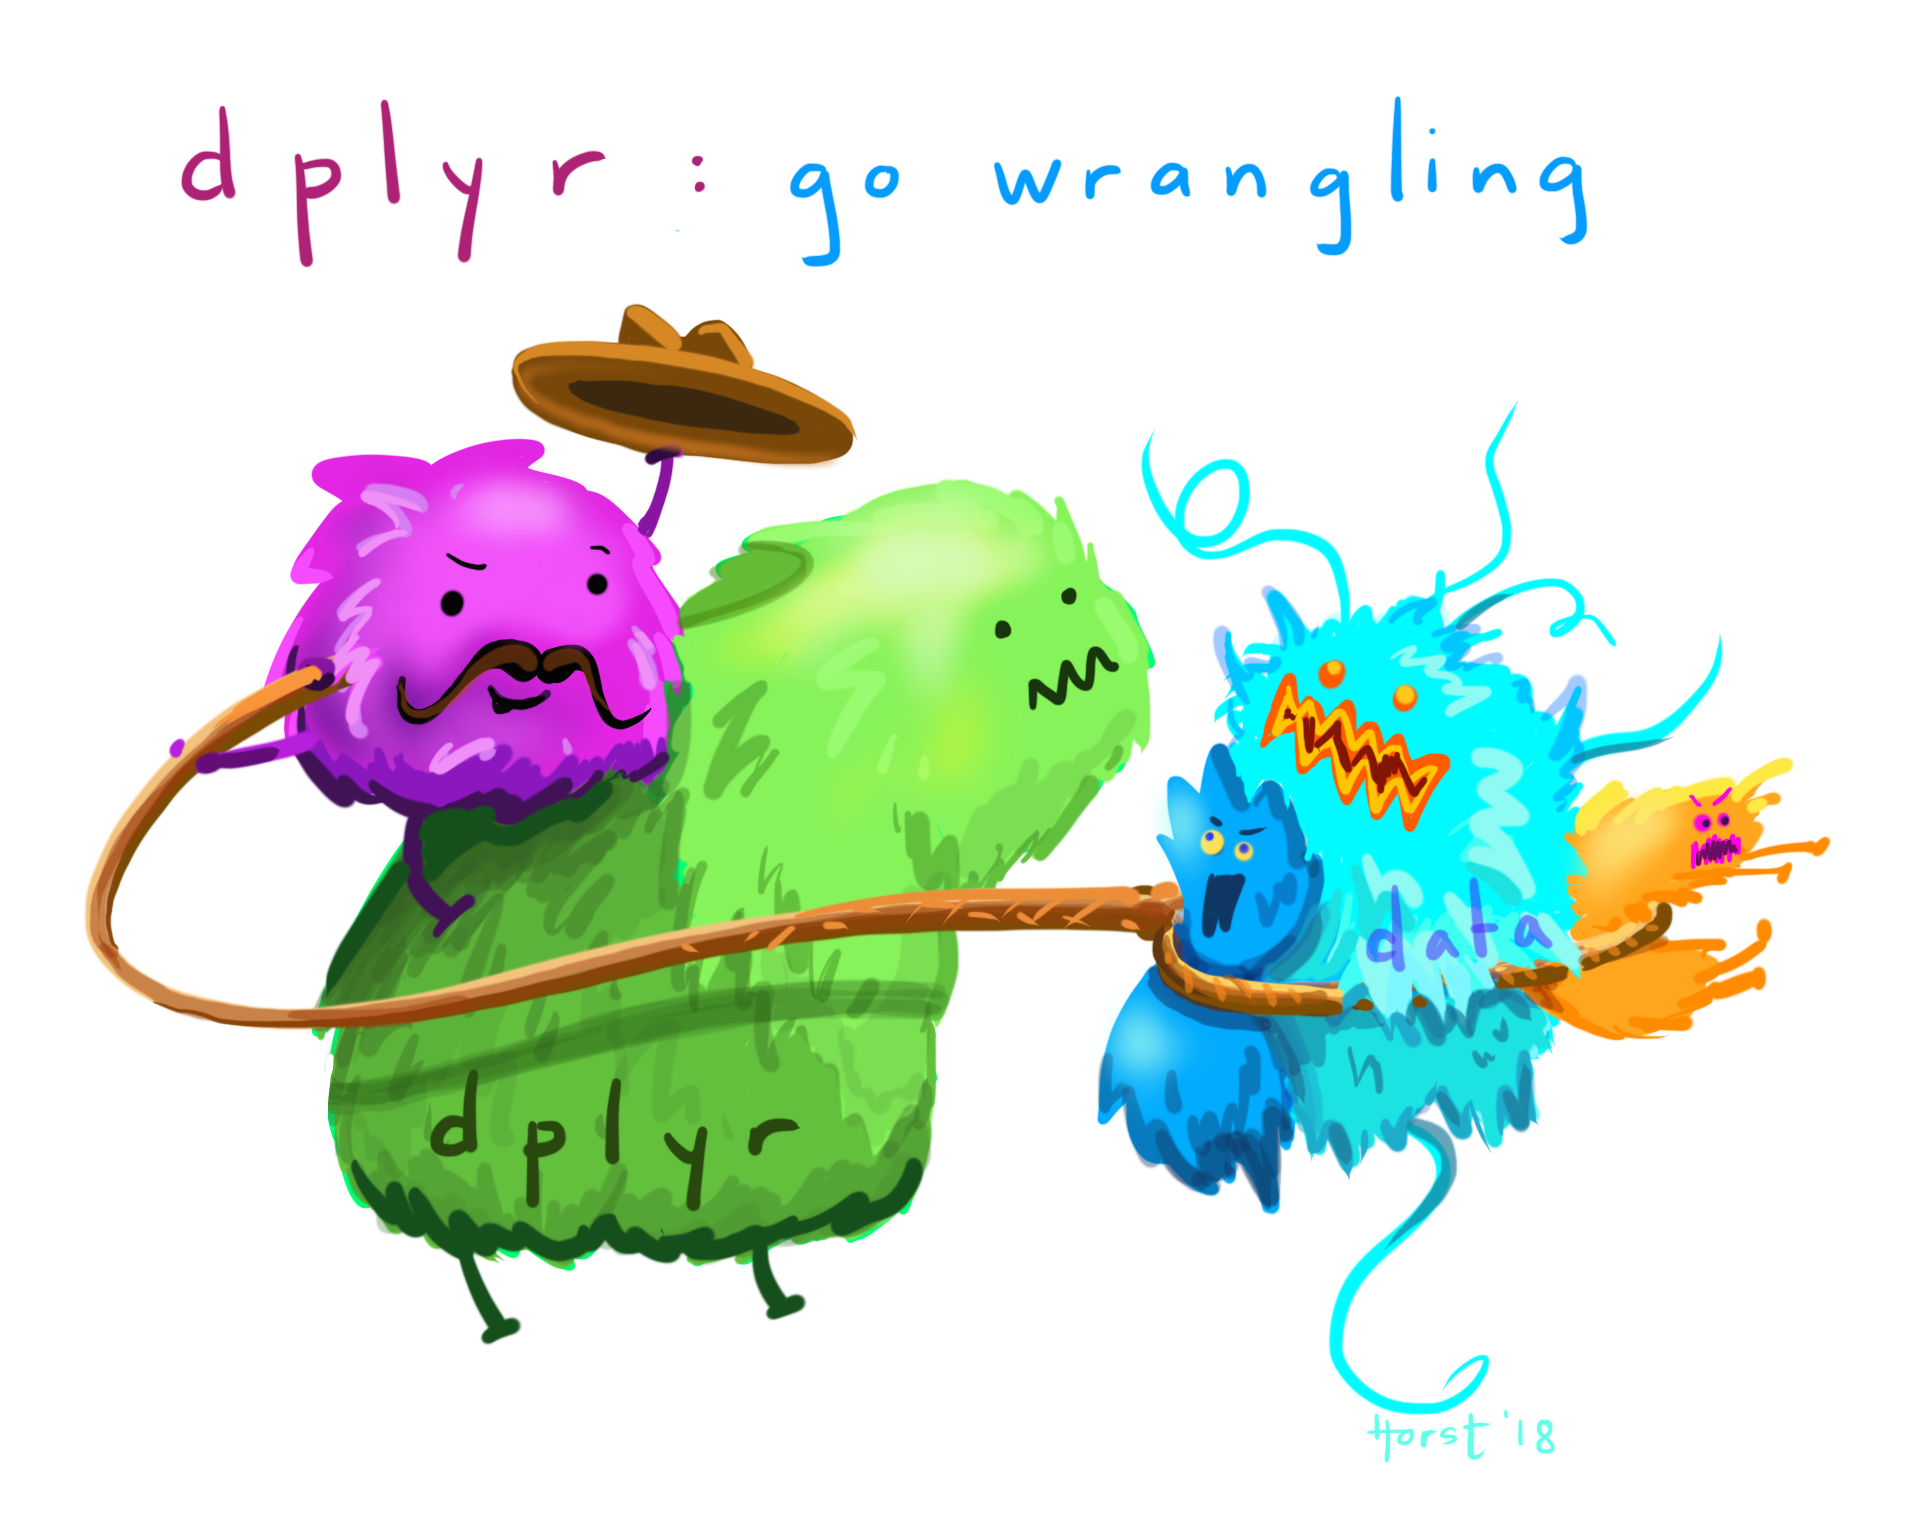
\includegraphics[width=0.7\textwidth,height=\textheight]{Images/dplyr_wrangling.png}
\caption{\textbf{Figure 2.9} Data wrangling by Allison Horst}
\end{figure}

\begin{center}\rule{0.5\linewidth}{0.5pt}\end{center}

\hypertarget{activity-4-creating-a-new-variable-by-recoding-an-existing-one}{%
\subsubsection{Activity 4: Creating a new variable by recoding an existing one}\label{activity-4-creating-a-new-variable-by-recoding-an-existing-one}}

For scenario 1, we want to recode our existing \texttt{injured} variable. We view a frequency table of this variable to understand why. The frequency table tells us the number of times each value for the variable occurs. This is similar to the Pivot Table function in Excel from last semester.

In \texttt{R}, the way to create a frequency table for one variable is to use the function \texttt{table()}. Inside the brackets, you would type the data frame and the variable you want to create the frequency table for. We want a frequency table for the \texttt{injured} variable:

\begin{Shaded}
\begin{Highlighting}[]
\FunctionTok{table}\NormalTok{(ncvs}\SpecialCharTok{$}\NormalTok{injured)}
\end{Highlighting}
\end{Shaded}

\begin{verbatim}
## 
##     0     1 
## 16160  7809
\end{verbatim}

The frequency table shows that 16,160 people answered `0' to the question of whether they were injured, while 7,809 answered `1'. Since we ran our \texttt{attribute()} function earlier, we know that `0' means `uninjured', and `1' means `injured'. Often in data, `0' represents the absence of the feature being measured and `1' means the presence of such feature.

Although we know what the numbers represent, we might forget or someone else unfamiliar with the data views the variable and may not know what the values mean. In this case, it would be helpful to change the numbers `0' and `1' to what they represent.

To do so, we create a new variable whereby a new column appears in the data frame. It is similar to when you create an object. Remember:

\begin{Shaded}
\begin{Highlighting}[]
\NormalTok{name }\OtherTok{\textless{}{-}} \StringTok{"Reka"}
\end{Highlighting}
\end{Shaded}

The only difference is that we must attach this new object (which appears as a column) to the dataframe, and that the number of things we put in this object needs to match the number of rows in that data frame. As we are creating a new variable from one that already has the same number of rows, this is not an issue.

Let us again create a duplicate variable of the \texttt{injured} variable:

\begin{Shaded}
\begin{Highlighting}[]
\CommentTok{\# Create the new variable ‘injured\_new’ from ‘injured’ }
\NormalTok{ncvs}\SpecialCharTok{$}\NormalTok{injured\_new }\OtherTok{\textless{}{-}}\NormalTok{ncvs}\SpecialCharTok{$}\NormalTok{injured }
\end{Highlighting}
\end{Shaded}

View the \texttt{ncvs} data frame. Notice that a new column, \texttt{injured\_new}, appeared at the end with the exact same contents as the variable \texttt{injured}. We will now change those `0' and `1' values.

A function to change values is \texttt{as\_factor()} from the \texttt{haven} package. This function takes the labels assigned to the values of the variable, and changes those original values into these very labels.

\begin{Shaded}
\begin{Highlighting}[]
\CommentTok{\# Remember: You can check what package each function we learn today belongs to by referring to the top of each online lesson, under \textquotesingle{}Functions Introduced\textquotesingle{}}

\NormalTok{ncvs}\SpecialCharTok{$}\NormalTok{injury\_r }\OtherTok{\textless{}{-}} \FunctionTok{as\_factor}\NormalTok{(ncvs}\SpecialCharTok{$}\NormalTok{injured)}
\end{Highlighting}
\end{Shaded}

In the data frame \texttt{ncvs}, you will see this new column \texttt{injured\_r}. If we make the frequency table with this new variable, we see that the values are readily understandable as `uninjured' and `injured':

\begin{Shaded}
\begin{Highlighting}[]
\FunctionTok{table}\NormalTok{(ncvs}\SpecialCharTok{$}\NormalTok{injury\_r)}
\end{Highlighting}
\end{Shaded}

\begin{verbatim}
## 
## uninjured   injured 
##     16160      7809
\end{verbatim}

This a lot easier than `VLOOKUP' from last semester!

\begin{center}\rule{0.5\linewidth}{0.5pt}\end{center}

\hypertarget{activity-5-creating-a-composite-variable-from-more-than-1-existing-variable}{%
\subsubsection{Activity 5: Creating a composite variable from more than 1 existing variable}\label{activity-5-creating-a-composite-variable-from-more-than-1-existing-variable}}

We turn to Scenario 2: we want to create a new variable in our \texttt{ncvs} data frame that indicates the severity of the victimization experienced by the respondent.

That severity will be measured by two variables: (1) whether the offender had a weapon and (2) whether the victim sustained an injury during their victimization. These are not necessarily the best variables to use in measuring victimization severity; this example, however, should illustrate how you might combine variables to create a new one.

Before we do this, we need to know if we can actually do so by getting to know those variables of interest. By using the function \texttt{count()}, we get a good sense of what the values represent and the number of respondents in each of those values for both variables.

\begin{Shaded}
\begin{Highlighting}[]
\CommentTok{\# Is the appropriate package, \textquotesingle{}dplyr\textquotesingle{}, loaded?}

\CommentTok{\# Using count ( ) for ‘injured’ and ‘weaponpresent’}
\FunctionTok{count}\NormalTok{(ncvs, injured)}
\end{Highlighting}
\end{Shaded}

\begin{verbatim}
## # A tibble: 2 x 2
##         injured     n
## *     <dbl+lbl> <int>
## 1 0 [uninjured] 16160
## 2 1 [injured]    7809
\end{verbatim}

\begin{Shaded}
\begin{Highlighting}[]
\FunctionTok{count}\NormalTok{(ncvs, weaponpresent)}
\end{Highlighting}
\end{Shaded}

\begin{verbatim}
## # A tibble: 3 x 2
##   weaponpresent     n
## *         <dbl> <int>
## 1             0 15814
## 2             1  6652
## 3            NA  1503
\end{verbatim}

This function tells us that \texttt{injured}, a binary variable, is stored as numbers, where the 0 value means the victim was uninjured and the 1 value means they were injured. Also, the \texttt{weaponpresent} variable is (should be) a binary variable stored as numbers. Here, more victims report that the offender did not use a weapon during the offence (n= 15,814) as opposed to using one (n= 6652). But there are also a number of missing values for this question (n= 1503).

Now what if we wanted to combine these, so we can have a score of severity, which takes into consideration presence of weapon and injury?

There is a particular function from the \texttt{dplyr} package that is very handy for creating a new variable from more than 1 variable. It is called \texttt{mutate}. The \texttt{mutate()} function will create a new column in our data frame that comprises the sum of both of these variables, keeping the old variables too:

\begin{Shaded}
\begin{Highlighting}[]
\CommentTok{\# Create the new variable with mutate: }

\CommentTok{\# 1. The first argument inside the \textasciigrave{}mutate\textasciigrave{} function is the data frame into which we want to create the new variable}
\CommentTok{\# 2. After the comma, we insert the equation that adds together the variables \textquotesingle{}injured\textquotesingle{} and \textquotesingle{}weaponpresent\textquotesingle{} to create the new variable called \textquotesingle{}severity\textquotesingle{}}
\CommentTok{\# 3. This new variable is saved in the data frame \textasciigrave{}ncvs\textasciigrave{} (to do so, it overwrites the old version of \textquotesingle{}ncvs\textquotesingle{})}

\NormalTok{ncvs }\OtherTok{\textless{}{-}} \FunctionTok{mutate}\NormalTok{(ncvs, }\AttributeTok{severity =}\NormalTok{ injured }\SpecialCharTok{+}\NormalTok{ weaponpresent)}
\end{Highlighting}
\end{Shaded}

Now view the data frame to see the new variable \texttt{severity}. The \texttt{severity} variable is ordinal, where `0' is the least severe (neither a weapon was used nor the victim injured), `1' is more severe (either the offender wielded a weapon or the victim reported being injured), and `2' is the most severe (the respondent reported being injured and the offender had a weapon).

Let us see the new variable in the frequency table:

\begin{Shaded}
\begin{Highlighting}[]
\FunctionTok{table}\NormalTok{(ncvs}\SpecialCharTok{$}\NormalTok{severity)}
\end{Highlighting}
\end{Shaded}

\begin{verbatim}
## 
##     0     1     2 
##  9945 10862  1659
\end{verbatim}

You can then add value labels to reflect your understanding of the summed scores. To do so, you can over-write the existing \texttt{severity} variable (instead of making an additional duplicate variable).

You do so by specifying it on the left side of the \texttt{\textless{}-} (assignment operator). Then, on the right side, you use the \texttt{recode()} function. Inside the brackets of the \texttt{recode()} function, we specify the variable we want to change, and then we follow with a list of values. Notice that the numbers must be between the crooked quote marks ````:

\begin{Shaded}
\begin{Highlighting}[]
\NormalTok{ncvs}\SpecialCharTok{$}\NormalTok{severity }\OtherTok{\textless{}{-}} \FunctionTok{recode}\NormalTok{(ncvs}\SpecialCharTok{$}\NormalTok{severity, }\StringTok{\textasciigrave{}}\AttributeTok{0}\StringTok{\textasciigrave{}} \OtherTok{=} \StringTok{"not at all severe"}\NormalTok{, }\StringTok{\textasciigrave{}}\AttributeTok{1}\StringTok{\textasciigrave{}} \OtherTok{=} \StringTok{"somewhat severe"}\NormalTok{, }\StringTok{\textasciigrave{}}\AttributeTok{2}\StringTok{\textasciigrave{}} \OtherTok{=} \StringTok{"very severe"}\NormalTok{)}
\end{Highlighting}
\end{Shaded}

View this new version of the \texttt{severity} variable in a frequency table:

\begin{Shaded}
\begin{Highlighting}[]
\FunctionTok{table}\NormalTok{(ncvs}\SpecialCharTok{$}\NormalTok{severity)}
\end{Highlighting}
\end{Shaded}

\begin{verbatim}
## 
## not at all severe   somewhat severe       very severe 
##              9945             10862              1659
\end{verbatim}

The above example was simple, but often, we will want to make more complex combinations of variables. This is known as \textbf{recoding}. And it will constitute our next activity.

\begin{center}\rule{0.5\linewidth}{0.5pt}\end{center}

\hypertarget{activity-6-recoding}{%
\subsubsection{Activity 6: Recoding}\label{activity-6-recoding}}

Now to Scenario 3: we want to turn the variable \texttt{relationship} into a binary variable called \texttt{notstranger} whereby the offender was either a stranger (0) or was known to the victim (1).

First, we use the \texttt{table()} function to create a frequency table for \texttt{relationship}, and it has four categories:

\begin{Shaded}
\begin{Highlighting}[]
\FunctionTok{table}\NormalTok{(ncvs}\SpecialCharTok{$}\NormalTok{relationship)}
\end{Highlighting}
\end{Shaded}

\begin{verbatim}
## 
##    0    1    2    3 
## 6547 2950 4576 9227
\end{verbatim}

What do these categories mean? We can use the \texttt{as\_factor()} function from the \texttt{haven} package to find out:

\begin{Shaded}
\begin{Highlighting}[]
\FunctionTok{table}\NormalTok{(}\FunctionTok{as\_factor}\NormalTok{(ncvs}\SpecialCharTok{$}\NormalTok{relationship))}
\end{Highlighting}
\end{Shaded}

\begin{verbatim}
## 
##        stranger  slightly known casual acquiant      well known      Don't know 
##            6547            2950            4576            9227               0
\end{verbatim}

There are four categories of relationship in addition to a `don't know' category, but there are no observations in it.

We want to turn this into a binary variable. So let us use \texttt{mutate()} and a new function called \texttt{case\_when()}.

Think of \texttt{case\_when()} as an `if' logical statement. It allows us to make changes to a variable that are conditional on some requirement. For example, we specify that values greater than `0' (values 1 to 3) mean `not a stranger' and values equal to `0' mean `stranger':

\begin{Shaded}
\begin{Highlighting}[]
\NormalTok{ncvs }\OtherTok{\textless{}{-}} \FunctionTok{mutate}\NormalTok{(ncvs, }
               \AttributeTok{notstranger =} \FunctionTok{case\_when}\NormalTok{(}
\NormalTok{                 relationship }\SpecialCharTok{==} \DecValTok{0} \SpecialCharTok{\textasciitilde{}} \StringTok{"Stranger"}\NormalTok{,}
\NormalTok{                 relationship }\SpecialCharTok{\textgreater{}} \DecValTok{0} \SpecialCharTok{\textasciitilde{}} \StringTok{"Not a stranger"}\NormalTok{))}
\end{Highlighting}
\end{Shaded}

To verify that we have recoded a new binary variable:

\begin{Shaded}
\begin{Highlighting}[]
\FunctionTok{table}\NormalTok{(ncvs}\SpecialCharTok{$}\NormalTok{notstranger)}
\end{Highlighting}
\end{Shaded}

\begin{verbatim}
## 
## Not a stranger       Stranger 
##          16753           6547
\end{verbatim}

It seems that most victimisation is perpetrated by non-strangers!

\begin{center}\rule{0.5\linewidth}{0.5pt}\end{center}

\hypertarget{labels}{%
\subsection{Labels}\label{labels}}

Variables sometimes come with labels -- these are very brief descriptions of the variable itself and what its values are. We are familiar with \emph{variable} labels because of our previous activities. Now, \emph{value} labels are very useful when we have a nominal or ordinal level variable in our dataset that has been assigned numeric values. To have a look at what are your variable and value labels, use the function \texttt{attributes()}:

\begin{Shaded}
\begin{Highlighting}[]
\FunctionTok{attributes}\NormalTok{(ncvs}\SpecialCharTok{$}\NormalTok{injured)}
\end{Highlighting}
\end{Shaded}

\begin{verbatim}
## $label
## [1] "Victim Sustained Injuries During Vicitmization"
## 
## $format.spss
## [1] "F8.2"
## 
## $display_width
## [1] 10
## 
## $class
## [1] "haven_labelled" "vctrs_vctr"     "double"        
## 
## $labels
## uninjured   injured 
##         0         1
\end{verbatim}

\begin{Shaded}
\begin{Highlighting}[]
\CommentTok{\# You can also use var\_label() and get\_labels() too, but attributes() shows both types of labels}
\end{Highlighting}
\end{Shaded}

Returning to a familiar variable, \texttt{injured}, the output in the console shows that `uninjured' is labelled `0' and `injured' is labelled `1'. Maybe, though, you do not like the labels that are attached to the variable values. Perhaps they do not make sense or they do not help you to understand better what this variable measures. If so, we can remove and change the labels.

\hypertarget{activity-7-removing-labels}{%
\subsubsection{Activity 7: Removing labels}\label{activity-7-removing-labels}}

We return to the \texttt{injured} variable from the \texttt{ncvs} dataframe. We, again, are going to make a duplicate variable of \texttt{injured} to learn how to remove and add labels. We do this because it is good practice to leave your original variables alone in case you need to go back to them.

\begin{Shaded}
\begin{Highlighting}[]
\CommentTok{\# Make a new variable that is a duplicate of the original one, but naming it ‘injured\_no\_labels’}
\NormalTok{ncvs}\SpecialCharTok{$}\NormalTok{injured\_no\_labels }\OtherTok{\textless{}{-}}\NormalTok{ ncvs}\SpecialCharTok{$}\NormalTok{injured}

\FunctionTok{attributes}\NormalTok{(ncvs}\SpecialCharTok{$}\NormalTok{injured\_no\_labels)}
\end{Highlighting}
\end{Shaded}

\begin{verbatim}
## $label
## [1] "Victim Sustained Injuries During Vicitmization"
## 
## $format.spss
## [1] "F8.2"
## 
## $display_width
## [1] 10
## 
## $class
## [1] "haven_labelled" "vctrs_vctr"     "double"        
## 
## $labels
## uninjured   injured 
##         0         1
\end{verbatim}

To remove labels, we will need to load two new packages: \texttt{labelled} and \texttt{sjlabelled}. Can you do that?

After loading the two new packages, we remove variable and value labels:

\begin{Shaded}
\begin{Highlighting}[]
\CommentTok{\# Remove variable labels }
\NormalTok{ncvs}\SpecialCharTok{$}\NormalTok{injured\_no\_labels }\OtherTok{\textless{}{-}} \FunctionTok{remove\_var\_label}\NormalTok{(ncvs}\SpecialCharTok{$}\NormalTok{injured\_no\_labels) }

\CommentTok{\# Check that they were removed }
\FunctionTok{var\_label}\NormalTok{(ncvs}\SpecialCharTok{$}\NormalTok{injured\_no\_labels)}
\end{Highlighting}
\end{Shaded}

\begin{verbatim}
## NULL
\end{verbatim}

\begin{Shaded}
\begin{Highlighting}[]
\CommentTok{\# Remove value labels }
\NormalTok{ncvs}\SpecialCharTok{$}\NormalTok{injured\_no\_labels }\OtherTok{\textless{}{-}} \FunctionTok{remove\_labels}\NormalTok{(ncvs}\SpecialCharTok{$}\NormalTok{injured\_no\_labels, }\AttributeTok{labels =} \FunctionTok{c}\NormalTok{(}\DecValTok{1}\SpecialCharTok{:}\DecValTok{2}\NormalTok{))  }

\CommentTok{\# Check that they were removed }
\FunctionTok{get\_labels}\NormalTok{(ncvs}\SpecialCharTok{$}\NormalTok{injured\_no\_labels)}
\end{Highlighting}
\end{Shaded}

\begin{verbatim}
## NULL
\end{verbatim}

Now to add a label:

\begin{Shaded}
\begin{Highlighting}[]
\CommentTok{\# Add variable label }
\FunctionTok{var\_label}\NormalTok{(ncvs}\SpecialCharTok{$}\NormalTok{injured\_no\_labels) }\OtherTok{\textless{}{-}} \StringTok{"Whether Victim Sustained Injuries"} 

\CommentTok{\# Check that they were added }
\FunctionTok{var\_label}\NormalTok{(ncvs}\SpecialCharTok{$}\NormalTok{injured\_no\_labels)}
\end{Highlighting}
\end{Shaded}

\begin{verbatim}
## [1] "Whether Victim Sustained Injuries"
\end{verbatim}

\begin{Shaded}
\begin{Highlighting}[]
\CommentTok{\# Add value labels }
\NormalTok{ncvs}\SpecialCharTok{$}\NormalTok{injured\_no\_labels }\OtherTok{\textless{}{-}}\FunctionTok{add\_labels}\NormalTok{(ncvs}\SpecialCharTok{$}\NormalTok{injured\_no\_labels, }\AttributeTok{labels =} \FunctionTok{c}\NormalTok{(}\StringTok{\textasciigrave{}}\AttributeTok{uninjured}\StringTok{\textasciigrave{}} \OtherTok{=} \DecValTok{0}\NormalTok{, }\StringTok{\textasciigrave{}}\AttributeTok{injured}\StringTok{\textasciigrave{}} \OtherTok{=} \DecValTok{1}\NormalTok{)) }

\CommentTok{\# Check that they were added }
\FunctionTok{get\_labels}\NormalTok{(ncvs}\SpecialCharTok{$}\NormalTok{injured\_no\_labels)}
\end{Highlighting}
\end{Shaded}

\begin{verbatim}
## [1] "uninjured" "injured"
\end{verbatim}

Nothing to add in the googledoc so far, since Activity 4, so onto the next activity.

\hypertarget{note-pipes}{%
\subsubsection{Note: pipes}\label{note-pipes}}


\includegraphics{Images/logo_pipe.png}

In \texttt{R}, \texttt{\%\textgreater{}\%} represents a \textbf{pipe operator}. This is a nifty shortcut in \texttt{R} coding. It is in reference to \href{https://blog.revolutionanalytics.com/2014/07/magrittr-simplifying-r-code-with-pipes.html}{René Magritte's \emph{The Treachery of Images}}. The pipe operator means that we only need to specify the data frame object once at the beginning as opposed to typing out the name of the data frame repeatedly. In all subsequent functions, the object is `piped' through. If you were to read the code out loud, you might say `and then' whenever you come across the pipe operator. We will use this now.

\begin{center}\rule{0.5\linewidth}{0.5pt}\end{center}

\hypertarget{subsetting}{%
\subsection{Subsetting}\label{subsetting}}

\hypertarget{activity-8-ways-to-subset-data}{%
\subsubsection{Activity 8: Ways to subset data}\label{activity-8-ways-to-subset-data}}

Through \texttt{tidyverse} functions, we can subset our data frames or vectors based on some criteria. Using the function \texttt{select()}, we can subset variables by number or name:

\begin{Shaded}
\begin{Highlighting}[]
\CommentTok{\# Using select () to subset by the first two variables}
\NormalTok{ncvs\_df\_1 }\OtherTok{\textless{}{-}}\NormalTok{ ncvs }\SpecialCharTok{\%\textgreater{}\%} \FunctionTok{select}\NormalTok{(}\DecValTok{1}\SpecialCharTok{:}\DecValTok{2}\NormalTok{) }
\end{Highlighting}
\end{Shaded}

If we wanted to select only the variables \texttt{injured}, \texttt{weaponpresent}, and \texttt{severity}:

\begin{Shaded}
\begin{Highlighting}[]
\CommentTok{\# Using select () to subset by three select variables}
\NormalTok{ncvs\_df\_2 }\OtherTok{\textless{}{-}}\NormalTok{ ncvs }\SpecialCharTok{\%\textgreater{}\%} \FunctionTok{select}\NormalTok{(injured, weaponpresent, severity) }
\end{Highlighting}
\end{Shaded}

Using the function \texttt{slice()}, we can subset rows by number. To get only the first row:

\begin{Shaded}
\begin{Highlighting}[]
\CommentTok{\# Get the first row}
\NormalTok{first\_row\_of\_ncvs }\OtherTok{\textless{}{-}}\NormalTok{ ncvs }\SpecialCharTok{\%\textgreater{}\%} \FunctionTok{slice}\NormalTok{(}\DecValTok{1}\NormalTok{) }
\end{Highlighting}
\end{Shaded}

To get more rows, you can use the `from:to' notation. To get the first two rows, for example, you say `from 1 to 2', that is `1:2':

\begin{Shaded}
\begin{Highlighting}[]
\CommentTok{\# Get the first two rows }
\NormalTok{first\_two\_rows\_of\_ncvs }\OtherTok{\textless{}{-}}\NormalTok{ ncvs }\SpecialCharTok{\%\textgreater{}\%} \FunctionTok{slice}\NormalTok{(}\DecValTok{1}\SpecialCharTok{:}\DecValTok{2}\NormalTok{) }
\end{Highlighting}
\end{Shaded}

You can subset select rows and columns by taking \texttt{slice()} and combining it with \texttt{select()}. For example:

\begin{Shaded}
\begin{Highlighting}[]
\CommentTok{\# Get the first two variables and first two rows }
\NormalTok{first\_two\_rows\_cols }\OtherTok{\textless{}{-}}\NormalTok{ ncvs }\SpecialCharTok{\%\textgreater{}\%} \FunctionTok{select}\NormalTok{(}\DecValTok{1}\SpecialCharTok{:}\DecValTok{2}\NormalTok{) }\SpecialCharTok{\%\textgreater{}\%} \FunctionTok{slice}\NormalTok{(}\DecValTok{1}\SpecialCharTok{:}\DecValTok{2}\NormalTok{)}
\end{Highlighting}
\end{Shaded}

\begin{figure}
\centering
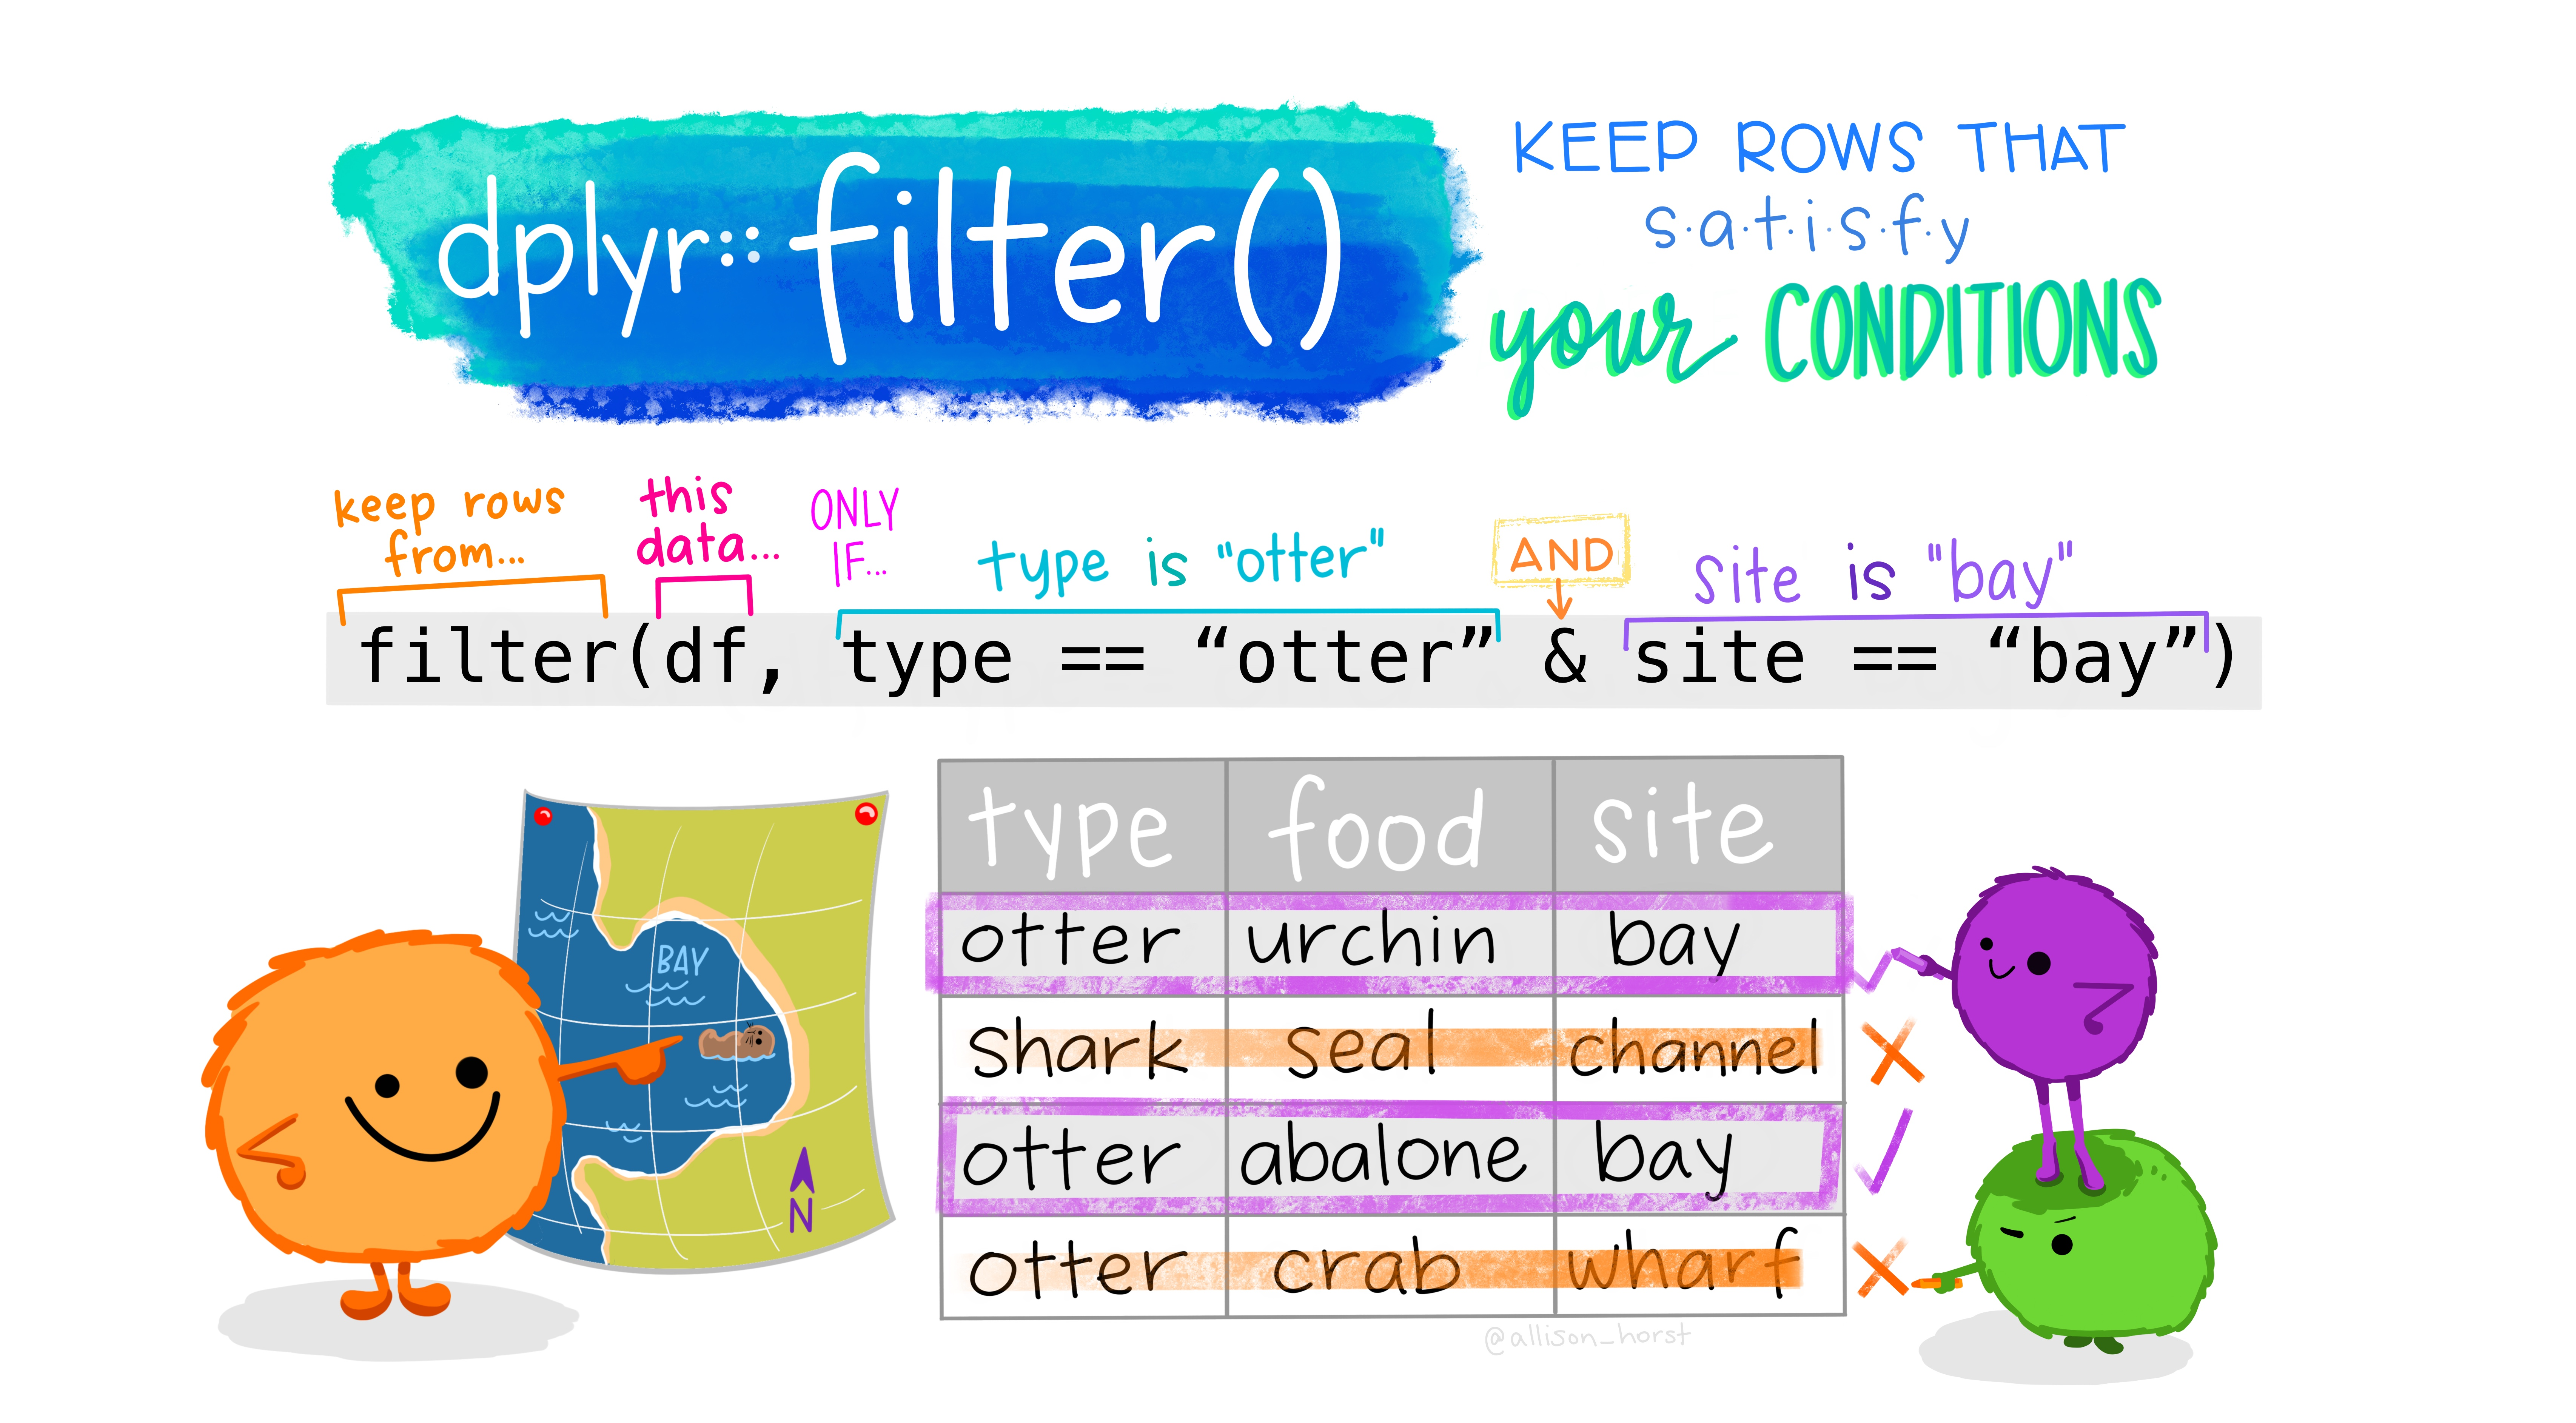
\includegraphics[width=0.8\textwidth,height=\textheight]{Images/dplyr_filter.jpg}
\caption{\textbf{Figure 2.11} Filter by Allison Horst}
\end{figure}

Use the \texttt{filter()} function to subset observations (i.e., rows) based on conditions. For example, we only want those for which the \texttt{injured} variable was equal to 1, so we run:

\begin{Shaded}
\begin{Highlighting}[]
\NormalTok{only\_injured }\OtherTok{\textless{}{-}}\NormalTok{ ncvs }\SpecialCharTok{\%\textgreater{}\%} \FunctionTok{filter}\NormalTok{(injured }\SpecialCharTok{==} \DecValTok{1}\NormalTok{)}
\end{Highlighting}
\end{Shaded}

These filters can be combined using conditions and (\texttt{\&}) and or (\texttt{\textbar{}}) except we call this subset of the data frame `knew\_of\_and\_injured':

\begin{Shaded}
\begin{Highlighting}[]
\CommentTok{\# We want a subset called \textquotesingle{}knew\_of\_and\_injured\textquotesingle{} which comprises responses greater than 0 in the \textquotesingle{}relationship\textquotesingle{} variable and responses equal to 1 in the \textquotesingle{}injured\textquotesingle{} variable}
\NormalTok{knew\_of\_and\_injured }\OtherTok{\textless{}{-}}\NormalTok{ ncvs }\SpecialCharTok{\%\textgreater{}\%} 
\FunctionTok{filter}\NormalTok{(relationship }\SpecialCharTok{\textgreater{}} \DecValTok{0} \SpecialCharTok{\&}\NormalTok{ injured }\SpecialCharTok{==} \DecValTok{1}\NormalTok{)}
\end{Highlighting}
\end{Shaded}

Say if we wanted the first five rows of \texttt{knew\_of\_and\_injured}. How would we do that? In your group googledoc, type out the code you think will help you create a (sub-)subset \texttt{knew\_of\_and\_injured} of its first five rows. Call this new subset `injuredfiveknew'.

\begin{center}\rule{0.5\linewidth}{0.5pt}\end{center}

\hypertarget{activity-9-subsetting-the-sequel}{%
\subsubsection{Activity 9: Subsetting, the Sequel}\label{activity-9-subsetting-the-sequel}}

We now have a subset called \texttt{injuredfiveknew}. Say we only want to keep the variables \texttt{V3014} (age) and \texttt{V3018} (sex). How would you make an object that only contains these two variables from \texttt{injuredfiveknew}?

Recall that you would need to use the function \texttt{select()}to select variables. But in this example, instead of inserting ' : ' like in the previous code, you would need to insert a `,'. Understanding what `:' means and viewing the order of the variables in \texttt{injuredfiveknew} will give you insight into why.

In your group googledoc sheet, write out the code that you would use to do so. Name this new object that contains the two variables \texttt{five\_ageandincome}

\begin{center}\rule{0.5\linewidth}{0.5pt}\end{center}

\hypertarget{summary-1}{%
\section{SUMMARY}\label{summary-1}}

Today you were further introduced to \textbf{tidyverse} packages that helped you to tidy your data. First, we learned to put our work into a \textbf{project} and then how to import data using a package called \texttt{haven}. Whenever we specify a data frame, we learned a nifty short-cut: the \textbf{pipe operator} - \texttt{\%\textgreater{}\%} - which allows us to specify the data frame only once when we code.

Our three main topics today had to do with helping us tidy. There was a lot of \textbf{data wrangling} too. One topic were the variables themselves where we learned about the \textbf{factor} and \textbf{numeric} classes, and how to make and \textbf{recode} new variables. Two, we learned how to remove and add variable and value labels so that we can understand what our variables are measuring. Three, we then learned to subset our data, whereby we make new dataframes that include only the columns -- variables -- or rows -- observations -- we want. We tidied our data using the TIDYVERSE WAY!

P.S. Well done today, to get through all this. What you are learning now will serve as the building blocks for your later data analysis, and we recognise it is all new and scary. But keep practicing, and you will get the hang of this in no time! And of course: don't forget to do your homework!

\hypertarget{answers-to-activities-if-applicable}{%
\subsection{Answers to activities (if applicable)}\label{answers-to-activities-if-applicable}}

\begin{itemize}
\item
  \begin{enumerate}
  \def\labelenumi{\arabic{enumi}.}
  \tightlist
  \item
    N/A
  \end{enumerate}
\item
  \begin{enumerate}
  \def\labelenumi{\arabic{enumi}.}
  \setcounter{enumi}{1}
  \tightlist
  \item
    23,969 entries and 47 columns
  \end{enumerate}
\item
  \begin{enumerate}
  \def\labelenumi{\arabic{enumi}.}
  \setcounter{enumi}{2}
  \tightlist
  \item
    numeric (but is this correct?)- class(ncvs\$weaponpresent)
  \end{enumerate}
\item
  \begin{enumerate}
  \def\labelenumi{\arabic{enumi}.}
  \setcounter{enumi}{3}
  \tightlist
  \item
    N/A
  \end{enumerate}
\item
  \begin{enumerate}
  \def\labelenumi{\arabic{enumi}.}
  \setcounter{enumi}{4}
  \tightlist
  \item
    N/A
  \end{enumerate}
\item
  \begin{enumerate}
  \def\labelenumi{\arabic{enumi}.}
  \setcounter{enumi}{5}
  \tightlist
  \item
    N/A
  \end{enumerate}
\item
  \begin{enumerate}
  \def\labelenumi{\arabic{enumi}.}
  \setcounter{enumi}{6}
  \tightlist
  \item
    N/A
  \end{enumerate}
\item
  \begin{enumerate}
  \def\labelenumi{\arabic{enumi}.}
  \setcounter{enumi}{7}
  \tightlist
  \item
    injuredfiveknew \textless- KnewOfandInjured \%\textgreater\% slice(1:5)
  \end{enumerate}
\item
  \begin{enumerate}
  \def\labelenumi{\arabic{enumi}.}
  \setcounter{enumi}{8}
  \tightlist
  \item
    five\_ageandincome \textless- injuredfiveknew \%\textgreater\% select(4,6)
  \end{enumerate}
\end{itemize}

\hypertarget{data-visualization}{%
\chapter{Data Visualization}\label{data-visualization}}

\hypertarget{layers-and-graphs}{%
\subsubsection*{\texorpdfstring{\emph{Layers and Graphs}}{Layers and Graphs}}\label{layers-and-graphs}}
\addcontentsline{toc}{subsubsection}{\emph{Layers and Graphs}}

\hypertarget{learning-outcomes-2}{%
\paragraph*{\texorpdfstring{\textbf{Learning Outcomes:}}{Learning Outcomes:}}\label{learning-outcomes-2}}
\addcontentsline{toc}{paragraph}{\textbf{Learning Outcomes:}}

\begin{itemize}
\tightlist
\item
  Understand what the layered approach to Grammar of Graphics and its corresponding package \texttt{ggplot2} are
\item
  Learn how to use \texttt{ggplot2} to create different visualizations
\end{itemize}

\hypertarget{todays-learning-tools-2}{%
\paragraph*{\texorpdfstring{\textbf{Today's Learning Tools:}}{Today's Learning Tools:}}\label{todays-learning-tools-2}}
\addcontentsline{toc}{paragraph}{\textbf{Today's Learning Tools:}}

\hypertarget{total-number-of-activities-12}{%
\paragraph*{\texorpdfstring{\emph{Total number of activities}: 12}{Total number of activities: 12}}\label{total-number-of-activities-12}}
\addcontentsline{toc}{paragraph}{\emph{Total number of activities}: 12}

\hypertarget{data-2}{%
\paragraph*{\texorpdfstring{\emph{Data:}}{Data:}}\label{data-2}}
\addcontentsline{toc}{paragraph}{\emph{Data:}}

\begin{itemize}
\tightlist
\item
  Official crime data from England and Wales
\end{itemize}

\hypertarget{packages-3}{%
\paragraph*{\texorpdfstring{\emph{Packages:}}{Packages:}}\label{packages-3}}
\addcontentsline{toc}{paragraph}{\emph{Packages:}}

\begin{itemize}
\tightlist
\item
  \texttt{ggplot2}
\item
  \texttt{ggthemes}
\item
  \texttt{readr}
\item
  \texttt{here}
\end{itemize}

\hypertarget{functions-introduced-and-packages-to-which-they-belong-2}{%
\paragraph*{\texorpdfstring{\emph{Functions introduced (and packages to which they belong)}}{Functions introduced (and packages to which they belong)}}\label{functions-introduced-and-packages-to-which-they-belong-2}}
\addcontentsline{toc}{paragraph}{\emph{Functions introduced (and packages to which they belong)}}

\begin{itemize}
\tightlist
\item
  \texttt{aes()} : Mapping aesthetics to variables (\texttt{ggplot2})
\item
  \texttt{as.factor()} : Convert to factor, including specifying levels (\texttt{base\ R})
\item
  \texttt{facet\_wrap()} : Facet graphics by one or more variables (\texttt{ggplot2})
\item
  \texttt{geom\_histogram()} : Geometry layer for histograms (\texttt{ggplot2})
\item
  \texttt{geom\_line()} : Geometry layer for line charts (\texttt{ggplot2})
\item
  \texttt{geom\_point()} : Geometry layer for scatterplots (\texttt{ggplot2})
\item
  \texttt{ggplot()} : Initialize a ggplot graphic, i.e., specify data, aesthetics (\texttt{ggplot2})
\item
  \texttt{labs()} : Specify labels for ggplot object, e.g., title, caption (\texttt{ggplot2})
\item
  \texttt{range()} : Compute the minimum and maximum values (\texttt{base\ R})
\item
  \texttt{read\_csv()} : Read in comma separated values file (\texttt{readr})
\item
  \texttt{scale\_color\_brewer()} : Default color scheme options (\texttt{ggplot2})
\item
  \texttt{scale\_color\_viridis\_d()} : Colour-blind-considerate palettes from \texttt{viridis} package (\texttt{ggplot2})
\item
  \texttt{theme()} : Customise ggplot graphics (\texttt{ggplot2})
\item
  \texttt{theme\_economist\ ()} : Changes the graphic to resemble ones found in \emph{The Economist} (\texttt{ggthemes})
\item
  \texttt{theme\_minimal()} : Default minimalist theme for \texttt{ggplot} graphics (\texttt{ggplot2})
\end{itemize}

\begin{center}\rule{0.5\linewidth}{0.5pt}\end{center}

\hypertarget{grammar-of-graphics}{%
\section{Grammar of Graphics}\label{grammar-of-graphics}}

Today we learn the basics of data visualization in \texttt{R} using a package called \texttt{ggplot2} within the \texttt{tidyverse}, one of the most popular packages for making high-quality, reproducible graphics. The framework on which \texttt{ggplot2} is based derives from \href{http://vita.had.co.nz/papers/layered-grammar.pdf}{Hadley Wickham's (2010) A Layered Grammar of Graphics}.

Wickham advances the work of \emph{Grammar of Graphics} by proposing a layered approach to describe and build graphics in a structured manner. Layers, according to Wickham, are used to describe the basic features that underlie any graphic or visualization. Every layer comprises five parts: data, aesthetics, statistical transformation (stat), geometric object (geom), and position adjustment (position).

The three primary ones we focus on to ease you into this, however, are (1) the data, (2) the aesthetics, and (3) the geometric objects:

\begin{enumerate}
\def\labelenumi{\arabic{enumi}.}
\item
  Data: usually the data frame with tidy rows and columns.
\item
  Aesthetics: the visual characteristics that represent the data, or variables. At its simplest, these could be an x- and y-axis, and can extend to other aesthetics like colour, size, and shape, which are mapped to variables.
\item
  Geometric objects: also known as `geoms' and represent the data points in the visualization, such as dots or lines.
\end{enumerate}

\begin{figure}
\centering
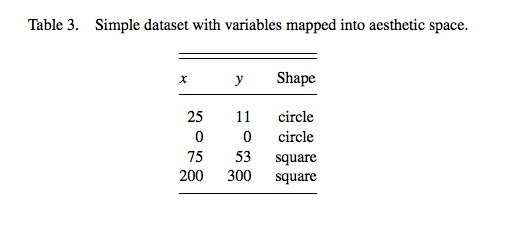
\includegraphics[width=0.7\textwidth,height=\textheight]{Images/grammar1.png}
\caption{\textbf{Figure 3.1} Visualize Table 3}
\end{figure}

\begin{figure}
\centering
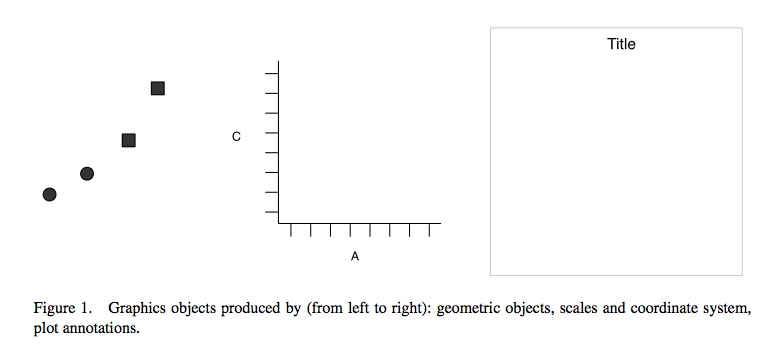
\includegraphics[width=0.7\textwidth,height=\textheight]{Images/grammar 2.png}
\caption{\textbf{Figure 3.2} Using the \emph{Grammar of Graphics} approach to convert elements of Table 3 into its visual components}
\end{figure}

\begin{figure}
\centering
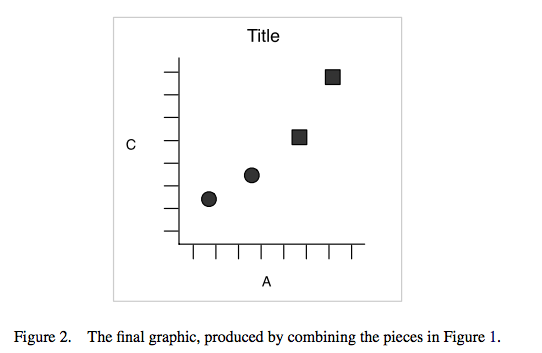
\includegraphics[width=0.7\textwidth,height=\textheight]{Images/grammar3.png}
\caption{\textbf{Figure 3.3} Integrating those visual parts of Table 3 into a graphic}
\end{figure}

Why is this important? Visualizing your data helps you to have a better understanding of them before moving on to more advanced and complex analyses. Numbers themselves can be deceptive and complicated, so by visualizing them, you can identify any patterns or anomalies.

\hypertarget{activity-1-getting-ready}{%
\subsection{Activity 1: Getting Ready}\label{activity-1-getting-ready}}

Before we `layer up', let us do the following:

\begin{enumerate}
\def\labelenumi{\arabic{enumi}.}
\item
  Open up your existing \texttt{R}project like you had learned last week
\item
  Load the \texttt{ggplot2} and \texttt{readr} packages using the \texttt{library()} function. If you have not already installed these packages, you will need to do so first, using the \texttt{install.packages()} function. \emph{If you are unclear about the difference between these two functions, see 1.3.3 in Lesson 1 of this online tutorial site or ask now!}
\item
  Download the first two datasets (gmp\_2017.csv and gmp\_monthly\_2017.csv) from Blackboard, in the subfolder `Data for this week' in the Week 3 learning materials. The datasets contain crime data from Greater Manchester, England. Load these two datasets using the \texttt{read\_csv()} function into two separate data frames. Respectively name the data frames \texttt{burglary\_df} and \texttt{monthly\_df} by using the \texttt{\textless{}-} assignment operator.
\end{enumerate}

Make sure the datasets are saved in the sub-folder called `Datasets' that you created last week \emph{inside} your project directory/ folder. If this is the case, we can use the \texttt{here()} function to tell \texttt{R} where exactly to locate the datasets. (See lecture short 3.1 `The R Prep routine' on Blackboard.)

Create first data frame object, \texttt{burglary\_df} and load into it the `gmp\_2017.csv' data file:

\begin{Shaded}
\begin{Highlighting}[]
\CommentTok{\# gmp\_2017.csv}
\NormalTok{burglary\_df }\OtherTok{\textless{}{-}} \FunctionTok{read\_csv}\NormalTok{(}\FunctionTok{here}\NormalTok{(}\StringTok{"Datasets"}\NormalTok{, }\StringTok{"gmp\_2017.csv"}\NormalTok{))}
\end{Highlighting}
\end{Shaded}

Now your turn to make the second data frame. Create the second data frame, \texttt{monthly\_df} and load into it the `gmp\_monthly\_2017.csv' data file.

You should have two data frames in your environment now. How many observations (rows) and variables (columns) are in \texttt{burglary\_df}? How about in \texttt{monthly\_df}?

\begin{center}\rule{0.5\linewidth}{0.5pt}\end{center}

\hypertarget{ggplot2}{%
\section{ggplot2}\label{ggplot2}}

This week we will be learning how to use \texttt{R} to create various exciting data visualizations. You may remember some of the key principles of data visualizations from last semester: graphics should be truthful,functional, beautiful, insightful, and enlightening. Also, accessible!

Here is a recent powerful visualization from The New York Times about deaths from COVID-19 in the USA (Figure 3.4): \url{https://twitter.com/beccapfoley/status/1363338950518206472}

\begin{figure}
\centering
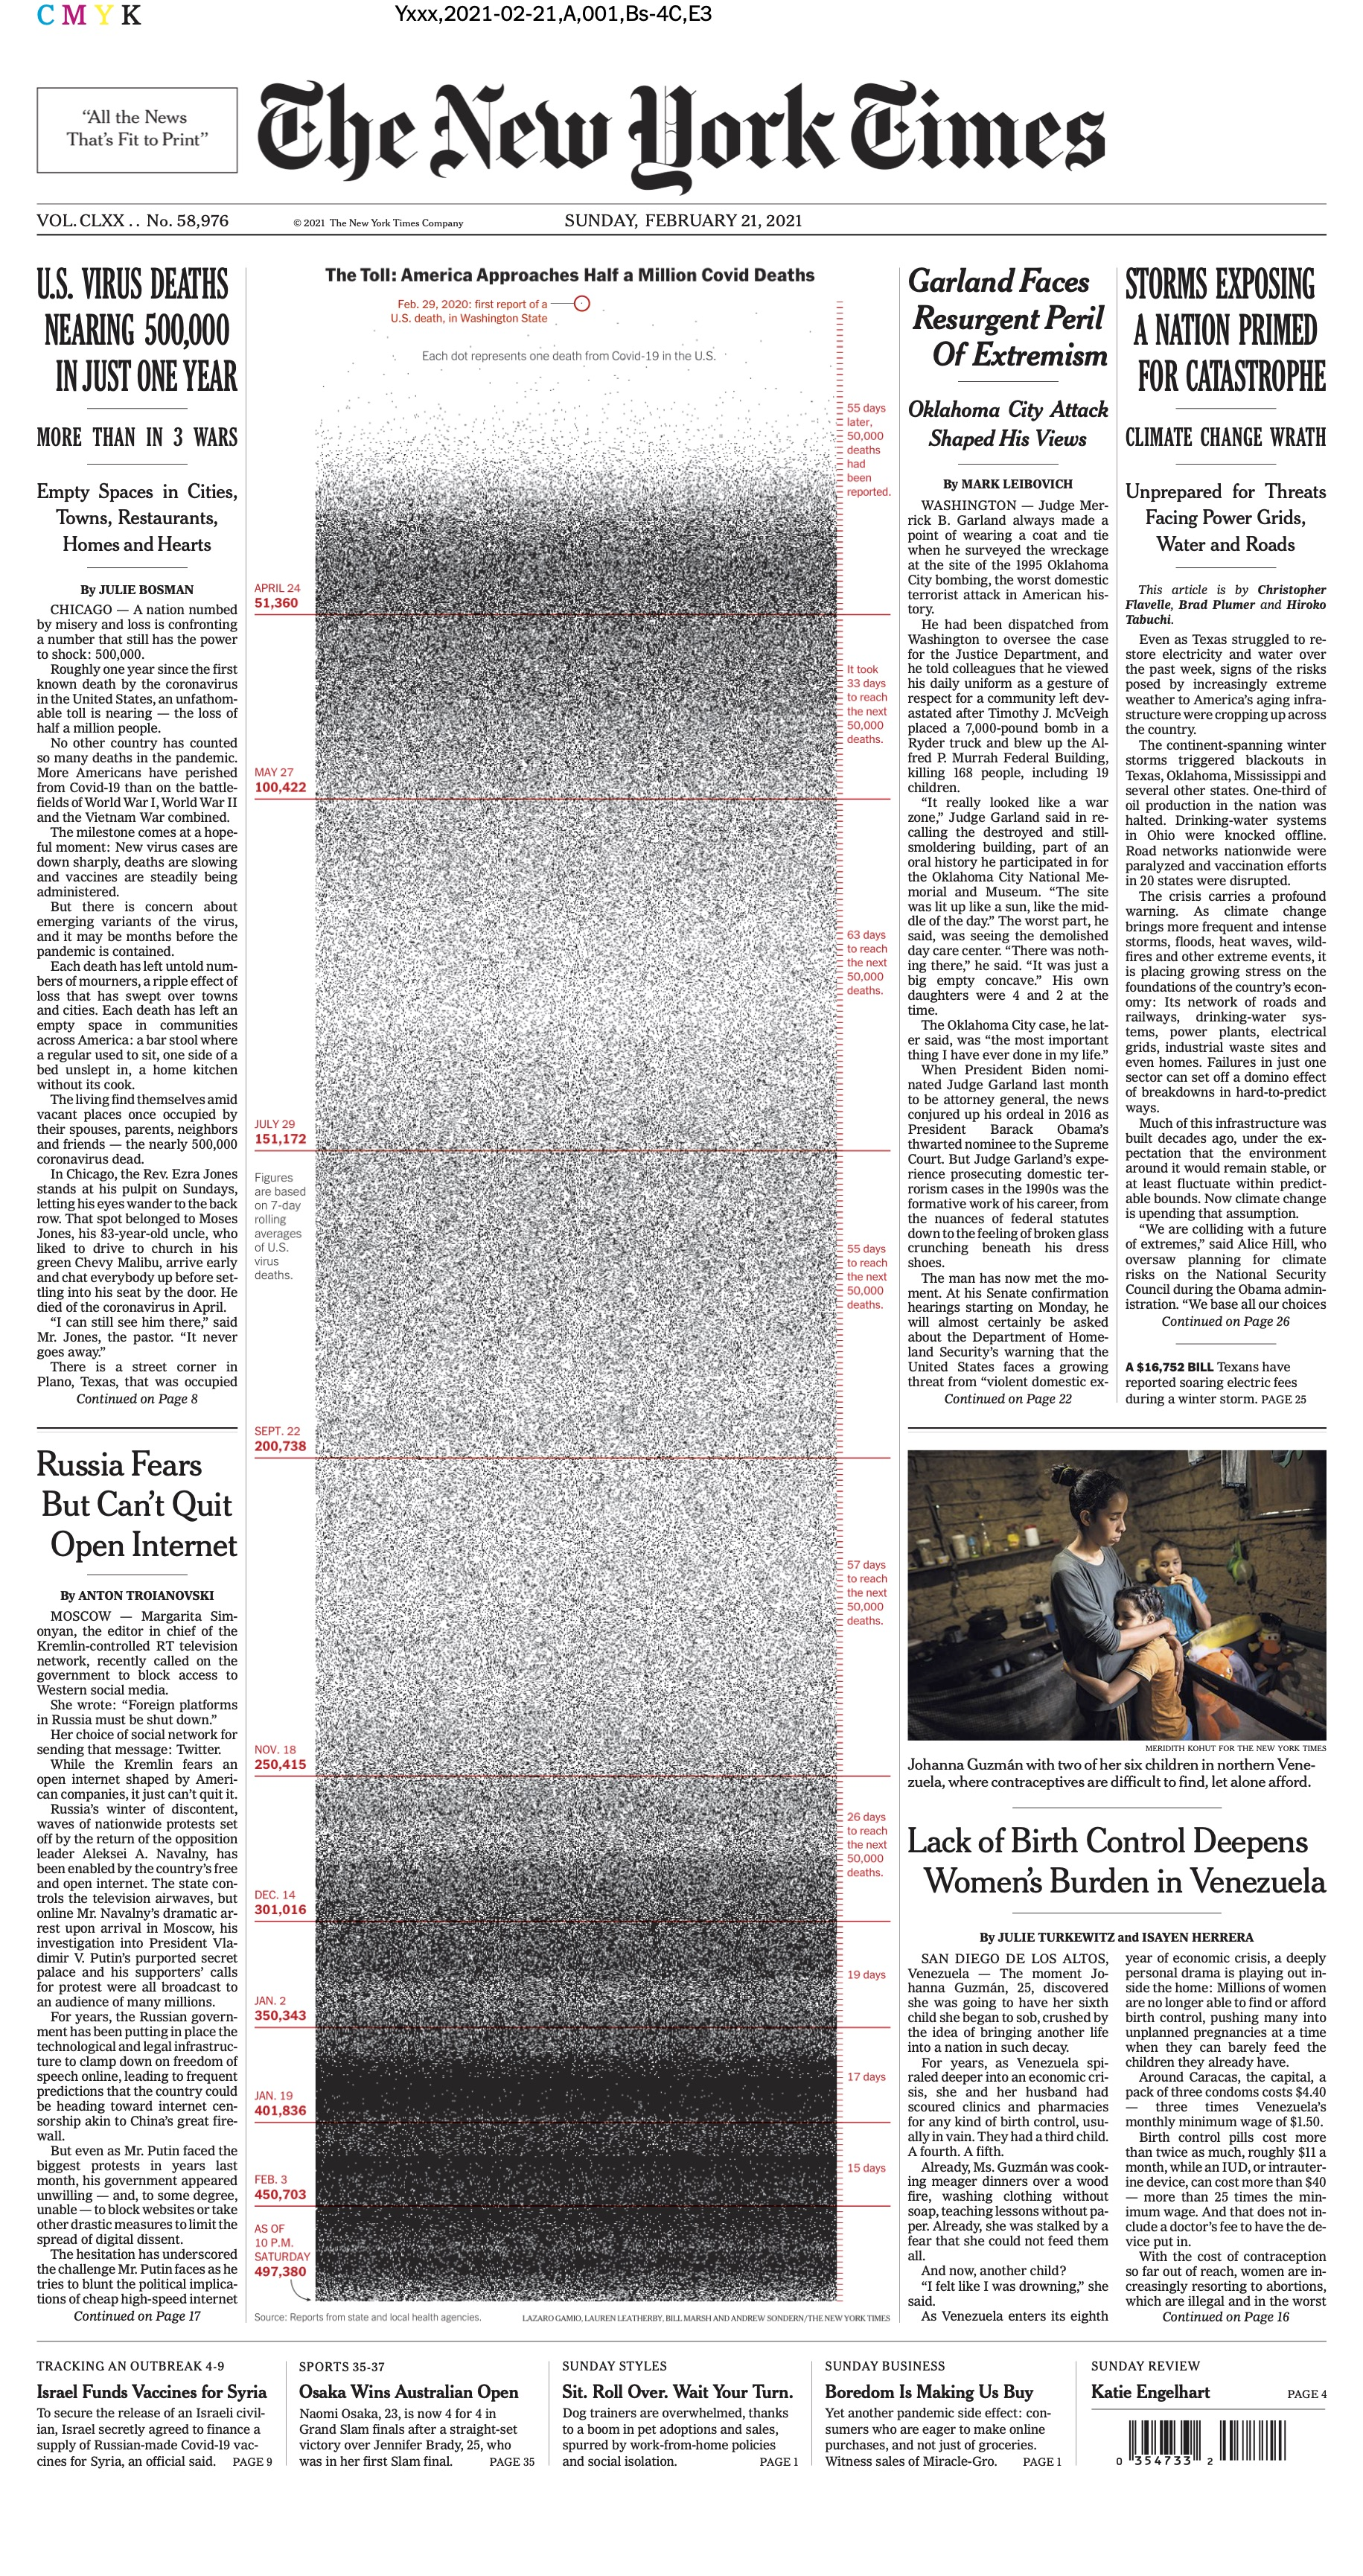
\includegraphics[width=0.7\textwidth,height=\textheight]{Images/times_COVID_VIZ.jpeg}
\caption{\textbf{Figure 3.4} NYT visualization of COVID-19 deaths in USA}
\end{figure}

\texttt{R} has amazing data visualization qualities. It is increasingly used by professionals and academics to create graphics that embody those principles of data visualization.

For example, read this article about how the BBC uses \texttt{R} to create their graphics: \href{https://medium.com/bbc-visual-and-data-journalism/how-the-bbc-visual-and-data-journalism-team-works-with-graphics-in-r-ed0b35693535}{How the BBC Visual and Data Journalism team works with graphics in R} (See Figure 3.5)

\begin{figure}
\centering
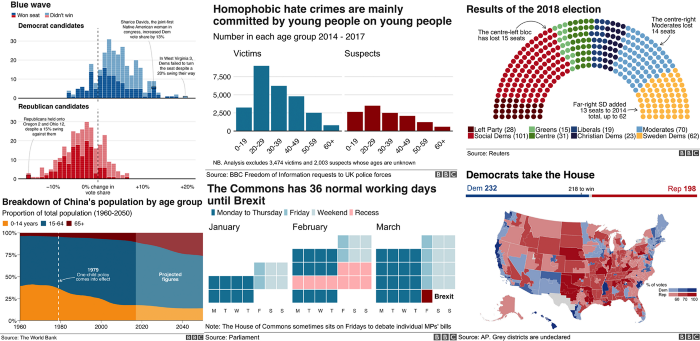
\includegraphics{Images/bbc_r.png}
\caption{\textbf{Figure 3.5} How the BBC Visual and Data Journalism team works with graphics in R}
\end{figure}

As you learn to create graphs in \texttt{ggplot2}, you will see that the code reflects building these graphs as layers. This will take getting used to if you are only familiar with building graphs from a template in Excel. You can also reuse chunks of code to create different kinds of graphics or identical ones in other datasets.

Today we focus on the \texttt{ggplot2} package to learn our three substantive topics: \textbf{layers}, \textbf{graphs for categorical data}, and \textbf{graphs for numeric data}.

\hypertarget{activity-2-getting-to-know-new-data}{%
\subsubsection{Activity 2: Getting to Know New Data}\label{activity-2-getting-to-know-new-data}}

Before we dive into those topics, we need to get into the habit of getting to know our data. Below is a brief `data dictionary' of the variables from both of our data:

A. \textbf{burglary\_df} has nine variables:

\begin{itemize}
\tightlist
\item
  \emph{LSOAcode}: LSOA stands for Lower Super Output Area, and is a statistical unit of geography. It represents neighbourhoods that each contain 300-400 households. Essentially, LSOA means neighbourhood.
\item
  \emph{burglary\_count}: the number of burglaries in each LSOA in 2017
\item
  \emph{LAname}: the name of the Local Authority into which the LSOA falls
\item
  \emph{IMD score}: the IMD refers to the Index of Multiple Deprivation. This measure combines seven domains of deprivation into one index: (1) income, (2) employment, (3) education, (4) health, (5) crime, (6) barriers to housing or services, and (7) living environment. It is the score that a particular LSOA has on this measure. You can read more about the measure here: \href{https://assets.publishing.service.gov.uk/government/uploads/system/uploads/attachment_data/file/833959/IoD2019_Infographic.pdf}{IMD infographic}\\
\item
  \emph{IMDrank}: another version of the IMD except it ranks all 32,844 LSOAs from highest to lowest deprivation.
\item
  \emph{IMDdeci}: indicates in what decile of deprivation the LSOA falls.
\item
  \emph{incscore}: score for income deprivation; this is one of the seven indicators comprising the IMD. Measures the proportion of the population experiencing deprivation relating to low income.
\item
  \emph{LSOAname}: the name of that particular LSOAs
\item
  \emph{pop}: the population size of LSOAs
\end{itemize}

B. \textbf{monthly\_df} has three variables:

\begin{itemize}
\tightlist
\item
  \emph{Month}: month of the year whereby 1 = January, 2 = February\ldots{} and 12 = December
\item
  \emph{crime\_type}: type of crime (for police.uk categories, see: \href{https://www.police.uk/SysSiteAssets/police-uk/media/downloads/crime-categories/police-uk-category-mappings.csv}{download police.uk data categories vs home office offence codes})
\item
  \emph{n}: number of each type of crime for each month in 2017
\end{itemize}

Have a look at both datasets. Let us use the function \texttt{View()} first. What do you think are the levels of measurement for each variable? Make a note of this.

Now use the the function \texttt{class()} to look at how \texttt{R} treats each variable for each dataset. How does this match with what you think is the level of measurement for each variable? Keep this in mind!

Notice that although \texttt{monthly\_df} has only several variables, there is a lot of information in this data frame. There are counts for various different crimes for each month of the year. Because of this, the data are in \emph{long format}. This is a useful and typical format for longitudinal data because our time variable (i.e., months) is contained in one variable. This will make it easier to create graphics showing change over time.

In addition, when you read a good quantitative research paper, its methods section will state the number of cases analysed with `n =', whereby `n' represents `number of cases'. This is known as sample size. For example, if the sample size of a study is two-hundred, the methods section would state it as `n= 200'.

In your group google doc, type out the following: the number of observations for each data frame. Type out these values following `n ='. In addition, state what you think the unit of analysis is in each data frame.

\begin{center}\rule{0.5\linewidth}{0.5pt}\end{center}

\hypertarget{todays-3}{%
\section{Today's 3}\label{todays-3}}

Now that we have gotten to know our data, onto our three main topics: \textbf{layers}, \textbf{graphs for nominal and ordinal data}, and \textbf{graphs for interval and ratio data}.

\begin{center}\rule{0.5\linewidth}{0.5pt}\end{center}

\hypertarget{layers}{%
\subsection{Layers}\label{layers}}

Layers often relate to one another and have similar features. For example, they may share the same underlying data on which they are built. An example is this scatterplot overlayed with a smoothed regression line to describe the relationship between two variables:

\begin{figure}
\centering
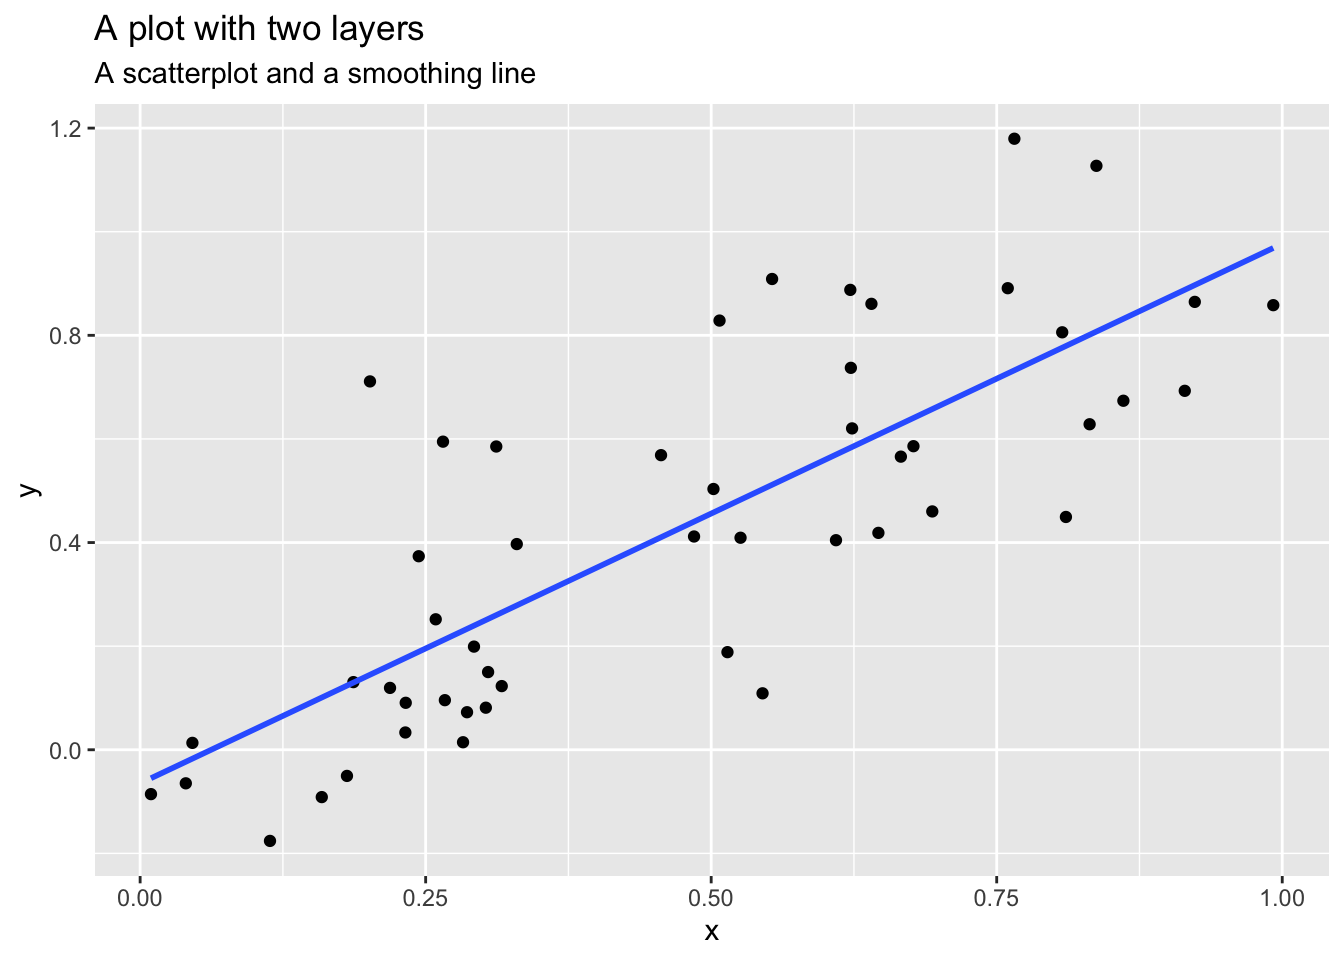
\includegraphics[width=0.7\textwidth,height=\textheight]{Images/layers.png}
\caption{\textbf{Figure 3.6} A graphic with two layers}
\end{figure}

From: \url{https://cfss.uchicago.edu/notes/grammar-of-graphics/}

One layer is the scatterplot itself and it contains the necessary components (e.g., data, aesthetics, and geom). The second layer is the smoothing line. Another example of multiple layers is this one that uses two different but related datasets in one graphic:

\begin{figure}
\centering
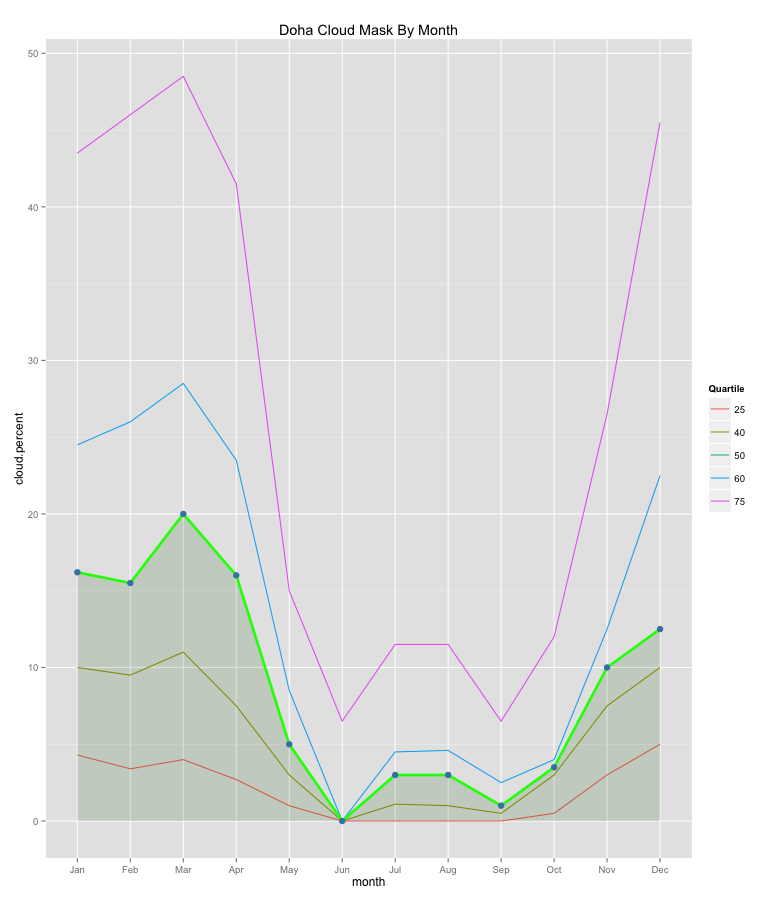
\includegraphics[width=0.7\textwidth,height=\textheight]{Images/complexlayer.png}
\caption{\textbf{Figure 3.7} Different data sets and aesthetics defined by layer}
\end{figure}

From: \url{http://applied-r.com/building-layered-plots/}

The advantage of the layered approach is its ease for the user and the developer of these statistical graphics. As a user, you can repeatedly update a graphic, changing one feature at a time instead of having to work with the overall graphic; as a developer, you can add more components to your graphic while being able to use what you have already. The idea is that you can tweak your graphic by component or layer while leaving the rest of your graphic intact. This is in constrast to changing the entire graphic just to tweak a small detail.

To understand a layer and how it is generated in \texttt{ggplot2}, we begin with a scatterplot. This is a graph that shows the relationship between two continuous variables -- in other words, between two numeric variables.

For example, we may be interested to find out whether there is a relationship between area-level income deprivation and burglaries. Are areas with higher income deprivation scores burgled more? Perhaps there is less money to spend on security systems, so there is easier access to homes in these areas. Or is it areas with lower income deprivation scores that are burgled more? Maybe because these areas are wealthier so there are more valuable goods to take. To visualize this relationship, we build a scatterplot using the layered approach.

\hypertarget{activity-3-using-ggplot2-to-create-a-scatterplot}{%
\subsubsection{Activity 3: Using ggplot2 to create a scatterplot}\label{activity-3-using-ggplot2-to-create-a-scatterplot}}

Our research question, therefore, is: \emph{What is the relationship between income and burglary counts?}

Following the grammar of graphics layered approach, let us first specify the data component. To do this, we take the \texttt{ggplot()} function, and inside it, we put our data frame object, which contains our data. To let the function know this is the data, we can also write \texttt{data\ =} before it:

\begin{Shaded}
\begin{Highlighting}[]
\CommentTok{\# If there is an error about function missing, has the package ggplot2 been installed and loaded?}

\FunctionTok{ggplot}\NormalTok{(}\AttributeTok{data =}\NormalTok{ burglary\_df)}
\end{Highlighting}
\end{Shaded}


\includegraphics{03-data-visualisation_files/figure-latex/unnamed-chunk-4-1.pdf}

The \emph{Plots} window will appear and will be blank, like what you see above. We have told \texttt{R} what data we want to plot, but we have yet to specify what variables we want across our x and y axes, or other fields. To do this, we will need \emph{aesthetics}, the second component of the layer.

Recall that aesthetics are about mapping the visual properties. As our research question is about the relationship between income (\texttt{incscore}) and burglary count (\texttt{burglary\_count}), we will map these variables to the x and y axes. We specify the aesthetics inside the \texttt{aes()} function (i.e.,\textbf{aes}thetics), indicating which variable we want on the x axis (\texttt{x\ =}) and which one on the y axis (\texttt{y\ =}).

\begin{Shaded}
\begin{Highlighting}[]
\FunctionTok{ggplot}\NormalTok{(}\AttributeTok{data =}\NormalTok{ burglary\_df, }\AttributeTok{mapping =} \FunctionTok{aes}\NormalTok{(}\AttributeTok{x =}\NormalTok{ incscore, }\AttributeTok{y =}\NormalTok{ burglary\_count))}
\end{Highlighting}
\end{Shaded}

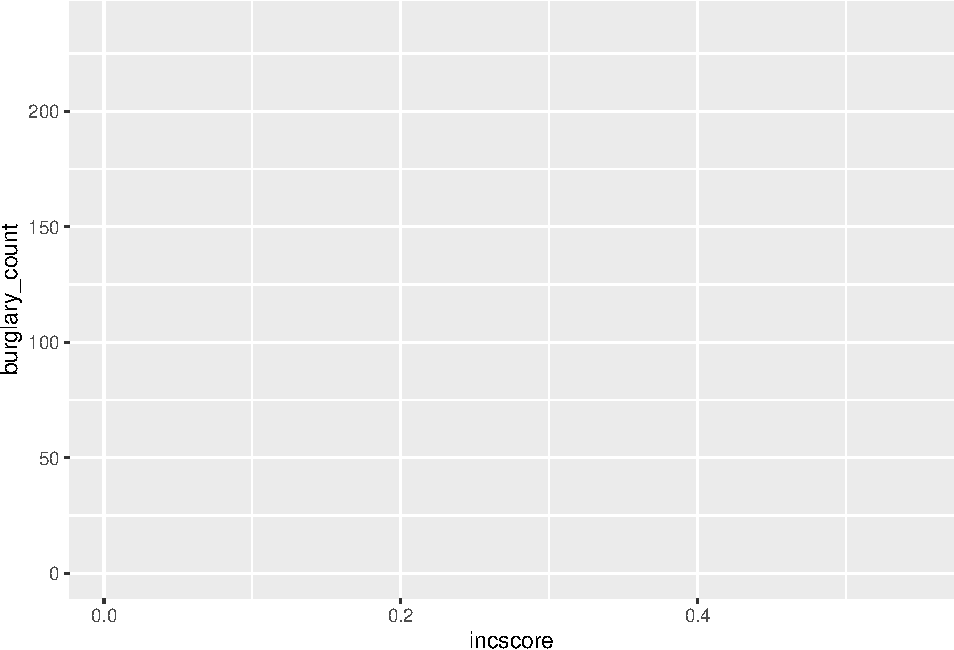
\includegraphics{03-data-visualisation_files/figure-latex/unnamed-chunk-5-1.pdf}

You will now see an update in the \emph{Plots} window! It shows the axis and the axes labels. \texttt{R} now knows that we want to plot the income variable on our x axis and the burglary count variable on the y. The labels are applied automatically, but you can change these, which we will soon learn.

Let us learn how to finally put our data on the plot. To do this, we must assign a \textbf{geometry}.

This last component is the geometric object, and is what also makes the layer in \texttt{R} code. It has numerous functions, each beginning with the argument \texttt{geom\_}. To create a scatterplot, we use the function \texttt{geom\_point()}:

\begin{Shaded}
\begin{Highlighting}[]
\FunctionTok{ggplot}\NormalTok{(}\AttributeTok{data =}\NormalTok{ burglary\_df, }\AttributeTok{mapping =} \FunctionTok{aes}\NormalTok{(}\AttributeTok{x =}\NormalTok{ incscore, }\AttributeTok{y =}\NormalTok{ burglary\_count)) }\SpecialCharTok{+}
  \FunctionTok{geom\_point}\NormalTok{()}
\end{Highlighting}
\end{Shaded}

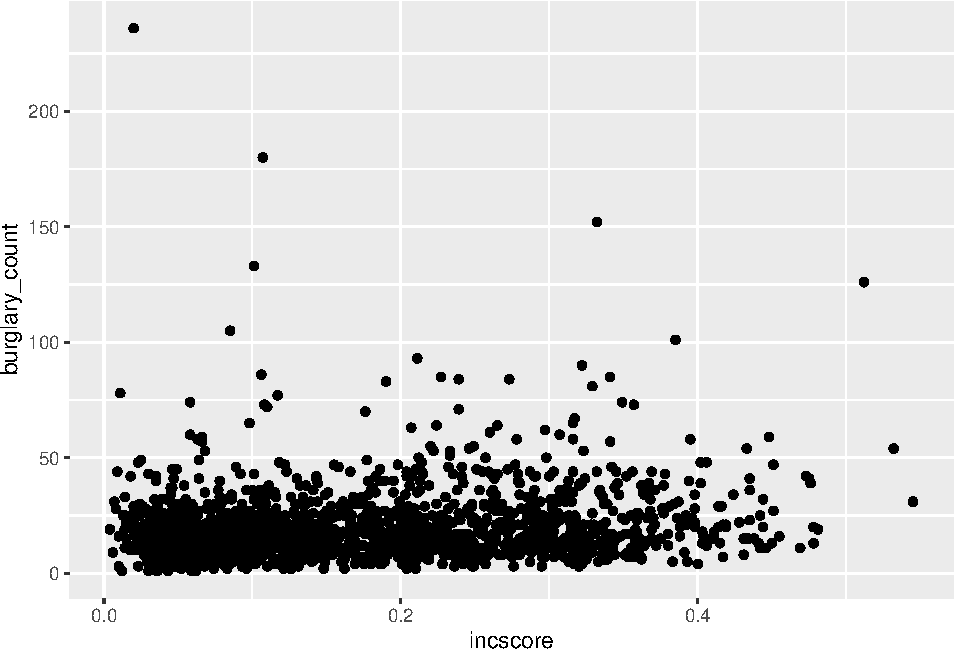
\includegraphics{03-data-visualisation_files/figure-latex/unnamed-chunk-6-1.pdf}

\begin{Shaded}
\begin{Highlighting}[]
\CommentTok{\# We are saying, ‘Hey R, may you please make me a graphic using the data "burglary\_df” and map the variables “incscore” to the x{-}axis and “burglary\_count” to the y{-}axis, then pass this information through (using “ + ” ) to make a scatterplot?’}
\end{Highlighting}
\end{Shaded}

Now the scatterplot in all its glory appears. What can you say about the relationship between deprivation and burglary victimisation? In your group google doc, type out what you think is the relationship between these two variables.

\begin{center}\rule{0.5\linewidth}{0.5pt}\end{center}

\hypertarget{activity-4-adding-a-third-variable-to-a-scatterplot}{%
\subsubsection{Activity 4: Adding a Third Variable to a Scatterplot}\label{activity-4-adding-a-third-variable-to-a-scatterplot}}

The real power in layered graphics comes from the ability to keep piling on the layers and tweaking components that make up the layers. For example, it would be helpful if we included other information like how local authorities may play a role in this relationship. Maybe income is positively associated with burglaries in one local authority, such as Bolton, but not in another, such as Bury. To explore this, we might want to colour each point by the variable \texttt{LAname} using the \texttt{colour} argument:

\begin{Shaded}
\begin{Highlighting}[]
\FunctionTok{ggplot}\NormalTok{(}\AttributeTok{data =}\NormalTok{ burglary\_df, }\AttributeTok{mapping =} \FunctionTok{aes}\NormalTok{(}\AttributeTok{x =}\NormalTok{ incscore, }\AttributeTok{y =}\NormalTok{ burglary\_count, }\AttributeTok{colour =}\NormalTok{ LAname)) }\SpecialCharTok{+} 
  \FunctionTok{geom\_point}\NormalTok{()}
\end{Highlighting}
\end{Shaded}

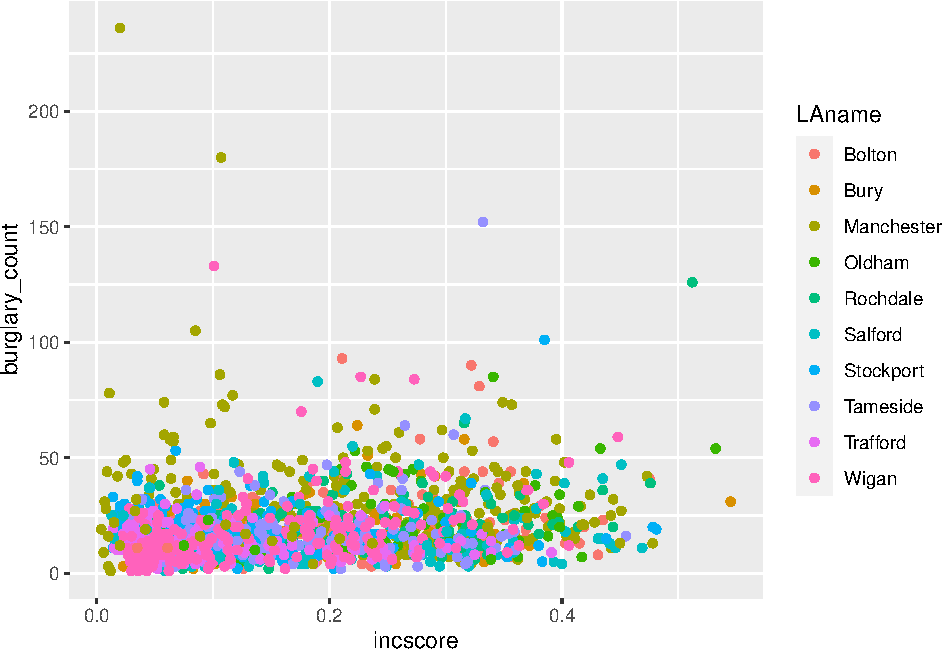
\includegraphics{03-data-visualisation_files/figure-latex/unnamed-chunk-7-1.pdf}

In your group google doc, state what you observe from this new visual. What sort of relationship does it seem to show between burglary counts and income? Do you think local authority plays a role? Do note the default colours, and think back to what we learned about accessibility last semester. In the next activity, we will address this!

\begin{center}\rule{0.5\linewidth}{0.5pt}\end{center}

As previously mentioned, a number of other functions are available for the \texttt{geom\_} function such as shape, linetype, size, fill, and alpha (transparency). But these depend on the geometry being used and the class of variable being mapped to the aesthetic. For example, try the shape aesthetic for \texttt{LAname}, which will vary the shape of each point according to local authority (hint: replace \texttt{colour\ =} with \texttt{shape\ =}). A warning message appears -- what is it telling you? How can you see this reflected on the plot?

This relates to the grammar of graphics philosophy on how people understand information, and \texttt{ggplot2} will warn you when it thinks the graphic is difficult to interpret or, worse, misleading.

\begin{center}\rule{0.5\linewidth}{0.5pt}\end{center}

\hypertarget{activity-5-colours}{%
\subsubsection{Activity 5: Colours!}\label{activity-5-colours}}

The colour palette that appeared for our previous scatterplot is a default one, and there are a number of default colour palettes available. We can specify a colour palette using an additional layer with the function \texttt{scale\_color\_brewer()}. For example:

\begin{Shaded}
\begin{Highlighting}[]
\FunctionTok{ggplot}\NormalTok{(}\AttributeTok{data =}\NormalTok{ burglary\_df, }\AttributeTok{mapping =} \FunctionTok{aes}\NormalTok{(}\AttributeTok{x =}\NormalTok{ incscore, }\AttributeTok{y =}\NormalTok{ burglary\_count, }\AttributeTok{color =}\NormalTok{ LAname)) }\SpecialCharTok{+} 
  \FunctionTok{geom\_point}\NormalTok{() }\SpecialCharTok{+} 
  \FunctionTok{scale\_colour\_brewer}\NormalTok{(}\AttributeTok{palette =} \StringTok{"Spectral"}\NormalTok{)}
\end{Highlighting}
\end{Shaded}

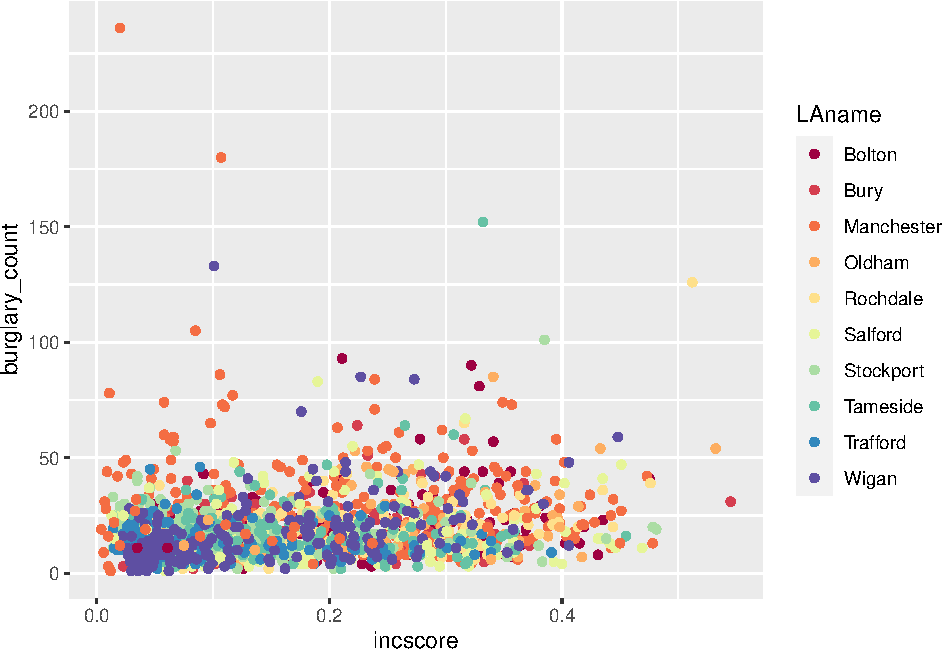
\includegraphics{03-data-visualisation_files/figure-latex/unnamed-chunk-8-1.pdf}

Does that look familiar? Last semester we used the website \href{https://colorbrewer2.org/}{colorbrewer2.org/}. The \texttt{scale\_colour\_brewer()} function takes palettes from this resource, and applies them to your charts.

In addition, the \texttt{viridis} package has a number of colour palettes that consider colour blindness where readers are unable to differentiate colours on the graphic. It is already integrated into \texttt{ggplot2}, so there is no need to install it separately. For example, we take the previous code and replace the last line with a viridis colour palette for categorical variables:

\begin{Shaded}
\begin{Highlighting}[]
\FunctionTok{ggplot}\NormalTok{(}\AttributeTok{data =}\NormalTok{ burglary\_df, }\AttributeTok{mapping =} \FunctionTok{aes}\NormalTok{(}\AttributeTok{x =}\NormalTok{ incscore, }\AttributeTok{y =}\NormalTok{ burglary\_count, }\AttributeTok{color =}\NormalTok{ LAname)) }\SpecialCharTok{+} 
  \FunctionTok{geom\_point}\NormalTok{() }\SpecialCharTok{+} 
  \FunctionTok{scale\_color\_viridis\_d}\NormalTok{() }\CommentTok{\# or scale\_color\_viridis\_c() for a continuous variable }
\end{Highlighting}
\end{Shaded}

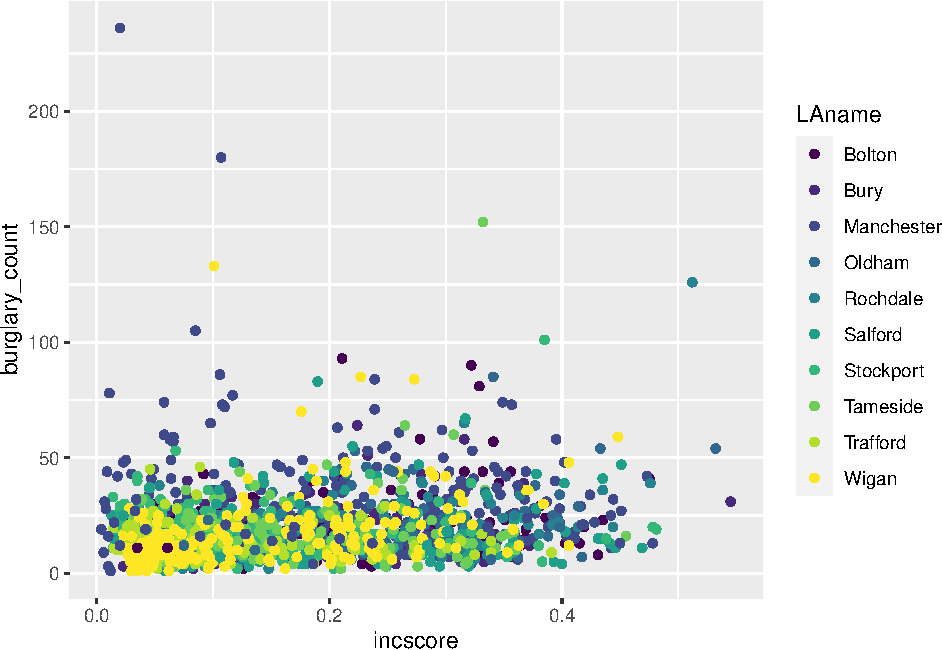
\includegraphics{03-data-visualisation_files/figure-latex/unnamed-chunk-9-1.pdf}

Now we have built up a graph to visualise the bivariate relationship between income deprivation score and burglary count per neighbourhood. Then, we introduced a third variable (i.e., multi-variable analysis) and brought in colour to add to the local authority. In the upcoming exercises, we will learn how to tweak the graphics so to make them even more our own!

\begin{center}\rule{0.5\linewidth}{0.5pt}\end{center}

\hypertarget{activity-6-sizes-transparency}{%
\subsubsection{Activity 6: Sizes \& Transparency}\label{activity-6-sizes-transparency}}

Recall that the geometric object is about the data points themselves. You can change their appearance within the \texttt{geom\_point} function. To increase the size of the points and make them transparent, we use the size and alpha arguments. The default for size is 1, so anything lower than 1 will make points smaller while anything larger than 1 will make the points bigger. The default for alpha is also 1, which means total opaqueness, so you can only go lower to make things more transparent. For example:

\begin{Shaded}
\begin{Highlighting}[]
\CommentTok{\# Below, we want our data points to be a bit bigger ( 3 ) and more transparent ( 0.5 ) than the default}

\FunctionTok{ggplot}\NormalTok{(}\AttributeTok{data =}\NormalTok{ burglary\_df, }\AttributeTok{mapping =} \FunctionTok{aes}\NormalTok{(}\AttributeTok{x =}\NormalTok{ incscore, }\AttributeTok{y =}\NormalTok{ burglary\_count, }\AttributeTok{color =}\NormalTok{ LAname)) }\SpecialCharTok{+} 
  \FunctionTok{geom\_point}\NormalTok{(}\AttributeTok{size =} \DecValTok{3}\NormalTok{, }\AttributeTok{alpha =} \FloatTok{0.5}\NormalTok{) }\SpecialCharTok{+} 
  \FunctionTok{scale\_color\_brewer}\NormalTok{(}\AttributeTok{palette =} \StringTok{"Spectral"}\NormalTok{)}
\end{Highlighting}
\end{Shaded}

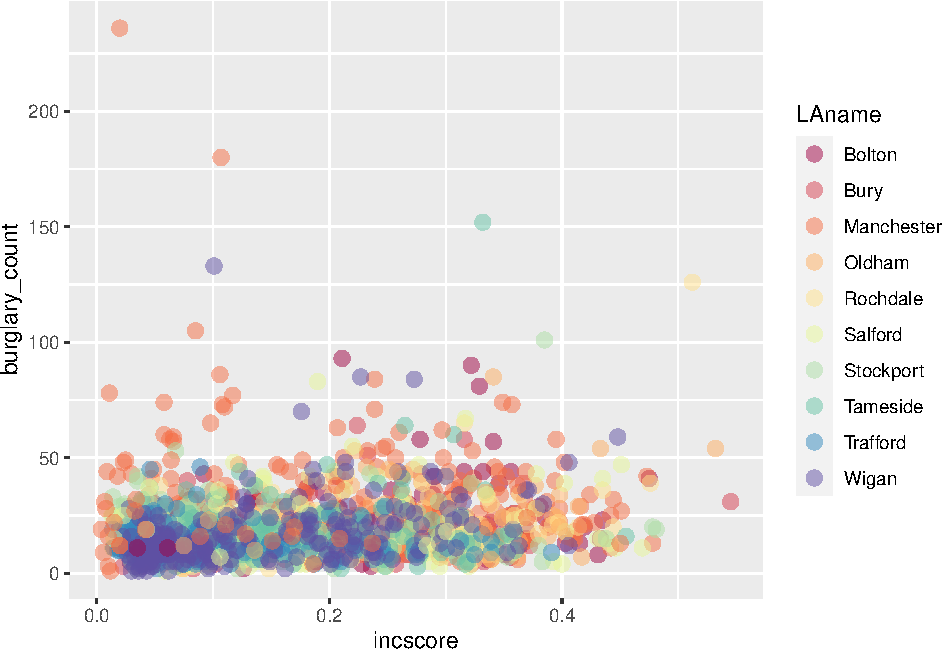
\includegraphics{03-data-visualisation_files/figure-latex/unnamed-chunk-10-1.pdf}

\begin{center}\rule{0.5\linewidth}{0.5pt}\end{center}

\hypertarget{activity-7-labels}{%
\subsubsection{Activity 7: Labels}\label{activity-7-labels}}

The graphic is looking good, but the labels will need tweaking if we do not like the default ones, which are our variable names. We use the \texttt{labs()} function to change the labels for the x and y axes as well as the graphic title:

\begin{Shaded}
\begin{Highlighting}[]
\FunctionTok{ggplot}\NormalTok{(}\AttributeTok{data =}\NormalTok{ burglary\_df, }\AttributeTok{mapping =} \FunctionTok{aes}\NormalTok{(}\AttributeTok{x =}\NormalTok{ incscore, }\AttributeTok{y =}\NormalTok{ burglary\_count, }\AttributeTok{color =}\NormalTok{ LAname)) }\SpecialCharTok{+} 
  \FunctionTok{geom\_point}\NormalTok{(}\AttributeTok{size =} \DecValTok{3}\NormalTok{, }\AttributeTok{alpha =} \FloatTok{0.5}\NormalTok{) }\SpecialCharTok{+} 
  \FunctionTok{scale\_color\_brewer}\NormalTok{(}\AttributeTok{palette =} \StringTok{"Spectral"}\NormalTok{) }\SpecialCharTok{+} 
  \FunctionTok{labs}\NormalTok{(}\AttributeTok{x =} \StringTok{"Income score"}\NormalTok{, }\AttributeTok{y =} \StringTok{"Burglary count"}\NormalTok{, }\AttributeTok{title =} \StringTok{"Income and burglary and victimization"}\NormalTok{, }\AttributeTok{color =} \StringTok{"Local Authority"}\NormalTok{)}
\end{Highlighting}
\end{Shaded}

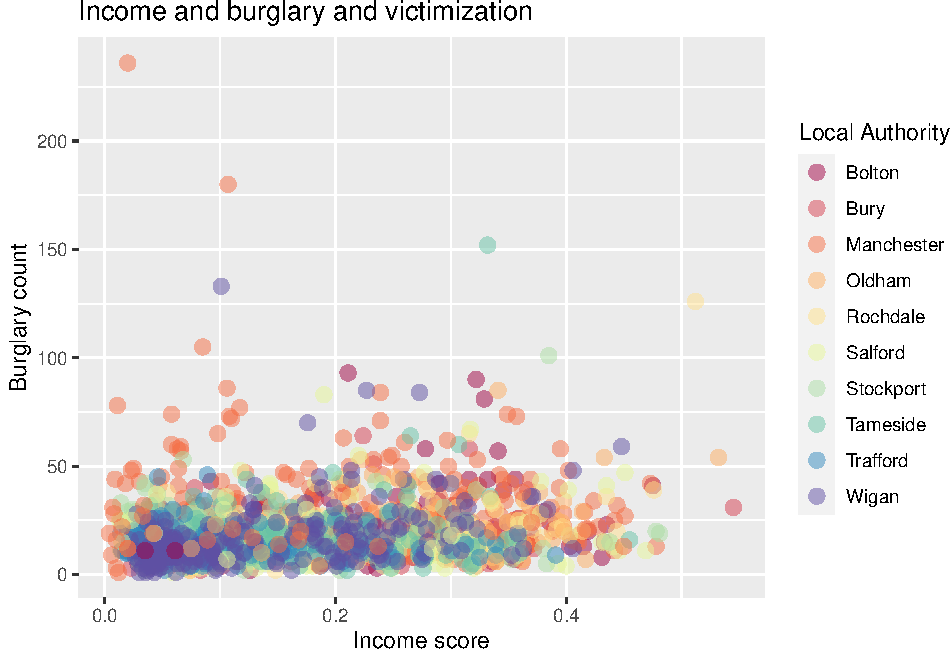
\includegraphics{03-data-visualisation_files/figure-latex/unnamed-chunk-11-1.pdf}

\begin{center}\rule{0.5\linewidth}{0.5pt}\end{center}

\hypertarget{activity-8-built-in-themes}{%
\subsubsection{Activity 8: Built-in Themes}\label{activity-8-built-in-themes}}

A final touch to your graphic can be the use of \textbf{themes}. These change the overall appearance of your graphic. The default theme we have for our graphic is \texttt{theme\_gray()}, but we can go for a minimalist look by using \texttt{theme\_minimal\ ()}. There are a number of these customised themes like one that is inspired by \emph{The Economist} ( \texttt{theme\_economist\ ()} ). To use special themes like \emph{The Economist}, install the package \texttt{ggthemes} and load it.

\begin{Shaded}
\begin{Highlighting}[]
\CommentTok{\# Changing graphic to the minimal theme with the last line of code}
\FunctionTok{ggplot}\NormalTok{(}\AttributeTok{data =}\NormalTok{ burglary\_df, }\AttributeTok{mapping =} \FunctionTok{aes}\NormalTok{(}\AttributeTok{x =}\NormalTok{ incscore, }\AttributeTok{y =}\NormalTok{ burglary\_count, }\AttributeTok{color =}\NormalTok{ LAname)) }\SpecialCharTok{+} 
  \FunctionTok{geom\_point}\NormalTok{(}\AttributeTok{size =} \DecValTok{3}\NormalTok{, }\AttributeTok{alpha =} \FloatTok{0.5}\NormalTok{) }\SpecialCharTok{+} 
  \FunctionTok{scale\_color\_brewer}\NormalTok{(}\AttributeTok{palette =} \StringTok{"Spectral"}\NormalTok{) }\SpecialCharTok{+} 
  \FunctionTok{labs}\NormalTok{(}\AttributeTok{x =} \StringTok{"Income score"}\NormalTok{, }\AttributeTok{y =} \StringTok{"Burglary count"}\NormalTok{, }\AttributeTok{title =} \StringTok{"Income and burglary and victimization"}\NormalTok{, }\AttributeTok{caption =} \StringTok{"Income score from 2019 IMD. Burglary counts from 2017."}\NormalTok{ , }\AttributeTok{color =} \StringTok{"Local Authority"}\NormalTok{) }\SpecialCharTok{+} 
  \FunctionTok{theme\_minimal}\NormalTok{()}
\end{Highlighting}
\end{Shaded}

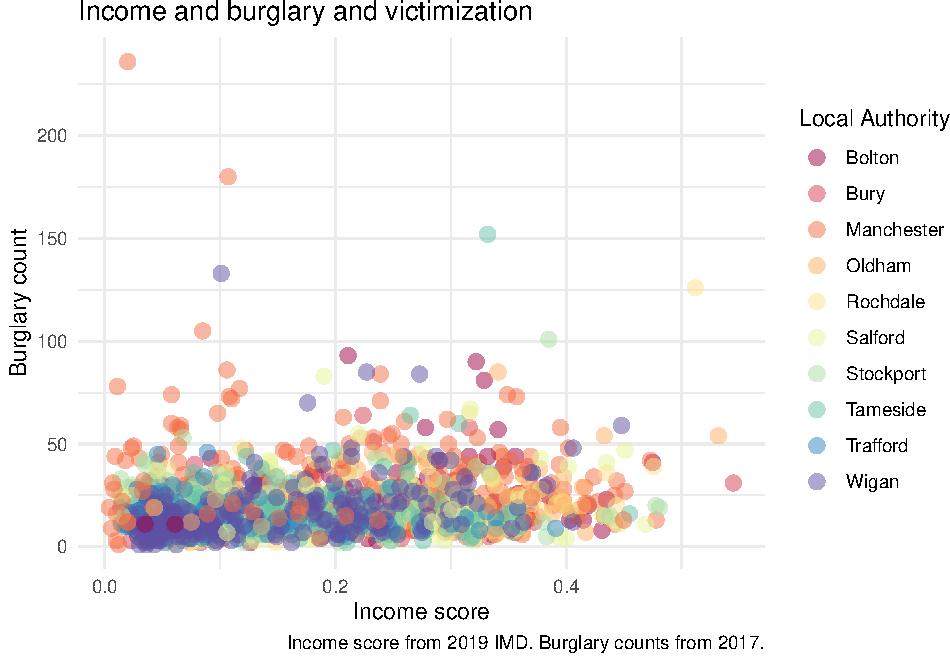
\includegraphics{03-data-visualisation_files/figure-latex/unnamed-chunk-12-1.pdf}

\begin{center}\rule{0.5\linewidth}{0.5pt}\end{center}

\hypertarget{graphs-for-categorical-data}{%
\subsection{Graphs for Categorical Data}\label{graphs-for-categorical-data}}

\hypertarget{activity-9-bar-graphs}{%
\subsubsection{Activity 9: Bar graphs}\label{activity-9-bar-graphs}}

To explore the count distribution of categorical variables, use the bar graph. We may be interested to know the number of neighbourhoods falling into each indice of the multiple deprivation (IMD) decile, a key indicator of criminality. Those in decile 1 are within the most deprived 10\% of LSOAs nationally; those in decile 10 are considered within the least deprived 10\% of LSOAs nationally.

The variable of interest, \texttt{IMDdeci}, is classed as numeric but we will need to treat it as a factor or else the default x-axis will include non-integer values like 7.5 .

Instead of making a new object, \texttt{ggplot} can calculate these frequencies by only specifying the x-axis and using the function \texttt{as.factor()}:

\begin{Shaded}
\begin{Highlighting}[]
\FunctionTok{ggplot}\NormalTok{(}\AttributeTok{data =}\NormalTok{ burglary\_df) }\SpecialCharTok{+} 
  \FunctionTok{geom\_bar}\NormalTok{(}\AttributeTok{mapping =} \FunctionTok{aes}\NormalTok{(}\AttributeTok{x =} \FunctionTok{as.factor}\NormalTok{(IMDdeci))) }\SpecialCharTok{+} \CommentTok{\# convert IMDdeci to a factor with as.factor }
  \FunctionTok{labs}\NormalTok{(}\AttributeTok{x =} \StringTok{"Deprivation Score"}\NormalTok{, }\AttributeTok{y =} \StringTok{"Number of Lower Super Output Areas"}\NormalTok{)}
\end{Highlighting}
\end{Shaded}

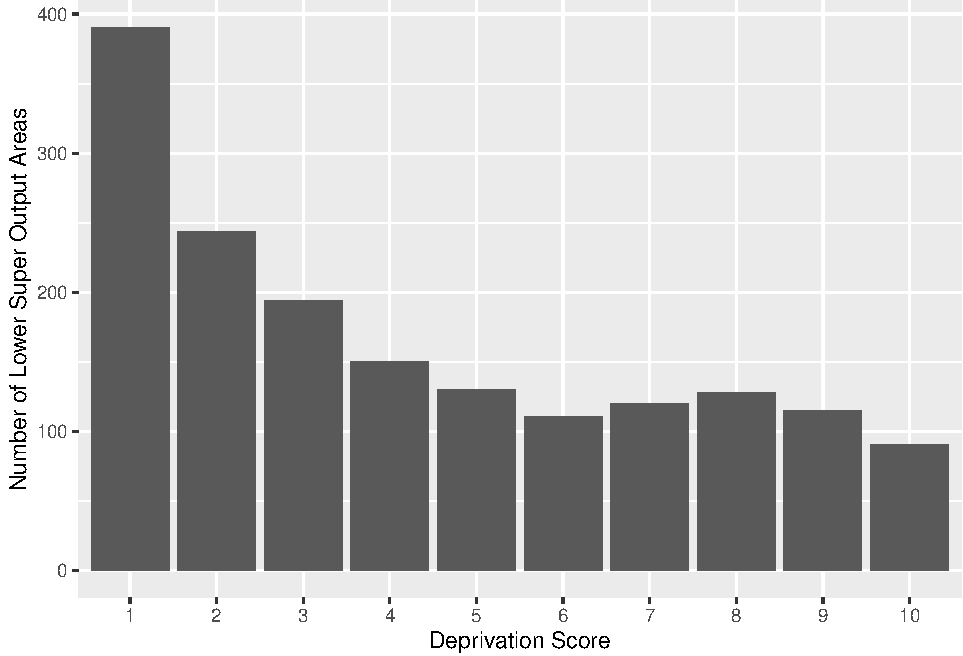
\includegraphics{03-data-visualisation_files/figure-latex/unnamed-chunk-13-1.pdf}

\hypertarget{grouped-bar-graphs}{%
\subsubsection{\texorpdfstring{\emph{Grouped Bar Graphs}}{Grouped Bar Graphs}}\label{grouped-bar-graphs}}

If we are interested in the distribution of deprivation like the previous bar graph but would like to see it by local authority, we can use the grouped bar graph, and specify the colour with the \texttt{fill\ =} parameter inside the \texttt{aes()} function.

Think back, however, to what we learned last semester, about row and column percentages, and how in bivariate analysis it is important to make decisions that will affect how our readers interpret our data. For example, if we fill the colour of each bar by local authority, we get a chart like this:

\begin{Shaded}
\begin{Highlighting}[]
\CommentTok{\# The ‘dodge’ position means that the bars avoid or ‘dodge’ each other}
\FunctionTok{ggplot}\NormalTok{(}\AttributeTok{data =}\NormalTok{ burglary\_df) }\SpecialCharTok{+} 
  \FunctionTok{geom\_bar}\NormalTok{(}\AttributeTok{mapping =} \FunctionTok{aes}\NormalTok{(}\AttributeTok{x =} \FunctionTok{as.factor}\NormalTok{(IMDdeci), }\AttributeTok{fill =}\NormalTok{ LAname), }\AttributeTok{position =} \StringTok{"stack"}\NormalTok{) }\SpecialCharTok{+}
  \FunctionTok{scale\_fill\_viridis\_d}\NormalTok{() }\SpecialCharTok{+} 
  \FunctionTok{labs}\NormalTok{(}\AttributeTok{x =} \StringTok{"Deprivation Score"}\NormalTok{, }\AttributeTok{y =} \StringTok{"Number of Lower Super Output Areas"}\NormalTok{, }\AttributeTok{fill =} \StringTok{"Local Authority"}\NormalTok{)}
\end{Highlighting}
\end{Shaded}

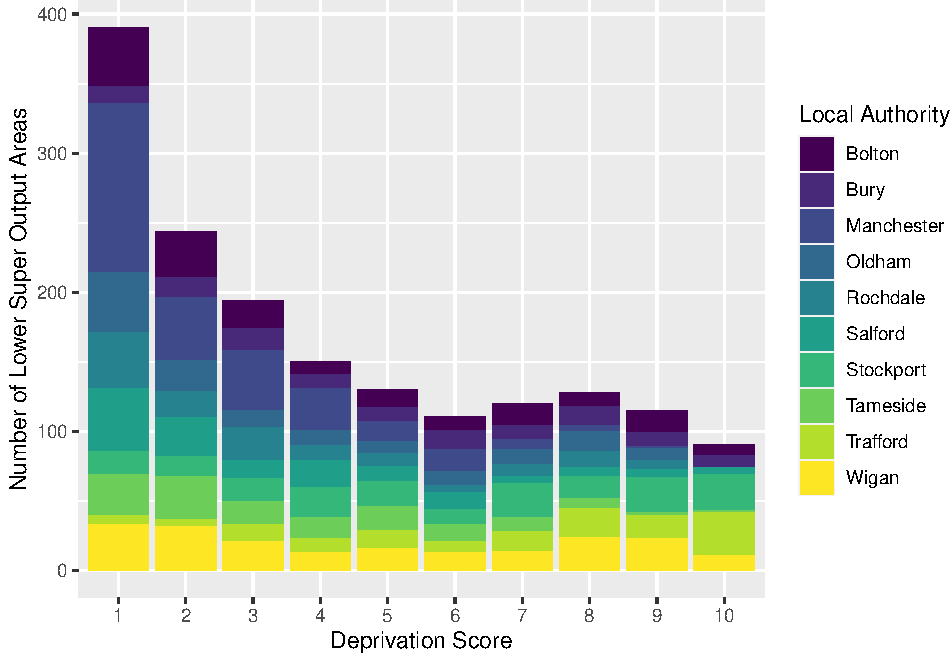
\includegraphics{03-data-visualisation_files/figure-latex/unnamed-chunk-14-1.pdf}

How do the different local authorities compare in terms of the distribution of deprived neighbourhoods? It can be a bit tough to say. But what about if we flip these:

\begin{Shaded}
\begin{Highlighting}[]
\CommentTok{\# We switch the positions of LAname and IMDdeci in the second line of code in this example}
\FunctionTok{ggplot}\NormalTok{(}\AttributeTok{data =}\NormalTok{ burglary\_df) }\SpecialCharTok{+} 
  \FunctionTok{geom\_bar}\NormalTok{(}\AttributeTok{mapping =} \FunctionTok{aes}\NormalTok{(}\AttributeTok{x =}\NormalTok{ LAname, }\AttributeTok{fill =} \FunctionTok{as.factor}\NormalTok{(IMDdeci)), }\AttributeTok{position =} \StringTok{"stack"}\NormalTok{) }\SpecialCharTok{+}
  \FunctionTok{scale\_fill\_viridis\_d}\NormalTok{() }\SpecialCharTok{+} 
  \FunctionTok{labs}\NormalTok{(}\AttributeTok{x =} \StringTok{"Local Authority"}\NormalTok{, }\AttributeTok{y =} \StringTok{"Number of Lower Super Output Areas"}\NormalTok{, }\AttributeTok{fill =} \StringTok{"Deprivation Score"}\NormalTok{)}
\end{Highlighting}
\end{Shaded}

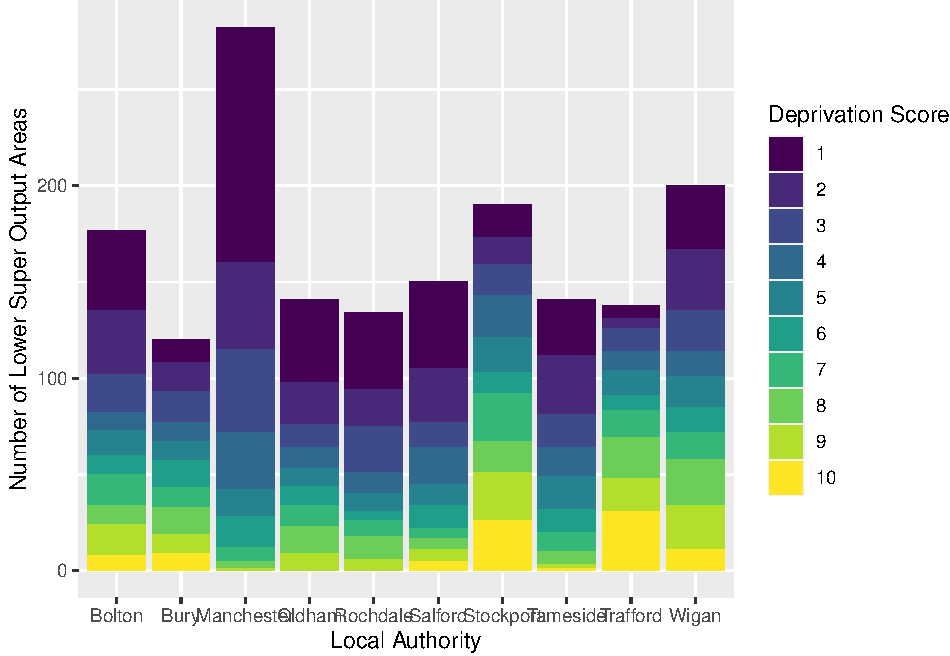
\includegraphics{03-data-visualisation_files/figure-latex/unnamed-chunk-15-1.pdf}

This seems clearer.

In your google doc, state what you observe from the bar graph and grouped bar graph depicting the relationship between deprivation and LSOAs.

\begin{center}\rule{0.5\linewidth}{0.5pt}\end{center}

\textbf{Note}: in the previous example, you might have noticed -- inside the \texttt{geom\_bar()} function, after the closing bracket of the \texttt{aes()} function -- the parameter \texttt{,\ position\ =\ "stack"}. This means that we get a \emph{stacked} bar chart. You could change this to \texttt{,\ position\ =\ "dodge"}, which would give you a clustered bar chart. Like so:

\begin{Shaded}
\begin{Highlighting}[]
\CommentTok{\# Instead of stack, the ‘dodge’ position means that the bars avoid or ‘dodge’ each other}
\FunctionTok{ggplot}\NormalTok{(}\AttributeTok{data =}\NormalTok{ burglary\_df) }\SpecialCharTok{+} 
  \FunctionTok{geom\_bar}\NormalTok{(}\AttributeTok{mapping =} \FunctionTok{aes}\NormalTok{(}\AttributeTok{x =}\NormalTok{ LAname, }\AttributeTok{fill =} \FunctionTok{as.factor}\NormalTok{(IMDdeci)), }\AttributeTok{position =} \StringTok{"dodge"}\NormalTok{) }\SpecialCharTok{+}
  \FunctionTok{scale\_fill\_viridis\_d}\NormalTok{() }\SpecialCharTok{+} 
  \FunctionTok{labs}\NormalTok{(}\AttributeTok{x =} \StringTok{"Local Authority"}\NormalTok{, }\AttributeTok{y =} \StringTok{"Number of Lower Super Output Areas"}\NormalTok{, }\AttributeTok{fill =} \StringTok{"Deprivation Score"}\NormalTok{)}
\end{Highlighting}
\end{Shaded}

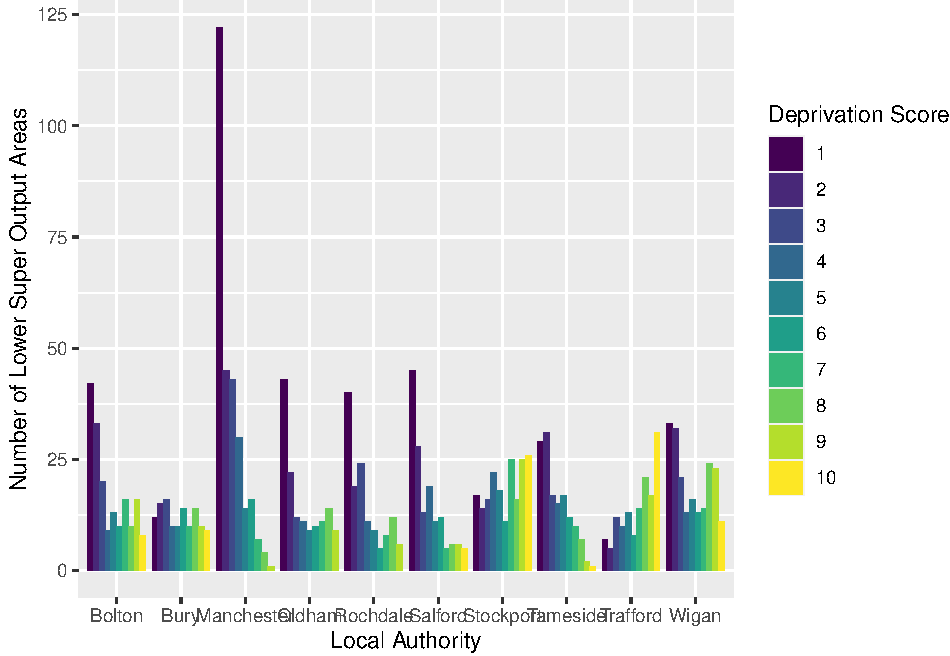
\includegraphics{03-data-visualisation_files/figure-latex/unnamed-chunk-16-1.pdf}

This might also be another way to display your data. There are advantages and disadvantages to both the stacked and clustered bar charts, and it has to do with what they hide and show!

\begin{center}\rule{0.5\linewidth}{0.5pt}\end{center}

\hypertarget{multiple-bar-graphs}{%
\subsubsection{\texorpdfstring{\emph{Multiple Bar Graphs}}{Multiple Bar Graphs}}\label{multiple-bar-graphs}}

Another useful visual is multiple bar graphs. This creates different plots for each level of a factor instead of putting lots of information into one graphic. Using the function \texttt{facet\_wrap\ ()}, we make the information obtained from the previous scatterplot, where we coloured in each point by local authority, clearer.

Although the scatterplot uses numeric variables, we use this information by local authority, and \texttt{LAname} is classed as factor:

\begin{Shaded}
\begin{Highlighting}[]
\CommentTok{\# To facet the scatterplot by local authority, ‘ \textasciitilde{} ‘ is used next to ‘LAname’}
\FunctionTok{ggplot}\NormalTok{(}\AttributeTok{data =}\NormalTok{ burglary\_df) }\SpecialCharTok{+} 
  \FunctionTok{geom\_point}\NormalTok{(}\AttributeTok{mapping =} \FunctionTok{aes}\NormalTok{(}\AttributeTok{x =}\NormalTok{ incscore, }\AttributeTok{y =}\NormalTok{ burglary\_count)) }\SpecialCharTok{+} 
  \FunctionTok{facet\_wrap}\NormalTok{(}\SpecialCharTok{\textasciitilde{}}\NormalTok{LAname)}
\end{Highlighting}
\end{Shaded}

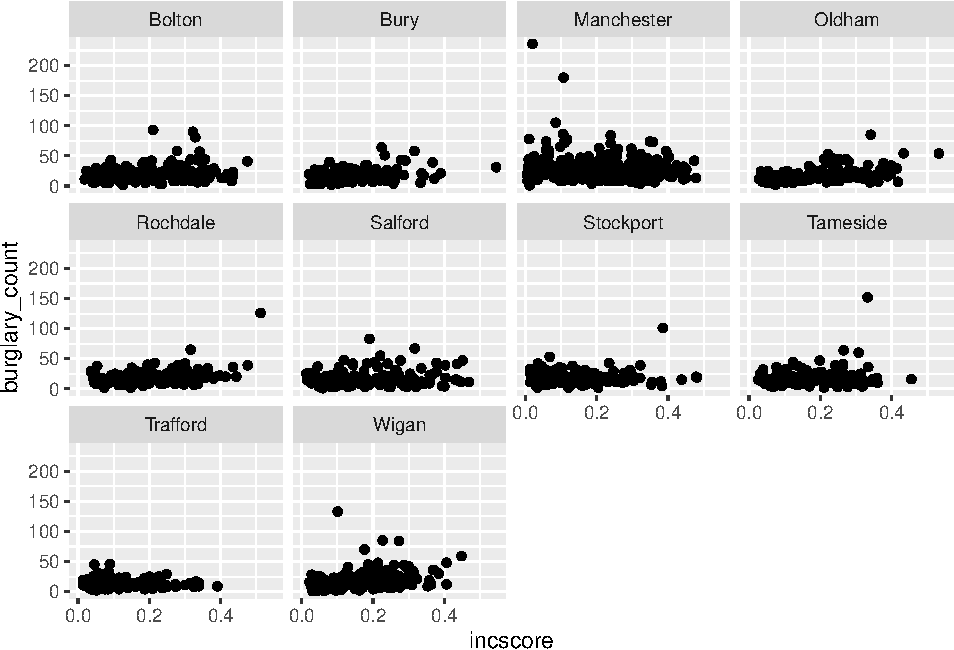
\includegraphics{03-data-visualisation_files/figure-latex/unnamed-chunk-17-1.pdf}

\begin{Shaded}
\begin{Highlighting}[]
\CommentTok{\# By default, facet\_wrap fixes the y{-}axis of each graph to make comparisons easier}
\end{Highlighting}
\end{Shaded}

It is important to choose an appropriate graph, so thought is required. May the following graphic be fair warning:

\begin{figure}
\centering
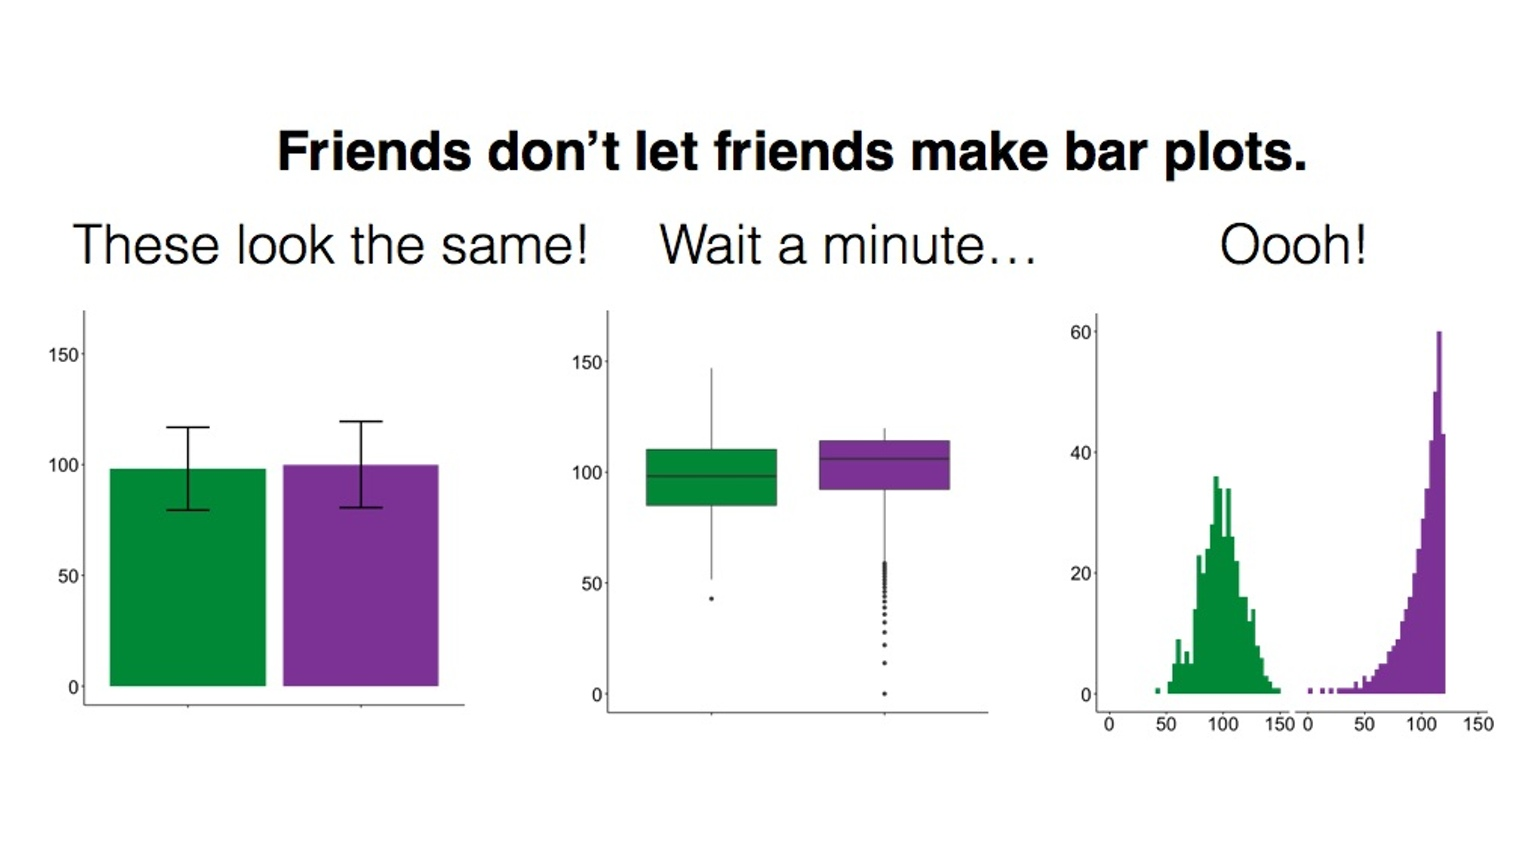
\includegraphics{Images/barplots.jpg}
\caption{\textbf{Figure 3.8} Friends don't let friends do this}
\end{figure}

\begin{center}\rule{0.5\linewidth}{0.5pt}\end{center}

\hypertarget{graphs-for-numeric-data}{%
\subsection{Graphs for Numeric Data}\label{graphs-for-numeric-data}}

\hypertarget{activity-10-histograms}{%
\subsubsection{Activity 10: Histograms}\label{activity-10-histograms}}

Histograms differ from scatterplots because they require only one numeric variable and they create bins, visualized as bars, to count the frequency of each bar. We create a histogram of the variable \texttt{IMDscore}, the overall score of deprivation in each neighbourhood:

\begin{Shaded}
\begin{Highlighting}[]
\FunctionTok{ggplot}\NormalTok{(}\AttributeTok{data =}\NormalTok{ burglary\_df, }\AttributeTok{mapping =} \FunctionTok{aes}\NormalTok{(}\AttributeTok{x =}\NormalTok{ IMDscore)) }\SpecialCharTok{+} 
  \FunctionTok{geom\_histogram}\NormalTok{()}
\end{Highlighting}
\end{Shaded}

\begin{verbatim}
## `stat_bin()` using `bins = 30`. Pick better value with `binwidth`.
\end{verbatim}

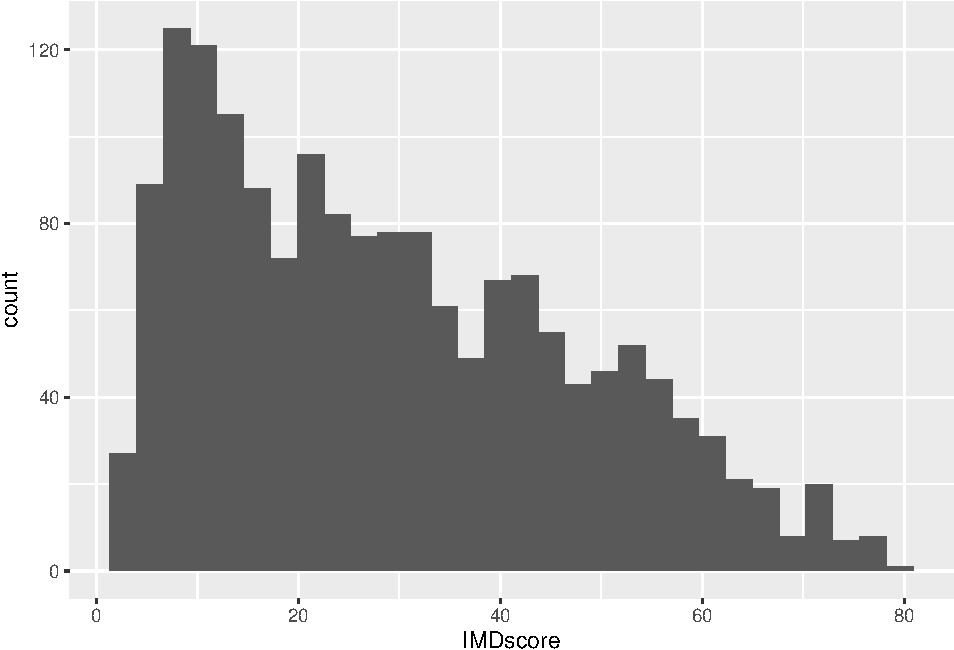
\includegraphics{03-data-visualisation_files/figure-latex/unnamed-chunk-18-1.pdf}

How the histogram looks, and therefore, the conclusions drawn from the visual, are sensitive to the number of \textbf{bins}. You should try different specifications of the bin-width until you find one that tells the complete and concise story of the data. Specifying the size of bins is done using the argument \texttt{bin\_width\ =}; the default size is 30 and you can change this to get a rougher or a more granular idea:

\begin{Shaded}
\begin{Highlighting}[]
\CommentTok{\# Using bin{-}width of 1 we are essentially creating a bar for every increase in level of deprivation}
\FunctionTok{ggplot}\NormalTok{(}\AttributeTok{data =}\NormalTok{ burglary\_df, }\AttributeTok{mapping =} \FunctionTok{aes}\NormalTok{(}\AttributeTok{x =}\NormalTok{ IMDscore)) }\SpecialCharTok{+} 
  \FunctionTok{geom\_histogram}\NormalTok{(}\AttributeTok{binwidth =} \DecValTok{1}\NormalTok{)}
\end{Highlighting}
\end{Shaded}

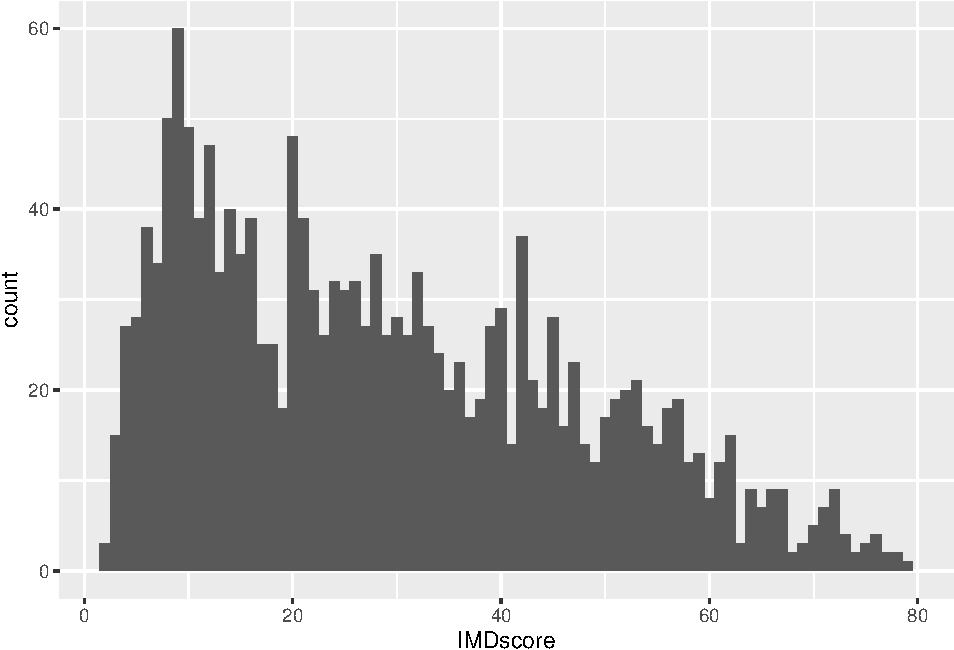
\includegraphics{03-data-visualisation_files/figure-latex/unnamed-chunk-19-1.pdf}

Play around with the bin widths to find which one looks the most visually comprehensible. In your google doc, state what bin width you think does the job, and why.

\begin{center}\rule{0.5\linewidth}{0.5pt}\end{center}

\hypertarget{activity-11-line-graphs}{%
\subsubsection{Activity 11: Line Graphs}\label{activity-11-line-graphs}}

A very good way of visualizing trends over time are line graphs. For this, let us use the \texttt{monthly\_df} data frame. Ensure it is loaded into your environment. Have a look at the structure of these data to get to know them.

The data is in long format: we have a single month variable for 12 months' worth of data (rather than one variable or column for each month). Setting longitudinal data up in long format allows us to specify the aesthetics (e.g., x- and y-axes) easily.

For a line graph, we use the function \texttt{geom\_line()}. We plan to plot the counts to show the trends of different crimes over the course of the year. Our time variable, \texttt{month}, should run along the x-axis, and the count variable, \texttt{n}, should run on the y-axis.

To show each crime type separately, we use the group aesthetic and a new aesthetic, \texttt{linetype}, which uses different patterns for each group. To show our time measurement points, we also add \texttt{geom\_point\ ()}:

\begin{Shaded}
\begin{Highlighting}[]
\FunctionTok{ggplot}\NormalTok{(}\AttributeTok{data =}\NormalTok{ monthly\_df, }\FunctionTok{aes}\NormalTok{(}\AttributeTok{x =} \FunctionTok{as.factor}\NormalTok{(Month), }\AttributeTok{y =}\NormalTok{ n, }\AttributeTok{group =}\NormalTok{ crime\_type, }\AttributeTok{linetype =}\NormalTok{ crime\_type)) }\SpecialCharTok{+} 
  \FunctionTok{geom\_line}\NormalTok{() }\SpecialCharTok{+} 
  \FunctionTok{geom\_point}\NormalTok{()}
\end{Highlighting}
\end{Shaded}

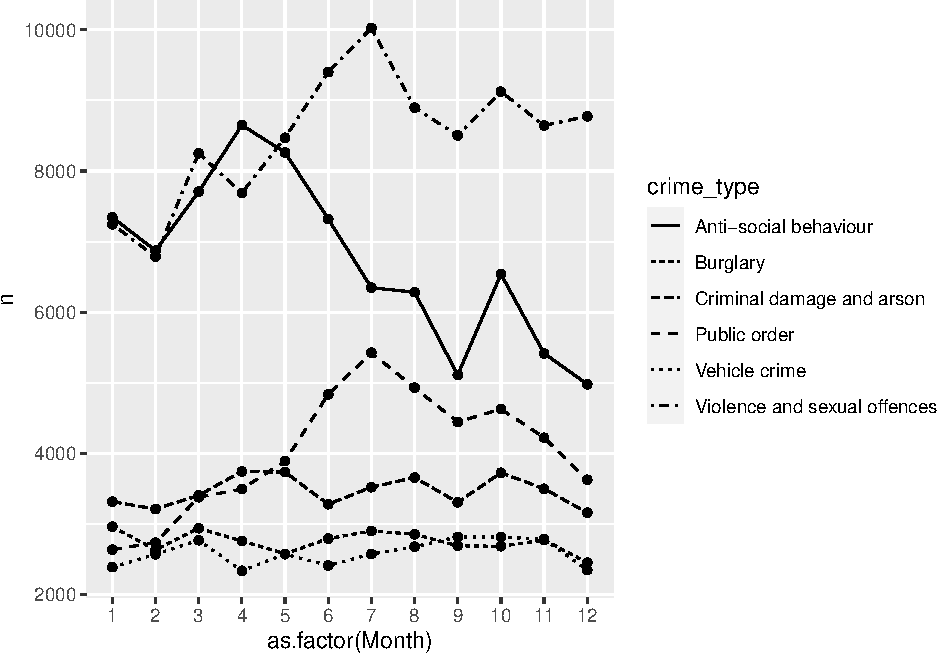
\includegraphics{03-data-visualisation_files/figure-latex/unnamed-chunk-20-1.pdf}

\begin{Shaded}
\begin{Highlighting}[]
\CommentTok{\# We are saying, ‘Hey R, may you please make a graphic using the data frame “monthly\_df”, and map the variable “month” (turning it into a factor) to the x{-}axis and “n” to the y{-}axis, and group this information by “crime\_type”, showing different patterns for each crime type, then pass this information through (“ +”) to make a line graph, and pass this information through (“ +”) to make a scatterplot of the time points too?’}
\end{Highlighting}
\end{Shaded}

Now, in your google doc, state what you observe from this line graph on different crimes throughout the months.

\begin{center}\rule{0.5\linewidth}{0.5pt}\end{center}

\hypertarget{activity-12-boxplots}{%
\subsubsection{Activity 12: Boxplots}\label{activity-12-boxplots}}

If you want more information about your data than a histogram can give, a box (and whisker) plot may be what you are looking for. A boxplot visualizes the minimum, maximum, interquartile range, the median, and any unusual observations - your five-number summary!

For this example, we return to the \texttt{burglary\_df} data, and focus on the distribution of burglary counts. In addition, we make a boxplot for \emph{each} deprivation decile to show how LSOAs in the most deprived deciles often have higher median burglary counts.

We send all of this information, the boxplots, into one object called \texttt{my\_whisker\_plot}, to which we can return in case:

\begin{Shaded}
\begin{Highlighting}[]
\NormalTok{my\_whisker\_plot }\OtherTok{\textless{}{-}} \FunctionTok{ggplot}\NormalTok{(}\AttributeTok{data =}\NormalTok{ burglary\_df) }\SpecialCharTok{+} 
\FunctionTok{geom\_boxplot}\NormalTok{(}\AttributeTok{mapping =} \FunctionTok{aes}\NormalTok{(}\AttributeTok{x =} \FunctionTok{as.factor}\NormalTok{(IMDdeci), }\AttributeTok{y =}\NormalTok{ burglary\_count, }\AttributeTok{group =} \FunctionTok{as.factor}\NormalTok{(IMDdeci), }\AttributeTok{fill =} \FunctionTok{as.factor}\NormalTok{(IMDdeci))) }

\NormalTok{my\_whisker\_plot }\SpecialCharTok{+} 
  \FunctionTok{labs}\NormalTok{(}\AttributeTok{x =} \StringTok{"Deprivation Scale"}\NormalTok{, }\AttributeTok{y =} \StringTok{"Number of Burglaries"}\NormalTok{)}
\end{Highlighting}
\end{Shaded}

\includegraphics{03-data-visualisation_files/figure-latex/unnamed-chunk-21-1.pdf}

In your group google doc, state what you observe from your newly created boxplot.

\begin{center}\rule{0.5\linewidth}{0.5pt}\end{center}

\hypertarget{summary-2}{%
\section{SUMMARY}\label{summary-2}}

Today was about using a popular package called \texttt{ggplot2} for effectively visualizing data. We learn this because it is important to understand our data before embarking on more complex analyses. If we do not understand our data beforehand, we risk misinterpreting what the data are trying to tell us. The package is based on this approach called \emph{Grammar of Graphics}, which proposes a `grammar' to describe and construct statistical graphics. The package, however, sees the creation of data visuals accomplished through \textbf{layers}.

Our first topic we learned was about these layers, comprising data, aesthetics, and geometric objects. As a final touch, \textbf{themes} changed the overall appearance of your graphic. Our second and third topics introduced us to \textbf{graphs} that we can use for all types of variables, and how to create them in \texttt{ggplot2}. One example was the histogram, whereby adjusting the width of the \textbf{bins} helped for better interpretation of the data.

Hurrah: homework time!

\hypertarget{answers-to-activities}{%
\subsection{ANSWERS TO ACTIVITIES:}\label{answers-to-activities}}

\begin{itemize}
\item
  \begin{enumerate}
  \def\labelenumi{\arabic{enumi}.}
  \tightlist
  \item
    burglary\_df: 1,673 observations, 9 variables ; monthly\_df: 73 observations, 3 variables
  \end{enumerate}
\item
  \begin{enumerate}
  \def\labelenumi{\arabic{enumi}.}
  \setcounter{enumi}{1}
  \item
    \begin{enumerate}
    \def\labelenumii{(\arabic{enumii})}
    \tightlist
    \item
      burglary\_df: n= 1,673 LSOAs; (2) monthly\_df: n= 72 months
    \end{enumerate}
  \end{enumerate}
\item
  \begin{enumerate}
  \def\labelenumi{\arabic{enumi}.}
  \setcounter{enumi}{2}
  \tightlist
  \item
    Hard to say\ldots{}
  \end{enumerate}
\item
  \begin{enumerate}
  \def\labelenumi{\arabic{enumi}.}
  \setcounter{enumi}{3}
  \tightlist
  \item
    Roughly: most areas have burglary counts below 50
  \end{enumerate}
\item
  \begin{enumerate}
  \def\labelenumi{\arabic{enumi}.}
  \setcounter{enumi}{4}
  \tightlist
  \item
    N/A
  \end{enumerate}
\item
  \begin{enumerate}
  \def\labelenumi{\arabic{enumi}.}
  \setcounter{enumi}{5}
  \tightlist
  \item
    N/A
  \end{enumerate}
\item
  \begin{enumerate}
  \def\labelenumi{\arabic{enumi}.}
  \setcounter{enumi}{6}
  \tightlist
  \item
    N/A
  \end{enumerate}
\item
  \begin{enumerate}
  \def\labelenumi{\arabic{enumi}.}
  \setcounter{enumi}{7}
  \tightlist
  \item
    N/A
  \end{enumerate}
\item
  \begin{enumerate}
  \def\labelenumi{\arabic{enumi}.}
  \setcounter{enumi}{8}
  \tightlist
  \item
    Roughly: The most number of LSOAs are in decile 1, meaning they are within the 10\% of the most deprived LSOAS, and in the final and stacked grouped bar graph, LSOAs from Manchester have a large number in decile 1.
  \end{enumerate}
\item
  \begin{enumerate}
  \def\labelenumi{\arabic{enumi}.}
  \setcounter{enumi}{9}
  \tightlist
  \item
    N/A
  \end{enumerate}
\item
  \begin{enumerate}
  \def\labelenumi{\arabic{enumi}.}
  \setcounter{enumi}{10}
  \tightlist
  \item
    Roughly: Violence and sexual offences are the highest compared to other crimes and reaches its peak in the summer months. Antisocial behaviour rises from February to April, then declines, hitting a low point in September before rising again.
  \end{enumerate}
\item
  \begin{enumerate}
  \def\labelenumi{\arabic{enumi}.}
  \setcounter{enumi}{11}
  \tightlist
  \item
    Roughly: Decile 1 has highest median (about 25) compared to other deciles but with many outliers. Decile 4 has the most extreme outlier of about 250 burglaries.
  \end{enumerate}
\end{itemize}

\hypertarget{descriptive-statistics}{%
\chapter{Descriptive Statistics}\label{descriptive-statistics}}

\hypertarget{central-tendency-outliers-and-dispersion}{%
\subsubsection*{\texorpdfstring{\emph{Central Tendency, Outliers, and Dispersion}}{Central Tendency, Outliers, and Dispersion}}\label{central-tendency-outliers-and-dispersion}}
\addcontentsline{toc}{subsubsection}{\emph{Central Tendency, Outliers, and Dispersion}}

\hypertarget{learning-outcomes-3}{%
\paragraph*{\texorpdfstring{\textbf{Learning Outcomes}}{Learning Outcomes}}\label{learning-outcomes-3}}
\addcontentsline{toc}{paragraph}{\textbf{Learning Outcomes}}

\begin{itemize}
\tightlist
\item
  Revisit what descriptive statistics are and their importance in understanding your data
\item
  Learn / review measures of the central tendency and dispersion and how to conduct them
\item
  Learn how to identify outliers and skewness
\end{itemize}

\hypertarget{todays-learning-tools-3}{%
\paragraph*{\texorpdfstring{\textbf{Today's Learning Tools:}}{Today's Learning Tools:}}\label{todays-learning-tools-3}}
\addcontentsline{toc}{paragraph}{\textbf{Today's Learning Tools:}}

\hypertarget{total-number-of-activities-12-1}{%
\paragraph*{\texorpdfstring{\emph{Total number of activities}: 12}{Total number of activities: 12}}\label{total-number-of-activities-12-1}}
\addcontentsline{toc}{paragraph}{\emph{Total number of activities}: 12}

\hypertarget{data-3}{%
\paragraph*{\texorpdfstring{\emph{Data:}}{Data:}}\label{data-3}}
\addcontentsline{toc}{paragraph}{\emph{Data:}}

\begin{itemize}
\tightlist
\item
  Law Enforcement Management and Administrative Statistics (LEMAS)-Body-Worn Camera Supplement (BWCS) Survey
\item
  2004 Survey of Inmates in State and Federal Correctional Facilities (SISFCF)
\end{itemize}

\hypertarget{packages-4}{%
\paragraph*{\texorpdfstring{\emph{Packages:}}{Packages:}}\label{packages-4}}
\addcontentsline{toc}{paragraph}{\emph{Packages:}}

\begin{itemize}
\tightlist
\item
  \texttt{dplyr}
\item
  \texttt{ggplot2}
\item
  \texttt{here}
\item
  \texttt{modeest}
\item
  \texttt{moments}
\item
  \texttt{qualvar}
\item
  \texttt{skimr}
\end{itemize}

\hypertarget{functions-introduced-and-packages-to-which-they-belong-3}{%
\paragraph*{\texorpdfstring{\emph{Functions introduced (and packages to which they belong)}}{Functions introduced (and packages to which they belong)}}\label{functions-introduced-and-packages-to-which-they-belong-3}}
\addcontentsline{toc}{paragraph}{\emph{Functions introduced (and packages to which they belong)}}

\begin{itemize}
\tightlist
\item
  \texttt{diff()} : Computes differences between values in a numeric vector (\texttt{base\ R})
\item
  \texttt{dim()} : Check the dimensions of an \texttt{R} object (\texttt{base\ R})
\item
  \texttt{DM()} : Computes deviation from the mode (\texttt{qualvar})
\item
  \texttt{group\_by()} : Group observations by variable(s) for performing operations (\texttt{dplyr})
\item
  \texttt{IQR()} : Compute interquartile range (\texttt{base\ R})
\item
  \texttt{is.na()} : Returns \texttt{TRUE} when values are missing, \texttt{FALSE} if not (\texttt{base\ R})
\item
  \texttt{load()} : Reads data that are stored in an \texttt{R} data file formet (\texttt{base\ R})
\item
  \texttt{mean()} : Compute arithmetic mean (\texttt{base\ R})
\item
  \texttt{max()} : Returns the maximum value (\texttt{base\ R})
\item
  \texttt{min()} : Returns the minimum value (\texttt{base\ R})
\item
  \texttt{mlv()} : Compute the mode (\texttt{modeest})
\item
  \texttt{quantile()} : Compute quantiles as per specified probabilities (\texttt{base\ R})
\item
  \texttt{sd()} : Computes standard deviation of a numeric vector (\texttt{base\ R})
\item
  \texttt{skewness()} : Calculate degree of skewness in a numeric vector (\texttt{modeest})
\item
  \texttt{skim()} : Provide summary statistics specific to object class (\texttt{skimr})
\item
  \texttt{summarize()} : Create new summary variable(s), e.g., counts, mean (\texttt{dplyr})
\item
  \texttt{summary()} : Produce summary of model results (\texttt{base\ R})
\item
  \texttt{table()} : Generates a frequency table (\texttt{base\ R})
\item
  \texttt{var()} : Computes variance (\texttt{base\ R})
\end{itemize}

\begin{center}\rule{0.5\linewidth}{0.5pt}\end{center}

\hypertarget{revisiting-descriptive-statistics}{%
\section{Revisiting Descriptive Statistics}\label{revisiting-descriptive-statistics}}

The field of statistics is divided into two main branches: descriptive and inferential. Much of what you will cover today on descriptive statistics will be a review from last semester, but learning to conduct them in \texttt{R} will be a new learning experience.

So, what are descriptive statistics? If general statistics is concerned with the study of how best to collect, analyse, and make conclusions about data, then this specific branch -- descriptive statistics -- is concerned with the sample distribution and the population distribution from which the sample is drawn. Basically, descriptive statistics are ways of describing your data.

Similar to last week's lesson on data visualization, describing your data is important because it helps you identify patterns and anomalies. In addition, it gives others a succinct understanding of your data, so it facilitates good communication. We revisit and learn another three substantive topics today: the \textbf{central tendency}, \textbf{outliers}, and \textbf{dispersion}.

\hypertarget{activity-1-our-preparation-routine}{%
\subsection{Activity 1: Our preparation routine}\label{activity-1-our-preparation-routine}}

We start by doing the usual routine, but with new data on police body-worn cameras:

\begin{enumerate}
\def\labelenumi{\arabic{enumi}.}
\item
  Open up your existing \texttt{R} project
\item
  Load the required packages (listed at the top of this lesson). Some of these are familiar from previous weeks, so you only need to use the function \texttt{library()}to load them. For packages that we have not used before and are not installed in our \texttt{R}, you will need to use the function \texttt{install.packages()} first before loading it with \texttt{library()}:
\end{enumerate}

\begin{Shaded}
\begin{Highlighting}[]
\CommentTok{\# Remember, we only need to do this once whenever we meet a new package and would like to keep it handy in our own R library of packages:}

\FunctionTok{install.packages}\NormalTok{(}\StringTok{"modeest"}\NormalTok{)}
\FunctionTok{install.packages}\NormalTok{(}\StringTok{"moments"}\NormalTok{)}
\FunctionTok{install.packages}\NormalTok{(}\StringTok{"qualvar"}\NormalTok{)}
\FunctionTok{install.packages}\NormalTok{(}\StringTok{"skimr"}\NormalTok{)}
\end{Highlighting}
\end{Shaded}

\begin{Shaded}
\begin{Highlighting}[]
\CommentTok{\# All of these are now in our R library of packages, but we need to load them, or \textquotesingle{}bring them to life\textquotesingle{}, to use their functions:}

\FunctionTok{library}\NormalTok{(dplyr)}
\FunctionTok{library}\NormalTok{(ggplot2)}
\FunctionTok{library}\NormalTok{(here)}
\FunctionTok{library}\NormalTok{(modeest)}
\FunctionTok{library}\NormalTok{(moments)}
\FunctionTok{library}\NormalTok{(qualvar)}
\FunctionTok{library}\NormalTok{(skimr)}
\end{Highlighting}
\end{Shaded}

\begin{enumerate}
\def\labelenumi{\arabic{enumi}.}
\setcounter{enumi}{2}
\item
  You will have downloaded the datasets from Blackboard as usual, ensuring the datasets have been moved into the subfolder you had created from Lesson 2 called `Datasets'.
\item
  For now, open only the 2016 LEMAS-BWCS dataset (37302-0001-Data.rda). These data are from the \href{https://www.icpsr.umich.edu/web/pages/}{Inter-university Consortium for Political and Social Research (ICPSR) website} and you can find them by using the dataset name, which refers to the ICPSR study number. This time, data are stored in an \texttt{R} data file format (.rda). Always check for the type of file format the data are in - this determines what codes and packages (if any) you will need to use to load the data into \texttt{R}.
\item
  For this type of dataset, as it is in an `.rda' data file format, we will need to use the \texttt{load()} function to import the data frame into our environment, specifying your working directory using \texttt{here()} like we have in Lesson 2, section 2.1.
\end{enumerate}

\begin{Shaded}
\begin{Highlighting}[]
\FunctionTok{load}\NormalTok{(}\FunctionTok{here}\NormalTok{(}\StringTok{"Datasets"}\NormalTok{, }\StringTok{"37302{-}0001{-}Data.rda"}\NormalTok{))}
\end{Highlighting}
\end{Shaded}

\begin{enumerate}
\def\labelenumi{\arabic{enumi}.}
\setcounter{enumi}{5}
\tightlist
\item
  Name the data frame \texttt{bwcs} by using the \texttt{\textless{}-} assignment operator. Another way of looking at it is you are putting the dataset into a `box' that you will call `bwcs'. It will appear in the Environment pane like all objects you create in \texttt{R}.
\end{enumerate}

\begin{Shaded}
\begin{Highlighting}[]
\NormalTok{bwcs }\OtherTok{\textless{}{-}}\NormalTok{ da37302}\FloatTok{.0001}
\end{Highlighting}
\end{Shaded}

\begin{enumerate}
\def\labelenumi{\arabic{enumi}.}
\setcounter{enumi}{6}
\tightlist
\item
  Use the function \texttt{View(bwcs)} to ensure the file is loaded and to get to know your data. You can also use the function \texttt{dim(bwcs)} to see the number of observations and variables.
\end{enumerate}

\begin{center}\rule{0.5\linewidth}{0.5pt}\end{center}

\hypertarget{todays-3-1}{%
\section{Today's 3}\label{todays-3-1}}

Two primary ways of describing your data have to do with the central tendency and their dispersion. We also learn about outliers.

\begin{center}\rule{0.5\linewidth}{0.5pt}\end{center}

\hypertarget{central-tendency}{%
\subsection{Central Tendency}\label{central-tendency}}

Central tendency refers to a descriptive summary of the centre of the data's distribution; it takes the form of a single number that is meant to represent the middle or average of the data. The \textbf{mean}, \textbf{median}, and \textbf{mode} are common statistics of the central tendency.

The \emph{mean} is the average and it is useful when we want to summarise a variable quickly. Its disadvantage is that it is sensitive to extreme values, so the mean can be distorted easily.

To address this sensitivity, the \emph{median} is a better measure because it is a robust estimate, which means that it is not easily swayed by extreme values. It is the middle value of the distribution.

The \emph{mode} helps give an idea of what is the most typical value in the distribution, which is the most frequently occurring case in the data. While mean and median apply to numeric variables, the mode is most useful when describing categorical variables. For example, you may want to know the most frequently occurring category.

\hypertarget{activity-2-recap-of-how-to-obtain-the-mean-and-median}{%
\subsubsection{Activity 2: Recap of how to obtain the mean and median}\label{activity-2-recap-of-how-to-obtain-the-mean-and-median}}

In Lesson 1, you were introduced to the functions \texttt{mean()} and \texttt{median()}. There is no direct function in \texttt{base\ R} to calculate the mode, but we will learn one way to do so soon. First, find only the mean and median for the following six numbers:

\begin{Shaded}
\begin{Highlighting}[]
\CommentTok{\# 345, 100, 250, 100, 101, 300 }
\end{Highlighting}
\end{Shaded}

Type your answers in the group google doc.

\begin{center}\rule{0.5\linewidth}{0.5pt}\end{center}

\hypertarget{activity-3-levels-of-measurement}{%
\subsubsection{Activity 3: Levels of measurement}\label{activity-3-levels-of-measurement}}

From today's data, we are interested in exploring the adoption of body-worn cameras (BWCs) and their usage in a sample of agencies. The variables that will help us explore this is \texttt{Q\_10A} because it measures whether the agency adopted BWCs as of 2016 and \texttt{Q\_12} because it measures the number of cameras that agencies reported using.

Let us say we want to learn about these variables. The first step to choosing the appropriate analysis for our variables, \texttt{Q\_10A} and \texttt{Q\_12}, is establishing: \emph{what are their levels of measurement}?

To review levels of measurement, refer to Lesson 2 (section 2.4.1). Have a think and record your answers for each variable in the google doc.

\url{....}

\textbf{Figure 4.1} What are the levels of measurement?

Now that we have established the level of measurement for our variables, what type of object does \texttt{R} think these variables are? In other words, what are these variables classed as? Recall that we can use the \texttt{class()} function to answer this:

\begin{Shaded}
\begin{Highlighting}[]
\CommentTok{\# We start with variable Q\_10A:}

\FunctionTok{class}\NormalTok{(bwcs}\SpecialCharTok{$}\NormalTok{Q\_10A) }
\end{Highlighting}
\end{Shaded}

\begin{verbatim}
## [1] "factor"
\end{verbatim}

\texttt{Q\_10A} is classed as a factor. Another function that will return what the variable is classed as but also the specific levels is the \texttt{attributes()} function:

\begin{Shaded}
\begin{Highlighting}[]
\FunctionTok{attributes}\NormalTok{(bwcs}\SpecialCharTok{$}\NormalTok{Q\_10A)}
\end{Highlighting}
\end{Shaded}

\begin{verbatim}
## $levels
## [1] "(1) Agency has acquired in any form (including testing)"
## [2] "(2) Agency has not acquired"                            
## 
## $class
## [1] "factor"
\end{verbatim}

This factor variable has two levels: `(1) Agency has acquired in any form (including testing)' and `(2) Agency has not acquired'.

Now, we want to know the \textbf{mode} -- which level or category appears most frequently in our data set. We use the function \texttt{mlv()} (acronym for \textbf{m}ost \textbf{l}ikely \textbf{v}alues) from the \texttt{modeest} package to answer this question:

\begin{Shaded}
\begin{Highlighting}[]
\CommentTok{\# Double check that the package modeest is loaded for this code to work}

\FunctionTok{mlv}\NormalTok{(bwcs}\SpecialCharTok{$}\NormalTok{Q\_10A)}
\end{Highlighting}
\end{Shaded}

\begin{verbatim}
## [1] (2) Agency has not acquired
## 2 Levels: (1) Agency has acquired in any form (including testing) ...
\end{verbatim}

The output returns the answer as: `(2) Agency has not acquired'. It also, conveniently, prints all the levels so we can see what are the other categories.

If you want to cross check your answer obtained from the \texttt{mlv()} function, create a frequency table using the \texttt{table()} function:

\begin{Shaded}
\begin{Highlighting}[]
\FunctionTok{table}\NormalTok{(bwcs}\SpecialCharTok{$}\NormalTok{Q\_10A)}
\end{Highlighting}
\end{Shaded}

\begin{verbatim}
## 
## (1) Agency has acquired in any form (including testing) 
##                                                    1915 
##                             (2) Agency has not acquired 
##                                                    2013
\end{verbatim}

Indeed, there are 2,013 observations where the agency had not acquired any body worn cameras, which is more than the 1,915 observations where the agency had acquired body worn cameras in any format.

We could also run the \texttt{mlv()} function and save the output in an object rather than print the answers into the console. Here, we save to the object called \texttt{mode\_adopted}:

\begin{Shaded}
\begin{Highlighting}[]
\NormalTok{mode\_adopted }\OtherTok{\textless{}{-}} \FunctionTok{mlv}\NormalTok{(bwcs}\SpecialCharTok{$}\NormalTok{Q\_10A) }
\NormalTok{mode\_adopted}
\end{Highlighting}
\end{Shaded}

\begin{verbatim}
## [1] (2) Agency has not acquired
## 2 Levels: (1) Agency has acquired in any form (including testing) ...
\end{verbatim}

\begin{Shaded}
\begin{Highlighting}[]
\CommentTok{\# This new object will appear in your Environment pane}
\end{Highlighting}
\end{Shaded}

\begin{center}\rule{0.5\linewidth}{0.5pt}\end{center}

Our exploration into the adoption of BWCs has so far yielded the knowledge that the majority of agencies had not acquired BWCs as of 2016. But how about those that have done so? To what extent do they use BWCs? This is where variable \texttt{Q\_12} comes in handy:

\hypertarget{activity-4-the-extent-of-body-worn-camera-use}{%
\subsubsection{Activity 4: The extent of body worn camera use}\label{activity-4-the-extent-of-body-worn-camera-use}}

Similar to the previous activity, obtain the class of the variable \texttt{Q\_12}. Type the code you used and what class the variable is in your group google doc.

After you do so, we get to know more about \texttt{Q\_12}. First, let us get the minimum value:

\begin{Shaded}
\begin{Highlighting}[]
 \FunctionTok{min}\NormalTok{(bwcs}\SpecialCharTok{$}\NormalTok{Q\_12,  }\AttributeTok{na.rm=}\ConstantTok{TRUE}\NormalTok{)}
\end{Highlighting}
\end{Shaded}

\begin{verbatim}
## [1] 0
\end{verbatim}

And then the maximum:

\begin{Shaded}
\begin{Highlighting}[]
\FunctionTok{max}\NormalTok{(bwcs}\SpecialCharTok{$}\NormalTok{Q\_12, }\AttributeTok{na.rm=}\ConstantTok{TRUE}\NormalTok{)}
\end{Highlighting}
\end{Shaded}

\begin{verbatim}
## [1] 1200
\end{verbatim}

Above we used the functions \texttt{min()} and \texttt{max()}, and inside we put the name of the specific variable we want the minimum and maximum of and the name of the data frame to which it belongs (hence, \texttt{bwcs\$Q\_12}). We also added the code \texttt{na.rm=TRUE} after the comma.

What the heck is \texttt{na.rm}? When calculating measures of central tendency, you need to tell \texttt{R} that you have missing (i.e., NA) observations. Using \texttt{na.rm\ =\ TRUE} will exclude observations that have already been defined as missing. If we do not specify this code, it will instead return \texttt{NA} for agencies that have acquired BWCs because \texttt{Q\_12} has missing data.

\begin{center}\rule{0.5\linewidth}{0.5pt}\end{center}

Now let us find the average number of BWCs used by agencies that have responded `Yes, acquired' in \texttt{Q10\_A}. We will use two ways to determine the mean: the \texttt{dplyr} way and the usual \texttt{base\ R} way. When we refer to \texttt{base\ R}, it means that these functions are already included in \texttt{R}, so there is no need to install additional packages.

We start with \texttt{dplyr}. Now, we will do two things: first, we use the \texttt{group\_by()} function in order to group our observations by the values of the \texttt{Q\_10A} variable. The values are `1' and `2', and are essentially the categories `(1) Agency has acquired in any form (including testing)' and `(2) Agency has not acquired'. Then, we use the \texttt{summarise()} function, to tell us some summary statistics (in this case the mean, using the \texttt{mean()} function) \emph{for each group}.

We did a similar thing last semester whereby we obtained these descriptive statistics for \emph{each} value of a particular variable when we examined the relationship between age and the reason someone was arrested. Here, we are looking for the values of how many body worn cameras are used (\texttt{Q\_12}) \emph{between} whether they are were acquired or not (\texttt{Q\_10A}):

\begin{Shaded}
\begin{Highlighting}[]
\CommentTok{\# If you do not remember what \textquotesingle{}\%\textgreater{}\%\textquotesingle{} means, refer to Lesson 2, section 2.4.2.2}
\NormalTok{bwcs }\SpecialCharTok{\%\textgreater{}\%} 
  \FunctionTok{group\_by}\NormalTok{(Q\_10A) }\SpecialCharTok{\%\textgreater{}\%} 
  \FunctionTok{summarize}\NormalTok{(}\AttributeTok{mean\_deployed =} \FunctionTok{mean}\NormalTok{(Q\_12, }\AttributeTok{na.rm =} \ConstantTok{TRUE}\NormalTok{))}
\end{Highlighting}
\end{Shaded}

\begin{verbatim}
## # A tibble: 2 x 2
##   Q_10A                                                   mean_deployed
## * <fct>                                                           <dbl>
## 1 (1) Agency has acquired in any form (including testing)          31.8
## 2 (2) Agency has not acquired                                     NaN
\end{verbatim}

We see that in agencies where BWCs were acquired, the average number of cameras is about 32. But in agencies where BWCs were not acquired, the average is \texttt{NaN}. What is this?

\begin{figure}
\centering
\includegraphics{Images/nan.png}
\caption{\textbf{Figure 4.2} NaN??}
\end{figure}

\texttt{NaN} in \texttt{R} stands for \textbf{N}ot \textbf{a} \textbf{N}umber. The reason is \emph{all} the values for the number of cameras used (in reference to \texttt{Q\_12}) among agencies that had not acquired cameras (in reference \texttt{Q\_10A}) is missing (\texttt{NA}). It makes sense that this should be so, because if agencies responded in \texttt{Q\_10A} that they had not acquired any BWCs, then why would we expect them to give a number in \texttt{Q\_12} on how many cameras they used? \texttt{Q\_12} does not apply to them.

Now, the above was the \texttt{dplyr} way. But you could use the \texttt{base\ R} way with the \texttt{mean()} function:

\begin{Shaded}
\begin{Highlighting}[]
\FunctionTok{mean}\NormalTok{(bwcs}\SpecialCharTok{$}\NormalTok{Q\_12, }\AttributeTok{na.rm =} \ConstantTok{TRUE}\NormalTok{)}
\end{Highlighting}
\end{Shaded}

\begin{verbatim}
## [1] 31.82024
\end{verbatim}

The answers from both ways are the same: 31.8 . This is because we know that one group (agencies that have not acquired BWCs) do not contribute to the average. We learn both methods because there may be situations where one is more appropriate than the other (e.g., maybe you want to see means for the individual categories when they are not \texttt{NaN}).

Next, we identify the median, as, remember, the mean is susceptible to outliers. To get the median for each group, we use \texttt{summarise()} but, this time, we include the \texttt{median()} rather than the \texttt{mean()} function:

\begin{Shaded}
\begin{Highlighting}[]
\CommentTok{\# Use the same format as above, but this time use the median() function }
\CommentTok{\# dplyr way }
\NormalTok{bwcs }\SpecialCharTok{\%\textgreater{}\%} \FunctionTok{group\_by}\NormalTok{(Q\_10A) }\SpecialCharTok{\%\textgreater{}\%} \FunctionTok{summarise}\NormalTok{(}\AttributeTok{med\_deployed =} \FunctionTok{median}\NormalTok{(Q\_12, }\AttributeTok{na.rm =} \ConstantTok{TRUE}\NormalTok{))}
\end{Highlighting}
\end{Shaded}

\begin{verbatim}
## # A tibble: 2 x 2
##   Q_10A                                                   med_deployed
## * <fct>                                                          <dbl>
## 1 (1) Agency has acquired in any form (including testing)            8
## 2 (2) Agency has not acquired                                       NA
\end{verbatim}

What about the \texttt{base\ R} way?

\begin{Shaded}
\begin{Highlighting}[]
\CommentTok{\# Base R way }
\FunctionTok{median}\NormalTok{(bwcs}\SpecialCharTok{$}\NormalTok{Q\_12, }\AttributeTok{na.rm =} \ConstantTok{TRUE}\NormalTok{)}
\end{Highlighting}
\end{Shaded}

\begin{verbatim}
## [1] 8
\end{verbatim}

Again, both methods to obtain the median are the same, but the median differs a lot from the mean: it is 8.

What does this mean? There must be a few agencies that use a \emph{lot} of body worn cameras, which distorts our mean to appear as if the majority of agencies use 32 cameras. When the median and the mean are very different from each other, we have what is known as \emph{skew}.

Now what if we want to calculate these descriptive statistics at once? This is where the \texttt{dplyr} way is most handy. To obtain these statistics together, we specify that we want to create four columns that will appear in the output as a table:

\begin{itemize}
\item
  \begin{enumerate}
  \def\labelenumi{(\arabic{enumi})}
  \tightlist
  \item
    \emph{mean\_deployed}, using the \texttt{mean()} function
  \end{enumerate}
\item
  \begin{enumerate}
  \def\labelenumi{(\arabic{enumi})}
  \setcounter{enumi}{1}
  \tightlist
  \item
    \emph{median\_deployed}, using the \texttt{median()} function
  \end{enumerate}
\item
  \begin{enumerate}
  \def\labelenumi{(\arabic{enumi})}
  \setcounter{enumi}{2}
  \tightlist
  \item
    \emph{mode\_deployed}, using the \texttt{mlv()} function
  \end{enumerate}
\item
  \begin{enumerate}
  \def\labelenumi{(\arabic{enumi})}
  \setcounter{enumi}{3}
  \tightlist
  \item
    \emph{total}, using the \texttt{sum()} function
  \end{enumerate}
\end{itemize}

\begin{Shaded}
\begin{Highlighting}[]
\CommentTok{\# Table containing the mean, median, mode, and total number of BWCs used }
\NormalTok{bwcs }\SpecialCharTok{\%\textgreater{}\%}
  \FunctionTok{group\_by}\NormalTok{(Q\_10A) }\SpecialCharTok{\%\textgreater{}\%} 
  \FunctionTok{summarise}\NormalTok{(}\AttributeTok{mean\_deployed =} \FunctionTok{mean}\NormalTok{(Q\_12, }\AttributeTok{na.rm =} \ConstantTok{TRUE}\NormalTok{),}
            \AttributeTok{median\_deployed =} \FunctionTok{median}\NormalTok{(Q\_12, }\AttributeTok{na.rm =} \ConstantTok{TRUE}\NormalTok{), }
            \AttributeTok{mode\_deployed =} \FunctionTok{mlv}\NormalTok{(Q\_12, }\AttributeTok{method=}\StringTok{\textquotesingle{}mfv\textquotesingle{}}\NormalTok{, }\AttributeTok{na.rm =} \ConstantTok{TRUE}\NormalTok{), }
            \AttributeTok{total =} \FunctionTok{sum}\NormalTok{(Q\_12, }\AttributeTok{na.rm =} \ConstantTok{TRUE}\NormalTok{))}
\end{Highlighting}
\end{Shaded}

\begin{verbatim}
## # A tibble: 2 x 5
##   Q_10A                        mean_deployed median_deployed mode_deployed total
## * <fct>                                <dbl>           <dbl>         <dbl> <dbl>
## 1 (1) Agency has acquired in ~          31.8               8             1 60363
## 2 (2) Agency has not acquired          NaN                NA           NaN     0
\end{verbatim}

Another handy package for descriptive statistics is \texttt{skimr}. The function \texttt{skim\ ()} produces measures of central tendency and measures of dispersion (we will learn more on these in the later section), and number of missing values.

A great feature is that it also includes a histogram of the numeric variables specified. If you do not want to specify any variables, \texttt{skim()} will summarise your entire data frame, and this may be good, but it depends on the size of your dataset:

\begin{Shaded}
\begin{Highlighting}[]
\CommentTok{\# Ensure the package \textquotesingle{}skimr\textquotesingle{} is loaded or this will not work}
\CommentTok{\# Produce a summary of your Q\_12 variable, grouped by Q\_10 using skim() }
\NormalTok{bwcs }\SpecialCharTok{\%\textgreater{}\%} 
  \FunctionTok{group\_by}\NormalTok{(Q\_10A) }\SpecialCharTok{\%\textgreater{}\%} 
  \FunctionTok{skim}\NormalTok{(Q\_12)}
\end{Highlighting}
\end{Shaded}

\begin{tabular}{l|l|l|r|r|r|r|r|r|r|r|r|l}
\hline
skim\_type & skim\_variable & Q\_10A & n\_missing & complete\_rate & numeric.mean & numeric.sd & numeric.p0 & numeric.p25 & numeric.p50 & numeric.p75 & numeric.p100 & numeric.hist\\
\hline
numeric & Q\_12 & (1) Agency has acquired in any form (including testing) & 18 & 0.9906005 & 31.82024 & 92.26974 & 0 & 3 & 8 & 20 & 1200 & ▇▁▁▁▁\\
\hline
numeric & Q\_12 & (2) Agency has not acquired & 2013 & 0.0000000 & NaN & NA & NA & NA & NA & NA & NA & \\
\hline
\end{tabular}

\hypertarget{outliers}{%
\subsection{Outliers}\label{outliers}}

Recall the main disadvantage of the mean: it is not robust to extreme values, otherwise known as \textbf{outliers}.

What exactly constitutes an \emph{outlier}? Generally, an outlier is any observation that shows an extreme value on one of our variables. There are different ways to define what an outlier is, but, in this class, we use the \textbf{interquartile range} (IQR) to do so.

The IQR is another robust estimate and is the 75th percentile observation (the third quartile {[}Q3{]}) minus the 25th percentile observation (the first quartile {[}Q1{]}) in your distribution:

\[ IQR= Q3 - Q1 \]

Now you can also see where the outliers, and extreme outliers are. Outliers are anything above the orange line, extreme outliers are anything above the purple line:

\includegraphics{04-descriptive-statistics_files/figure-latex/unnamed-chunk-29-1.pdf}

We could also show this in a histogram, where everything to the right of the orange line is an outlier, and everything to the right of the purple is an extreme outlier:

\includegraphics{04-descriptive-statistics_files/figure-latex/unnamed-chunk-30-1.pdf}

--\textgreater{}

A popular method for determining outliers is known as \textbf{Tukey fences}. According to this method, outliers are seen as falling outside a lower or an upper inner fence. They are calculated from the following:

\[ Lower~ inner~ fence = Q1 - (1.5*IQR)\]

\[ Upper~inner ~ fence = Q3 + (1.5 * IQR) \]

In addition, extreme outliers are seen as falling outside a lower and upper outer fence and can be calculated from the following:

\[ Lower~ outer ~fence = Q1 - (3 * IQR)\]

\[ Upper~ outer~ fence = Q3 + (3 * IQR) \]

To visualise this, see Figure 4.3:

\begin{figure}
\centering
\includegraphics[width=0.7\textwidth,height=\textheight]{Images/tukey.png}
\caption{\textbf{Figure 4.3} Tukey fences}
\end{figure}

\hypertarget{activity-5-determining-outliers-using-tukey-fences}{%
\subsubsection{Activity 5: Determining outliers using Tukey fences}\label{activity-5-determining-outliers-using-tukey-fences}}

We obtain the IQR of our \texttt{Q\_12} variable using the \texttt{IQR} function, and save this into an object called \texttt{bwc\_deployed\_iqr}:

\begin{Shaded}
\begin{Highlighting}[]
\NormalTok{bwc\_deployed\_iqr }\OtherTok{\textless{}{-}} \FunctionTok{IQR}\NormalTok{(bwcs}\SpecialCharTok{$}\NormalTok{Q\_12, }\AttributeTok{na.rm =} \ConstantTok{TRUE}\NormalTok{) }
\end{Highlighting}
\end{Shaded}

It is now saved as an object and holds the value for the IQR:

\begin{Shaded}
\begin{Highlighting}[]
\CommentTok{\# Our \textquotesingle{}box\textquotesingle{} called \textquotesingle{}bwc\_deployed\_iqr\textquotesingle{} that holds the IQR of the variable Q\_12}
\NormalTok{bwc\_deployed\_iqr}
\end{Highlighting}
\end{Shaded}

\begin{verbatim}
## [1] 17
\end{verbatim}

Next, we obtain the 1st and 3rd quartiles of the \texttt{Q\_12} variable using the \texttt{quantile()} function and place them in objects too:

\begin{Shaded}
\begin{Highlighting}[]
\NormalTok{bwc\_deployed\_1st }\OtherTok{\textless{}{-}} \FunctionTok{quantile}\NormalTok{(bwcs}\SpecialCharTok{$}\NormalTok{Q\_12, }\FloatTok{0.25}\NormalTok{, }\AttributeTok{na.rm =} \ConstantTok{TRUE}\NormalTok{) }
\NormalTok{bwc\_deployed\_3rd }\OtherTok{\textless{}{-}} \FunctionTok{quantile}\NormalTok{(bwcs}\SpecialCharTok{$}\NormalTok{Q\_12, }\FloatTok{0.75}\NormalTok{, }\AttributeTok{na.rm =} \ConstantTok{TRUE}\NormalTok{)}
\end{Highlighting}
\end{Shaded}

Now, we calculate the Tukey fences and put them each in separate objects.

The lower inner fence:

\begin{Shaded}
\begin{Highlighting}[]
\NormalTok{lower\_inner\_fence }\OtherTok{\textless{}{-}}\NormalTok{ bwc\_deployed\_1st }\SpecialCharTok{{-}} \FloatTok{1.5} \SpecialCharTok{*}\NormalTok{ bwc\_deployed\_iqr }
\NormalTok{lower\_inner\_fence}
\end{Highlighting}
\end{Shaded}

\begin{verbatim}
##   25% 
## -22.5
\end{verbatim}

The upper inner fence:

\begin{Shaded}
\begin{Highlighting}[]
\NormalTok{upper\_inner\_fence }\OtherTok{\textless{}{-}}\NormalTok{ bwc\_deployed\_3rd }\SpecialCharTok{+} \FloatTok{1.5} \SpecialCharTok{*}\NormalTok{ bwc\_deployed\_iqr }
\NormalTok{upper\_inner\_fence}
\end{Highlighting}
\end{Shaded}

\begin{verbatim}
##  75% 
## 45.5
\end{verbatim}

You can also calculate the `outer fences' which are considered extreme outliers:

\begin{Shaded}
\begin{Highlighting}[]
\NormalTok{lower\_outer\_fence }\OtherTok{\textless{}{-}}\NormalTok{ bwc\_deployed\_1st }\SpecialCharTok{{-}} \DecValTok{3} \SpecialCharTok{*}\NormalTok{ bwc\_deployed\_iqr }
\NormalTok{lower\_outer\_fence}
\end{Highlighting}
\end{Shaded}

\begin{verbatim}
## 25% 
## -48
\end{verbatim}

\begin{Shaded}
\begin{Highlighting}[]
\NormalTok{upper\_outer\_fence }\OtherTok{\textless{}{-}}\NormalTok{ bwc\_deployed\_3rd }\SpecialCharTok{+} \DecValTok{3} \SpecialCharTok{*}\NormalTok{ bwc\_deployed\_iqr }
\NormalTok{upper\_outer\_fence}
\end{Highlighting}
\end{Shaded}

\begin{verbatim}
## 75% 
##  71
\end{verbatim}

Let us see how many agencies are considered outliers and extreme outliers on how many BWCs they use. We revisit the \texttt{filter()} function for this. (See Lesson 2, section 2.4.3.1 .) Remember that we filter to keep all rows that meet a specific condition. In this case, we want all observations whose value for the variable \texttt{Q\_12} is an outlier (outside the inner fences but within the outer fences) and an extreme outlier (outside the outer fences). We will save them in separate objects called \texttt{outliers} and \texttt{outliers\_extreme}:

\begin{Shaded}
\begin{Highlighting}[]
\NormalTok{outliers }\OtherTok{\textless{}{-}}\NormalTok{ bwcs }\SpecialCharTok{\%\textgreater{}\%} 
  \FunctionTok{filter}\NormalTok{(Q\_12 }\SpecialCharTok{\textgreater{}}\NormalTok{ upper\_inner\_fence}\SpecialCharTok{|}\NormalTok{ Q\_12 }\SpecialCharTok{\textless{}}\NormalTok{ lower\_inner\_fence) }
\end{Highlighting}
\end{Shaded}

and

\begin{Shaded}
\begin{Highlighting}[]
\NormalTok{outliers\_extreme }\OtherTok{\textless{}{-}}\NormalTok{ bwcs }\SpecialCharTok{\%\textgreater{}\%} 
  \FunctionTok{filter}\NormalTok{(Q\_12 }\SpecialCharTok{\textgreater{}}\NormalTok{ upper\_outer\_fence}\SpecialCharTok{|}\NormalTok{ Q\_12 }\SpecialCharTok{\textless{}}\NormalTok{ lower\_outer\_fence)}
\end{Highlighting}
\end{Shaded}

These new objects are now in our environment (that Environment pane in the top right of your \texttt{RStudio}). We can look at their characteristics on the number of BWCs used with the \texttt{summary()} function:

\begin{Shaded}
\begin{Highlighting}[]
\FunctionTok{summary}\NormalTok{(outliers}\SpecialCharTok{$}\NormalTok{Q\_12)}
\end{Highlighting}
\end{Shaded}

\begin{verbatim}
##    Min. 1st Qu.  Median    Mean 3rd Qu.    Max. 
##    46.0    60.0   100.0   162.1   167.2  1200.0
\end{verbatim}

and

\begin{Shaded}
\begin{Highlighting}[]
\FunctionTok{summary}\NormalTok{(outliers\_extreme}\SpecialCharTok{$}\NormalTok{Q\_12)}
\end{Highlighting}
\end{Shaded}

\begin{verbatim}
##    Min. 1st Qu.  Median    Mean 3rd Qu.    Max. 
##    72.0   100.0   130.0   215.4   241.2  1200.0
\end{verbatim}

In your group google doc, type your answers to the following: (1) lower and upper inner fences, (2) lower and upper outer fences, and (3) minimum of \texttt{outliers} and \texttt{outliers\_extreme}.

\begin{center}\rule{0.5\linewidth}{0.5pt}\end{center}

\hypertarget{on-skewness}{%
\subsubsection{\texorpdfstring{\textbf{On Skewness}}{On Skewness}}\label{on-skewness}}

Related to outliers is \textbf{skewness}. This has to do with the shape of the distribution. You might remember from last semester we discussed something called the bell curve, or normal distribution. This is how you expect your data to look if the mean and the median are the same exact value, and your data are distributed equally on either side of this value.

Here is a normal distribution (Figure 4.4):

\includegraphics{04-descriptive-statistics_files/figure-latex/unnamed-chunk-42-1.pdf}

A skewed distribution would pull the observations more so to the left or to the right, and you would have a long tail on either side. This would also cause your mean and median to be further apart.

Here is a right skewed distribution (Figure 4.5):

\includegraphics{04-descriptive-statistics_files/figure-latex/unnamed-chunk-43-1.pdf}

And here is a left skewed distribution (Figure 4.6):

\includegraphics{04-descriptive-statistics_files/figure-latex/unnamed-chunk-44-1.pdf}

So, how can we tell if our data are skewed? We can tell by visualising it!

\begin{center}\rule{0.5\linewidth}{0.5pt}\end{center}

\hypertarget{activity-6-visualizing-skewness-using-a-histogram}{%
\subsubsection{Activity 6: Visualizing skewness using a histogram}\label{activity-6-visualizing-skewness-using-a-histogram}}

When your distribution is skewed, the majority of cases veer more to the left or right of the distribution, with a tail of outliers. An initial way of checking for skewness is to use a histogram, like from last week.

\begin{Shaded}
\begin{Highlighting}[]
\CommentTok{\# To create a histogram of number of BWCs used, we will use the \textasciigrave{}ggplot()\textasciigrave{} function and the geometry for histogram which is \textasciigrave{}geom\_histogram()\textasciigrave{}}
\CommentTok{\# Ensure the package ggplot2 is loaded}

\FunctionTok{ggplot}\NormalTok{(}\AttributeTok{data =}\NormalTok{ bwcs, }\AttributeTok{mapping =} \FunctionTok{aes}\NormalTok{(}\AttributeTok{x =}\NormalTok{ Q\_12)) }\SpecialCharTok{+} 
  \FunctionTok{geom\_histogram}\NormalTok{(}\AttributeTok{bins =} \DecValTok{15}\NormalTok{, }\AttributeTok{fill =} \StringTok{"red"}\NormalTok{) }\SpecialCharTok{+} 
  \FunctionTok{labs}\NormalTok{(}\AttributeTok{x =} \StringTok{"Number of BWCs Deployed"}\NormalTok{, }\AttributeTok{y =} \StringTok{"Number of Agencies"}\NormalTok{) }\SpecialCharTok{+} 
  \FunctionTok{ggtitle}\NormalTok{(}\StringTok{"Histogram of Number of BWCs Deployed"}\NormalTok{) }\SpecialCharTok{+} 
  \FunctionTok{theme}\NormalTok{(}\AttributeTok{plot.title =} \FunctionTok{element\_text}\NormalTok{(}\AttributeTok{hjust =} \FloatTok{0.5}\NormalTok{)) }
\end{Highlighting}
\end{Shaded}

\begin{verbatim}
## Warning: Removed 2031 rows containing non-finite values (stat_bin).
\end{verbatim}

\includegraphics{04-descriptive-statistics_files/figure-latex/unnamed-chunk-45-1.pdf}

What do you observe from the histogram? Discuss in your groups, or reflect if you are in the quiet room. What do you think the number of BWCs may depend on? Size of the agency? Willingness to adopt BWCs? Are you surprised by this data?

\begin{figure}
\centering
\includegraphics[width=0.7\textwidth,height=\textheight]{Images/bwcs.jpg}
\caption{\textbf{Figure 4.7} Police Body Worn Cameras}
\end{figure}

From our histogram, we see that most agencies used fewer than 250 BWCs and only a small proportion deployed more than 800.

Another way of checking for skewness is through the \texttt{skewness()} function from the \texttt{moments} package. Skewness is determined by the following:

\begin{itemize}
\tightlist
\item
  0 = no skewness as it is a symmetrical distribution
\item
  positive value = means distribution is positively skewed or skewed right
\item
  negative value = means distribution is negatively skewed or skewed left
\end{itemize}

We calculate skewness for our variable \texttt{Q\_12}and put it into an object called \texttt{bwc\_skew}:

\begin{Shaded}
\begin{Highlighting}[]
\NormalTok{bwc\_skew }\OtherTok{\textless{}{-}} \FunctionTok{skewness}\NormalTok{(bwcs}\SpecialCharTok{$}\NormalTok{Q\_12, }\AttributeTok{na.rm =} \ConstantTok{TRUE}\NormalTok{) }
\end{Highlighting}
\end{Shaded}

Now print the result. Will the skewness coefficient indicate negative, positive, or no skewness?

\begin{Shaded}
\begin{Highlighting}[]
\NormalTok{bwc\_skew}
\end{Highlighting}
\end{Shaded}

\begin{verbatim}
## [1] 7.640767
\end{verbatim}

We see a positive skew!

From the two ways of checking for skewness, \texttt{Q\_12} is an asymmetric distribution known as a \textbf{positively skewed distribution} -- one tail of the distribution is longer than the others because of outliers on the right side.

\begin{center}\rule{0.5\linewidth}{0.5pt}\end{center}

\hypertarget{measures-of-dispersion}{%
\subsection{Measures of Dispersion}\label{measures-of-dispersion}}

What is meant by dispersion is the spread of values from the one value chosen to represent them all. That one value is usually the mean, or in the case of categorical variables, the mode. This is important because the single number to summarise our data might often mask variation. Last semester, we read \emph{The Tiger That Isn't} and you might remember the section about the `white rainbow'. We know the vibrancy of each of the colours of the rainbow, but if we combined these colours, they would form a bland white band in the sky - the average of all the colours is white. If we just represented the rainbow by the average, we would miss quite a lot!

\begin{figure}
\centering
\includegraphics{Images/rainbow.jpg}
\caption{\textbf{Figure 4.8} Double rainbow?!}
\end{figure}

Let us explore how we measure dispersion, and how we can interpret this to draw conclusions about the data.

\hypertarget{activity-7-loading-the-other-dataset}{%
\subsubsection{Activity 7: Loading the other dataset}\label{activity-7-loading-the-other-dataset}}

We learn about measures of dispersion using another dataset from the ICPSR website. The Survey of Inmates in State and Federal Correctional Facilities (SISFCF) survey has been conducted periodically since 1976, and the current survey (2004) data (04572-0001-Data.rda) can, too, be accessed at the ICPSR website and downloaded as an .rda file. Follow the same steps with loading the data as with the previous data on BWCs. Now, for this dataset, we do the following as well:

\begin{Shaded}
\begin{Highlighting}[]
\FunctionTok{load}\NormalTok{(}\FunctionTok{here}\NormalTok{(}\StringTok{"Datasets"}\NormalTok{, }\StringTok{"04572{-}0001{-}Data.rda"}\NormalTok{))}
\end{Highlighting}
\end{Shaded}

\begin{enumerate}
\def\labelenumi{\arabic{enumi}.}
\tightlist
\item
  After the data loads into \texttt{RStudio}, it is now called `da04572.0001'. Put this into an object called \texttt{inmatesurvey04} by using the \texttt{\textless{}-} assignment operator.
\end{enumerate}

\begin{Shaded}
\begin{Highlighting}[]
\NormalTok{inmatesurvey04 }\OtherTok{\textless{}{-}}\NormalTok{ da04572}\FloatTok{.0001}
\end{Highlighting}
\end{Shaded}

Once finished with this activity, you will find your new data frame, \texttt{inmatesurvey04}, in the \emph{Environment} pane.

\begin{center}\rule{0.5\linewidth}{0.5pt}\end{center}

\hypertarget{dispersion-in-nominal-and-ordinal-variables}{%
\subsubsection{\texorpdfstring{\textbf{Dispersion in Nominal and Ordinal Variables}}{Dispersion in Nominal and Ordinal Variables}}\label{dispersion-in-nominal-and-ordinal-variables}}

We learn how to conduct two measures of dispersion in \texttt{R} for categorical variables: the variation ratio and the index of qualitative variation:

The \textbf{variation ratio} (VR) tells us the proportion of cases that are not in the modal category -- basically cases not in the most frequent or `popular' category. The formula for the variation ratio (VR) is:

\[VR = 1 – ({\frac {N~modalcat~} {N~total~}})\]

\(N~modalcat\) refers to the frequency of observations in the modal category, and \(N~total~\) refers to the total number of observations. This formula states that VR is equal to 1 minus the proportion of observations that are in the modal category, which is the same as saying the proportion of observations that are not in the modal category.

\hypertarget{activity-8-calculating-the-variation-ratio}{%
\subsubsection{Activity 8: Calculating the variation ratio}\label{activity-8-calculating-the-variation-ratio}}

Now, for example, we are interested in knowing whether the modal category describes the overall work histories prior to arrest of federal inmates pretty accurately, or if there is a lot of variation in responses from inmates. To do so, we use the variable \texttt{V1748} which tells us about their work histories prior to arrest.

We can look at a frequency table:

\begin{Shaded}
\begin{Highlighting}[]
\FunctionTok{table}\NormalTok{(inmatesurvey04}\SpecialCharTok{$}\NormalTok{V1748)  }
\end{Highlighting}
\end{Shaded}

\begin{verbatim}
## 
##  (1) Full-time  (2) Part-time (3) Occasional (7) Don't know    (8) Refused 
##           2180            284             65              0              1
\end{verbatim}

Or we can use \texttt{skim}:

\begin{tabular}{l|l|r|r|l|r|l}
\hline
skim\_type & skim\_variable & n\_missing & complete\_rate & factor.ordered & factor.n\_unique & factor.top\_counts\\
\hline
factor & data & 1156 & 0.6863809 & FALSE & 4 & (1): 2180, (2): 284, (3): 65, (8): 1\\
\hline
\end{tabular}

\begin{Shaded}
\begin{Highlighting}[]
\FunctionTok{skim}\NormalTok{(inmatesurvey04}\SpecialCharTok{$}\NormalTok{V1748)}
\end{Highlighting}
\end{Shaded}

Then, we check if we have any observations defined as missing using \texttt{is.na} to get a summary of missing cases:

\begin{Shaded}
\begin{Highlighting}[]
\FunctionTok{table}\NormalTok{(}\FunctionTok{is.na}\NormalTok{(inmatesurvey04}\SpecialCharTok{$}\NormalTok{V1748))}
\end{Highlighting}
\end{Shaded}

\begin{verbatim}
## 
## FALSE  TRUE 
##  2530  1156
\end{verbatim}

This tells us that there are 2,530 complete observations and 1,156 missing ones.

We could tell from the tables above that `Full-time' is the mode, but we can also get \texttt{R} to provide the mode and save it in an object:

\begin{Shaded}
\begin{Highlighting}[]
\NormalTok{mode\_employment }\OtherTok{\textless{}{-}} \FunctionTok{mlv}\NormalTok{(inmatesurvey04}\SpecialCharTok{$}\NormalTok{V1748, }\AttributeTok{na.rm =} \ConstantTok{TRUE}\NormalTok{) }
\NormalTok{mode\_employment}
\end{Highlighting}
\end{Shaded}

\begin{verbatim}
## [1] (1) Full-time
## 5 Levels: (1) Full-time (2) Part-time (3) Occasional ... (8) Refused
\end{verbatim}

What about the variation ratio? To get this, we create two objects: one for total number of observations and, in the other object, only the numbers who reported the modal category, which is Full-time (1).

To create the first object, get the number of total observations. Store this value in the object \texttt{n\_employed}:

\begin{Shaded}
\begin{Highlighting}[]
\CommentTok{\# The \textquotesingle{}!\textquotesingle{} next to \textquotesingle{}is.na\textquotesingle{} is telling R to only keep observations that are not missing}
\NormalTok{n\_employed }\OtherTok{\textless{}{-}}\NormalTok{ inmatesurvey04 }\SpecialCharTok{\%\textgreater{}\%} 
  \FunctionTok{filter}\NormalTok{(}\SpecialCharTok{!}\FunctionTok{is.na}\NormalTok{(V1748)) }\SpecialCharTok{\%\textgreater{}\%} 
  \FunctionTok{summarize}\NormalTok{(}\AttributeTok{n =} \FunctionTok{n}\NormalTok{())}
\end{Highlighting}
\end{Shaded}

To create the second object, store the value `full-time' in the object \texttt{n\_mode}:

\begin{Shaded}
\begin{Highlighting}[]
\NormalTok{n\_mode }\OtherTok{\textless{}{-}}\NormalTok{ inmatesurvey04 }\SpecialCharTok{\%\textgreater{}\%} 
  \FunctionTok{filter}\NormalTok{(V1748 }\SpecialCharTok{==} \StringTok{"(1) Full{-}time"}\NormalTok{ ) }\SpecialCharTok{\%\textgreater{}\%} 
  \FunctionTok{summarize}\NormalTok{(}\AttributeTok{n =} \FunctionTok{n}\NormalTok{()) }
\end{Highlighting}
\end{Shaded}

Finally, we can calculate the proportion. Store this value in the object \texttt{proportion\_mode}:

\begin{Shaded}
\begin{Highlighting}[]
\NormalTok{proportion\_mode }\OtherTok{\textless{}{-}}\NormalTok{ n\_mode}\SpecialCharTok{/}\NormalTok{n\_employed }
\end{Highlighting}
\end{Shaded}

We can use this to get the variation ratio. To do this, subtract the proportion of cases in the modal category from 1 .

\begin{Shaded}
\begin{Highlighting}[]
\NormalTok{vratio }\OtherTok{\textless{}{-}} \DecValTok{1} \SpecialCharTok{{-}}\NormalTok{ proportion\_mode}
\NormalTok{vratio}
\end{Highlighting}
\end{Shaded}

\begin{verbatim}
##           n
## 1 0.1383399
\end{verbatim}

The VR is 0.1383, meaning that the work history among federal inmates prior to arrest is relatively concentrated in the modal category of full-time employment. This is because the smaller the VR, the larger the proportion of cases there are concentrated in the model category.

\begin{center}\rule{0.5\linewidth}{0.5pt}\end{center}

\hypertarget{activity-9-onto-the-index-of-qualitative-variation-iqv}{%
\subsubsection{Activity 9: Onto the Index of Qualitative Variation (IQV)}\label{activity-9-onto-the-index-of-qualitative-variation-iqv}}

The IQV is different from the VR because it considers dispersion across all categories, whereas the VR only views dispersion in terms of modal versus non-modal.

The IQV lies between 0 and 1 and tells you the variability of the distribution. The smaller the value of the IQV, the smaller the amount of variability of the distribution. We use the \texttt{DM()} function from the \texttt{qualvar} package, which stores frequencies of a categorical variable in a vector:

\begin{Shaded}
\begin{Highlighting}[]
\CommentTok{\# Get the index of qualitative variation for the same variable, V1748 }
\NormalTok{IQV}\OtherTok{\textless{}{-}}\FunctionTok{as.vector}\NormalTok{(}\FunctionTok{table}\NormalTok{(inmatesurvey04}\SpecialCharTok{$}\NormalTok{V1748)) }

\FunctionTok{DM}\NormalTok{(IQV, }\AttributeTok{na.rm =} \ConstantTok{TRUE}\NormalTok{)}
\end{Highlighting}
\end{Shaded}

\begin{verbatim}
## [1] 0.1729249
\end{verbatim}

What is the value that you get in the output? Type the value in your google doc and what you think this value means.

\begin{center}\rule{0.5\linewidth}{0.5pt}\end{center}

\hypertarget{dispersion-in-interval-and-ratio-variables}{%
\subsubsection{\texorpdfstring{\textbf{Dispersion in Interval and Ratio Variables}}{Dispersion in Interval and Ratio Variables}}\label{dispersion-in-interval-and-ratio-variables}}

These measures of dispersion are the most familiar because they are defined as the spread of values around a \emph{mean}. We revisit three of these: the range, variance, and standard deviation.

\hypertarget{activity-10-the-range}{%
\subsubsection{Activity 10: The range}\label{activity-10-the-range}}

The \textbf{range} is the difference between the maximum and minimum value in a given distribution. We use the ratio-level variable \texttt{V2254}, a measure of the age at which inmates stated they first started smoking cigarettes regularly as an example:

\begin{Shaded}
\begin{Highlighting}[]
\CommentTok{\# Get to know the variable }
\FunctionTok{attributes}\NormalTok{(inmatesurvey04}\SpecialCharTok{$}\NormalTok{V2254)}
\end{Highlighting}
\end{Shaded}

\begin{verbatim}
## $value.labels
##                Refused             Don't know Never smoked regularly 
##                     98                     97                      0
\end{verbatim}

Note that this variable has codes that do not indicate the number of times smoked. These are 0 (never smoked); 97 (Don't know); and 98 (Refused). We notice that these categories are not about smoking and including these will give us an incorrect result. To resolve this, we must convert irrelevant categories into missing data.

First, we create a new variable so we do not write over the original, calling it \texttt{age\_smoker\_range} using the \texttt{mutate()} function. This is a duplicate of the \texttt{V2254} variable, but we will recode each of the irrelevant values (0, 97, 98) as \texttt{NA} by using the \texttt{na\_if()} function from the \texttt{dplyr} package.

\begin{Shaded}
\begin{Highlighting}[]
\CommentTok{\# We make this new variable using the values from the variable \textquotesingle{}V2254\textquotesingle{}}
\CommentTok{\# Then we include it into our data frame \textquotesingle{}inmatesurvey04\textquotesingle{} by specifying the assignment operator}

\NormalTok{inmatesurvey04 }\OtherTok{\textless{}{-}}\NormalTok{ inmatesurvey04 }\SpecialCharTok{\%\textgreater{}\%} 
  \FunctionTok{mutate}\NormalTok{(}\AttributeTok{age\_smoker\_range =}\NormalTok{ V2254,}
           \AttributeTok{age\_smoker\_range =} \FunctionTok{na\_if}\NormalTok{(age\_smoker\_range, }\DecValTok{0}\NormalTok{),}
          \AttributeTok{age\_smoker\_range =} \FunctionTok{na\_if}\NormalTok{(age\_smoker\_range, }\DecValTok{97}\NormalTok{),}
          \AttributeTok{age\_smoker\_range =} \FunctionTok{na\_if}\NormalTok{(age\_smoker\_range, }\DecValTok{98}\NormalTok{),}
\NormalTok{         )}
\end{Highlighting}
\end{Shaded}

The \texttt{range\ ()} function prints the minimum and maximum values.

\begin{Shaded}
\begin{Highlighting}[]
\NormalTok{smoker\_range }\OtherTok{\textless{}{-}} \FunctionTok{range}\NormalTok{(inmatesurvey04}\SpecialCharTok{$}\NormalTok{age\_smoker\_range, }\AttributeTok{na.rm =} \ConstantTok{TRUE}\NormalTok{)}

\NormalTok{smoker\_range }
\end{Highlighting}
\end{Shaded}

\begin{verbatim}
## [1]  1 57
\end{verbatim}

\begin{Shaded}
\begin{Highlighting}[]
\CommentTok{\# We calculate the difference of that object to obtain the value}
\FunctionTok{diff}\NormalTok{(smoker\_range)}
\end{Highlighting}
\end{Shaded}

\begin{verbatim}
## [1] 56
\end{verbatim}

What is the range? Input the answer in your google doc.

BUT you can see something strange while figuring out the range: the minimum is one year old! This may be something we want to exclude in future analyses as it might not be valid -- maybe a mistake in coding -- so conducting these descriptive statistics that you have been doing can help with tidying your data.

\begin{center}\rule{0.5\linewidth}{0.5pt}\end{center}

\hypertarget{activity-11-variance}{%
\subsubsection{Activity 11: Variance}\label{activity-11-variance}}

Now, the \textbf{variance} ( \(s^2\) ) is about spread, specifically the sum of the squared deviations from the mean, then divided by the total number of observations. The equation looks like this:

\[ s^2 = \frac{\sum(x - \mu)^2}{N}\]

We use the function \texttt{var()} from the \texttt{stats} package that comes already preinstalled in \texttt{base\ R}.

We use the variable \texttt{V2529}, which records the number of times inmates reported being written up for verbally assaulting a prison staff member as an example:

\begin{Shaded}
\begin{Highlighting}[]
\CommentTok{\# First, let us get to know the variable}
\FunctionTok{summary}\NormalTok{(inmatesurvey04}\SpecialCharTok{$}\NormalTok{V2529)}
\end{Highlighting}
\end{Shaded}

\begin{verbatim}
##    Min. 1st Qu.  Median    Mean 3rd Qu.    Max.    NA's 
##    1.00    1.00    1.00   31.45    3.00  998.00    3545
\end{verbatim}

\begin{Shaded}
\begin{Highlighting}[]
\FunctionTok{attributes}\NormalTok{(inmatesurvey04}\SpecialCharTok{$}\NormalTok{V2529)}
\end{Highlighting}
\end{Shaded}

\begin{verbatim}
## $value.labels
##    Refused Don't know 
##        998        997
\end{verbatim}

Now let us create a new variable so we do not write over the original one. We do this so we can recode `997' and `998' values as missing - you can see these stand for `Refused' and `Don't know' respectively.

\begin{Shaded}
\begin{Highlighting}[]
\NormalTok{inmatesurvey04 }\OtherTok{\textless{}{-}}\NormalTok{ inmatesurvey04 }\SpecialCharTok{\%\textgreater{}\%} 
  \FunctionTok{mutate}\NormalTok{(}\AttributeTok{verb\_assault\_var =}\NormalTok{ V2529,}
          \AttributeTok{verb\_assault\_var =} \FunctionTok{na\_if}\NormalTok{(verb\_assault\_var, }\DecValTok{997}\NormalTok{),}
          \AttributeTok{verb\_assault\_var =} \FunctionTok{na\_if}\NormalTok{(verb\_assault\_var, }\DecValTok{998}\NormalTok{),}
\NormalTok{         )}
\end{Highlighting}
\end{Shaded}

Now let us calculate the variance:

\begin{Shaded}
\begin{Highlighting}[]
\NormalTok{var1 }\OtherTok{\textless{}{-}} \FunctionTok{var}\NormalTok{(inmatesurvey04}\SpecialCharTok{$}\NormalTok{verb\_assault\_var, }\AttributeTok{na.rm =} \ConstantTok{TRUE}\NormalTok{) }
\NormalTok{var1}
\end{Highlighting}
\end{Shaded}

\begin{verbatim}
## [1] 82.64384
\end{verbatim}

The variance is 82.6, which is fairly dispersed, but if you got to know the data and this variable, you will notice that one inmate self-reported 99 verbal assaults, so this will have had an influence on the variance.

\begin{center}\rule{0.5\linewidth}{0.5pt}\end{center}

\hypertarget{activity-12-standard-deviation}{%
\subsubsection{Activity 12: Standard deviation}\label{activity-12-standard-deviation}}

Last, we learn about the \textbf{standard deviation} (SD), which is the square root of the variance. The smaller it is, the more concentrated the observations are around the mean, while larger values reflect a wider distance from the mean. In other words, the SD tells us how well the mean represents our data. Too large, then the mean is a poor representation, because there is too much variability. We use the variable \texttt{verb\_assault\_var} as an example:

\begin{Shaded}
\begin{Highlighting}[]
\CommentTok{\# Calculate the standard deviation of the \textquotesingle{}verb\_assault\_var\textquotesingle{} variable and save it to an object }

\NormalTok{sd }\OtherTok{\textless{}{-}} \FunctionTok{sd}\NormalTok{(inmatesurvey04}\SpecialCharTok{$}\NormalTok{verb\_assault\_var, }\AttributeTok{na.rm =} \ConstantTok{TRUE}\NormalTok{)}
\NormalTok{sd}
\end{Highlighting}
\end{Shaded}

\begin{verbatim}
## [1] 9.090866
\end{verbatim}

Recall that the SD is the square root of the variance. You can double check to see if the SD, squared, matches the variance. Create a new object, \texttt{var2}, by taking the square of the standard deviation:

\begin{Shaded}
\begin{Highlighting}[]
\NormalTok{var2 }\OtherTok{\textless{}{-}}\NormalTok{ sd}\SpecialCharTok{\^{}}\DecValTok{2}
\NormalTok{var2 }
\end{Highlighting}
\end{Shaded}

\begin{verbatim}
## [1] 82.64384
\end{verbatim}

Yes, it does match!

The SD is 9.09087, meaning that this number of verbal assaults is one standard deviation above and below the mean, so the majority of reported verbal assaults, about 68\% of them (more on the 68-95-99.7 rule next week), should fall within 9.09 above and below the mean.

\begin{center}\rule{0.5\linewidth}{0.5pt}\end{center}

\hypertarget{summary-3}{%
\section{SUMMARY}\label{summary-3}}

Descriptive statistics was the name of the game today. These are measures we use to describe our data. First, we learned about measures of central tendency: the \textbf{mean}, \textbf{median}, and \textbf{mode}. Second, pesky \textbf{outliers} were examined along with their cousin \textbf{skewness}. A way of addressing outliers was through the robust estimate, the \textbf{interquartile range}. With skewness, visualizations were used to ascertain whether the distribution could be \textbf{positively skewed}. Third, we learned all about measures of dispersions: two for nominal and ordinal variables -- the \textbf{variation ratio} and the \textbf{index of qualitative variation} -- and three for interval and ratio variables -- the \textbf{range}, \textbf{variance}, and \textbf{standard deviation}. In some situations we found ourselves, missing values appeared. This is actually very common in data, so we addressed these with the \texttt{R} argument \textbf{na.rm}.

Homework time!

\hypertarget{answers-to-activities-where-applicable}{%
\subsection{Answers to Activities (where applicable)}\label{answers-to-activities-where-applicable}}

\begin{verbatim}
1. -
2. 199.33= mean(c(345, 100, 250, 100, 101, 300));  175.5= median(c(345, 100, 250, 100, 101, 300))
3. Q_10A: binary categorical; Q_12: ratio/ discrete numeric 
4. class(bwcs$Q_12) # we see this is a numeric variable
5. outliers: any agency that has 46 or more (upper inner fence) or -22.5 (lower inner fence though this is not a likely scenario) body worn cameras; extreme outliers: any agency with more than 71 (upper outer fence) or -48 (lower outer fence- though, again, unlikely scenario) body worn cameras ; minimum: 46 (outlier) and 72 (outlier extreme)
6. -
7. -
8. -
9. The value is 0.1729, meaning that there is not much dispersion across the categories. This supports the result from the VR.
10. The range of the age when federal inmates started smoking is 56.
11. -
12. -
\end{verbatim}

\hypertarget{inferential-statistics}{%
\chapter{Inferential Statistics}\label{inferential-statistics}}

\hypertarget{samples-standard-errors-and-confidence-intervals}{%
\subsubsection*{\texorpdfstring{\emph{Samples, Standard Errors, and Confidence Intervals}}{Samples, Standard Errors, and Confidence Intervals}}\label{samples-standard-errors-and-confidence-intervals}}
\addcontentsline{toc}{subsubsection}{\emph{Samples, Standard Errors, and Confidence Intervals}}

\hypertarget{learning-outcomes-4}{%
\subsubsection*{\texorpdfstring{\textbf{Learning Outcomes:}}{Learning Outcomes:}}\label{learning-outcomes-4}}
\addcontentsline{toc}{subsubsection}{\textbf{Learning Outcomes:}}

\begin{itemize}
\tightlist
\item
  Understand what inferential statistics are and why they are used
\item
  Learn how samples can be used to draw conclusions about the population
\item
  Learn about standard errors and confidence intervals and how to calculate them
\end{itemize}

\hypertarget{todays-learning-tools-4}{%
\subsubsection*{\texorpdfstring{\textbf{Today's Learning Tools:}}{Today's Learning Tools:}}\label{todays-learning-tools-4}}
\addcontentsline{toc}{subsubsection}{\textbf{Today's Learning Tools:}}

\hypertarget{total-number-of-activities-8-1}{%
\paragraph*{\texorpdfstring{\emph{Total number of activities}: 8}{Total number of activities: 8}}\label{total-number-of-activities-8-1}}
\addcontentsline{toc}{paragraph}{\emph{Total number of activities}: 8}

\hypertarget{data-4}{%
\paragraph*{\texorpdfstring{\emph{Data:}}{Data:}}\label{data-4}}
\addcontentsline{toc}{paragraph}{\emph{Data:}}

\begin{itemize}
\tightlist
\item
  Synthetic data we make ourselves
\end{itemize}

\hypertarget{packages-5}{%
\paragraph*{\texorpdfstring{\emph{Packages:}}{Packages:}}\label{packages-5}}
\addcontentsline{toc}{paragraph}{\emph{Packages:}}

\begin{itemize}
\tightlist
\item
  \texttt{dplyr}
\item
  \texttt{ggplot2}
\item
  \texttt{mosaic}
\end{itemize}

\hypertarget{functions-introduced-and-packages-to-which-they-belong-4}{%
\paragraph*{\texorpdfstring{\emph{Functions introduced (and packages to which they belong)}}{Functions introduced (and packages to which they belong)}}\label{functions-introduced-and-packages-to-which-they-belong-4}}
\addcontentsline{toc}{paragraph}{\emph{Functions introduced (and packages to which they belong)}}

\begin{itemize}
\tightlist
\item
  \texttt{bind\_rows()} : Combine data frame(s) together row-wise (\texttt{dplyr})
\item
  \texttt{do()} : Loop for resampling (\texttt{mosaic})
\item
  \texttt{geom\_density()} : Geometry layer for density plots (\texttt{ggplot2})
\item
  \texttt{geom\_errorbarh()} : Draws horizontal error bars by specifying maximum and minimum value (\texttt{ggplot2})
\item
  \texttt{geom\_vline()} : Geometry layer for adding vertical lines (\texttt{ggplot2})
\item
  \texttt{if\_else()} : Tests conditions for true or false, taking on values for each (\texttt{dplyr})
\item
  \texttt{rnorm()} : Create synthetic normally distributed data (\texttt{base\ R})
\item
  \texttt{round()} : Rounds to nearest whole number or specified number of decimals (\texttt{base\ R})
\item
  \texttt{sample()} : Randomly sample from a vector or data frame (\texttt{mosaic})
\item
  \texttt{set.seed()} : Random number generator start point (\texttt{base\ R})
\end{itemize}

\begin{center}\rule{0.5\linewidth}{0.5pt}\end{center}

\hypertarget{generalising-about-the-world-from-data}{%
\section{Generalising About the World from Data}\label{generalising-about-the-world-from-data}}

Last time, we revisited a familiar sort of statistics: descriptive. But we also learned how to conduct these statistics using \texttt{R}. Today, we learn the other main branch of statistics: inferential.

Whereas descriptive statistics are concerned with summarising and describing your data, \textbf{inferential (or frequentist) statistics} are concerned with using the data to say something about the world in which we live. For example, we can make conclusions on body worn camera use in agencies across the country as a whole from data on only a handful of agencies. Using samples drawn from our population of interest, we can conduct statistical analyses to generalise to our lives and what we observe around us.

Inferences made from inferential statistics are not bound to one dataset and sample, and that is the strength of this type of statistics. It is able to \emph{generalise}, like in the previous example on body worn cameras. Because, however, we will be saying something that is applicable to the `real' world, we must understand the theory for which makes this possible.

Today's learning experience is the most theoretical of this course unit. To understand later inferential statistical analyses is to first understand the base on which they stand.

\hypertarget{activity-1-our-preparation-routine-1}{%
\subsection{Activity 1: Our preparation routine}\label{activity-1-our-preparation-routine-1}}

As usual, we begin by opening your existing \texttt{R} project, then installing (if need) and loading the required packages listed above under the `Packages' subheading.

\begin{center}\rule{0.5\linewidth}{0.5pt}\end{center}

\hypertarget{todays-3-2}{%
\section{Today's 3}\label{todays-3-2}}

Our three substantive topics today are: \textbf{samples}, \textbf{standard errors}, and \textbf{confidence intervals}. As you continue the remainder of this course unit, you will observe how important it is to collect accurate information to conduct inferential statistics. Your findings and conclusions are only as good as their basis, and if that basis is a shoddy collection of data, what you have to say will reflect that. An important way to collect accurate information is to ensure that what we have is representative of that real world. This is where samples arrive to play.

\begin{center}\rule{0.5\linewidth}{0.5pt}\end{center}

\hypertarget{samples}{%
\subsection{Samples}\label{samples}}

Say we are curious about how widespread robbery in England and Wales has been in the past 12 months. We could obtain police-recorded data to tell us this information. We also, however, know from previous criminology classes that many people do not report crimes to the police, so this data is limited, unable to tap into what is known as `the dark figure of crime'.

One way to address this limitation is with self-report victimisation surveys, such as the \href{https://www.crimesurvey.co.uk/en/index.html}{Crime Survey for England and Wales}. It would be ideal to survey everyone in England and Wales about whether they have been a victim of robbery in the past year and how many times they have been robbed. Surveying the entire \textbf{population}, however, is impractical because of time and financial constraints. So, although the Crime Survey addresses the limitation of police-recorded data, it is still unable to obtain information on the entire population of interest -- everyone living in England and Wales.

Sure, eventually mass collection of data from the population may be possible in the future as we have glimpsed with the sheer amount gathered by social media corporations, but even then, access and availability remain issues. Because of these problems in collecting information from the population, we use a sample.

A \textbf{sample} is a small selection of that population of interest. You may recall from last semester and from your first year research methods classes the different approaches to sampling -- different ways to select individuals to form your sample. Examples are random sampling and convenience sampling. The aim of good sampling is to acheive \textbf{external validity}.

If our sample has high external validity, it means that our sample is representative of our population of interest. Therefore, we can be confident that whatever we say and conclude about our sample can be generalised to the population. That is what the Crime Survey of England and Wales does: sample from the population to get an estimate of how widespread crime and victimisation are in the whole of the population.

\hypertarget{how-samples-are-representative-of-the-population}{%
\subsubsection{How samples are representative of the population}\label{how-samples-are-representative-of-the-population}}

How do we know that a sample is good at representing the population of interest? In the real world, as we have learned, it is often impossible to get data from the whole population. To illustrate how we can trust our statistics from our sample to represent the estimates in the population from which they are derived, also known as \textbf{parameters}, we will create a fake population from which we draw samples using \textbf{synthetic data}.

Last time, we learned about distributions too. Specifically, we focused on the normal distribution. This is also called a bell curve, because when we squint a little, the shape looks like a bell. Remember that normal distributions are symmetrical (there is no skew) and the mean is the same as the median. The below visual is that very distribution. It also depicts a nifty fact of every normal distribution called the \textbf{68-95-99.7 rule}, which we will learn more about in this lesson. (It will be first introduced in section 5.2.1.5 .)

\includegraphics{05-inferential-statistics_files/figure-latex/unnamed-chunk-2-1.pdf}

Much of what we will be learning in the coming weeks will make the assumption that our data are normally distributed. Of course, there will be exceptions. This is something you will need to check for before embarking on further statistical analyses. For today, though, we focus on the normal distribution and we create synthetic data on intelligence quotient (IQ) scores of American probationers to show how a sample can be representative of the population.

\hypertarget{activity-2-making-normally-distributed-synthetic-data}{%
\subsubsection{Activity 2: Making normally distributed synthetic data}\label{activity-2-making-normally-distributed-synthetic-data}}

The synthetic data will consist of randomly generated numbers to represent the intelligence quotient (IQ) scores of every probationer in the US, which is a population of about 3.6 million. For this example, we assume the mean IQ scores to be 100 and the standard deviation to be 15.

We create this population distribution by using the function \texttt{nrnorm()} and assigning this to a vector object called \texttt{prob\_iq}:

\begin{Shaded}
\begin{Highlighting}[]
\CommentTok{\# Inside nrnorm(), we specify the parameters:}
\CommentTok{\# n = number of observations, which is 3.6 milion {-}{-} our population of US probationers}
\CommentTok{\# mean = IQ score of 100}
\CommentTok{\# sd = dispersion of 15 IQ points around the mean}

\NormalTok{prob\_iq }\OtherTok{\textless{}{-}} \FunctionTok{rnorm}\NormalTok{(}\AttributeTok{n =} \DecValTok{3600000}\NormalTok{, }\AttributeTok{mean =} \DecValTok{100}\NormalTok{, }\AttributeTok{sd =} \DecValTok{15}\NormalTok{)}
\end{Highlighting}
\end{Shaded}

We now have a vector of numbers, all randomly created. Let us get some descriptive statistics:

\begin{Shaded}
\begin{Highlighting}[]
\FunctionTok{mean}\NormalTok{(prob\_iq) }
\end{Highlighting}
\end{Shaded}

\begin{verbatim}
## [1] 99.98727
\end{verbatim}

\begin{Shaded}
\begin{Highlighting}[]
\FunctionTok{median}\NormalTok{(prob\_iq) }
\end{Highlighting}
\end{Shaded}

\begin{verbatim}
## [1] 99.97105
\end{verbatim}

\begin{Shaded}
\begin{Highlighting}[]
\FunctionTok{sd}\NormalTok{(prob\_iq) }
\end{Highlighting}
\end{Shaded}

\begin{verbatim}
## [1] 14.99623
\end{verbatim}

By obtaining some descriptive statistics, we are verifying that the mean and SD are indeed 100 and 15, but you may notice a few discrepancies:

\begin{itemize}
\item
  \begin{enumerate}
  \def\labelenumi{\arabic{enumi}.}
  \tightlist
  \item
    The obtained mean is not \emph{exactly} 100 and the SD is not \emph{exactly} 15, although they are very close to those parameters (population estimates).
  \end{enumerate}
\item
  \begin{enumerate}
  \def\labelenumi{\arabic{enumi}.}
  \setcounter{enumi}{1}
  \tightlist
  \item
    Your values obtained in your \texttt{RStudio} may be slightly different to that of the lab notes. The reason is \texttt{R} \emph{randomly} generates these numbers for you. If you re-run the code with \texttt{rnorm} above to re-create your \texttt{prob\_iq}, you will get another set of numbers!
  \end{enumerate}
\end{itemize}

To ensure we have the same set of numbers, we can set a specific seed from which the random numbers should `grow'. If we choose the same seed, then we will get the same set of random numbers and, thus, the same results.

We set a seed using the function \texttt{set.seed()}, which ensures it generates the exact same distribution for this session. Then we re-create the \texttt{prob\_iq} object:

\begin{Shaded}
\begin{Highlighting}[]
\FunctionTok{set.seed}\NormalTok{(}\DecValTok{1612}\NormalTok{) }\CommentTok{\# Use this number! }

\NormalTok{prob\_iq }\OtherTok{\textless{}{-}} \FunctionTok{rnorm}\NormalTok{(}\AttributeTok{n =} \DecValTok{3600000}\NormalTok{, }\AttributeTok{mean =} \DecValTok{100}\NormalTok{, }\AttributeTok{sd =} \DecValTok{15}\NormalTok{)}
\end{Highlighting}
\end{Shaded}

Again, obtain the mean, median, and the SD to verify that we have the same results:

\begin{Shaded}
\begin{Highlighting}[]
\FunctionTok{mean}\NormalTok{(prob\_iq) }
\end{Highlighting}
\end{Shaded}

\begin{verbatim}
## [1] 100.0032
\end{verbatim}

\begin{Shaded}
\begin{Highlighting}[]
\FunctionTok{median}\NormalTok{(prob\_iq) }
\end{Highlighting}
\end{Shaded}

\begin{verbatim}
## [1] 100.0035
\end{verbatim}

\begin{Shaded}
\begin{Highlighting}[]
\FunctionTok{sd}\NormalTok{(prob\_iq) }
\end{Highlighting}
\end{Shaded}

\begin{verbatim}
## [1] 14.99679
\end{verbatim}

The values, though slightly different from those stated in our \texttt{rnorm()} code, should match those in our lab notes.

With this set of randomly generated IQ scores, let us build a data frame using the function \texttt{data.frame()} in which we will create two columns: one for a unique identifier for each probationer called \texttt{probationer\_id} and another for IQ scores called \texttt{IQ}. The data frame object will be called \texttt{prob\_off}:

\begin{Shaded}
\begin{Highlighting}[]
\NormalTok{prob\_off }\OtherTok{\textless{}{-}} \FunctionTok{data.frame}\NormalTok{(}\AttributeTok{probationer\_id =} \DecValTok{1}\SpecialCharTok{:}\DecValTok{3600000}\NormalTok{,      }\CommentTok{\# create a column whose numbers range from 1 to 3.6 million}
                       \AttributeTok{IQ =}\NormalTok{ prob\_iq )     }\CommentTok{\# create a column whose numbers are the random IQ scores}
\end{Highlighting}
\end{Shaded}

We need to take one last step to complete our fake population data: the values for IQ score must be whole numbers (integers). To achieve this, we will use the \texttt{round()} function:

\begin{Shaded}
\begin{Highlighting}[]
\CommentTok{\# Here, we tell R that we want to round the numbers in our variable IQ}
\CommentTok{\# We specify 0 after our variable to tell R the number of decimal places we want displayed {-} we want zero decimal places because we want integers}

\NormalTok{prob\_off}\SpecialCharTok{$}\NormalTok{IQ }\OtherTok{\textless{}{-}} \FunctionTok{round}\NormalTok{(prob\_off}\SpecialCharTok{$}\NormalTok{IQ, }\DecValTok{0}\NormalTok{)}
\end{Highlighting}
\end{Shaded}

Our data of a fake population of 3.6 million US probationers and their IQ scores are complete. You can have a look at this data with the \texttt{View()} function. In addition, visualising this distribution will help us identify its shape. We use \texttt{ggplot2}:

\begin{Shaded}
\begin{Highlighting}[]
\FunctionTok{View}\NormalTok{(prob\_off)}
\end{Highlighting}
\end{Shaded}

\begin{Shaded}
\begin{Highlighting}[]
\CommentTok{\# Double check that \textquotesingle{}ggplot2\textquotesingle{} is loaded}
\FunctionTok{ggplot}\NormalTok{(prob\_off) }\SpecialCharTok{+} 
  \FunctionTok{geom\_histogram}\NormalTok{(}\AttributeTok{mapping =} \FunctionTok{aes}\NormalTok{(}\AttributeTok{x =}\NormalTok{ IQ), }\AttributeTok{bins =} \DecValTok{60}\NormalTok{) }\SpecialCharTok{+} 
  \FunctionTok{geom\_vline}\NormalTok{(}\AttributeTok{xintercept =} \FunctionTok{mean}\NormalTok{(prob\_off}\SpecialCharTok{$}\NormalTok{IQ), }\AttributeTok{col =} \StringTok{"red"}\NormalTok{, }\AttributeTok{linetype =} \StringTok{"dashed"}\NormalTok{) }\CommentTok{\# We add a red line in the code to show the mean of the population IQ}
\end{Highlighting}
\end{Shaded}

\includegraphics{05-inferential-statistics_files/figure-latex/unnamed-chunk-10-1.pdf}

From the histogram, we observe that the scores are normally distributed, which is bell-shaped, and there is no skewness on other side. The majority of probationers have an IQ around the mean of 100.

\begin{center}\rule{0.5\linewidth}{0.5pt}\end{center}

\hypertarget{activity-3-taking-a-sample-from-our-fake-population}{%
\subsubsection{Activity 3: Taking a sample from our fake population}\label{activity-3-taking-a-sample-from-our-fake-population}}

From the above, we created a dataset of all 3.6 million probationers in the US. This is our hypothetical population. When we look at the mean, median, and standard deviation of this population, these numbers are considered the \emph{true} estimates of IQ scores in the population of American probationers.

If we now take a sample from this population, how accurate would our sample estimates be compared to the population estimates?

First, we draw a sample from this population. We use the function \texttt{sample()} from the \texttt{mosaic} package to get this random sample of 100 probationers:

\begin{Shaded}
\begin{Highlighting}[]
\CommentTok{\# \textquotesingle{}size\textquotesingle{} specifies the size of the sample to take}
\CommentTok{\# \textquotesingle{}x\textquotesingle{} specifies what dataset to sample from}
\CommentTok{\# We take a sample of 100 from our data frame, ‘prob\_off’, and put it into an object called ‘sample1’}

\NormalTok{sample1 }\OtherTok{\textless{}{-}} \FunctionTok{sample}\NormalTok{(}\AttributeTok{x =}\NormalTok{ prob\_off, }\AttributeTok{size =} \DecValTok{100}\NormalTok{)}
\end{Highlighting}
\end{Shaded}

We then obtain some descriptive statistics of our newly obtained sample called \texttt{sample1}:

\begin{Shaded}
\begin{Highlighting}[]
\FunctionTok{mean}\NormalTok{(sample1}\SpecialCharTok{$}\NormalTok{IQ) }\CommentTok{\# 101.59 }
\end{Highlighting}
\end{Shaded}

\begin{verbatim}
## [1] 101.59
\end{verbatim}

\begin{Shaded}
\begin{Highlighting}[]
\FunctionTok{median}\NormalTok{(sample1}\SpecialCharTok{$}\NormalTok{IQ) }\CommentTok{\# 101.5 }
\end{Highlighting}
\end{Shaded}

\begin{verbatim}
## [1] 101.5
\end{verbatim}

\begin{Shaded}
\begin{Highlighting}[]
\FunctionTok{sd}\NormalTok{(sample1}\SpecialCharTok{$}\NormalTok{IQ) }\CommentTok{\# 16.27485}
\end{Highlighting}
\end{Shaded}

\begin{verbatim}
## [1] 16.27485
\end{verbatim}

The sample estimates seem very close to the `true' estimates, or parameters, from our population of probationers. Let us obtain another sample using another seed:

\begin{Shaded}
\begin{Highlighting}[]
\FunctionTok{set.seed}\NormalTok{(}\DecValTok{90201}\NormalTok{)}
\NormalTok{sample2 }\OtherTok{\textless{}{-}} \FunctionTok{sample}\NormalTok{(}\AttributeTok{x =}\NormalTok{ prob\_off, }\AttributeTok{size =} \DecValTok{100}\NormalTok{)}
\end{Highlighting}
\end{Shaded}

We again obtain descriptive statistics but, this time, of our second generated sample, \texttt{sample2}:

\begin{Shaded}
\begin{Highlighting}[]
\FunctionTok{mean}\NormalTok{(sample2}\SpecialCharTok{$}\NormalTok{IQ) }\CommentTok{\# 100.81 }
\end{Highlighting}
\end{Shaded}

\begin{verbatim}
## [1] 100.81
\end{verbatim}

\begin{Shaded}
\begin{Highlighting}[]
\FunctionTok{median}\NormalTok{(sample2}\SpecialCharTok{$}\NormalTok{IQ) }\CommentTok{\# 102.5 }
\end{Highlighting}
\end{Shaded}

\begin{verbatim}
## [1] 102.5
\end{verbatim}

\begin{Shaded}
\begin{Highlighting}[]
\FunctionTok{sd}\NormalTok{(sample2}\SpecialCharTok{$}\NormalTok{IQ) }\CommentTok{\# 15.08206}
\end{Highlighting}
\end{Shaded}

\begin{verbatim}
## [1] 15.08206
\end{verbatim}

These are slightly different estimates from those obtained in \texttt{sample1}. This is because we drew a different sample from our population. The estimates from \texttt{sample2} are still close to our population estimates (M = 100, SD = 15). We now draw a third sample and obtain some descriptive statistics of it:

\begin{Shaded}
\begin{Highlighting}[]
\FunctionTok{set.seed}\NormalTok{(}\DecValTok{42}\NormalTok{)}
\NormalTok{sample3 }\OtherTok{\textless{}{-}} \FunctionTok{sample}\NormalTok{(}\AttributeTok{x =}\NormalTok{ prob\_off, }\AttributeTok{size =} \DecValTok{100}\NormalTok{)}

\FunctionTok{mean}\NormalTok{(sample3}\SpecialCharTok{$}\NormalTok{IQ) }\CommentTok{\# 99.41 }
\end{Highlighting}
\end{Shaded}

\begin{verbatim}
## [1] 99.41
\end{verbatim}

\begin{Shaded}
\begin{Highlighting}[]
\FunctionTok{median}\NormalTok{(sample3}\SpecialCharTok{$}\NormalTok{IQ) }\CommentTok{\# 101 }
\end{Highlighting}
\end{Shaded}

\begin{verbatim}
## [1] 101
\end{verbatim}

\begin{Shaded}
\begin{Highlighting}[]
\FunctionTok{sd}\NormalTok{(sample3}\SpecialCharTok{$}\NormalTok{IQ) }\CommentTok{\# 15.53497}
\end{Highlighting}
\end{Shaded}

\begin{verbatim}
## [1] 15.53497
\end{verbatim}

Again, we get slightly different estimates from those in the previous samples because we drew another different sample from the population. Depending on which sample we drew, our estimates would be different. This variation in estimates is known as \textbf{sampling variability}, an unavoidable consequence of randomly sampling observations from the population.

For example, above, we took three different samples. Let us look at the mean of each sample again:

\begin{Shaded}
\begin{Highlighting}[]
\FunctionTok{mean}\NormalTok{(sample1}\SpecialCharTok{$}\NormalTok{IQ) }
\end{Highlighting}
\end{Shaded}

\begin{verbatim}
## [1] 101.59
\end{verbatim}

\begin{Shaded}
\begin{Highlighting}[]
\FunctionTok{mean}\NormalTok{(sample2}\SpecialCharTok{$}\NormalTok{IQ) }
\end{Highlighting}
\end{Shaded}

\begin{verbatim}
## [1] 100.81
\end{verbatim}

\begin{Shaded}
\begin{Highlighting}[]
\FunctionTok{mean}\NormalTok{(sample3}\SpecialCharTok{$}\NormalTok{IQ) }
\end{Highlighting}
\end{Shaded}

\begin{verbatim}
## [1] 99.41
\end{verbatim}

Drawing three different samples from the population by setting different seeds illustrates the knowledge that we will get slightly different values for the mean for each sample we create. These mean values, though, often will be close to the true population mean. This gives us some confidence that our sample may be representative of the population, but it is the sampling distribution that increases that confidence.

\begin{center}\rule{0.5\linewidth}{0.5pt}\end{center}

\hypertarget{the-sampling-distribution}{%
\subsubsection{The Sampling Distribution}\label{the-sampling-distribution}}

Getting different estimates each time we randomly sample from the population, however, is a real problem facing researchers: every time we take a sample from our population of interest, we need to be confident that its estimates are similar to the true but unknown estimates of that population.

Sampling variability makes up what is known as the \textbf{sampling distribution}. This distribution comprises the values of a certain statistic of the many samples we draw from the same population. All these values, when visualised together, will follow a normal distribution whose total average will reflect that true population value.

Take our three samples we created previously as an example. We had compared their means and found that they slightly differed from each other. If we were to draw more samples (sample4, sample5, sample6, and so on) from the population, we would find that our resampling -- taking repeated samples from the same population of interest -- results in creating many (sample) means too. The interesting bit is that when you take the overall average of all the means you obtained from those many samples, it is very close to that true population mean of 100. This is what is known specifically as the sampling distribution of the mean.

\hypertarget{activity-4-the-sampling-distribution-of-our-probationers}{%
\subsubsection{Activity 4: The sampling distribution of our probationers}\label{activity-4-the-sampling-distribution-of-our-probationers}}

Let us demonstrate the sampling distribution by taking 1,000 samples of 100 people each from our population of 3.6 million probationers. Imagine we received funding to administer general intelligence tests. Each time, we take a random sample of 100 probationers, administer each individual in that sample a general intelligence test, and take the mean IQ of that sample. These mean IQs from each sample are the sample means.

Before, we had used the function \texttt{sample()} to obtain one sample of 100 people (\texttt{sample(x\ =\ prob\_off,\ size\ =\ 100)}). We do something similar except we repeat this 1,000 times by using the \texttt{do()} function, which tells \texttt{R} to do something repeatedly:

\begin{Shaded}
\begin{Highlighting}[]
\CommentTok{\# In other words, to take 1,000 samples with 100 probationers each, we want to \textquotesingle{}do\textquotesingle{} \textasciigrave{}sample(x = prob\_off, size = 100)\textasciigrave{} 1,000 times and call it \textquotesingle{}sample1000\textquotesingle{}: }

\NormalTok{sample1000 }\OtherTok{\textless{}{-}} \FunctionTok{do}\NormalTok{(}\DecValTok{1000}\NormalTok{) }\SpecialCharTok{*} \FunctionTok{sample}\NormalTok{(}\AttributeTok{x =}\NormalTok{ prob\_off, }\AttributeTok{size =} \DecValTok{100}\NormalTok{)}
\end{Highlighting}
\end{Shaded}

This might take a while (you are sampling 1,000 times after all), so give \texttt{R} time to process. A little stop sign icon may appear in the corner of the console to tell you to be patient. When done, you will see the \texttt{sample1000} object appear in your environment. Get to know this new data with \texttt{View()}.

You can see we have the variables \texttt{probationer\_id} (prisoner ID) and \texttt{IQ} (IQ score), but we also have these new variables, \texttt{.row} and \texttt{.index}. The variable \texttt{.row} refers to the probationer's position in their particular sample, while \texttt{.index} refers to the sample to which they belong. For example, if \texttt{.index} indicates `1' for a particular observation, it means belonging to the first sample; if `2', the second sample, and so on up to 1,000.

We now want the \emph{average IQ for each sample}. You may recall how to get the mean for each category of a categorical variable from last week - we used the functions \texttt{group\_by()} and \texttt{summarise()} (see Lesson 4, section 4.2.1.3). Let us use these again to create the new object called \texttt{sample\_means1000}, which contains the mean IQ for each sample, all 1,000 of them:

\begin{Shaded}
\begin{Highlighting}[]
\NormalTok{sample\_means1000 }\OtherTok{\textless{}{-}}\NormalTok{ sample1000 }\SpecialCharTok{\%\textgreater{}\%} 
  \FunctionTok{group\_by}\NormalTok{(.index) }\SpecialCharTok{\%\textgreater{}\%} \CommentTok{\# Group by .index  (the sample id)}
  \FunctionTok{summarize}\NormalTok{(}\AttributeTok{meanIQ =} \FunctionTok{mean}\NormalTok{(IQ)) }\CommentTok{\# Creating new variable of mean IQ}
\end{Highlighting}
\end{Shaded}

The resulting data frame,\texttt{sample\_means1000}, has two columns: one for sample id and one for the mean score of IQ for that specific sample. It has 1,000 observations - one for each sample.

What does our sampling variability look like in \texttt{sample\_means1000}? We can visualise this sampling distribution to compare with the population distribution:

\begin{Shaded}
\begin{Highlighting}[]
\FunctionTok{ggplot}\NormalTok{(}\AttributeTok{data =}\NormalTok{ sample\_means1000) }\SpecialCharTok{+} 
  \FunctionTok{geom\_histogram}\NormalTok{(}\AttributeTok{mapping =} \FunctionTok{aes}\NormalTok{(}\AttributeTok{x =}\NormalTok{ meanIQ)) }\SpecialCharTok{+} 
  \FunctionTok{geom\_vline}\NormalTok{(}\AttributeTok{mapping =} \FunctionTok{aes}\NormalTok{(}\AttributeTok{xintercept =} \FunctionTok{mean}\NormalTok{(meanIQ)), }\AttributeTok{col =} \StringTok{"red"}\NormalTok{, }\AttributeTok{linetype =} \StringTok{"dashed"}\NormalTok{)}
\end{Highlighting}
\end{Shaded}

\begin{verbatim}
## `stat_bin()` using `bins = 30`. Pick better value with `binwidth`.
\end{verbatim}

\includegraphics{05-inferential-statistics_files/figure-latex/unnamed-chunk-19-1.pdf}

The histogram of our sampling distribution shows this very important concept in inferential statistics: whenever we draw a sample, sometimes we \emph{overestimate} the parameter and sometimes we \emph{underestimate} the parameter. This means that sometimes our sample mean is \emph{larger} than our population mean and, in other times, it is \emph{smaller} than the population mean.

Usually the mean of the randomly selected sample will fall close to the populatin mean, but occasionally, it will fall far from it. What is exciting is that if you randomly draw repeated samples from the same population and calculate the mean of each sample, then plot the frequency of those means, you will get the \emph{normal distribution}. It does not even matter if your data are normally distributed - your sample statistics, including the mean, will be!

According to our sampling distribution of probationer IQ scores, drawing a sample with a mean IQ score that is radically different from that of the population would be unlikely. From the histogram, observe how 68\% of observations in a normal distribution fall within one standard deviation above and below the mean and 95\% within two standard deviations above and below the mean. This should be reassuring. This is the \textbf{68-95-99.7 rule}, or known as an empirical rule, whereby:

\begin{itemize}
\tightlist
\item
  68\% between +/- 1 standard deviation from the mean
\item
  95\% between +/- 2 standard deviations away from the mean
\item
  99.7\% between +/- 3 standard deviations away from the mean
\end{itemize}

In real life, however, you are not likely to conduct general intelligence tests on 100 probationers, 1,000 times. Instead, you are likely to administer tests to one sample, and you will have to ensure that your sample is a good one. Random sampling is one approach, as we have done so far, but another important aspect to think about is the \textbf{sample size}. The next activity explores this.

\begin{center}\rule{0.5\linewidth}{0.5pt}\end{center}

\hypertarget{activity-5-sample-sizes}{%
\subsubsection{Activity 5: Sample sizes}\label{activity-5-sample-sizes}}

In our previous activity, we used sample sizes of 100, but is 100 a good size? What if we had repeated samples of 30 observations instead of 100? What about 1,000?

Let us create three sets of 1,000 samples to see how the sample size might affect our sampling distribution of the mean.

We make the three new data frame objects to represent these sets of 1,000 samples, and call them \texttt{sample30}, \texttt{sample100}, and \texttt{sample1000}:

\begin{Shaded}
\begin{Highlighting}[]
\CommentTok{\# 30 probationers in each sample }
\NormalTok{sample30 }\OtherTok{\textless{}{-}} \FunctionTok{do}\NormalTok{(}\DecValTok{1000}\NormalTok{) }\SpecialCharTok{*} \FunctionTok{sample}\NormalTok{(}\AttributeTok{x =}\NormalTok{ prob\_off, }\AttributeTok{size =} \DecValTok{30}\NormalTok{) }

\CommentTok{\# 100 probationers in each sample }
\NormalTok{sample100 }\OtherTok{\textless{}{-}} \FunctionTok{do}\NormalTok{(}\DecValTok{1000}\NormalTok{) }\SpecialCharTok{*} \FunctionTok{sample}\NormalTok{(}\AttributeTok{x =}\NormalTok{ prob\_off, }\AttributeTok{size =} \DecValTok{100}\NormalTok{) }

\CommentTok{\# 1000 probationers in each sample }
\NormalTok{sample1000 }\OtherTok{\textless{}{-}} \FunctionTok{do}\NormalTok{(}\DecValTok{1000}\NormalTok{) }\SpecialCharTok{*} \FunctionTok{sample}\NormalTok{(}\AttributeTok{x =}\NormalTok{ prob\_off, }\AttributeTok{size =} \DecValTok{1000}\NormalTok{) }
\end{Highlighting}
\end{Shaded}

Now we have three data frames, all with 1,000 samples of varying sample sizes: The first has one-thousand 30-person samples, the second with one-thousand 100-person samples, and the third with one-thousand 1,000-person samples.

Which one of these would you trust to best represent the population? Why? Discuss in your groups if you are in the chatty rooms.

After, let us create some data frame objects for each set of the 1,000 samples in which we calculate the mean IQ for each one of them:

\begin{Shaded}
\begin{Highlighting}[]
\CommentTok{\# Calculate the mean IQ scores for each set of 1,000 samples }

\NormalTok{sample\_means30 }\OtherTok{\textless{}{-}}\NormalTok{ sample30 }\SpecialCharTok{\%\textgreater{}\%} 
  \FunctionTok{group\_by}\NormalTok{(.index) }\SpecialCharTok{\%\textgreater{}\%} 
  \FunctionTok{summarize}\NormalTok{(}\AttributeTok{meanIQ =} \FunctionTok{mean}\NormalTok{(IQ))}

\NormalTok{sample\_means100 }\OtherTok{\textless{}{-}}\NormalTok{ sample100 }\SpecialCharTok{\%\textgreater{}\%} 
  \FunctionTok{group\_by}\NormalTok{(.index) }\SpecialCharTok{\%\textgreater{}\%} 
  \FunctionTok{summarize}\NormalTok{(}\AttributeTok{meanIQ =} \FunctionTok{mean}\NormalTok{(IQ)) }

\NormalTok{sample\_means1000 }\OtherTok{\textless{}{-}}\NormalTok{ sample1000 }\SpecialCharTok{\%\textgreater{}\%} 
  \FunctionTok{group\_by}\NormalTok{(.index) }\SpecialCharTok{\%\textgreater{}\%} 
  \FunctionTok{summarize}\NormalTok{(}\AttributeTok{meanIQ =} \FunctionTok{mean}\NormalTok{(IQ)) }
\end{Highlighting}
\end{Shaded}

We now have three more data frames, each with the means of the 1,000 samples of varying sample sizes. We will bind these together but, first, for each set, we create a new column called \texttt{sample\_size}, which will tell us the sample size:

\begin{Shaded}
\begin{Highlighting}[]
\NormalTok{sample\_means30 }\OtherTok{\textless{}{-}}\NormalTok{ sample\_means30 }\SpecialCharTok{\%\textgreater{}\%} \FunctionTok{mutate}\NormalTok{(}\AttributeTok{sample\_size =} \StringTok{"30"}\NormalTok{)}

\NormalTok{sample\_means100 }\OtherTok{\textless{}{-}}\NormalTok{ sample\_means100 }\SpecialCharTok{\%\textgreater{}\%} \FunctionTok{mutate}\NormalTok{(}\AttributeTok{sample\_size =} \StringTok{"100"}\NormalTok{)}

\NormalTok{sample\_means1000 }\OtherTok{\textless{}{-}}\NormalTok{ sample\_means1000 }\SpecialCharTok{\%\textgreater{}\%} \FunctionTok{mutate}\NormalTok{(}\AttributeTok{sample\_size =} \StringTok{"1000"}\NormalTok{)}
\end{Highlighting}
\end{Shaded}

Now, we use the function \texttt{bind\_rows()} to \emph{bind} these different data frames of varying sample sizes into one overall data frame in order to answer our question about a `good' sample size:

\begin{Shaded}
\begin{Highlighting}[]
\NormalTok{sample.means.total }\OtherTok{\textless{}{-}} \FunctionTok{bind\_rows}\NormalTok{(sample\_means30, sample\_means100, sample\_means1000)}
\end{Highlighting}
\end{Shaded}

If you view this new data frame, it has 3,000 samples in it: a thousand with 30 people in each, a thousand with 100 people in each, and a thousand with 1,000 people in each. We look at the distribution of the mean IQ for each of these three sets.

We can use the function \texttt{geom\_density} to create a density plot. Let us fill these curves by \texttt{sample\_size} and set the opacity to 0.5 (so we can see through each geom because they will overlap; to set this, do so with \texttt{alpha\ =}).

\begin{Shaded}
\begin{Highlighting}[]
\CommentTok{\# Density plot for comparison }
\FunctionTok{ggplot}\NormalTok{(}\AttributeTok{data =}\NormalTok{ sample.means.total) }\SpecialCharTok{+} 
  \FunctionTok{geom\_density}\NormalTok{(}\AttributeTok{mapping =} \FunctionTok{aes}\NormalTok{(}\AttributeTok{x =}\NormalTok{ meanIQ, }\AttributeTok{fill =}\NormalTok{ sample\_size), }\AttributeTok{alpha =} \FloatTok{0.5}\NormalTok{) }
\end{Highlighting}
\end{Shaded}

\includegraphics{05-inferential-statistics_files/figure-latex/unnamed-chunk-24-1.pdf}

Density plots are useful if we want to compare distributions of a numeric variable across levels of a categorical variable. These plots enable comparisons because they standardise the frequencies of each level or group - the area under each curve of the density plots adds up to 1. If you want to compare two or three groups/levels, the density plot is the most appropriate. To read more on these plots, click \href{https://clauswilke.com/dataviz/histograms-density-plots.html}{here}.

In this present case, the numeric variable is \texttt{meanIQ} and the categorical variable is \texttt{sample\_size}. From the density plot, all three sample distributions are normally distributed and have similar means to that of the population. (Remember that the mean of the sampling distribution will be the true population estimate {[}i.e., parameter{]}.)

Notice, however, that the \emph{larger the sample size, the more likely that the sample means are closer to those of the population}. The distribution of sample sizes of 1,000, for example, is tight and pointy, indicating that the IQ scores cluster very closely to the mean of the sampling distribution (and, therefore, the true population mean). If we look at the distribution of the sample sizes of 30, however, it is flatter and wider - its scores are more spread out from the true population mean.

The implication is that if we draw small sized samples, we have a higher chance of having a sample that does not reflect the true population at all. With small samples, we run the risk of getting a sample statistic that is further away from the population parameter than we would with larger samples. So, generally, the larger the sample size, the better. Otherwise, our findings and generalisations may be inaccurate.

What we have learned is succinctly referred to as the \textbf{Central Limit Theorem}. This theorem states that as sample sizes get larger, the means of the sampling distribution approaches normal distribution; it is able to reflect the true population estimate.

How do we know if the sample size is big enough? For this, we carry out something known as a \emph{power analysis}, but we will get to that next week. For now, think: `bigger is better' when it comes to sample size.

These demonstrations of sampling variability, sampling distribution, and sample sizes serve as evidence of why you can trust samples to accurately represent your population of interest. But we reiterate this once more: we often do not know the estimates of our population of interest. In addition, we may not be too sure if our one sample represents our population well. There is actually quite a lot of uncertainty in the real world of data analysis.

One approach to articulate this uncertainty is by quantifying our sample variabilty. We do so to get an idea of the extent to which we can trust our sample to represent the characteristics of the population - how precise is it? One quantification of variability is the \textbf{standard error}.

\begin{center}\rule{0.5\linewidth}{0.5pt}\end{center}

\hypertarget{the-standard-error}{%
\subsection{The Standard Error}\label{the-standard-error}}

\hypertarget{activity-6-interpreting-the-se}{%
\subsubsection{Activity 6: Interpreting the SE}\label{activity-6-interpreting-the-se}}

We can summarise the variability of the sampling distribution in an estimate called the standard error (SE). Whereas the standard deviation has to do with describing the data (hence, it appeared in Lesson 4 on descriptive statistics), the SE has more to do with inference (hence, its appearance in this lesson on inferential statistics). The SE is essentially the standard deviation of the sampling distribution.

If we are concerned with the sample mean, for example, the SE is helpful to gauge the extent to which the mean of the sample we have, drawn from a population whose estimates are unknown to us, is an accurate estimation of the true mean in that population. In other words, how different is the sample mean from the population mean.

We demonstrate how sample size affects the SE, in that the larger the sample size, the smaller the SE and vice versa. We specifically focus on the SE of the mean:

\begin{Shaded}
\begin{Highlighting}[]
\FunctionTok{sd}\NormalTok{(sample\_means30}\SpecialCharTok{$}\NormalTok{meanIQ)}
\end{Highlighting}
\end{Shaded}

\begin{verbatim}
## [1] 2.802161
\end{verbatim}

\begin{Shaded}
\begin{Highlighting}[]
\FunctionTok{sd}\NormalTok{(sample\_means100}\SpecialCharTok{$}\NormalTok{meanIQ)}
\end{Highlighting}
\end{Shaded}

\begin{verbatim}
## [1] 1.468766
\end{verbatim}

\begin{Shaded}
\begin{Highlighting}[]
\FunctionTok{sd}\NormalTok{(sample\_means1000}\SpecialCharTok{$}\NormalTok{meanIQ)}
\end{Highlighting}
\end{Shaded}

\begin{verbatim}
## [1] 0.474146
\end{verbatim}

Compare the values of the three sampling distributions: as the sample size gets larger, we see a smaller value for the standard error - the central limit theorem is in action.

With the synthetic data, we have demonstrated how samples can estimate the population, which is usually unknown to us. The above is based on repeated samples but, most likely, we will have only one sample. To calculate the SE from one sample, we create a sample of 1,000 people:

\begin{Shaded}
\begin{Highlighting}[]
\FunctionTok{set.seed}\NormalTok{(}\DecValTok{1234}\NormalTok{) }\CommentTok{\# setting a seed so we all have the same values}

\NormalTok{new\_1000\_sample }\OtherTok{\textless{}{-}} \FunctionTok{sample}\NormalTok{(prob\_off, }\DecValTok{1000}\NormalTok{)}
\end{Highlighting}
\end{Shaded}

We get the SE by dividing the standard deviation (SD or \emph{s}) of the variable \texttt{IQ} from the data frame \texttt{new\_1000\_sample} by the square root of our sample size (n = 1,000):

\(SE = s/\sqrt(n)\)

In \texttt{R}:

\begin{Shaded}
\begin{Highlighting}[]
\FunctionTok{sd}\NormalTok{(new\_1000\_sample}\SpecialCharTok{$}\NormalTok{IQ)}\SpecialCharTok{/}\FunctionTok{sqrt}\NormalTok{(}\DecValTok{1000}\NormalTok{)}
\end{Highlighting}
\end{Shaded}

\begin{verbatim}
## [1] 0.4887421
\end{verbatim}

The SE (of the mean) is 0.4887421. How to interpret and communicate this estimate? A way of talking about this has to do with the \emph{68-95-99.7 rule}.

With our above SE, and because we are dealing with the normal distribution, we can say that 95\% of the sample will produce a mean which is within above or below 2 * 0.4887421; in other words, within +/- 0.9774842, or within approximately one IQ point above and below the mean IQ for the whole population of 3.6 million probationers -- this is close to the true estimate.

This is how we can use the sampling distribution of the mean to estimate how representative the sample mean is to that of the population.

Reka exclaims: `How cool is that?! It is the power of statistics all in our hands!'

\begin{center}\rule{0.5\linewidth}{0.5pt}\end{center}

\hypertarget{confidence-intervals}{%
\subsection{Confidence Intervals}\label{confidence-intervals}}

The last thing we will learn about is a better way of communicating the extent of inaccuracy in sample estimates. Communicating uncertainty when talking about statistics is an incredibly important topic! In inferential statistics, we are making generalisations - making inferences about a population based on some data we collected from a sample. This means that we will always have some element of error and uncertainty in our conclusions.

One way to clearly quantify and communicate our uncertainty is to use \textbf{confidence intervals} (CIs). These appear as an interval that tells you the margin of error -- how far away is your (sample) statistic from the (population) parameter. We calculate them by, first, returning to our normal distribution, and its 68-95-99.7 rule.

\hypertarget{activity-7-the-68-95-99.7-rule-in-action}{%
\subsubsection{Activity 7: The 68-95-99.7 rule in action}\label{activity-7-the-68-95-99.7-rule-in-action}}

Two observations to note: first, last time, we learned about standard deviations (SD) and there was mention of 68\% of verbal assaults falling within one SD; it was a reference to this 68-95-99.7 rule. Second, there is a contradiction with the numbers. If 95\% of values fall within 1.96 SD, then why does this rule state that 95\% of values will fall within two SD, which we have been stating throughout this lesson too? We are simply rounding up. The former (1.96) is the precise number and the latter (2) is an approximation, meant to help you memorise this rule easier than if the value was a non-integer like 1.96.

If 95\% of values of the normal distribution fall within 1.96 SD of the mean, we are able to calculate the upper and lower bounds of this particular confidence interval using this 1.96 value (also known as the z-value) from our sample using the following formula:

\(\bar{x} \pm 1.96*{sd}/{\sqrt{n}}\)

Let us revisit our \texttt{sample1} object. We obtain its mean of IQ:

\begin{Shaded}
\begin{Highlighting}[]
\FunctionTok{mean}\NormalTok{(sample1}\SpecialCharTok{$}\NormalTok{IQ, }\AttributeTok{na.rm =} \ConstantTok{TRUE}\NormalTok{)}
\end{Highlighting}
\end{Shaded}

\begin{verbatim}
## [1] 101.59
\end{verbatim}

Now to create the lower bound of the CI around this sample statistic, we take the mean and subtract from it the value obtained from dividing the standard deviation by the square root of the sample size, multiplied by 1.96:

\begin{Shaded}
\begin{Highlighting}[]
\FunctionTok{mean}\NormalTok{(sample1}\SpecialCharTok{$}\NormalTok{IQ, }\AttributeTok{na.rm =} \ConstantTok{TRUE}\NormalTok{) }\SpecialCharTok{{-}} \FloatTok{1.96}\SpecialCharTok{*}\FunctionTok{sd}\NormalTok{(sample1}\SpecialCharTok{$}\NormalTok{IQ)}\SpecialCharTok{/}\FunctionTok{sqrt}\NormalTok{(}\DecValTok{100}\NormalTok{)}
\end{Highlighting}
\end{Shaded}

\begin{verbatim}
## [1] 98.40013
\end{verbatim}

To get the upper bound, you add the same value (obtained from 1.96 * SD/ sqrt(100)) to the mean:

\begin{Shaded}
\begin{Highlighting}[]
\FunctionTok{mean}\NormalTok{(sample1}\SpecialCharTok{$}\NormalTok{IQ, }\AttributeTok{na.rm =} \ConstantTok{TRUE}\NormalTok{) }\SpecialCharTok{+} \FloatTok{1.96}\SpecialCharTok{*}\FunctionTok{sd}\NormalTok{(sample1}\SpecialCharTok{$}\NormalTok{IQ)}\SpecialCharTok{/}\FunctionTok{sqrt}\NormalTok{(}\DecValTok{100}\NormalTok{)}
\end{Highlighting}
\end{Shaded}

\begin{verbatim}
## [1] 104.7799
\end{verbatim}

We can conclude from our sample that, 95\% of the time, when we calculate the CI this way, the mean IQ for all probationers will be somewhere between 98.4001302 and 104.7798698. \textbf{Do NOT} ever state this as: `There is a 95\% chance that the mean is between \ldots{} and \ldots{}'. To say this contradicts the fact that the true population value is fixed and unknown, and it is either inside or outside of the CI with 100\% certainty.

What if we took a different sample though? You can repeat the steps above for sample 2 and sample 3, and you will see the following conclusions:

\begin{itemize}
\tightlist
\item
  \textbf{Sample 2}: we conclude that, when we take repeated samples from the same population, 95\% of the time, the mean IQ for all probationers will be somewhere between 97.8539159 and 103.7660841.
\item
  \textbf{Sample 3}: we conclude that, from 95\% of our samples, the mean IQ for all probationers will be somewhere between 96.3651461 and 102.4548539.
\end{itemize}

With each different sample, we get a slightly different upper and lower bound of the CIs. How can we trust this? Since we know that we have 95\% of observations within 1.96 SD above and below the mean of the sampling distribution, we can conclude that on the whole, the confidence intervals derived from 95\% of our samples will contain the true population parameter.

Seems unbelievable? Let us view this:

First, we take our parameter, the true mean IQ for all probationers in the US:

\begin{Shaded}
\begin{Highlighting}[]
\CommentTok{\# Create a vector containing the true population mean from prob\_off}
\NormalTok{true.mean }\OtherTok{\textless{}{-}} \FunctionTok{mean}\NormalTok{(prob\_off}\SpecialCharTok{$}\NormalTok{IQ)}
\end{Highlighting}
\end{Shaded}

Then, we create another 100 samples with 100 probationers in each:

\begin{Shaded}
\begin{Highlighting}[]
\FunctionTok{set.seed}\NormalTok{(}\DecValTok{1897}\NormalTok{)}
\NormalTok{new\_sample\_100 }\OtherTok{\textless{}{-}} \FunctionTok{do}\NormalTok{(}\DecValTok{100}\NormalTok{) }\SpecialCharTok{*} \FunctionTok{sample}\NormalTok{(prob\_off, }\AttributeTok{size =} \DecValTok{100}\NormalTok{)}
\end{Highlighting}
\end{Shaded}

For each sample, we calculate the mean and the lower and upper bounds of the CI (as done above):

\begin{Shaded}
\begin{Highlighting}[]
\CommentTok{\# Select the sample of 100 samples, each with 100 probationers, and place in object, ‘new.sample.ci100’}
\NormalTok{new.sample.ci100 }\OtherTok{\textless{}{-}}\NormalTok{ new\_sample\_100 }\SpecialCharTok{\%\textgreater{}\%} 
  \FunctionTok{group\_by}\NormalTok{(.index) }\SpecialCharTok{\%\textgreater{}\%} 
  \FunctionTok{summarise}\NormalTok{(}\AttributeTok{sample\_mean =} \FunctionTok{mean}\NormalTok{(IQ), }
         \AttributeTok{sample\_sd =} \FunctionTok{sd}\NormalTok{(IQ),}
         \AttributeTok{lower\_ci =}\NormalTok{ sample\_mean}\FloatTok{{-}1.96}\SpecialCharTok{*}\NormalTok{sample\_sd}\SpecialCharTok{/}\FunctionTok{sqrt}\NormalTok{(}\DecValTok{100}\NormalTok{), }
         \AttributeTok{upper\_ci =}\NormalTok{ sample\_mean}\FloatTok{+1.96}\SpecialCharTok{*}\NormalTok{sample\_sd}\SpecialCharTok{/}\FunctionTok{sqrt}\NormalTok{(}\DecValTok{100}\NormalTok{)) }
\end{Highlighting}
\end{Shaded}

\begin{Shaded}
\begin{Highlighting}[]
\FunctionTok{View}\NormalTok{(new.sample.ci100)}
\end{Highlighting}
\end{Shaded}

If you view this new data frame \texttt{new.sample.ci100}, you will see that for each one of our 100 samples, we have columns for the sample mean, as well as the SD and the calculated upper and lower bounds of the CIs.

Now to see whether each one of the CIs in our new data frame contains the true population mean (\texttt{true.mean}), we use the \texttt{if\_else()} function to create an additional variable that will tell us so:

\begin{Shaded}
\begin{Highlighting}[]
\CommentTok{\# Specify code below to be: If lower CI bound \textless{} true mean AND upper CI bound \textgreater{} true mean, then \textquotesingle{}capture.mean\textquotesingle{} will be \textquotesingle{}yes\textquotesingle{} }
\CommentTok{\# If not, \textquotesingle{}capture.mean\textquotesingle{} will be \textquotesingle{}no\textquotesingle{}}
\NormalTok{new.sample.ci100 }\OtherTok{\textless{}{-}}\NormalTok{ new.sample.ci100 }\SpecialCharTok{\%\textgreater{}\%} 
  \FunctionTok{mutate}\NormalTok{(}\AttributeTok{capture.mean =} \FunctionTok{if\_else}\NormalTok{(}\AttributeTok{condition =}\NormalTok{ lower\_ci }\SpecialCharTok{\textless{}}\NormalTok{ true.mean }\SpecialCharTok{\&}\NormalTok{ upper\_ci }\SpecialCharTok{\textgreater{}}\NormalTok{ true.mean, }\AttributeTok{true =} \StringTok{"yes"}\NormalTok{, }\AttributeTok{false =} \StringTok{"no"}\NormalTok{)) }
\end{Highlighting}
\end{Shaded}

We now use this to produce a tiny table to show how many CIs captured the true population mean, as indicated in the new variable, \texttt{capture.mean}:

\begin{Shaded}
\begin{Highlighting}[]
\FunctionTok{table}\NormalTok{(new.sample.ci100}\SpecialCharTok{$}\NormalTok{capture.mean)}
\end{Highlighting}
\end{Shaded}

\begin{verbatim}
## 
##  no yes 
##   4  96
\end{verbatim}

According to our tiny table, about 95\% of the CIs from our samples contained the true population estimate. In this example 96\% contained our true population mean, and 4\% did not, and it is close to what we expected. What if we were to do this with 1,000 samples of 100? What do you think the tiny table of `yes' and `no' would look like then? What about 10,000 samples? Discuss in your groups.

\begin{center}\rule{0.5\linewidth}{0.5pt}\end{center}

\hypertarget{activity-8-visualising-confidence-intervals}{%
\subsubsection{Activity 8: Visualising confidence intervals}\label{activity-8-visualising-confidence-intervals}}

Finally, we can visualise our CIs to better understand what we have just discovered:

\begin{Shaded}
\begin{Highlighting}[]
\FunctionTok{ggplot}\NormalTok{(}\AttributeTok{data =}\NormalTok{ new.sample.ci100) }\SpecialCharTok{+} 
  \FunctionTok{geom\_vline}\NormalTok{(}\AttributeTok{mapping =} \FunctionTok{aes}\NormalTok{(}\AttributeTok{xintercept =}\NormalTok{ true.mean), }\AttributeTok{linetype =} \StringTok{"dashed"}\NormalTok{) }\SpecialCharTok{+}
  \FunctionTok{geom\_errorbarh}\NormalTok{(}\AttributeTok{mapping =} \FunctionTok{aes}\NormalTok{(}\AttributeTok{xmin =}\NormalTok{ lower\_ci, }\AttributeTok{xmax =}\NormalTok{ upper\_ci, }\AttributeTok{y =}\NormalTok{ .index, }\AttributeTok{colour =}\NormalTok{ capture.mean)) }\SpecialCharTok{+} \CommentTok{\# Creating error bars to represent CIs and colouring in which ones captured population mean \#and did not by ‘capture.mean’}
  \FunctionTok{geom\_point}\NormalTok{(}\AttributeTok{mapping =} \FunctionTok{aes}\NormalTok{(}\AttributeTok{y =}\NormalTok{ .index, }\AttributeTok{x =}\NormalTok{ sample\_mean, }\AttributeTok{colour =}\NormalTok{ capture.mean))}
\end{Highlighting}
\end{Shaded}

\includegraphics{05-inferential-statistics_files/figure-latex/unnamed-chunk-37-1.pdf}

The visual shows the result obtained in our tiny table, but here, you can see all 100 sample means, their CIs, and how 95\% of the time, they capture the true population mean. In reality, we have no way of knowing whether we have captured the true population estimates in our sample, but the use of the confidence interval gives us \emph{confidence} that we are on the right track, so reporting CIs in your results is good practice for presenting your findings.

\begin{center}\rule{0.5\linewidth}{0.5pt}\end{center}

\hypertarget{summary-4}{%
\section{SUMMARY}\label{summary-4}}

Today was a theoretical demonstration of why \textbf{samples} can be used to estimate what is happening in the \textbf{population}. Samples with high \textbf{external validity} can do so. This is the foundation of inferential statistics - the use of samples to draw conclusions about the population. We used \textbf{synthetic data} to show why and how. Despite \textbf{sampling variability}, the means of the \textbf{sampling distribution} demonstrate that it is able to approximate the normal distribution and, therefore, the true population estimates. This is further demonstrated by the \textbf{central limit theorem}, which clarifies that sample size matters in producing more accurate estimates of the population. A nifty fact we could use to interpret results from the normal distribution was the \textbf{68-95-99.7 rule}. We learned about communicating uncertainty in our data by presenting the \textbf{standard error} (of the mean) and \textbf{confidence intervals}. These are useful in establishing how accurate our estimates are, because in reality, rarely are the population estimates known.

Homework time!

\hypertarget{hypotheses}{%
\chapter{Hypotheses}\label{hypotheses}}

\hypertarget{statistical-significance-hypothesis-tests-for-binominal-and-normal-distributions}{%
\subsubsection*{\texorpdfstring{\emph{Statistical Significance \& Hypothesis Tests for Binominal and Normal Distributions}}{Statistical Significance \& Hypothesis Tests for Binominal and Normal Distributions}}\label{statistical-significance-hypothesis-tests-for-binominal-and-normal-distributions}}
\addcontentsline{toc}{subsubsection}{\emph{Statistical Significance \& Hypothesis Tests for Binominal and Normal Distributions}}

\hypertarget{learning-outcomes-5}{%
\subsubsection*{Learning Outcomes:}\label{learning-outcomes-5}}
\addcontentsline{toc}{subsubsection}{Learning Outcomes:}

\begin{itemize}
\tightlist
\item
  Know what hypotheses are and how to use them in inferential statistics
\item
  Understand what statistical significance is and how to interpret p-values
\item
  Know what hypothesis tests are and how to conduct a couple of them
\end{itemize}

\hypertarget{todays-learning-tools-5}{%
\subsubsection*{Today's Learning Tools:}\label{todays-learning-tools-5}}
\addcontentsline{toc}{subsubsection}{Today's Learning Tools:}

\hypertarget{total-number-of-activities-9-1}{%
\paragraph*{\texorpdfstring{\emph{Total number of activities}: 9}{Total number of activities: 9}}\label{total-number-of-activities-9-1}}
\addcontentsline{toc}{paragraph}{\emph{Total number of activities}: 9}

\hypertarget{data-5}{%
\paragraph*{\texorpdfstring{\emph{Data:}}{Data:}}\label{data-5}}
\addcontentsline{toc}{paragraph}{\emph{Data:}}

\begin{itemize}
\tightlist
\item
  Synthetic data
\end{itemize}

\hypertarget{packages-6}{%
\paragraph*{\texorpdfstring{\emph{Packages:}}{Packages:}}\label{packages-6}}
\addcontentsline{toc}{paragraph}{\emph{Packages:}}

\begin{itemize}
\tightlist
\item
  \texttt{DescTools}
\item
  \texttt{dplyr}
\item
  \texttt{ggplot2}
\item
  \texttt{mosaic}
\item
  \texttt{tigerstats}
\end{itemize}

\hypertarget{functions-introduced-and-packages-to-which-they-belong-5}{%
\paragraph*{\texorpdfstring{\emph{Functions introduced (and packages to which they belong)}}{Functions introduced (and packages to which they belong)}}\label{functions-introduced-and-packages-to-which-they-belong-5}}
\addcontentsline{toc}{paragraph}{\emph{Functions introduced (and packages to which they belong)}}

\begin{itemize}
\tightlist
\item
  \texttt{BinomCI()} : Compute confidence intervals for binomial proportions (\texttt{DescTools})
\item
  \texttt{nrow()} : Counts the number of rows (\texttt{base\ R})
\item
  \texttt{pnorm()} : Probability of random variable following normal distribution (\texttt{base\ R})
\item
  \texttt{pnormGC()} : Compute probabilities for normal random variables (\texttt{tigerstats})
\item
  \texttt{prop.test()} : Test null hypothesis that proportions in groups are the same (\texttt{base\ R})
\item
  \texttt{scale()} : Mean centers or rescales a numeric variable (\texttt{base\ R})
\end{itemize}

\begin{center}\rule{0.5\linewidth}{0.5pt}\end{center}

\hypertarget{hypothesis-testing}{%
\section{Hypothesis Testing}\label{hypothesis-testing}}

Last time, we were introduced to inferential statistics: we used a sample of observations, taken from the population, to draw conclusions about this population. We did this to understand how a sample statistic (such as the sample mean) can be used to make inferences about the parameters (such as the true mean value in the population).

We often, however, use samples not only to make inferences about the population of interest, but to also answer research questions. For example, we might want to know if students experience more burglary than non-students; do men worry about crime more so than women? Do different ethnic groups have different levels of trust in the police?

In this session, we are going to learn the first step in making predictions about our world: hypothesis testing. In crime and criminal justice research, \textbf{hypotheses} (essentially predictions) are made and tested frequently. Hypotheses estimate what we will observe in our data.

Having been informed by previous research and evidence, we might predict the following: that a new intervention programme will reduce reoffending; low self-control is predictive of later criminal behaviour; adverts on reporting sexual harassment on public transport will increase awareness and, in turn, reduce sexual victimisation rates. These are all hypotheses about a specific population (offenders who may reoffend; potential offenders who have varying levels of self-control; people who take public transport). As we learned from last time, though, we cannot test an entire population. Therefore, instead, with hypothesis testing, we take a sample from our population of interest, and use this sample to draw our inferences.

When we test our hypothesis, we test to see if our prediction is true for the population of interest. For example, we hypothesize that a new intervention programme will reduce reoffending among at-risk young people in Manchester. There are different research designs that can answer this question; for example, last semester, we learned about \href{https://www.bi.team/publications/test-learn-adapt-developing-public-policy-with-randomised-controlled-trials/}{randomised control trials}.

If we use a randomised control trial, we take a sample of at-risk young people in Manchester and randomly assign them to either a control (no intervention) or treatment (our new intervention programme) group. After one year, we can then compare the level of reoffending between these two groups to confirm whether our hypothesis is true. This is known as \textbf{hypothesis testing}, as we test the hypothesis that the new intervention had an effect (i.e., reduced reoffending). After, we can generalise our result to the population of all at-risk young people in Manchester.

Although it seems like the example of the new intervention programme is about demonstrating that the programme works in reducing reoffending after one year, in actuality, we do not set out to \emph{prove} that it works. What we try to do with hypothesis testing is to \emph{try to disprove} that our intervention works. It may sound like scientists are a bunch of negative pessimists, but it is about reducing doubt and increasing certainty in our findings. This is the paradigm of scientific research that we will follow.

While we do not have time to get into the philosophy of science in this class, if you are interested, read up on \href{https://plato.stanford.edu/entries/popper/}{Karl Popper and falsification}.

\begin{figure}
\centering
\includegraphics{Images/popper.png}
\caption{\textbf{Figure 6.1} Karl Popper and falsification}
\end{figure}

(\url{https://xkcd.com/2078/})

This is the approach that we follow with hypothesis testing -- instead of showing that our hypothesis is correct, we want to demonstrate that the hypothesis that is \emph{NOT} ours is \emph{NOT} correct. How do we do this?

\hypertarget{the-null-hypothesis}{%
\subsection{The null hypothesis}\label{the-null-hypothesis}}

We do this with something called a \textbf{null hypothesis}. The null hypothesis can be seen as the opposite of our hypothesis -- what is expected if our hypothesis were \emph{not true} in the population. When we carry out our hypothesis testing, we aim to reject the \textbf{null hypothesis}.

Our hypothesis (\(H_A\)) is considered the \emph{alternative} (hence the `A') of the null hypothesis (\(H_0\)). Returning to our intervention programme example, \(H_A\) was: the intervention reduces reoffending. The \(H_0\), however, will state that \emph{there is no relationship between the intervention and reoffending}. In other words, the new intervention programme will not reduce reoffending and, therefore, there will be no difference in reoffending rates between participants in the control and treatment groups.

We test the null hypothesis and we will either \emph{reject} or \emph{fail to reject} it. If we reject our null hypothesis, that is good, because it seems that, as far as we can tell, there is a relationship between our variables (intervention and reoffending), or in other words, a difference between control and treatment groups in reoffending. Another way of understanding this is that we had tried to disprove that there was a relationship between the variables and were unable. Thus, we can continue to believe the new intervention has an effect on reoffending, and we can continue asking funders to support it in good conscience.

If, however, we fail to reject \(H_0\), this means we managed to disprove \(H_A\). Applied to the example of the new intervention for at-risk Manchester youth, we should stop asking for funding to support this intervention because we cannot claim that it works in reducing reoffending.

Notice that at no point did we say `we proved this works', as we cannot actually do this. All we can do is disprove or fail to disprove. Someone else can come along and try to disprove. This is science. If this someone obtains the same results as we have, we can say that \emph{our results replicate}. If different results were obtained, then our findings come into question. This may sound familiar from last semester. If you are interested in the sordid misadventures of scientific (primarily psychological) research, \href{https://www.penguin.co.uk/books/111/1117290/science-fictions/9781847925657.html}{Science Fictions by Stuart Ritchie} is a recommended read.

\hypertarget{activity-1-example-hypotheses}{%
\subsubsection{Activity 1: Example Hypotheses}\label{activity-1-example-hypotheses}}

In this activity, let us look at some (alternative) hypotheses and then some null hypotheses. We will then construct some of our own.

First, we consider our previous example of youth reoffending and formalise our hypotheses.

Our alternative hypothesis could be formalised as:

\begin{itemize}
\tightlist
\item
  \(H_A\): There is a difference in reoffending rates between those who participated in the new intervention programme and those who did not participate in said programme.
\end{itemize}

In contrast, our null hypothesis should be stated as:

\begin{itemize}
\tightlist
\item
  \(H_0\): There is no difference in reoffending rates between those who participated and those who did not participate in the new intervention programme
\end{itemize}

What about the research question on how low self-control is predictive of later criminal behaviour?

Here is the alternative hypothesis:

\begin{itemize}
\tightlist
\item
  \(H_A\): There is a relationship between engaging in criminal behaviour and scoring low on assessments of self-control.
\end{itemize}

Now, what do you think the accompanying null hypothesis might be? Think about this and type it out in the google docs.

And, finally, we considered whether adverts on reporting sexual harassment on public transport will increase awareness. If we wanted to test this, what would our \(H_A\) look like? What about our \(H_0\)?

When we make predictions, we always state both \(H_0\) and \(H_A\). Doing so communicates the specific aim of our statistical analyses (e.g., to disprove that there is no difference in levels of reoffending) and helps guide us in selecting appropriate analyses to use on our sample as well as what sort of conclusions can be made from them about our population of interest.

\begin{center}\rule{0.5\linewidth}{0.5pt}\end{center}

\hypertarget{directional-hypotheses}{%
\subsection{Directional hypotheses}\label{directional-hypotheses}}

When we are formulating our hypothesis, we can also choose whether it is a \textbf{directional hypothesis} or a \textbf{non-directional hypothesis}.

A directional hypothesis is where you specify the direction of the relationship expected, whereas a non-directional hypothesis is where you are only interested in whether there is a relationship between variables (i.e., any difference between groups).

The new intervention on reoffending example is a non-directional hypothesis because we do not state specifically whether we want reoffending rates to be lower or higher in each group of at-risk young people. Here, again, is the alternative hypothesis:

\begin{itemize}
\tightlist
\item
  \(H_A\): There is a difference in reoffending rates between those who participated in the new intervention programme and those who did not participate in said programme.
\end{itemize}

In contrast, our null hypothesis also only refers to a difference between the two groups:

\begin{itemize}
\tightlist
\item
  \(H_0\): There is no difference in reoffending rates between those who participated and those who did not participate in the new intervention programme
\end{itemize}

With this, if we observe \emph{any} difference between the two groups, we reject our null hypothesis. Previously, we mentioned that this result was great because it meant our intervention worked, so we can apply for more funding. But we did not say anything about the \emph{direction} of this relationship -- we stated that there was a difference but did not account for the possibility that it could mean there was actually more reoffending among those who participated in the intervention than those who did not!

\hypertarget{activity-2-applying-knowledge-on-directional-hypotheses}{%
\subsubsection{Activity 2: Applying knowledge on directional hypotheses}\label{activity-2-applying-knowledge-on-directional-hypotheses}}

Think what might be a \emph{directional} hypothesis for our new-intervention-to-reduce-reoffending example. Discuss this in your chatty group and type in your google docs the directional \(H_A\) and \(H_0\). We will revisit this later.

\begin{center}\rule{0.5\linewidth}{0.5pt}\end{center}

\hypertarget{todays-3-3}{%
\section{Today's 3}\label{todays-3-3}}

To understand hypotheses in action, we learn three substantive concepts today: \textbf{statistical significance}, and hypothesis tests for \textbf{the binominal distribution}, and \textbf{the normal distribution}. Before we begin, do ensure all appropriate packages are loaded; they are always listed at the top of each lesson.

\hypertarget{statistical-significance}{%
\subsection{Statistical Significance}\label{statistical-significance}}

When testing whether there is a relationship between two variables (e.g., intervention and reoffending), you may hear the term \textbf{statistical significance}. You may have read this in criminology articles in your other classes. You might read something like:

\begin{quote}
`There is a statistically significant relationship between the treatment of a new intervention and reoffending rates among at-risk young people.'
\end{quote}

What is meant by statistical significance? It is a misleading term because it seems to mean that the result is \emph{significant} or \emph{important} in some way, but that is incorrect. When we test for statistical significance, we are simply testing to see whether we can confidently generalise from our sample to our population.

Statistical significance also does not tell us about how big any difference in reoffending is between our two groups, for example. All it tells us is whether \emph{we are confident} that the difference observed in our sample can be generalised to the population. What is meant by `we are confident'? Confidence is key in hypothesis testing. If we reject the null hypothesis, we want to be confident that it is actually false.

In criminology, and across the social sciences, it is common to want to be at least 95\% confident in our result. (Recall our 95\% confidence intervals recently learned.) While 95\% sounds steep, keep in mind that this implies that we are willing to be wrong 5\% of the time. If our study of reoffending, for example, is repeatedly replicated, we expect about 1 in 20 of the results to reach incorrect conclusions.

Why are we willing to accept error? The reason is we cannot be 100\% confident; we usually do not have information from the entire population, so find ourselves trying to decide whether our null hypothesis is false without being so sure of the true result in the population.

\hypertarget{type-1-error}{%
\subsubsection{Type 1 error}\label{type-1-error}}

Because of this uncertainty, we need to be wary of \textbf{type 1 error}. This error, known also as a \emph{false positive}, occurs when we reject the null hypothesis when it is actually true. In addition, there is also \textbf{type 2 error}, \emph{a false negative}, which occurs when we fail to reject the null hypothesis even though it is actually false. The image below might help understand these errors:

\begin{figure}
\centering
\includegraphics[width=0.7\textwidth,height=\textheight]{Images/errors.jpg}
\caption{\textbf{Figure 6.2} Type 1 and Type 2 errors}
\end{figure}

In testing for statistical significance, we are concerned with rejecting the null hypothesis with high confidence that it is actually false. For this, we will need to identify the risk of making a type 1 error and hope that the risk is as small as possible in a \textbf{test of statistical significance}.

How to calculate this risk of type 1 error? We do this by testing to see if the probability of the null hypothesis being true is less than the level of type 1 error specified.

\hypertarget{significance-level}{%
\subsubsection{Significance level}\label{significance-level}}

The level specified is called the \textbf{significance level} and is denoted by alpha (α). In the social sciences, it is usually set at α = 0.05 to indicate that we want to be 95\% confident in our rejection of the null hypothesis. We then use this value as a cut-off value. If the probability of the null hypothesis is less than α = 0.05, for example, then we can reject it. If, however, the probability is greater than α = 0.05, then we have failed to reject the null hypothesis.

The probability obtained is the \textbf{p-value}, short for probability value, and it tells us how likely we are to observe that certain result or effect which we found in our sample if the null hypothesis were true.

Again, (like the `disprove or fail to disprove' the null hypothesis), the terminology is important here: we can only say we `reject' or `fail to reject' the null hypothesis; we cannot say we `accept' the null hypothesis because testing for statistical significance is not about finding out if the null hypothesis is correct.

Let us return to the intervention for reoffending example: we find that one year after allocating the young people into treatment and control groups, 10 out of the 50 young people in the treatment group went on to reoffend whereas, in the control group, 28 out of the 50 went on to reoffend.

When we hypothesis test, we will look for whether this difference in reoffending numbers is \emph{statistically significant} -- that is, the probability of this between-group difference occurring when our null hypothesis -- that the new intervention has no effect -- is true. If we find this probability to be small (less than our cut-off value of \(\alpha = 0.05\)), we \emph{reject the null hypothesis}. If, however, we find the probability to be larger than our cut-off value of \(\alpha = 0.05\), then we \emph{fail to reject} our null hypothesis.

Now, how can we calculate this probability value? We learn this in the next section.

\begin{center}\rule{0.5\linewidth}{0.5pt}\end{center}

\hypertarget{hypothesis-tests-for-the-binomial-distribution}{%
\subsection{Hypothesis Tests for the Binomial Distribution}\label{hypothesis-tests-for-the-binomial-distribution}}

Now that we have established what is statistical significance, we must identify the most appropriate test for it. Selecting an appropriate test depends on a number of assumptions. The remainder of the course unit will introduce you to a number of these tests. For today, we learn specific hypothesis tests based on the binomial distribution and then the normal distribution, and each have their own set of assumptions. We illustrate hypothesis testing using the binomial distribution.

\hypertarget{activity-3-distributions}{%
\subsubsection{Activity 3: Distributions}\label{activity-3-distributions}}

In the previous lesson, much talk was on the normal distribution. We also mentioned that the sampling distribution of your sample statistic (e.g., mean) will always follow a normal distribution, even if your data follow different distributions. And your data often will!

For example, count data often follows a \href{https://bookdown.org/gabriel_butler/ECON41Labs/tutorial-5-the-poisson-distribution.html}{Poisson distribution}. And here, in the case of our youth reoffending intervention, we are looking at a Binomial distribution. The \textbf{binominal distribution} describes the probability of observing events from a binary variable (i.e., only two possible options). We can code binary data as `0' and `1', where `1' is the presence of our event (sometimes called successes) and `0' is the absence of that event (sometimes called failures).

With our data on youth reoffending, we could consider, at the one-year follow up, reoffending an event (`1') while not having reoffended the absence of this event (`0'). You can also see why we do not always want to call the event the `success' -- you might get funny looks if you say that young people reoffending is a success!

Now let us create synthetic data again, but this time it will be on the youth reoffending intervention example. We will `assign' 50 to the treatment and 50 to the control group. Then we specify how many did and did not reoffend in each group by the time of our one-year follow-up for our binary variable, \texttt{reoffended}.

\begin{Shaded}
\begin{Highlighting}[]
\CommentTok{\# Create a data frame called \textquotesingle{}young\_people\textquotesingle{}}
\CommentTok{\# Give each young person an ID of 1 to 100 (because it is an anonymous study)}
\CommentTok{\# \textquotesingle{}group\textquotesingle{} to specify how many in treatment or control group}
\CommentTok{\# \textquotesingle{}reoffended\textquotesingle{} creates our made{-}up values for reoffending}

\NormalTok{young\_people }\OtherTok{\textless{}{-}} \FunctionTok{data.frame}\NormalTok{( }
  \AttributeTok{id =} \FunctionTok{c}\NormalTok{(}\DecValTok{1}\SpecialCharTok{:}\DecValTok{100}\NormalTok{), }
  \AttributeTok{group =} \FunctionTok{c}\NormalTok{(}\FunctionTok{rep}\NormalTok{(}\StringTok{"treatment"}\NormalTok{, }\DecValTok{50}\NormalTok{), }\FunctionTok{rep}\NormalTok{(}\StringTok{"control"}\NormalTok{, }\DecValTok{50}\NormalTok{)), }
  \AttributeTok{reoffended =}  \FunctionTok{c}\NormalTok{(}\FunctionTok{rep}\NormalTok{(}\DecValTok{1}\NormalTok{, }\DecValTok{10}\NormalTok{), }\FunctionTok{rep}\NormalTok{(}\DecValTok{0}\NormalTok{, }\DecValTok{40}\NormalTok{), }\FunctionTok{rep}\NormalTok{(}\DecValTok{1}\NormalTok{, }\DecValTok{28}\NormalTok{), }\FunctionTok{rep}\NormalTok{(}\DecValTok{0}\NormalTok{, }\DecValTok{22}\NormalTok{))}
\NormalTok{)}
\end{Highlighting}
\end{Shaded}

Let us see the distribution of our outcome variable, \texttt{reoffended}:

\begin{Shaded}
\begin{Highlighting}[]
\FunctionTok{ggplot}\NormalTok{(young\_people, }\FunctionTok{aes}\NormalTok{(}\AttributeTok{x =}\NormalTok{ reoffended)) }\SpecialCharTok{+} 
  \FunctionTok{geom\_histogram}\NormalTok{(}\AttributeTok{bins =} \DecValTok{2}\NormalTok{, }\AttributeTok{fill =} \StringTok{"black"}\NormalTok{, }\AttributeTok{col =} \StringTok{"white"}\NormalTok{) }\SpecialCharTok{+} 
  \FunctionTok{theme\_minimal}\NormalTok{() }\SpecialCharTok{+} 
  \FunctionTok{scale\_x\_continuous}\NormalTok{(}\AttributeTok{breaks =} \FunctionTok{c}\NormalTok{(}\DecValTok{0}\NormalTok{,}\DecValTok{1}\NormalTok{)) }\SpecialCharTok{+} 
  \FunctionTok{labs}\NormalTok{(}\AttributeTok{title =} \StringTok{"Reoffending at 1{-}year follow up"}\NormalTok{)}
\end{Highlighting}
\end{Shaded}

\includegraphics{06-hypotheses_files/figure-latex/unnamed-chunk-3-1.pdf}

We observe that, overall, there is quite a high count of reoffending in our follow-up -- about 40\%

But what we are interested in is the \emph{probability} of observing the number of reoffending `events'. As the binominal distribution is a probability distribution, it can tell us what the probability is of obtaining a certain number of young people reoffending. We have 100 young people, so what is the probability of having \(k\) number of them reoffend? (i.e.~\(P(X=k)\)).

For our binomial distribution, we calculate the probability of observing \(k\) young people who reoffended for each possible \(k\). In other words, we want to calculate what is the probability that exactly one young person reoffended; then for exactly two young people; and then for three young people, and so on.

What is the probability for each one of these outcomes? We use the equation below to calculate this:

\(Binomial(n,k,p) = C(n,k) * p^k * (1-p)^{n-k}\)

Where \(C(n,k)\) refers to all the possible combinations in which you can have \(k\) people reoffend in our sample of \(n\).

For example, for the probability that exactly 38 young people reoffended out of our sample of 100, we calculate this:

\(C(n,k) = {n!}/{(n-k)!}\) as \(C(100,38) = {100!}/{100!*(100-38)!}\)

Whereby \texttt{!} means factorial (i.e., multiply the given number by all of the positive whole numbers less than it), which in \texttt{R} you can calculate with the \texttt{factorial()} function:

\begin{Shaded}
\begin{Highlighting}[]
\FunctionTok{factorial}\NormalTok{(}\DecValTok{100}\NormalTok{)}\SpecialCharTok{/}\FunctionTok{factorial}\NormalTok{(}\DecValTok{100{-}38}\NormalTok{)}
\end{Highlighting}
\end{Shaded}

\begin{verbatim}
## [1] 2.965564e+72
\end{verbatim}

The value shows that there are many different ways in which we can choose 38 reoffenders.

Last, what we must plug into the equation is \texttt{p}, which is the probability of an outcome. Assuming that the reoffending is as likely an outcome as not reoffending, this value is 0.5 (as there are only two possible outcomes).

Together, the probability that we get exactly 38 young people reoffending in our data is:

\begin{Shaded}
\begin{Highlighting}[]
\NormalTok{(}\FunctionTok{factorial}\NormalTok{(}\DecValTok{100}\NormalTok{)}\SpecialCharTok{/}\NormalTok{(}\FunctionTok{factorial}\NormalTok{(}\DecValTok{100}\NormalTok{)}\SpecialCharTok{*}\FunctionTok{factorial}\NormalTok{(}\DecValTok{100{-}38}\NormalTok{)))}\SpecialCharTok{*}\NormalTok{( }\FloatTok{0.5}\SpecialCharTok{\^{}}\DecValTok{38}\NormalTok{) }\SpecialCharTok{*}\NormalTok{ ((}\DecValTok{1}\FloatTok{{-}0.5}\NormalTok{)}\SpecialCharTok{\^{}}\NormalTok{(}\DecValTok{100{-}38}\NormalTok{))}
\end{Highlighting}
\end{Shaded}

\begin{verbatim}
## [1] 2.50671e-116
\end{verbatim}

\hypertarget{visualising-the-binomial-distribution}{%
\subsubsection{Visualising the binomial distribution}\label{visualising-the-binomial-distribution}}

To visualise our binomial distribution, we could create a simulation of 1,000 replications for this reoffending example, with n = 100 young people in each, and it would look like this:

\includegraphics{06-hypotheses_files/figure-latex/unnamed-chunk-6-1.pdf}

From the distribution, we would presume that it is about a 50\% chance whether a young person reoffends without having received any intervention in the population. These are the sort of reoffending outcomes we can expect to observe. We can see our sample, overall, is on the left tail of this distribution (although this left skew is not so obvious). Let us move on now to how we can use this for hypothesis testing.

\begin{center}\rule{0.5\linewidth}{0.5pt}\end{center}

\hypertarget{activity-4-making-assumptions}{%
\subsubsection{Activity 4: Making Assumptions}\label{activity-4-making-assumptions}}

All the ways in which we will be learning hypothesis testing rely on certain assumptions about the data. If these assumptions are violated, then the tests may not be as accurate as we would like, resulting in erroneous conclusions. Therefore, it is very important to consider the assumptions, and address whether these are \emph{met} or \emph{violated} by our data.

Hypothesis testing using the binomial distribution have the following assumptions:

\begin{enumerate}
\def\labelenumi{\arabic{enumi}.}
\item
  \emph{Level of measurement:} the variable is binary, meaning it measures only two possible categories.
\item
  \emph{Shape of the population distribution:} None
\item
  \emph{Sample:} high external validity
\item
  \emph{Hypothesis:} stated before collection and analysis of data
\end{enumerate}

How can we check that these assumptions are met? We go through each assumption:

First, identify the \emph{level of measurement} of our outcome variable. Since \texttt{reoffended} is a binary variable, this assumption is \emph{met}.

Second, the test makes no assumptions about the shape of the distribution, so this is fine.

Third, a way to check for external validity is by identifying the sampling strategy. For example, was a random (probability) sampling technique used? While, here, we create synthetic data, in actual studies, you will hear about the sampling and how it ensures this validity. For now, this is okay too.

Fourth, we had stated our hypothesis before `collecting' our data, and so, this assumption is met as well.

\begin{center}\rule{0.5\linewidth}{0.5pt}\end{center}

\hypertarget{activity-5-statistical-significance-with-proportions-test}{%
\subsubsection{Activity 5: Statistical significance with proportions test}\label{activity-5-statistical-significance-with-proportions-test}}

Our assumptions for hypothesis testing with a binomial distribution are met, so let us refresh our memory of our example data -- our sample comprises 100 at-risk young people who are randomly assigned to two groups: 50 to a treatment group that receives the intervention that aims to prevent them from committing future offences and 50 to the control group that receives no intervention. We evaluate this programme to see if it works and if it can be generalised to all at-risk youth in Manchester by checking in after one year as a follow-up. The follow-up will provide us with information on whether the young people reoffended at different proportions in the two groups. As the outcome has only two options -- success and failure -- we rely on the binomial distribution.

In \texttt{R}, we run the \texttt{prop.test()} function to test the null hypothesis that the proportions, or probabilities of success, are the same or equal in several groups.

We observe any differences in reoffending between the two groups by using the \texttt{facet\_wrap()} function in \texttt{ggplot2} so to look at the groups side by side:

\begin{Shaded}
\begin{Highlighting}[]
\FunctionTok{ggplot}\NormalTok{(young\_people, }\FunctionTok{aes}\NormalTok{(}\AttributeTok{x =}\NormalTok{ reoffended)) }\SpecialCharTok{+} 
  \FunctionTok{geom\_histogram}\NormalTok{(}\AttributeTok{bins =} \DecValTok{2}\NormalTok{, }\AttributeTok{fill =} \StringTok{"black"}\NormalTok{, }\AttributeTok{col =} \StringTok{"white"}\NormalTok{) }\SpecialCharTok{+} 
  \FunctionTok{theme\_minimal}\NormalTok{() }\SpecialCharTok{+} \CommentTok{\# This makes the background white; see Lesson 3, Activity 8}
  \FunctionTok{scale\_x\_continuous}\NormalTok{(}\AttributeTok{breaks =} \FunctionTok{c}\NormalTok{(}\DecValTok{0}\NormalTok{,}\DecValTok{1}\NormalTok{)) }\SpecialCharTok{+} 
  \FunctionTok{labs}\NormalTok{(}\AttributeTok{title =} \StringTok{"Reoffending at one{-}year follow{-}up"}\NormalTok{) }\SpecialCharTok{+} 
  \FunctionTok{facet\_wrap}\NormalTok{(}\SpecialCharTok{\textasciitilde{}}\NormalTok{group)}
\end{Highlighting}
\end{Shaded}

\includegraphics{06-hypotheses_files/figure-latex/unnamed-chunk-7-1.pdf}

The visual shows very different proportions in the two groups!

Now let us look at the number of people who reoffended in each group:

\begin{Shaded}
\begin{Highlighting}[]
\CommentTok{\# If you do not remember what \textquotesingle{}\%\textgreater{}\%\textquotesingle{} is, see Lesson 2, Section 2.4.2.2, on pipes}

\NormalTok{young\_people }\SpecialCharTok{\%\textgreater{}\%} \FunctionTok{group\_by}\NormalTok{(group, reoffended) }\SpecialCharTok{\%\textgreater{}\%} \FunctionTok{count}\NormalTok{()}
\end{Highlighting}
\end{Shaded}

\begin{verbatim}
## # A tibble: 4 x 3
## # Groups:   group, reoffended [4]
##   group     reoffended     n
##   <chr>          <dbl> <int>
## 1 control            0    22
## 2 control            1    28
## 3 treatment          0    40
## 4 treatment          1    10
\end{verbatim}

We find that in the treatment group, 10 out of the 50 went on to reoffend whereas, in the control group, 28 out of the 50 went on to reoffend.

We could stop here and conclude, `Yes, there is a difference between groups, and by golly, the intervention works.' But remember that chance, or random variation, is inherent in all phenomena, so this observation could just be a mere fluke -- uncertainty abounds. That is why we conduct a test of statistical significance.

The particular hypothesis test we will use is called a \textbf{two-sample proportion test}. Like mentioned previously with the \texttt{prop.test()} function, we need to give two \emph{pairs} of values: \texttt{x} and \texttt{n}.

For the \texttt{x} value, we need to specify the number of event present ('1's) in each group. We have 10 events present (number of young people who have reoffended) in the treatment group, and 28 in the control group. We then combine them as \texttt{c(10,\ 28)}. The second value pair, \texttt{n}, refers to the sample sizes of each group. Here, we have 50 in each group so the value pair is \texttt{c(50,50)}. We now can conduct the two-sample proportion test:

\begin{Shaded}
\begin{Highlighting}[]
\CommentTok{\# The first concatenate (c () ) contains the numbers that went onto reoffend}
\CommentTok{\# The second concatenate contains the total numbers in each group}
\FunctionTok{prop.test}\NormalTok{(}\AttributeTok{x =} \FunctionTok{c}\NormalTok{(}\DecValTok{10}\NormalTok{, }\DecValTok{28}\NormalTok{), }\AttributeTok{n =} \FunctionTok{c}\NormalTok{(}\DecValTok{50}\NormalTok{, }\DecValTok{50}\NormalTok{))}
\end{Highlighting}
\end{Shaded}

\begin{verbatim}
## 
##  2-sample test for equality of proportions with continuity correction
## 
## data:  c out of c10 out of 5028 out of 50
## X-squared = 12.267, df = 1, p-value = 0.0004611
## alternative hypothesis: two.sided
## 95 percent confidence interval:
##  -0.5567014 -0.1632986
## sample estimates:
## prop 1 prop 2 
##   0.20   0.56
\end{verbatim}

The output is a little ugly, but you can refer to the help documentation for more detail on the output by typing \texttt{?prop.test} into the console pane.

You can see there are some points of interest in the output. We can extract them individually by saving the results into a new object called \texttt{reoff\_results}:

\begin{Shaded}
\begin{Highlighting}[]
\NormalTok{reoff\_results }\OtherTok{\textless{}{-}} \FunctionTok{prop.test}\NormalTok{(}\AttributeTok{x =} \FunctionTok{c}\NormalTok{(}\DecValTok{10}\NormalTok{, }\DecValTok{28}\NormalTok{), }\AttributeTok{n =} \FunctionTok{c}\NormalTok{(}\DecValTok{50}\NormalTok{, }\DecValTok{50}\NormalTok{))}
\end{Highlighting}
\end{Shaded}

We can actually extract whatever interests us from our new object \texttt{reoff\_results} the same way we refer to variables in dataframes, by using the \texttt{\$} operator. Let us start with extracting the p-value (\texttt{\$p.value}) and interpreting it:

\begin{Shaded}
\begin{Highlighting}[]
\NormalTok{reoff\_results}\SpecialCharTok{$}\NormalTok{p.value}
\end{Highlighting}
\end{Shaded}

\begin{verbatim}
## [1] 0.0004611492
\end{verbatim}

Recall that the p-value is the probability of observing this difference (in proportions) when the null hypothesis is true -- is it less than α = 0.05 ?

With our (alternative) hypothesis (\(H_A\)), although we should have specified the direction of the hypothesis before collecting our data, \texttt{R} reminds us of our choices here. If we had expected between-group differences in either direction, it would be \textbf{non-directional} or \textbf{two-sided}, and extracting that information confirms this:

\begin{Shaded}
\begin{Highlighting}[]
\NormalTok{reoff\_results}\SpecialCharTok{$}\NormalTok{alternative}
\end{Highlighting}
\end{Shaded}

\begin{verbatim}
## [1] "two.sided"
\end{verbatim}

The estimate gives you the proportion of successess attributed to each group -- 20\% in one group (10/ 50) (prop 1) and 56\% in the other (28/ 50) (prop 2):

\begin{Shaded}
\begin{Highlighting}[]
\NormalTok{reoff\_results}\SpecialCharTok{$}\NormalTok{estimate}
\end{Highlighting}
\end{Shaded}

\begin{verbatim}
## prop 1 prop 2 
##   0.20   0.56
\end{verbatim}

Let us elaborate on our interpretations further. Below is how you would aptly interpret your results:

The p-value is less than the specified \(\alpha\) = 0.05, so we can \emph{reject our null hypothesis} and state that the difference in reoffending between the two groups is statistically significant. We have evidence to reject the null hypothesis that no difference in reoffending exists between the treatment and control groups. This suggests that \emph{something} is happening because of the intervention, but we are not sure what. But we could look at the proportions in each group and state that a smaller proportion of young people who had the intervention reoffended compared with those who did not receive the intervention (20\% as opposed to 56\%).

\hypertarget{activity-6-directional-tests}{%
\subsubsection{Activity 6: Directional tests}\label{activity-6-directional-tests}}

Now, what if we did specify a direction for our hypothesis? For example, we expected that reoffending reduces in the treatment group compared with the control group. Our directional hypothesis is that the treatment group will have \emph{less} levels of reoffending, so we will need to test it. This would also be considered a one-tailed (one-sided) hypothesis.

Since our hypothesis has changed, the test we use will need to change. As, for this example, we now have a directional hypothesis and we can specify within the \texttt{prop.test()} function what we want our alternative hypothesis to be.

By default, the \texttt{prop.test()} function will perform a two-sided test (non-directional hypothesis). This is why we did not have to specify what type of hypothesis we had previously. For this, we can choose which way we think the direction will go. We can choose `less' or `greater' depending on whether we think that reoffending in our treatment group will be less than in the control group, or greater than in the control group.

In our present example, we want our treatment to \emph{reduce} reoffending, not increase it, so we will choose `less':

\begin{Shaded}
\begin{Highlighting}[]
\CommentTok{\# We add ‘alternative=’ and specify ‘less’ to indicate we expect the treatment group to have a smaller probability of reoffending than the control}
\NormalTok{reoff\_directional\_results }\OtherTok{\textless{}{-}} \FunctionTok{prop.test}\NormalTok{(}\AttributeTok{x =} \FunctionTok{c}\NormalTok{(}\DecValTok{10}\NormalTok{, }\DecValTok{28}\NormalTok{), }\AttributeTok{n =} \FunctionTok{c}\NormalTok{(}\DecValTok{50}\NormalTok{, }\DecValTok{50}\NormalTok{), }\AttributeTok{alternative =} \StringTok{"less"}\NormalTok{)}
\end{Highlighting}
\end{Shaded}

First, let us check the \(H_A\) to confirm its type and direction:

\begin{Shaded}
\begin{Highlighting}[]
\NormalTok{reoff\_directional\_results}\SpecialCharTok{$}\NormalTok{alternative}
\end{Highlighting}
\end{Shaded}

\begin{verbatim}
## [1] "less"
\end{verbatim}

It is indeed `less', but does this change our conclusions compared to that of the non-directional hypothesis?

\begin{Shaded}
\begin{Highlighting}[]
\NormalTok{reoff\_directional\_results}\SpecialCharTok{$}\NormalTok{p.value}
\end{Highlighting}
\end{Shaded}

\begin{verbatim}
## [1] 0.0002305746
\end{verbatim}

Does not seem so because the p-value is less than \(\alpha\) = 0.05. We have sufficient evidence to reject our null hypothesis. In other words, there is evidence to suggest that the at-risk youth in the treatment group did re-offend less than in the control group due to the intervention, and this finding is statistically significant -- we can generalise this result to the population which they represent.

Now if, for example, we found out that the therapist hired to deliver the intervention was a fraud. We may be worried that the treatment group did worse than the control group. We then would expect a directional hypothesis where reoffending is higher in the treatment group than that of the control group. We run the two-sample proportion test again, but with a slight difference to the direction:

\begin{Shaded}
\begin{Highlighting}[]
\CommentTok{\# We specify ‘greater’ following ‘alternative’ to indicate our expected direction for the treatment group relative to the control group}
\NormalTok{reoff\_greater\_results}\OtherTok{\textless{}{-}} \FunctionTok{prop.test}\NormalTok{(}\AttributeTok{x =} \FunctionTok{c}\NormalTok{(}\DecValTok{10}\NormalTok{, }\DecValTok{28}\NormalTok{), }\AttributeTok{n =} \FunctionTok{c}\NormalTok{(}\DecValTok{50}\NormalTok{, }\DecValTok{50}\NormalTok{), }\AttributeTok{alternative =} \StringTok{"greater"}\NormalTok{)}
\end{Highlighting}
\end{Shaded}

Let us check the p-value:

\begin{Shaded}
\begin{Highlighting}[]
\NormalTok{reoff\_greater\_results}\SpecialCharTok{$}\NormalTok{p.value}
\end{Highlighting}
\end{Shaded}

\begin{verbatim}
## [1] 0.9997694
\end{verbatim}

The p-value is greater than the specified 0.05, meaning that we have failed to reject the null hypothesis, and we do not have adequate evidence to support our hypothesis that our intervention \emph{increases} reoffending.

\textbf{NOTE:} With this example, we have committed some bad practice: we did multiple hypothesis tests. This is a no-no: stick to one hypothesis and test that. Our purpose here, however, was to demonstrate how to run binomial tests. Recall that it is important to state your hypotheses before you collect and analyse your data.

\hypertarget{activity-7-confidence-intervals}{%
\subsubsection{Activity 7: Confidence Intervals}\label{activity-7-confidence-intervals}}

Last time, we were introduced to confidence intervals (CIs). Including them is good practice, and it is possible to create them for binomial proportions. For example, we would like to build CIs around the proportion of the outcome for each group.

We use the \texttt{BinomCI\ ()} function in the \texttt{DescTools} package to do so. We specify three values: (1) the number of present events (reoffenders), the sample size (50 for each group), and the confidence level (95\%):

\begin{Shaded}
\begin{Highlighting}[]
\CommentTok{\# CIs for treatment group where 10 reoffended}
\FunctionTok{BinomCI}\NormalTok{(}\DecValTok{10}\NormalTok{, }\DecValTok{50}\NormalTok{, }\AttributeTok{conf.level =} \FloatTok{0.95}\NormalTok{)}
\end{Highlighting}
\end{Shaded}

\begin{verbatim}
##      est    lwr.ci    upr.ci
## [1,] 0.2 0.1124375 0.3303711
\end{verbatim}

\begin{Shaded}
\begin{Highlighting}[]
\CommentTok{\# CIs for control group where 28 reoffended}
\FunctionTok{BinomCI}\NormalTok{(}\DecValTok{28}\NormalTok{, }\DecValTok{50}\NormalTok{, }\AttributeTok{conf.level =} \FloatTok{0.95}\NormalTok{)}
\end{Highlighting}
\end{Shaded}

\begin{verbatim}
##       est    lwr.ci   upr.ci
## [1,] 0.56 0.4230603 0.688378
\end{verbatim}

In the CI for the treatment group, 11 to 33\% of young people exposed to the intervention will reoffend, whereas the CI for the control group indicates that 42 to 69\% of the young people not exposed to the intervention will reoffend. This seems like a large difference. To get a better understanding, we visualise this using \texttt{ggplot}:

\begin{Shaded}
\begin{Highlighting}[]
\CommentTok{\# Taking the previous coding and placing them in objects}
\NormalTok{treatment\_group }\OtherTok{\textless{}{-}} \FunctionTok{BinomCI}\NormalTok{(}\DecValTok{10}\NormalTok{, }\DecValTok{50}\NormalTok{, }\AttributeTok{conf.level =} \FloatTok{0.95}\NormalTok{) }
\NormalTok{control\_group }\OtherTok{\textless{}{-}} \FunctionTok{BinomCI}\NormalTok{(}\DecValTok{28}\NormalTok{, }\DecValTok{50}\NormalTok{, }\AttributeTok{conf.level =} \FloatTok{0.95}\NormalTok{)}

\CommentTok{\# Creating two error bar layers, one for each group}
\FunctionTok{ggplot}\NormalTok{() }\SpecialCharTok{+} 
  \FunctionTok{geom\_errorbar}\NormalTok{(}\AttributeTok{mapping =} \FunctionTok{aes}\NormalTok{(}\AttributeTok{ymin =}\NormalTok{ treatment\_group[}\DecValTok{2}\NormalTok{], }\AttributeTok{ymax =}\NormalTok{ treatment\_group[}\DecValTok{3}\NormalTok{], }\AttributeTok{x =} \StringTok{"treatment"}\NormalTok{, }\AttributeTok{colour =} \StringTok{"treatment"}\NormalTok{)) }\SpecialCharTok{+} 
  \FunctionTok{geom\_point}\NormalTok{(}\AttributeTok{mapping =} \FunctionTok{aes}\NormalTok{(}\AttributeTok{y =}\NormalTok{ treatment\_group[}\DecValTok{1}\NormalTok{], }\AttributeTok{x =} \StringTok{"treatment"}\NormalTok{, }\AttributeTok{colour =} \StringTok{"treatment"}\NormalTok{)) }\SpecialCharTok{+} \FunctionTok{geom\_errorbar}\NormalTok{(}\AttributeTok{mapping =} \FunctionTok{aes}\NormalTok{(}\AttributeTok{ymin =}\NormalTok{ control\_group[}\DecValTok{2}\NormalTok{], }\AttributeTok{ymax =}\NormalTok{ control\_group[}\DecValTok{3}\NormalTok{], }\AttributeTok{x =} \StringTok{"control"}\NormalTok{, }\AttributeTok{colour =} \StringTok{"control"}\NormalTok{)) }\SpecialCharTok{+} 
  \FunctionTok{geom\_point}\NormalTok{(}\AttributeTok{mapping =} \FunctionTok{aes}\NormalTok{(}\AttributeTok{y =}\NormalTok{ control\_group[}\DecValTok{1}\NormalTok{], }\AttributeTok{x =} \StringTok{"control"}\NormalTok{, }\AttributeTok{colour =} \StringTok{"control"}\NormalTok{)) }\SpecialCharTok{+}
  \FunctionTok{xlab}\NormalTok{(}\StringTok{"Group"}\NormalTok{) }\SpecialCharTok{+}
  \FunctionTok{ylab}\NormalTok{(}\StringTok{"Proportion who reoffended at follow{-}up"}\NormalTok{) }\SpecialCharTok{+} 
  \FunctionTok{theme\_minimal}\NormalTok{()}
\end{Highlighting}
\end{Shaded}

\includegraphics{06-hypotheses_files/figure-latex/unnamed-chunk-20-1.pdf}

Visualising our results, we observe further support that the intervention reduces reoffending: the confidence intervals for each group do not overlap and the proportion for the treatment group is lower than for the control group.

\begin{center}\rule{0.5\linewidth}{0.5pt}\end{center}

\hypertarget{hypothesis-tests-for-the-normal-distribution}{%
\subsection{Hypothesis Tests for the Normal Distribution}\label{hypothesis-tests-for-the-normal-distribution}}

For this section, we learn about hypothesis tests that use the \emph{normal distribution}.

We begin with checking the assumptions. Hypothesis testing using the normal distribution have the following assumptions:

\begin{enumerate}
\def\labelenumi{\arabic{enumi}.}
\item
  \emph{Level of measurement:} the variable is interval or ratio level
\item
  \emph{Shape of the population distribution:} normal distribution
\item
  \emph{Sample:} high external validity
\item
  \emph{Hypothesis:} stated before collection and analysis of data
\end{enumerate}

Unlike the binominal test(s), which compared groups, we will be comparing a single group -- our sample -- to the population. This may sound strange because we have learned that information about the population is rare, so we must make do with uncertainty.

In some cases, however, we may know the parameter from the population and these tests can be used. When comparing our sample to a known population, we use the z- distribution; if we have to compare with an unknown population, we use the t-distribution. The z- and t- distributions are types of normal distributions.

The normal distribution has some predictable characteristics about it. One is that half of the distribution will always be below the mean, and the other half will be above the mean. We demonstrate this by creating a synthetic data of 1.5 million US prisoner IQ scores, drawn from a population that is normally distributed (\(\mu\) = 100; SD = 15).

We then test whether half of our population have an IQ above the mean. We introduce a new function: \texttt{nrow()}, which counts the number of rows. Here, using this function will help us divide the number of prisoners with an IQ of 100+ by the total number of prisoners:

\begin{Shaded}
\begin{Highlighting}[]
\CommentTok{\# Make synthetic data which includes the variables ‘prisoner\_id’ and ‘IQ’}
\CommentTok{\# ‘prisoner\_id’ has 1 to 1.5 million IDs while ‘IQ’ has scores generated by ‘rnorm’ function }
\CommentTok{\# Place data frame in object called ‘prisoner\_iq’}
\NormalTok{prisoner\_iq }\OtherTok{\textless{}{-}} \FunctionTok{data.frame}\NormalTok{( }\AttributeTok{prisoner\_id =} \DecValTok{1}\SpecialCharTok{:}\DecValTok{1500000}\NormalTok{, }\AttributeTok{IQ =} \FunctionTok{round}\NormalTok{(}\FunctionTok{rnorm}\NormalTok{(}\DecValTok{1500000}\NormalTok{, }\AttributeTok{mean =} \DecValTok{100}\NormalTok{, }\AttributeTok{sd =} \DecValTok{15}\NormalTok{), }\DecValTok{0}\NormalTok{)) }

\CommentTok{\# Place subset in object called ‘iq\_over\_100’}
\NormalTok{iq\_over\_100 }\OtherTok{\textless{}{-}}\NormalTok{ prisoner\_iq }\SpecialCharTok{\%\textgreater{}\%} \FunctionTok{filter}\NormalTok{(IQ }\SpecialCharTok{\textgreater{}} \DecValTok{100}\NormalTok{)}

\CommentTok{\# Divide ‘iq\_over\_100’ by total number of prisoner IQ scores}
\FunctionTok{nrow}\NormalTok{(iq\_over\_100)}\SpecialCharTok{/}\FunctionTok{nrow}\NormalTok{(prisoner\_iq)}
\end{Highlighting}
\end{Shaded}

\begin{verbatim}
## [1] 0.486564
\end{verbatim}

The result should be close to .50, indicating that half of the population will have an IQ higher than the mean. This illustrates a useful feature of the normal distribution: the percentage of cases between its mean and points at a measured distance are fixed. This is referred to as the standard deviation (SD) unit, and the \textbf{z-score} is used to represent it. Z-scores range from -4 standard deviations below the mean and +4 standard deviations above the mean.

\hypertarget{activity-8-calculating-a-z-score}{%
\subsubsection{Activity 8: Calculating a z-score}\label{activity-8-calculating-a-z-score}}

This should all be sounding a bit familiar now. All the z-score does is express, in standard deviations, how far away a particular observed value lies from the mean. The z-score of any observed value can be calculated by subtracting the mean from the observation, and dividing by the standard deviation:

\(z = \frac{x - \mu}{\sigma}\)

With \texttt{R}, we can make it simpler to create z-scores with the function \texttt{scale()}. For this next example, we take the IQ of five prisoners and change the IQ of the first prisoner from 102 to 115 so that it is easy to show that this prisoner's z-score is 1. The reason is the prisoner's IQ score of 115 is one standard deviation above the population mean. (Remember: \(\mu\) = 100; SD = 15):

\begin{Shaded}
\begin{Highlighting}[]
\CommentTok{\# View the first 5 prisoner IQs}
\NormalTok{prisoner\_iq[}\DecValTok{1}\SpecialCharTok{:}\DecValTok{5}\NormalTok{,] }
\end{Highlighting}
\end{Shaded}

\begin{verbatim}
##   prisoner_id  IQ
## 1           1 104
## 2           2  96
## 3           3  79
## 4           4 108
## 5           5  83
\end{verbatim}

\begin{Shaded}
\begin{Highlighting}[]
\CommentTok{\# Change the IQ of prisoner \#1 }
\NormalTok{prisoner\_iq}\SpecialCharTok{$}\NormalTok{IQ[}\DecValTok{1}\NormalTok{] }\OtherTok{\textless{}{-}} \DecValTok{115}

\CommentTok{\# Create a variable storing z{-}scores of IQs }
\NormalTok{prisoner\_iq}\SpecialCharTok{$}\NormalTok{z\_scoreIQ }\OtherTok{\textless{}{-}} \FunctionTok{scale}\NormalTok{(prisoner\_iq}\SpecialCharTok{$}\NormalTok{IQ) }

\CommentTok{\# Check to make sure prisoner \#1 has a z{-}score around 1 }
\NormalTok{prisoner\_iq[}\DecValTok{1}\NormalTok{,]}
\end{Highlighting}
\end{Shaded}

\begin{verbatim}
##   prisoner_id  IQ z_scoreIQ
## 1           1 115  1.000226
\end{verbatim}

To show that this is the same z-score you would get with the formula above, we calculate the z-score using the equation, \(z = \frac{x - \mu}{\sigma}\):

\begin{Shaded}
\begin{Highlighting}[]
\NormalTok{(}\DecValTok{115} \SpecialCharTok{{-}} \FunctionTok{mean}\NormalTok{(prisoner\_iq}\SpecialCharTok{$}\NormalTok{IQ))}\SpecialCharTok{/}\FunctionTok{sd}\NormalTok{(prisoner\_iq}\SpecialCharTok{$}\NormalTok{IQ)}
\end{Highlighting}
\end{Shaded}

\begin{verbatim}
## [1] 1.000226
\end{verbatim}

When you round this number, you can see it is ``1''.

Where the z-score becomes practical is illustrated in the following example: say if a probation officer is writing a report for a prisoner who is about to be up for parole. The prisoner has an IQ of 124. The officer wants to give a good idea of how this score compares to all other prisoners. An apt way of doing this is to state the proportion of prisoners who have lower IQs. This can be done using the \texttt{pnormGC()} function from the \texttt{tigerstats} package:

\begin{Shaded}
\begin{Highlighting}[]
\CommentTok{\# The mean should be 100 but, in reality, it is not precise, so we calculate it and put in the \#object ‘iq\_m’}
\NormalTok{iq\_m}\OtherTok{\textless{}{-}}\FunctionTok{mean}\NormalTok{(prisoner\_iq}\SpecialCharTok{$}\NormalTok{IQ) }

\CommentTok{\# Same with sd; it should be 15 but we calculate it to get a precise estimate and put in object \#‘iq\_sd’}
\NormalTok{iq\_sd}\OtherTok{\textless{}{-}}\FunctionTok{sd}\NormalTok{(prisoner\_iq}\SpecialCharTok{$}\NormalTok{IQ) }

\CommentTok{\# Enter the prisoner’s IQ score and specify ‘below’ following ‘region’ because we are }
\CommentTok{\# interested in IQ scores below 124}
\FunctionTok{pnormGC}\NormalTok{(}\DecValTok{124}\NormalTok{, }\AttributeTok{region=}\StringTok{"below"}\NormalTok{, }\AttributeTok{mean=}\NormalTok{iq\_m, }\AttributeTok{sd=}\NormalTok{iq\_sd,}\AttributeTok{graph=}\ConstantTok{TRUE}\NormalTok{) }
\end{Highlighting}
\end{Shaded}

\includegraphics{06-hypotheses_files/figure-latex/unnamed-chunk-24-1.pdf}

\begin{verbatim}
## [1] 0.9452019
\end{verbatim}

The output shows the shaded area at 0.9452019, meaning that the prisoner has a higher IQ than over 94.594\% of the prison population.

Recall from the previous lesson, the 68-95-99.7 rule. This is helpful to keep in mind with z-scores, as a z-score indicates how far away a score is from the mean based on the standard normal distribution. The rule posits that 68\% of cases in the distribution fall within one standard deviation above and below the mean; 95\% within two SD; and 99.7\% within 3 SD. We demonstrate this rule by using the \texttt{pnormGC()} function to get the proportion of prisoners that have an IQ between 85 to 115, which is one SD above and below the mean:

\begin{Shaded}
\begin{Highlighting}[]
\CommentTok{\# Specify ‘between’ for ‘region’ because we are interested in proportion of prisoners between the two given values}
\FunctionTok{pnormGC}\NormalTok{(}\AttributeTok{bound=}\FunctionTok{c}\NormalTok{(}\DecValTok{85}\NormalTok{, }\DecValTok{115}\NormalTok{),}\AttributeTok{region=}\StringTok{"between"}\NormalTok{, }\AttributeTok{mean=}\DecValTok{100}\NormalTok{,}\AttributeTok{sd=}\DecValTok{15}\NormalTok{,}\AttributeTok{graph=}\ConstantTok{TRUE}\NormalTok{)}
\end{Highlighting}
\end{Shaded}

\includegraphics{06-hypotheses_files/figure-latex/unnamed-chunk-25-1.pdf}

\begin{verbatim}
## [1] 0.6826895
\end{verbatim}

And, yes, it shows that 68\% of the IQ scores do fall within +/-1 standard deviation of the mean, in the case of a normal distribution.

\begin{center}\rule{0.5\linewidth}{0.5pt}\end{center}

\hypertarget{activity-9-single-sample-z-tests-for-means}{%
\subsubsection{Activity 9: Single sample z-tests for means}\label{activity-9-single-sample-z-tests-for-means}}

Now, how can we use this to test hyptheses? Returning to the parole board example, say if the officer wanted to know, with 99\% confidence, the average IQ at this specific prison is significantly different from those of all prisons in the UK.

Let us say that we have a prison with a random selection of 233 prisoners. We then sample this from our population:

\begin{Shaded}
\begin{Highlighting}[]
\FunctionTok{set.seed}\NormalTok{(}\DecValTok{1234}\NormalTok{)}

\NormalTok{prison\_1 }\OtherTok{\textless{}{-}} \FunctionTok{sample}\NormalTok{(prisoner\_iq, }\DecValTok{233}\NormalTok{) }\CommentTok{\# Is the \textquotesingle{}mosaic\textquotesingle{} package loaded?}
\end{Highlighting}
\end{Shaded}

The officer conducts an IQ assessment of all 233 prisoners at their prison and finds average IQ is 99.6094421 (SD = 15.68019).

As the parameter (mean IQ for all prisoners in the population) is known, a \textbf{single sample z-test} is appropriate. This test examines whether a sample is drawn from a specific population with a known or hypothesized mean. Here are the officer's hypotheses:

\(H_0\): The mean IQ of the population from which our sample of prisoners was drawn is the same as the mean IQ of the UK prison population (mean = 100).

\(H_A\): The mean IQ of the population from which our sample of prisoners was drawn is not the same as the mean IQ of the UK prison population (mean ≠ 100).

\begin{quote}
Note: we `know' the population mean because we made a hypothetical population. We might not know this in real life, but our hypothetical officer might have a \emph{hypothesis} that the population mean is 100 IQ. Thus, we can test our sample mean against the hypothesised population mean.
\end{quote}

To test, we need to calculate a z-test statistic. To calculate this statistic, we need the following statistics:

\begin{itemize}
\tightlist
\item
  Mean (\(\bar{x}\));
\item
  Standard deviation (\(\sigma\))
\item
  Size (\(n\))
\item
  Known (or hypothesised) population mean (\(\mu\));
\end{itemize}

The equation to calculate the z-test statistic is as follows:

\(z = \frac{\bar{x}-\mu}{\sigma/\sqrt{n}}\)

It is the difference between the sample mean and the population mean over the standard deviation divided by the square root of the sample size.

To compute this in \texttt{R}, first, we need each of these values:

\begin{Shaded}
\begin{Highlighting}[]
\NormalTok{xbar }\OtherTok{\textless{}{-}} \FunctionTok{mean}\NormalTok{(prison\_1}\SpecialCharTok{$}\NormalTok{IQ) }\CommentTok{\# sample mean}
\NormalTok{mu }\OtherTok{\textless{}{-}} \DecValTok{100} \CommentTok{\# (hypothesised) population mean}
\NormalTok{iq\_sd }\OtherTok{\textless{}{-}} \FunctionTok{sd}\NormalTok{(prison\_1}\SpecialCharTok{$}\NormalTok{IQ) }\CommentTok{\# sample standard deviation }
\NormalTok{sample\_size }\OtherTok{\textless{}{-}} \FunctionTok{nrow}\NormalTok{(prison\_1) }\CommentTok{\# the number of prisoners in our sample}
\end{Highlighting}
\end{Shaded}

We can now compute our test statistic using the values calculated above:

\begin{Shaded}
\begin{Highlighting}[]
\CommentTok{\# Equation for one{-}sample z{-}test}
\NormalTok{z\_stat }\OtherTok{\textless{}{-}}\NormalTok{ (xbar}\SpecialCharTok{{-}}\NormalTok{mu) }\SpecialCharTok{/}\NormalTok{ (iq\_sd }\SpecialCharTok{/} \FunctionTok{sqrt}\NormalTok{(sample\_size)) }

\NormalTok{z\_stat}
\end{Highlighting}
\end{Shaded}

\begin{verbatim}
## [1] -0.3802
\end{verbatim}

We obtained this test statistic of -0.3802, but how can we interpret this? We can use z-test statistic to find \emph{the associated p-value}.

Traditionally, you had to look up the associated p-value with each z-score in the back of a textbook, which usually would contain a \href{https://www.math.arizona.edu/~rsims/ma464/standardnormaltable.pdf}{z-table}

If you click on the link above, you will see that, for example, a z-score of -0.75, at \(\alpha\) = 0.05 , is associated with the value 0.22663 in the table. You find this by starting on the left side and identifying `-0.7'; then go to the top of the table and locate `.05' (as -0.7 - 0.05 = -0.75). The value 0.22663 is greater than the alpha of 0.05, and so we would fail to reject the null hypothesis.

Another way to find the p-value is to know that the z-statistic is, in fact, a z-score on a normal distribution. The p-value is the probability of seeing these outcomes if the null hypothesis were true. We can refer back to our \texttt{pnormGC()} function to see what this value may be:

\begin{Shaded}
\begin{Highlighting}[]
\NormalTok{z\_stat\_1 }\OtherTok{\textless{}{-}} \FunctionTok{pnormGC}\NormalTok{(z\_stat, }\AttributeTok{region=}\StringTok{"below"}\NormalTok{, }\AttributeTok{mean=}\DecValTok{0}\NormalTok{, }\AttributeTok{sd=}\DecValTok{1}\NormalTok{, }\AttributeTok{graph=}\ConstantTok{TRUE}\NormalTok{) }
\end{Highlighting}
\end{Shaded}

\includegraphics{06-hypotheses_files/figure-latex/unnamed-chunk-29-1.pdf}

\begin{Shaded}
\begin{Highlighting}[]
\NormalTok{z\_stat\_1}
\end{Highlighting}
\end{Shaded}

\begin{verbatim}
## [1] 0.3518985
\end{verbatim}

The value is 0.3518985. This is a more precise approximation than our lookup table (where we had to round -0.3802), and so we are getting a more precise p-value.

We did not, however, specify a direction. In actuality, we should be looking at a two-tailed probability:

\begin{Shaded}
\begin{Highlighting}[]
\NormalTok{z\_stat\_2 }\OtherTok{\textless{}{-}} \FunctionTok{pnormGC}\NormalTok{(}\AttributeTok{bound=}\FunctionTok{c}\NormalTok{(z\_stat, }\SpecialCharTok{{-}}\NormalTok{z\_stat), }\AttributeTok{region=}\StringTok{"outside"}\NormalTok{, }\AttributeTok{mean=}\DecValTok{0}\NormalTok{, }\AttributeTok{sd=}\DecValTok{1}\NormalTok{, }\AttributeTok{graph=}\ConstantTok{TRUE}\NormalTok{) }
\end{Highlighting}
\end{Shaded}

\includegraphics{06-hypotheses_files/figure-latex/unnamed-chunk-30-1.pdf}

\begin{Shaded}
\begin{Highlighting}[]
\NormalTok{z\_stat\_2 }
\end{Highlighting}
\end{Shaded}

\begin{verbatim}
## [1] 0.703797
\end{verbatim}

You will see our value has increased to 0.703797. In fact, this is simply two times the original p-value we originally obtained with the one-tail probability. You will also notice that the \emph{two tails} of the distribution are shaded because our hypothesis is non-directional - the difference can go either way.

When we were looking at a directional hypothesis, it only took into consideration \emph{one-tail} of the distribution, hence it being called a one-tailed test.

Now you do not usually need the visualisation for this, but we just included it to help you learn the concepts. We can get our associated p-value for \texttt{z\_stat} using the \texttt{pnorm()} function:

\begin{Shaded}
\begin{Highlighting}[]
\FunctionTok{pnorm}\NormalTok{(z\_stat)}
\end{Highlighting}
\end{Shaded}

\begin{verbatim}
## [1] 0.3518985
\end{verbatim}

And, since, we actually have a non-directional hypothesis, we can multiply this by two, as it is a two-tailed hypothesis:

\begin{Shaded}
\begin{Highlighting}[]
\FunctionTok{pnorm}\NormalTok{(z\_stat)}\SpecialCharTok{*}\DecValTok{2}
\end{Highlighting}
\end{Shaded}

\begin{verbatim}
## [1] 0.703797
\end{verbatim}

And one more thing: remember that the officer wanted to be 99\% confident, and this means that the significance level would be set at \(\alpha\) = 0.01 and not \(\alpha\) = 0.05 (this is if we are 95\% confident; 1 - 0.95 = 0.05). In our example, though, our p-value is greater than the alpha level, so we fail to reject the null hypothesis.

\begin{center}\rule{0.5\linewidth}{0.5pt}\end{center}

\hypertarget{summary-5}{%
\section{SUMMARY}\label{summary-5}}

Today, we learned that to make predictions about the population from our sample, we must create \textbf{hypotheses}. When we test our hypothesis, we aspire to reject the \textbf{null hypothesis}, which tells us no differences exist. To ensure we reject the null accurately, however, we must be wary of \textbf{type 1 error}, so we consider this error in tests of \textbf{statistical significance} and in evaluating our \textbf{p-values}. These hypothesis tests we learned today in \texttt{R} used the \textbf{binomial distribution} as well as the normal distribution, and required us to set our hypotheses at the outset as either \textbf{directional} or \textbf{non-directional}. Hypothesis tests that used the normal distribution were explored for \textbf{single samples} and statistical significance was determined by \textbf{z-scores} . With further statistical analyses, however, many of the functions used in \texttt{R} will compute p-values for you, but it is important to understand what these are, where they come from, and what they mean so to be able to correctly communicate your results.

Homework time\ldots{}

\hypertarget{relationships-with-categorical-variables}{%
\chapter{Relationships with Categorical Variables}\label{relationships-with-categorical-variables}}

\hypertarget{independent-and-dependent-variables-t-test-chi-square}{%
\subsubsection*{\texorpdfstring{\emph{Independent and Dependent Variables, T-test, Chi-square}}{Independent and Dependent Variables, T-test, Chi-square}}\label{independent-and-dependent-variables-t-test-chi-square}}
\addcontentsline{toc}{subsubsection}{\emph{Independent and Dependent Variables, T-test, Chi-square}}

\hypertarget{learning-outcomes-6}{%
\subsubsection*{Learning Outcomes:}\label{learning-outcomes-6}}
\addcontentsline{toc}{subsubsection}{Learning Outcomes:}

\begin{itemize}
\tightlist
\item
  Learn to arrange variables as independent and dependent variables
\item
  Learn to test for statistical significance in relationships between a categorical variable and one other variable
\item
  Understand how to interpret outputs from t-tests and the chi-square test
\end{itemize}

\hypertarget{todays-learning-tools-6}{%
\subsubsection*{Today's Learning Tools:}\label{todays-learning-tools-6}}
\addcontentsline{toc}{subsubsection}{Today's Learning Tools:}

\hypertarget{total-number-of-activities-11}{%
\paragraph*{\texorpdfstring{\emph{Total number of activities}: 11}{Total number of activities: 11}}\label{total-number-of-activities-11}}
\addcontentsline{toc}{paragraph}{\emph{Total number of activities}: 11}

\hypertarget{data-6}{%
\paragraph*{\texorpdfstring{\emph{Data:}}{Data:}}\label{data-6}}
\addcontentsline{toc}{paragraph}{\emph{Data:}}

\begin{itemize}
\tightlist
\item
  British Crime Survey (BCS)
\end{itemize}

\hypertarget{packages-7}{%
\paragraph*{\texorpdfstring{\emph{Packages:}}{Packages:}}\label{packages-7}}
\addcontentsline{toc}{paragraph}{\emph{Packages:}}

\begin{itemize}
\tightlist
\item
  \texttt{dplyr}
\item
  \texttt{effsize}
\item
  \texttt{ggplot2}
\item
  \texttt{gmodels}
\item
  \texttt{haven}
\item
  \texttt{here}
\item
  \texttt{skimr}
\item
  \texttt{vcdExtra}
\end{itemize}

\hypertarget{functions-introduced-and-packages-to-which-they-belong-6}{%
\paragraph*{\texorpdfstring{\emph{Functions introduced (and packages to which they belong)}}{Functions introduced (and packages to which they belong)}}\label{functions-introduced-and-packages-to-which-they-belong-6}}
\addcontentsline{toc}{paragraph}{\emph{Functions introduced (and packages to which they belong)}}

\begin{itemize}
\tightlist
\item
  \texttt{chisq.test()} : Produces the chi-square test (\texttt{base\ R})
\item
  \texttt{cohen.d()} : Computes the Cohen's d and Hedges'g effect size statistics (\texttt{effsize})
\item
  \texttt{CrossTable()} : Produces contingency tables (\texttt{gmodels})
\item
  \texttt{fisher.test()} : Produces Fisher's exact test (\texttt{base\ R})
\item
  \texttt{n()} : Count observations within \texttt{summarize()}, \texttt{mutate()}, \texttt{filter()} (\texttt{dplyr})
\item
  \texttt{read\_dta()} : Imports a .dta Stata file (\texttt{haven})
\item
  \texttt{t.test()}: Performs one and two sample t-tests on vectors of data (\texttt{base\ R})
\item
  \texttt{var.test()} : Performs an F-test to compare the variances of two samples from normal populations (\texttt{base\ R})
\item
  \texttt{with()} : Evaluates an expression, often to specify data you want to use (\texttt{base\ R})
\end{itemize}

\begin{center}\rule{0.5\linewidth}{0.5pt}\end{center}

\hypertarget{associating-with-categorical-variables}{%
\section{Associating with Categorical Variables}\label{associating-with-categorical-variables}}

We are familiar with categorical variables. They have a nominal or ordinal level of measurement, and can be binary -- have only two possible values. In \texttt{R}, these variables are encoded as a factor class, and for shorthand, are referred to as \emph{factors}. (See Lesson 2, section 2.4.1.1 .)

In inferential statistics, sometimes we want to make predictions about relationships with factors. For example, we want to understand the relationship between sex and fear of crime. Perhaps we think males will have lower levels of fear of crime than females would have. The variable, sex, in this case, is a binary factor with the two categories, male and female, whereas fear of crime is a numeric variable.

Today, we learn how to conduct more inferential statistical analyses, but specifically with categorical variables.

\hypertarget{activity-1-our-r-prep-routine}{%
\subsection{\texorpdfstring{Activity 1: Our \texttt{R} prep routine}{Activity 1: Our R prep routine}}\label{activity-1-our-r-prep-routine}}

Before we start, we do the following:

\begin{enumerate}
\def\labelenumi{\arabic{enumi}.}
\item
  Open up our existing \texttt{R} project
\item
  Install and load the required packages listed above with exception to \texttt{vcdExtra}; the reason is \texttt{vcdExtra} will interfere with the package \texttt{dplyr} (see Lesson 1, section 1.3.3 on masking):
\item
  Download from Blackboard and load into \texttt{R} the British Crime Survey (BCS) dataset (\emph{bcs\_2007\_8\_teaching\_data\_unrestricted.dta} ). Be mindful of its data format because it will require certain codes and packages. Name this data frame \texttt{BCS0708}.
\item
  Get to know the data with the \texttt{View()} function.
\end{enumerate}

\begin{center}\rule{0.5\linewidth}{0.5pt}\end{center}

\hypertarget{todays-3-4}{%
\section{Today's 3}\label{todays-3-4}}

We further our understanding of inferential statistics by learning more about variables and a couple of new statistical analyses that examine a relationship with factor variables. Our three topics today are: \textbf{independent and dependent variables}, the \textbf{t-test}, and the \textbf{chi-square}.

\begin{center}\rule{0.5\linewidth}{0.5pt}\end{center}

\hypertarget{independent-and-dependent-variables}{%
\subsection{Independent and Dependent Variables}\label{independent-and-dependent-variables}}

When setting hypotheses, we primarily wanted to know whether there was a relationship between certain variables. Inadvertently, we also were arranging our variables in a way that indicated one was the explanation and the other was the outcome.

Using our previous example on sex and fear of crime, we can arrange them so that sex is the \textbf{independent variable} (IV or \(X\)), indicating that it is presumed to have an impact on the level of fear of crime, the \textbf{dependent variable} (DV or \(Y\)), considered to be influenced by \(X\).

We believe that sex (\(X\)) has an influence on level of fear of crime (\(Y\)), and hypothesise, based on previous research, that males will have lower levels of fear of crime than females. We then select a sample, collect our data from that sample, and conduct an appropriate statistical test to find out whether our hypothesis holds.

An important point to remember is that, although the independent variable (IV) is considered to influence the dependent variable (DV), it \emph{does not mean the IV causes the DV}. We can only arrange these variables in the direction we think is suitable and make statements about whether they are related to or \emph{correlated} with each other.

This idea of `cause' is referred to as \emph{causal inference} and is, in itself, a whole area of research, as establishing causal relationships is not an easy task. One approach we have covered and made reference to throughout your data analysis and research methods classes is to use experimental research designs, such as randomised control trials. If you are interested in causal inference, Scott Cunningham's \href{https://www.scunning.com/mixtape.html}{Causal Inference Mixtape} is highly recommended. Nevertheless, for the kinds of analysis we will be doing in this class, it is best to keep in mind that correlation \emph{does not mean} causation.

\begin{center}\rule{0.5\linewidth}{0.5pt}\end{center}

\hypertarget{comparing-means-the-t-test}{%
\subsection{Comparing means: the t-test}\label{comparing-means-the-t-test}}

When assessing the relationship between a binary, categorical variable and a numeric variable, we usually summarise the numeric variable for each category of the categorical variable in order to compare. For example, we are interested in fear of crime and how levels of it vary between sexes. For this, we have two relevant variables in our data frame \texttt{BCS0708}: \texttt{sex} and \texttt{tcviolent}. Let us have a look:

\begin{Shaded}
\begin{Highlighting}[]
\FunctionTok{attributes}\NormalTok{(BCS0708}\SpecialCharTok{$}\NormalTok{sex)}
\end{Highlighting}
\end{Shaded}

\begin{verbatim}
## $label
## [1] "respondent sex"
## 
## $format.stata
## [1] "%8.0g"
## 
## $class
## [1] "haven_labelled" "vctrs_vctr"     "double"        
## 
## $labels
##   male female 
##      1      2
\end{verbatim}

\begin{Shaded}
\begin{Highlighting}[]
\CommentTok{\# Any missing values?}
\FunctionTok{table}\NormalTok{(}\FunctionTok{is.na}\NormalTok{(BCS0708}\SpecialCharTok{$}\NormalTok{sex))}
\end{Highlighting}
\end{Shaded}

\begin{verbatim}
## 
## FALSE 
## 11676
\end{verbatim}

We can see that the first variable, \texttt{sex}, takes the values of `1' for `male' and `2' for `female'. This variable should be classed as a factor, in \texttt{R} speak, so let us recode \texttt{sex} so that it is classed as so:

\begin{Shaded}
\begin{Highlighting}[]
\CommentTok{\# As is, \textquotesingle{}sex\textquotesingle{} is classed as \textquotesingle{}haven{-}labelled\textquotesingle{}, which is incorrect, so we change it to its correct class, factor:}
\NormalTok{BCS0708}\SpecialCharTok{$}\NormalTok{sex }\OtherTok{\textless{}{-}} \FunctionTok{as\_factor}\NormalTok{(BCS0708}\SpecialCharTok{$}\NormalTok{sex)}

\CommentTok{\# Double check that it is now a factor:}
\FunctionTok{attributes}\NormalTok{(BCS0708}\SpecialCharTok{$}\NormalTok{sex) }\CommentTok{\# indeed}
\end{Highlighting}
\end{Shaded}

\begin{verbatim}
## $levels
## [1] "male"   "female"
## 
## $class
## [1] "factor"
## 
## $label
## [1] "respondent sex"
\end{verbatim}

Now we check out our other variable of interest, \texttt{tcviolent}:

\begin{Shaded}
\begin{Highlighting}[]
\FunctionTok{attributes}\NormalTok{(BCS0708}\SpecialCharTok{$}\NormalTok{tcviolent)}
\end{Highlighting}
\end{Shaded}

\begin{verbatim}
## $label
## [1] "respondent level of worry about being a victim of personal crime (high score = h"
## 
## $format.stata
## [1] "%9.0g"
\end{verbatim}

\begin{Shaded}
\begin{Highlighting}[]
\FunctionTok{class}\NormalTok{(BCS0708}\SpecialCharTok{$}\NormalTok{tcviolent)}
\end{Highlighting}
\end{Shaded}

\begin{verbatim}
## [1] "numeric"
\end{verbatim}

\begin{Shaded}
\begin{Highlighting}[]
\CommentTok{\# Any missing values?}
\FunctionTok{table}\NormalTok{(}\FunctionTok{is.na}\NormalTok{(BCS0708}\SpecialCharTok{$}\NormalTok{tcviolent)) }\CommentTok{\# Yes, there is!}
\end{Highlighting}
\end{Shaded}

\begin{verbatim}
## 
## FALSE  TRUE 
##  8434  3242
\end{verbatim}

The variable, \texttt{tcviolent}, represents `respondent level of worry about being a victim of personal crime (high score = high worry)'. This is a numeric variable and measures fear of crime.

\hypertarget{activity-2-exploring-our-data-with-descriptive-statistics}{%
\subsubsection{Activity 2: Exploring our data with descriptive statistics}\label{activity-2-exploring-our-data-with-descriptive-statistics}}

Before conducting further tests, let us do some \emph{exploratory data analysis} by getting to know our variables of interest. We use the function \texttt{summarise()} to examine the variable \texttt{sex} and use the function \texttt{n()} to obtain frequencies:

\begin{Shaded}
\begin{Highlighting}[]
\CommentTok{\# Examining distribution of sex variable}
\NormalTok{BCS0708 }\SpecialCharTok{\%\textgreater{}\%} \FunctionTok{group\_by}\NormalTok{(sex) }\SpecialCharTok{\%\textgreater{}\%} \FunctionTok{summarise}\NormalTok{(}\AttributeTok{n =} \FunctionTok{n}\NormalTok{())}
\end{Highlighting}
\end{Shaded}

\begin{verbatim}
## # A tibble: 2 x 2
##   sex        n
## * <fct>  <int>
## 1 male    5307
## 2 female  6369
\end{verbatim}

The output displays 5307 males and 6369 females.

Now for our dependent variable \texttt{tcviolent}: we use the \texttt{skim()} function from the \texttt{skimr} package introduced in Lesson 4:

\begin{Shaded}
\begin{Highlighting}[]
\CommentTok{\# We do not use \textquotesingle{}summarise()\textquotesingle{} because this is a numeric variable}
\FunctionTok{skim}\NormalTok{(BCS0708, tcviolent)}
\end{Highlighting}
\end{Shaded}

\begin{tabular}{l|l|r|r|r|r|r|r|r|r|r|l}
\hline
skim\_type & skim\_variable & n\_missing & complete\_rate & numeric.mean & numeric.sd & numeric.p0 & numeric.p25 & numeric.p50 & numeric.p75 & numeric.p100 & numeric.hist\\
\hline
numeric & tcviolent & 3242 & 0.7223364 & 0.0455821 & 1.00436 & -2.35029 & -0.6718318 & -0.116783 & 0.53989 & 3.805476 & ▁▇▅▂▁\\
\hline
\end{tabular}

Then we get to know the data further by checking out the dependent variable, \texttt{tcviolent}, by the independent variable \texttt{sex}. Let us now look at the mean, standard deviation, and variance:

\begin{Shaded}
\begin{Highlighting}[]
\CommentTok{\# We tell R to obtain the three descriptive statistics and \textquotesingle{}round\textquotesingle{} the values to two decimal places}

\CommentTok{\# Remember, we must add \textquotesingle{}na.rm = TRUE\textquotesingle{} as we have missing values or else this will display \textquotesingle{}NA\textquotesingle{}}
\NormalTok{BCS0708 }\SpecialCharTok{\%\textgreater{}\%} \FunctionTok{group\_by}\NormalTok{(sex) }\SpecialCharTok{\%\textgreater{}\%} 
  \FunctionTok{summarise}\NormalTok{(}\AttributeTok{mean\_worry =} \FunctionTok{round}\NormalTok{(}\FunctionTok{mean}\NormalTok{(tcviolent, }\AttributeTok{na.rm =} \ConstantTok{TRUE}\NormalTok{),}\DecValTok{2}\NormalTok{), }
            \AttributeTok{sd\_worry =} \FunctionTok{round}\NormalTok{(}\FunctionTok{sd}\NormalTok{(tcviolent, }\AttributeTok{na.rm =} \ConstantTok{TRUE}\NormalTok{),}\DecValTok{2}\NormalTok{), }
            \AttributeTok{var\_worry =} \FunctionTok{round}\NormalTok{(}\FunctionTok{var}\NormalTok{(tcviolent, }\AttributeTok{na.rm =} \ConstantTok{TRUE}\NormalTok{),}\DecValTok{2}\NormalTok{))}
\end{Highlighting}
\end{Shaded}

\begin{verbatim}
## # A tibble: 2 x 4
##   sex    mean_worry sd_worry var_worry
## * <fct>       <dbl>    <dbl>     <dbl>
## 1 male        -0.27     0.86      0.74
## 2 female       0.33     1.04      1.08
\end{verbatim}

The mean for females is higher than that of males, and we have quite high dispersion too, as indicated by the variance. We observe how scores from \texttt{tcviolent} might differ between sexes in the variable \texttt{sex}.

In addition, we can visualise a five-number summary with boxplots (see Lesson 3, section 3.3.3.3):

\begin{Shaded}
\begin{Highlighting}[]
\FunctionTok{ggplot}\NormalTok{(BCS0708, }\FunctionTok{aes}\NormalTok{ (}\AttributeTok{x =}\NormalTok{ tcviolent, }\AttributeTok{group =}\NormalTok{ sex, }\AttributeTok{fill =}\NormalTok{ sex)) }\SpecialCharTok{+} 
  \FunctionTok{geom\_boxplot}\NormalTok{() }\SpecialCharTok{+} 
  \FunctionTok{coord\_flip}\NormalTok{() }\SpecialCharTok{+} 
  \FunctionTok{theme\_bw}\NormalTok{() }
\end{Highlighting}
\end{Shaded}

\begin{verbatim}
## Warning: Removed 3242 rows containing non-finite values (stat_boxplot).
\end{verbatim}

\includegraphics{07-relationships-categorical-variable_files/figure-latex/unnamed-chunk-12-1.pdf}

Note that these descriptive statistics are only about our sample; we actually want to make inferences about our population of interest -- all males and females in England and Wales. So, we use inferential statistics; our observation of a difference between means prompts us to test whether this difference is an actual difference, or if it is attributed to chance.

Hence, our hypothesis is that, in the population, there is a difference in the mean level of fear of crime for males compared to said levels for females.

Our non-directional hypothesis has to do with our research question of whether there is a difference in the amount of fear of crime between males and females. As one of our variables of interest is binary, categorical and the other, numeric, we test our hypothesis using the \textbf{t-test}, which relies on Student's \emph{t} distribution.

\begin{center}\rule{0.5\linewidth}{0.5pt}\end{center}

\hypertarget{students-t-distribution}{%
\subsubsection{\texorpdfstring{Student's \emph{t} distribution}{Student's t distribution}}\label{students-t-distribution}}

In previous weeks, we used the standard deviation (SD or \(s\)) of our sample to estimate the standard error (SE or \(\sigma\)). (See Lesson 5, section 5.2.2 .) This approach works reasonably well when applied to large samples. With small samples, however, using the SD as an estimate of the SE is problematic.

The reason is that the SD varies from sample to sample, so this variation in smaller samples makes for more uncertainty. In addition, we are likely not to know the true population values, our parameters. For such a case, William Gosset, \href{https://mathshistory.st-andrews.ac.uk/Biographies/Gosset/}{Statistician and Head Brewer for Guinness,} (see also recommended reading) suggested that we needed to use a different probability distribution, \textbf{Student's \emph{t} distribution}.

Gosset had developed this distribution (under his pen name `Student') so that he could make meaningful predictions using small samples of barley instead of large ones -- a cost-effective method. A small sample is considered to be less than 60 observations, and definitely 30 or less. (The ambiguity of this is because various textbooks have different ideas on what constitutes a `small sample' but the rule of thumb is n= 30.)

\hypertarget{assumptions-of-the-t-test}{%
\subsubsection{Assumptions of the t-test}\label{assumptions-of-the-t-test}}

The t-test makes a number of assumptions, and to use this test, all assumptions should be met:

\begin{enumerate}
\def\labelenumi{\arabic{enumi}.}
\item
  \emph{Two means or proportions will be compared}: our independent variable is binary, signifying two groups, and the dependent variable is a numeric variable (or a binary variable for comparision of proportions, but this requires a large sample size).
\item
  \emph{The sampling method was independent random sampling}. We will proceed as if this assumption is met.
\item
  \emph{Normal distribution is assumed for both populations} (from which the two groups come from): because the t-test makes assumptions about the shape of the distribution, it is considered a \textbf{parametric test}. Tests that do not make this assumption about shape are called non-parametric. This assumption, however, can be relaxed if the sample size for both groups are large (and why proportions can be compared).
\end{enumerate}

You may also want to check for outliers by plotting the data. Outliers may distort your results, particularly with smaller samples. All assumptions with the exception of the second one are met. To meet the second assumption, you can check if your data are normally distributed, especially if the sample size(s) is not large, using density plots:

\begin{Shaded}
\begin{Highlighting}[]
\FunctionTok{ggplot}\NormalTok{(BCS0708, }\FunctionTok{aes}\NormalTok{(}\AttributeTok{x =}\NormalTok{ tcviolent, }\AttributeTok{fill =}\NormalTok{ sex)) }\SpecialCharTok{+}
  \FunctionTok{geom\_density}\NormalTok{(}\AttributeTok{alpha =} \FloatTok{0.5}\NormalTok{) }\SpecialCharTok{+}
  \FunctionTok{theme\_bw}\NormalTok{()}
\end{Highlighting}
\end{Shaded}

\begin{verbatim}
## Warning: Removed 3242 rows containing non-finite values (stat_density).
\end{verbatim}

\includegraphics{07-relationships-categorical-variable_files/figure-latex/unnamed-chunk-13-1.pdf}

The density plots provide a visual tool for assessing the \emph{unimodality} -- a single, clear peak indicating a most frequent value -- and the symmetry of the distribution. For now, let us assume that this is adequate to compute the t-test.

\begin{enumerate}
\def\labelenumi{\arabic{enumi}.}
\setcounter{enumi}{3}
\tightlist
\item
  \emph{The variances of both samples are equal to each other}. We test for this in the next section.
\end{enumerate}

For an independent sample t-test, however, an additional assumption must be met:

\begin{enumerate}
\def\labelenumi{\arabic{enumi}.}
\setcounter{enumi}{4}
\tightlist
\item
  \emph{The two groups must be independent of each other}: This assumption of independence would be violated if, for example, one group comprised women and the other group, their partners. If this were the case, the resulting values for both groups would be connected and misleading. If this assumption is violated, we would need the dependent t-test, which will be covered later.
\end{enumerate}

\hypertarget{independent-sample-t-test}{%
\subsubsection{Independent Sample t-test}\label{independent-sample-t-test}}

In our example, we would like to know whether there is a difference between the mean score of fear of crime, as embodied in the variable \texttt{tcviolent}, between males and females. Previously, we fulfilled three assumptions for the \textbf{independent sample t-test} or \emph{unpaired t-test}. This t-test compares two groups that are independent of one another. It suggests that the values for the dependent variable in one group are not reliant on the values for the dependent variable in the other group. In our case, levels of fear of crime for females and males are not related to one another, so the fifth assumption is met.

In addition to our research question which asks whether there is a difference in the amount of fear of crime between males and females, our null and alternative hypotheses are:

\(H_0\): There is no significant difference in fear of crime between males and females.

\(H_A\): There is a significant difference in fear of crime between males and females.

\hypertarget{activity-3-testing-for-equality-of-variance}{%
\paragraph{Activity 3: Testing for equality of variance}\label{activity-3-testing-for-equality-of-variance}}

We must meet the fouth assumption by conducting the \textbf{test for equality of variance}, also known as \textbf{Levene's test}. Conducting this specific test is an important step before the t-test. This is an F-test that evaluates the null hypothesis that the variances of the two groups are equal. When we want to compare variances, we conduct this test as the variances may affect how we specify our t-test. If we \emph{fail} to reject the null hypothesis, then we have met this assumption.

\begin{Shaded}
\begin{Highlighting}[]
\CommentTok{\# DV comes first in code, then the IV}
\FunctionTok{var.test}\NormalTok{(BCS0708}\SpecialCharTok{$}\NormalTok{tcviolent }\SpecialCharTok{\textasciitilde{}}\NormalTok{ BCS0708}\SpecialCharTok{$}\NormalTok{sex)}
\end{Highlighting}
\end{Shaded}

\begin{verbatim}
## 
##  F test to compare two variances
## 
## data:  BCS0708$tcviolent by BCS0708$sex
## F = 0.68886, num df = 3958, denom df = 4474, p-value < 2.2e-16
## alternative hypothesis: true ratio of variances is not equal to 1
## 95 percent confidence interval:
##  0.6484653 0.7318632
## sample estimates:
## ratio of variances 
##          0.6888643
\end{verbatim}

The information to focus on in the output are the alternative hypothesis, the F-statistic, and associated p-value. The alternative hypothesis states that the variances are not equal to 1, meaning they are not equal to each other. Likewise, the p-value is very small, so we reject the null hypothesis that the variances are equal to each other. Thus, we have violated this assumption of equal variances, so we must address this.

One way to do so, and is familiar to one of the lesson's lecture videos, is to use the \texttt{t.test()} function. There, you can specify whether the equality of variance assumption is met. In our case, we must set \texttt{var.equal} to \texttt{FALSE} in the following independent sample t-test as the assumption is violated.

\begin{center}\rule{0.5\linewidth}{0.5pt}\end{center}

\hypertarget{activity-4-conducting-an-independent-sample-t-test}{%
\paragraph{Activity 4: Conducting an independent sample t-test}\label{activity-4-conducting-an-independent-sample-t-test}}

It is now time to carry out our t-test. We use the \texttt{t.test()} function, which performs both the one and two sample t-tests on vectors of data. It can also perform paired and independent samples t-tests by modifying the \texttt{paired=} argument. We include our independent and dependent variables, separated by a tilda (\texttt{\textasciitilde{}}), and set the \texttt{var.equal} argument to \texttt{FALSE}:

\begin{Shaded}
\begin{Highlighting}[]
\CommentTok{\# Run the t{-}test with var.equal option set to false as assumption was violated:}
\FunctionTok{t.test}\NormalTok{(BCS0708}\SpecialCharTok{$}\NormalTok{tcviolent }\SpecialCharTok{\textasciitilde{}}\NormalTok{ BCS0708}\SpecialCharTok{$}\NormalTok{sex, }\AttributeTok{var.equal =} \ConstantTok{FALSE}\NormalTok{)}
\end{Highlighting}
\end{Shaded}

\begin{verbatim}
## 
##  Welch Two Sample t-test
## 
## data:  BCS0708$tcviolent by BCS0708$sex
## t = -29.114, df = 8398.3, p-value < 2.2e-16
## alternative hypothesis: true difference in means is not equal to 0
## 95 percent confidence interval:
##  -0.6425300 -0.5614656
## sample estimates:
##   mean in group male mean in group female 
##           -0.2738322            0.3281656
\end{verbatim}

\begin{Shaded}
\begin{Highlighting}[]
\CommentTok{\# You can save your results in an object, too, to refer back to later:}
\NormalTok{t\_test\_results }\OtherTok{\textless{}{-}} \FunctionTok{t.test}\NormalTok{(BCS0708}\SpecialCharTok{$}\NormalTok{tcviolent }\SpecialCharTok{\textasciitilde{}}\NormalTok{ BCS0708}\SpecialCharTok{$}\NormalTok{sex, }\AttributeTok{var.equal =} \ConstantTok{FALSE}\NormalTok{)}

\CommentTok{\# Print independent t{-}test results }
\NormalTok{t\_test\_results}
\end{Highlighting}
\end{Shaded}

\begin{verbatim}
## 
##  Welch Two Sample t-test
## 
## data:  BCS0708$tcviolent by BCS0708$sex
## t = -29.114, df = 8398.3, p-value < 2.2e-16
## alternative hypothesis: true difference in means is not equal to 0
## 95 percent confidence interval:
##  -0.6425300 -0.5614656
## sample estimates:
##   mean in group male mean in group female 
##           -0.2738322            0.3281656
\end{verbatim}

From the output, focus on: the means, alternative hypothesis (\(H_A\)), the t-statistic, the p-value, and the 95\% confidence interval (CI).

First, the means show that males score an average score of -0.2738322 on this fear of crime measure, while females score an average of 0.3281656 - this is the same output we got from exploring our data previously.

Second, the alternative hypothesis is not equal to 0, which is what we expect if there is no difference between the two groups.

Third, the t-statistic reports -29.1142624 with an associated p-value that is much smaller than our \(\alpha\) = 0.05, so we reject the null hypothesis that the difference in the population is 0. We can say that there is a \emph{statistically significant} difference between fear of crime for males and females in England and Wales. We can also state that, given the null hypothesis, there is a \textless{} .001 chance of observing the difference that we have actually observed (or one more unlikely).

Fourth, the 95\% CI allows us to make an estimate of the difference in means in the population. From our sample, we estimate that the difference in fear of crime scores between sexes is somewhere between 0.56 and 0.64 points.

Is this considered a large or small difference? In many cases, interpreting this is challenging because it can be subjective or the scale that was used to measure the variable is not the original, raw version. To help us answer our question of size difference, we will need to include a measure of effect size.

\begin{center}\rule{0.5\linewidth}{0.5pt}\end{center}

\hypertarget{activity-5-considering-the-effect-size--cohens-d}{%
\paragraph{\texorpdfstring{Activity 5: Considering the effect size- Cohen's \emph{d}}{Activity 5: Considering the effect size- Cohen's d}}\label{activity-5-considering-the-effect-size--cohens-d}}

We can always look at \textbf{standardised measures of the effect size}. There are a number of them. They aim to give you a sense of how large the difference is by using a standardised metric. The value indicating the strength of relationship is known as the \textbf{effect size}, and simply quantifies the magnitude of difference between two variables.

We will use one of the measures, \textbf{Cohen's \emph{d}}, for this example. We can obtain it with the \texttt{cohen.d()} function from the \texttt{effsize} package:

\begin{Shaded}
\begin{Highlighting}[]
\FunctionTok{cohen.d}\NormalTok{(BCS0708}\SpecialCharTok{$}\NormalTok{tcviolent }\SpecialCharTok{\textasciitilde{}}\NormalTok{ BCS0708}\SpecialCharTok{$}\NormalTok{sex)}
\end{Highlighting}
\end{Shaded}

\begin{verbatim}
## 
## Cohen's d
## 
## d estimate: -0.6281126 (medium)
## 95 percent confidence interval:
##      lower      upper 
## -0.6719205 -0.5843047
\end{verbatim}

Jacob Cohen (inventor of Cohen's \emph{d}) suggested a general guideline to interpret this effect size as an absolute value: 0.2 to 0.3 is considered a `small' effect; around 0.5, a `medium' effect; and 0.8 and larger, a `large' effect. The output suggests that the observed difference is a medium effect size.

To communicate the results obtained from our descriptive statistics, the t-test, and Cohen's \emph{d}, we could write something like the following:

\begin{quote}
`On average, males have a lower score of fear of crime (M=-.27, SD=.86) than females (M= 0.33, SD= 1.04). Using an alpha level of 0.05, this difference was significant (t= -29.11, p \textless.001) and corresponds to a medium-sized effect (d= -0.63).'
\end{quote}

Communicating this way is similar to the way findings are communicated in the `Results' section of academic papers.

\begin{center}\rule{0.5\linewidth}{0.5pt}\end{center}

\hypertarget{dependent-sample-t-test}{%
\subsubsection{Dependent Sample t-test}\label{dependent-sample-t-test}}

Previously, we went through the assumptions of an independent sample t-test. If we had violated the fifth assumption, we would need to use the dependent sample t-test instead. But, also, we use this t-test when we are actually interested in comparing means of two groups that are related to each other, the \textbf{dependent sample t-test} or \emph{paired sample t-test} is appropriate. What this means is that the responses are paired together because there is a prior connection between them. For example, the same people form both of our groups, where the first group comprises their test scores before an intervention and the second one comprises their test scores after that intervention. The scores are connected to each other because they belong to the same people.

\hypertarget{activity-6-conducting-a-dependent-sample-t-test}{%
\paragraph{Activity 6: Conducting a dependent sample t-test}\label{activity-6-conducting-a-dependent-sample-t-test}}

Let us create a familiar synthetic data of a hypothetical intervention for at-risk youth in Manchester. We have identified 100 at-risk young people and exposed them to an intervention designed to stop them from reoffending. Both before and after the intervention, though, we ask them to take a test that measures their compliance with the law.

\begin{Shaded}
\begin{Highlighting}[]
\FunctionTok{set.seed}\NormalTok{(}\DecValTok{1999}\NormalTok{) }\CommentTok{\# Ensuring results are the same for you and me}

\CommentTok{\# Making this sythentic data of at{-}risk youth}
\NormalTok{df }\OtherTok{\textless{}{-}} \FunctionTok{data.frame}\NormalTok{(}\AttributeTok{subject\_id =} \FunctionTok{c}\NormalTok{(}\DecValTok{1}\SpecialCharTok{:}\DecValTok{100}\NormalTok{, }\DecValTok{1}\SpecialCharTok{:}\DecValTok{100}\NormalTok{), }\CommentTok{\# ID for each young person}
                 \AttributeTok{prepost =} \FunctionTok{c}\NormalTok{(}\FunctionTok{rep}\NormalTok{(}\StringTok{"pre"}\NormalTok{, }\DecValTok{100}\NormalTok{), }\FunctionTok{rep}\NormalTok{(}\StringTok{"post"}\NormalTok{, }\DecValTok{100}\NormalTok{)), }\CommentTok{\# Whether assessed before or after intervention}
                 \AttributeTok{compliance\_score =} \FunctionTok{c}\NormalTok{(}\FunctionTok{rnorm}\NormalTok{(}\DecValTok{100}\NormalTok{, }\DecValTok{30}\NormalTok{, }\DecValTok{10}\NormalTok{), }\FunctionTok{rnorm}\NormalTok{(}\DecValTok{100}\NormalTok{, }\DecValTok{60}\NormalTok{, }\DecValTok{14}\NormalTok{))) }\CommentTok{\# Test scores}
\end{Highlighting}
\end{Shaded}

We now have our data frame called \texttt{df}, which contains a total of 200 observations (our young people) of their scores on the compliance test taken before and after the intervention. This can be seen as \emph{two waves} of a survey; we compare the behaviours of the young people from Wave 1 to Wave 2 to address the research question: `Do the compliance scores of the young people change after our intervention?' Our non-directional null and alternative hypotheses are as follows:

\(H_0\): There is no significant difference in the compliance scores between Wave 1 (pre-intervention) and Wave 2 (post-intervention).

\(H_A\): There is a significant difference in the compliance scores between Wave 1 (pre-intervention) and Wave 2 (post-intervention).

As responses from both Waves 1 and 2 are required, cases with missing responses from either will be dropped automatically when our analysis is conducted. Assumptions one to three are met, but how about equality of variance?

\begin{Shaded}
\begin{Highlighting}[]
\CommentTok{\# DV comes first in code, then the IV}
\FunctionTok{var.test}\NormalTok{(df}\SpecialCharTok{$}\NormalTok{compliance\_score }\SpecialCharTok{\textasciitilde{}}\NormalTok{ df}\SpecialCharTok{$}\NormalTok{prepost)}
\end{Highlighting}
\end{Shaded}

\begin{verbatim}
## 
##  F test to compare two variances
## 
## data:  df$compliance_score by df$prepost
## F = 1.6479, num df = 99, denom df = 99, p-value = 0.01367
## alternative hypothesis: true ratio of variances is not equal to 1
## 95 percent confidence interval:
##  1.108752 2.449111
## sample estimates:
## ratio of variances 
##           1.647864
\end{verbatim}

The p-value is less than \(\alpha\) = 0.05. This means that we, again, have unequal variances, so we must specify this in the \texttt{var.equal=} argument of the \texttt{t.test()} function. We conduct the dependent sample t-test:

\begin{Shaded}
\begin{Highlighting}[]
\CommentTok{\# Use the variables \textasciigrave{}prepost\textasciigrave{} indicating whether the answer is from wave 1 (pre{-}intervention) or wave 2 (post{-}intervention) and \textasciigrave{}compliance\_score\textasciigrave{}, the score the young person achieved on the compliance questionnaire. }

\CommentTok{\# Specify TRUE for the \textasciigrave{}paired\textasciigrave{} option }
\FunctionTok{t.test}\NormalTok{(compliance\_score }\SpecialCharTok{\textasciitilde{}}\NormalTok{ prepost, }\AttributeTok{data =}\NormalTok{ df, }\AttributeTok{var.equal=} \ConstantTok{FALSE}\NormalTok{, }\AttributeTok{paired=} \ConstantTok{TRUE}\NormalTok{)}
\end{Highlighting}
\end{Shaded}

\begin{verbatim}
## 
##  Paired t-test
## 
## data:  compliance_score by prepost
## t = 18.075, df = 99, p-value < 2.2e-16
## alternative hypothesis: true difference in means is not equal to 0
## 95 percent confidence interval:
##  27.38580 34.13993
## sample estimates:
## mean of the differences 
##                30.76287
\end{verbatim}

The results indicate that we can reject the null hypothesis as the p-value is less than \(\alpha\) = 0.05. We conclude that there is a significant difference in compliance scores before and after our intervention, between Wave 1 and Wave 2. The mean difference, 95\% of time when repeated samples are taken from the population, will be between 27.39 and 34.14 points. On average, compliance scores were 30.76 points higher than before the intervention. What is the magnitude of this difference?

We, again, use Cohen's \emph{d} to find out. As this is a paired t-test, we must conduct it slightly differently than when we did for the independent t-test. We specify the argument \texttt{paired=\ TRUE} and specify what ID it can use to match our participants in the pre- and post- groups (the variable \texttt{subject\_id}); this is done with the \texttt{Subject()} array appended with the \texttt{\textbar{}} operator:

\begin{Shaded}
\begin{Highlighting}[]
\FunctionTok{cohen.d}\NormalTok{(compliance\_score }\SpecialCharTok{\textasciitilde{}}\NormalTok{ prepost }\SpecialCharTok{|} \FunctionTok{Subject}\NormalTok{(subject\_id), }\AttributeTok{data =}\NormalTok{ df, }\AttributeTok{paired=} \ConstantTok{TRUE}\NormalTok{)}
\end{Highlighting}
\end{Shaded}

\begin{verbatim}
## 
## Cohen's d
## 
## d estimate: 2.798971 (large)
## 95 percent confidence interval:
##    lower    upper 
## 2.121816 3.476126
\end{verbatim}

The magnitude of the difference between pre and post test compliance scores is considered a large effect (\emph{d} = 2.799). In addition, 95\% of the time, when we draw samples from this population, we would expect the effect size to be between 2.12 and 3.48. Our intervention seems to be associated with increased test scores. But remember: correlation is not causation!

\begin{center}\rule{0.5\linewidth}{0.5pt}\end{center}

\hypertarget{chi-square}{%
\subsection{Chi-square}\label{chi-square}}

The \textbf{chi-square statistic} is a test of statistical significance for two categorical variables. It tells us how much the observed distribution differs from the one expected under the null hypothesis. It is based on the \textbf{cross-tabulation} (aka crosstabs) or \textbf{contingency table}. These appear as a table that simultaneously shows the frequency distributions of two categorical variables that do not have too many levels or categories.

\hypertarget{activity-7-cross-tabulations}{%
\subsubsection{Activity 7: Cross-tabulations}\label{activity-7-cross-tabulations}}

To explore some relationships related to the fear of crime, we return to the BCS data to produce a cross-tabulation of victimisation (\texttt{bcsvictim}) and whether the presence of rubbish is common in the area where the respondent lives (\texttt{rubbcomm}). According to \href{https://www.theatlantic.com/magazine/archive/1982/03/broken-windows/304465/}{\emph{Broken Windows Theory}}, proposed by James Q. Wilson and George Kelling, we should see a relationship between these two variables.

First, we get to know our variables:

\begin{Shaded}
\begin{Highlighting}[]
\CommentTok{\# Seeing what class these variables are}
\FunctionTok{class}\NormalTok{(BCS0708}\SpecialCharTok{$}\NormalTok{bcsvictim)}
\end{Highlighting}
\end{Shaded}

\begin{verbatim}
## [1] "haven_labelled" "vctrs_vctr"     "double"
\end{verbatim}

\begin{Shaded}
\begin{Highlighting}[]
\FunctionTok{class}\NormalTok{(BCS0708}\SpecialCharTok{$}\NormalTok{rubbcomm)}
\end{Highlighting}
\end{Shaded}

\begin{verbatim}
## [1] "haven_labelled" "vctrs_vctr"     "double"
\end{verbatim}

\begin{Shaded}
\begin{Highlighting}[]
\CommentTok{\# 0{-}Not victim of crime; 1{-}Victim of crime}
\FunctionTok{attributes}\NormalTok{(BCS0708}\SpecialCharTok{$}\NormalTok{bcsvictim) }
\end{Highlighting}
\end{Shaded}

\begin{verbatim}
## $label
## [1] "experience of any crime in the previous 12 months"
## 
## $format.stata
## [1] "%8.0g"
## 
## $class
## [1] "haven_labelled" "vctrs_vctr"     "double"        
## 
## $labels
## not a victim of crime       victim of crime 
##                     0                     1
\end{verbatim}

\begin{Shaded}
\begin{Highlighting}[]
\CommentTok{\# 5{-}point Likert{-}scale ranging from 1 (very common) to 4 (not common) }
\FunctionTok{attributes}\NormalTok{(BCS0708}\SpecialCharTok{$}\NormalTok{rubbcomm)}
\end{Highlighting}
\end{Shaded}

\begin{verbatim}
## $label
## [1] "in the immediate area how common is litter\\rubbish"
## 
## $format.stata
## [1] "%8.0g"
## 
## $class
## [1] "haven_labelled" "vctrs_vctr"     "double"        
## 
## $labels
##       very common     fairly common   not very common not at all common 
##                 1                 2                 3                 4 
##         not coded 
##                 5
\end{verbatim}

\begin{Shaded}
\begin{Highlighting}[]
\CommentTok{\# We can change these variables to factors:}
\NormalTok{BCS0708}\SpecialCharTok{$}\NormalTok{bcsvictim }\OtherTok{\textless{}{-}} \FunctionTok{as\_factor}\NormalTok{(BCS0708}\SpecialCharTok{$}\NormalTok{bcsvictim)}
\NormalTok{BCS0708}\SpecialCharTok{$}\NormalTok{rubbcomm }\OtherTok{\textless{}{-}} \FunctionTok{as\_factor}\NormalTok{(BCS0708}\SpecialCharTok{$}\NormalTok{rubbcomm)}
\end{Highlighting}
\end{Shaded}

Notice that \texttt{rubbcomm} ranges from `1' to `4', from `very common' to `not at all common'. It would make sense if the numbers reflected, instead, the order of levels from `not at all common' (`1') to `very common' (`4') -- from less to more. To re-order the categories/ levels, we use the familiar function \texttt{factor()} from Lesson 2:

\begin{Shaded}
\begin{Highlighting}[]
\CommentTok{\# We request for R to change the levels so that it goes from \textquotesingle{}not at all common\textquotesingle{} to \textquotesingle{}very common\textquotesingle{} in the \textquotesingle{}levels = c()\textquotesingle{} argument}

\CommentTok{\# As \textquotesingle{}rubbcomm\textquotesingle{} is a factor, we use the \textquotesingle{}factor()\textquotesingle{} function to specify}
\NormalTok{BCS0708}\SpecialCharTok{$}\NormalTok{rubbcomm }\OtherTok{\textless{}{-}} \FunctionTok{factor}\NormalTok{(BCS0708}\SpecialCharTok{$}\NormalTok{rubbcomm, }\AttributeTok{levels =} \FunctionTok{c}\NormalTok{(}\StringTok{"not at all common"}\NormalTok{, }\StringTok{"not very common"}\NormalTok{, }\StringTok{"fairly common"}\NormalTok{, }\StringTok{"very common"}\NormalTok{))}

\CommentTok{\# Double check that the levels have been reordered:}
\FunctionTok{attributes}\NormalTok{(BCS0708}\SpecialCharTok{$}\NormalTok{rubbcomm) }\CommentTok{\# Indeed}
\end{Highlighting}
\end{Shaded}

\begin{verbatim}
## $levels
## [1] "not at all common" "not very common"   "fairly common"    
## [4] "very common"      
## 
## $class
## [1] "factor"
\end{verbatim}

Now we observe any missing values:

\begin{Shaded}
\begin{Highlighting}[]
\CommentTok{\# If you want the frequency distribution with labels, use ‘as\_factor ()’}
\FunctionTok{table}\NormalTok{(}\FunctionTok{as\_factor}\NormalTok{(BCS0708}\SpecialCharTok{$}\NormalTok{bcsvictim))}
\end{Highlighting}
\end{Shaded}

\begin{verbatim}
## 
## not a victim of crime       victim of crime 
##                  9318                  2358
\end{verbatim}

\begin{Shaded}
\begin{Highlighting}[]
\FunctionTok{table}\NormalTok{(}\FunctionTok{as\_factor}\NormalTok{(BCS0708}\SpecialCharTok{$}\NormalTok{rubbcomm))}
\end{Highlighting}
\end{Shaded}

\begin{verbatim}
## 
## not at all common   not very common     fairly common       very common 
##              5463              4154              1244               204
\end{verbatim}

\begin{Shaded}
\begin{Highlighting}[]
\CommentTok{\# Checking for any missing values using ‘sum ()’ to count number of NA data}
\FunctionTok{sum}\NormalTok{(}\FunctionTok{is.na}\NormalTok{(BCS0708}\SpecialCharTok{$}\NormalTok{bcsvictim))}
\end{Highlighting}
\end{Shaded}

\begin{verbatim}
## [1] 0
\end{verbatim}

\begin{Shaded}
\begin{Highlighting}[]
\CommentTok{\# 611 are indicated as missing}
\FunctionTok{sum}\NormalTok{(}\FunctionTok{is.na}\NormalTok{(BCS0708}\SpecialCharTok{$}\NormalTok{rubbcomm))}
\end{Highlighting}
\end{Shaded}

\begin{verbatim}
## [1] 611
\end{verbatim}

For the DV, \texttt{rubbcomm}, we are missing 611 observations. For our class, keep in mind that all the statistical tests you will learn rely on \textbf{full cases analysis} whereby the tests will exclude observations that have missing values. There are appropriate ways in dealing with missing data but this is beyond the scope of this class.

Although, previously, we learned how to obtain contingency tables with the \texttt{table()} function from \texttt{base\ R} and with the \texttt{dplyr} package, the best package for crosstabs is \texttt{gmodels}. It allows you to produce cross-tabulations in a format similar to the one used by commercial statistical packages SPSS and SAS. We use the function \texttt{CrossTable\ ()}, then the \texttt{with()} function to identify the data frame at the outset instead of having to include it with each variable (using \texttt{\$}).

\begin{Shaded}
\begin{Highlighting}[]
\CommentTok{\# Is the package \textasciigrave{}gmodels\textasciigrave{} loaded?}

\CommentTok{\# Define the rows in your table (rubbcomm) and then the variable that will define the columns (bcsvictim)}
\FunctionTok{with}\NormalTok{(BCS0708, }\FunctionTok{CrossTable}\NormalTok{(}\FunctionTok{as\_factor}\NormalTok{(rubbcomm), }
                         \FunctionTok{as\_factor}\NormalTok{(bcsvictim), }\AttributeTok{prop.chisq =} \ConstantTok{FALSE}\NormalTok{, }\AttributeTok{format =} \FunctionTok{c}\NormalTok{(}\StringTok{"SPSS"}\NormalTok{)))}
\end{Highlighting}
\end{Shaded}

\begin{verbatim}
## 
##    Cell Contents
## |-------------------------|
## |                   Count |
## |             Row Percent |
## |          Column Percent |
## |           Total Percent |
## |-------------------------|
## 
## Total Observations in Table:  11065 
## 
##                     | as_factor(bcsvictim) 
## as_factor(rubbcomm) | not a victim of crime  |       victim of crime  |             Row Total | 
## --------------------|-----------------------|-----------------------|-----------------------|
##   not at all common |                 4614  |                  849  |                 5463  | 
##                     |               84.459% |               15.541% |               49.372% | 
##                     |               52.408% |               37.550% |                       | 
##                     |               41.699% |                7.673% |                       | 
## --------------------|-----------------------|-----------------------|-----------------------|
##     not very common |                 3173  |                  981  |                 4154  | 
##                     |               76.384% |               23.616% |               37.542% | 
##                     |               36.040% |               43.388% |                       | 
##                     |               28.676% |                8.866% |                       | 
## --------------------|-----------------------|-----------------------|-----------------------|
##       fairly common |                  876  |                  368  |                 1244  | 
##                     |               70.418% |               29.582% |               11.243% | 
##                     |                9.950% |               16.276% |                       | 
##                     |                7.917% |                3.326% |                       | 
## --------------------|-----------------------|-----------------------|-----------------------|
##         very common |                  141  |                   63  |                  204  | 
##                     |               69.118% |               30.882% |                1.844% | 
##                     |                1.602% |                2.786% |                       | 
##                     |                1.274% |                0.569% |                       | 
## --------------------|-----------------------|-----------------------|-----------------------|
##        Column Total |                 8804  |                 2261  |                11065  | 
##                     |               79.566% |               20.434% |                       | 
## --------------------|-----------------------|-----------------------|-----------------------|
## 
## 
\end{verbatim}

Cells for the central two columns are the total number of cases in each category, comprising the \emph{row percentages}, the \emph{column percentages}, and the \emph{total percentages}.
The cross-tabulation shows that 63 people in the category `rubbish is very common' were victims of a crime; this represents 30.88\% of all the people in the `rubbish is very common' category (your row percent), 2.79\% of all the people in the `victim of a crime' category (your column percent), and 0.57\% of all the people in the sample.

There is quite a lot of proportions that the contingency table will churn out, but you are only interested in the proportions or percentages that allow you to make meaningful comparisons.

If you believe in broken windows theory, you will think of victimisation as the outcome we want to explain (dependent variable or \(Y\)) and rubbish in the area as a possible explanation for the variation in victimisation (independent variable or \(X\)). If so, you will need to request percentages that allow you to make comparisons across \texttt{rubbcomm} for the outcome, \texttt{bcsvictim}.

This is a very \textbf{important} point: often, cross tabulations are interpreted the wrong way because percentages were specified incorrectly. Two rules to help ensure you interpret crosstabs correctly:

\begin{enumerate}
\def\labelenumi{\arabic{enumi}.}
\item
  If your dependent variable is defining the rows, then you ask for the \emph{column percentages}
\item
  If your dependent variable is defining the columns, then you ask for the \emph{row percentages}
\end{enumerate}

Also, \emph{you make comparisons across percentages in the direction where they do not add up to a hundred percent}. For example, 30.88\% of people who live in areas where rubbish is very common have been victimised, whereas only 15.54\% of people who live in areas where rubbish is not at all common have been victimised in the previous year. To make it easier, we can ask \texttt{R} to only give us the percentages in that we are interested:

\begin{Shaded}
\begin{Highlighting}[]
\CommentTok{\# prop.c is column and prop.t is total}
\FunctionTok{with}\NormalTok{(BCS0708, }\FunctionTok{CrossTable}\NormalTok{(}\FunctionTok{as\_factor}\NormalTok{(rubbcomm), }
                         \FunctionTok{as\_factor}\NormalTok{(bcsvictim), }
                         \AttributeTok{prop.chisq =} \ConstantTok{FALSE}\NormalTok{, }\AttributeTok{prop.c =} \ConstantTok{FALSE}\NormalTok{, }\AttributeTok{prop.t =} \ConstantTok{FALSE}\NormalTok{, }\AttributeTok{format =}
                           \FunctionTok{c}\NormalTok{(}\StringTok{"SPSS"}\NormalTok{)))}
\end{Highlighting}
\end{Shaded}

\begin{verbatim}
## 
##    Cell Contents
## |-------------------------|
## |                   Count |
## |             Row Percent |
## |-------------------------|
## 
## Total Observations in Table:  11065 
## 
##                     | as_factor(bcsvictim) 
## as_factor(rubbcomm) | not a victim of crime  |       victim of crime  |             Row Total | 
## --------------------|-----------------------|-----------------------|-----------------------|
##   not at all common |                 4614  |                  849  |                 5463  | 
##                     |               84.459% |               15.541% |               49.372% | 
## --------------------|-----------------------|-----------------------|-----------------------|
##     not very common |                 3173  |                  981  |                 4154  | 
##                     |               76.384% |               23.616% |               37.542% | 
## --------------------|-----------------------|-----------------------|-----------------------|
##       fairly common |                  876  |                  368  |                 1244  | 
##                     |               70.418% |               29.582% |               11.243% | 
## --------------------|-----------------------|-----------------------|-----------------------|
##         very common |                  141  |                   63  |                  204  | 
##                     |               69.118% |               30.882% |                1.844% | 
## --------------------|-----------------------|-----------------------|-----------------------|
##        Column Total |                 8804  |                 2261  |                11065  | 
## --------------------|-----------------------|-----------------------|-----------------------|
## 
## 
\end{verbatim}

Now with this output, we only see the row percentages. \textbf{Marginal frequencies} appear as the right column and bottom row. \emph{Row marginals} show the total number of cases in each row. For example, 204 people perceive rubbish as very common in the area where they are living and 1,244 perceive rubbish as fairly common in their area. \emph{Column marginals} show the total number of cases in each column: 8,804 non-victims and 2,261 victims.

In the central cells, these are the total number for each combination of categories. For example, for row percentages, 63 people who perceive rubbish as very common in their area and who are a victim of a crime represent 30.88\% of all people who have reported that rubbish is common (63 out of 204). For column percentages (from first crosstab output), 63 people who live in areas where rubbish is very common and are victims represent 2.79\% of all people who were victims of crime (63 out of 2,261).

\begin{center}\rule{0.5\linewidth}{0.5pt}\end{center}

\hypertarget{acivity-8-comparing-categorical-variables-with-chi-square-test}{%
\subsubsection{Acivity 8: Comparing categorical variables with chi-square test}\label{acivity-8-comparing-categorical-variables-with-chi-square-test}}

We now have an understanding of crosstabs so that we can interpret the chi-square statistic. Our null and alternative hypotheses are as follows:

\(H_0\): Victimisation and how common rubbish is in the area are not related to each other. (They are considered independent of each other.)

\(H_A\): Victimisation and how common rubbish is in the area are significantly related to each other. (They are considered dependent on each other.)

We use the chi-square test because it compares these expected frequencies with the ones we actually observe in each of the cells; then averages the differences across the cells; and produces a standardised value, \emph{χ}\(^2\) (the chi-square statistic).

We then would observe the chi-square distribution to see how probable or improbable this value is. But, in practice, the p-value helps us ascertain this more quickly.

Crosstabs also can show the different frequencies: \textbf{expected frequencies} are the number of cases you would expect to see in each cell within a contingency table if there was no relationship between the two variables -- if the null hypothesis were true. \textbf{Observed frequencies} are the cases that we actually see in our sample. We use the \texttt{CrossTable\ ()} function again, specifying that we would like to see expected frequencies by setting \texttt{expected\ =\ TRUE}:

\begin{Shaded}
\begin{Highlighting}[]
\FunctionTok{with}\NormalTok{(BCS0708, }\FunctionTok{CrossTable}\NormalTok{(}\FunctionTok{as\_factor}\NormalTok{(rubbcomm), }
                         \FunctionTok{as\_factor}\NormalTok{(bcsvictim), }
                         \AttributeTok{expected =} \ConstantTok{TRUE}\NormalTok{, }\AttributeTok{prop.c =} \ConstantTok{FALSE}\NormalTok{, }\AttributeTok{prop.t =} \ConstantTok{FALSE}\NormalTok{, }\AttributeTok{format =}
                           \FunctionTok{c}\NormalTok{(}\StringTok{"SPSS"}\NormalTok{) ))}
\end{Highlighting}
\end{Shaded}

\begin{verbatim}
## 
##    Cell Contents
## |-------------------------|
## |                   Count |
## |         Expected Values |
## | Chi-square contribution |
## |             Row Percent |
## |-------------------------|
## 
## Total Observations in Table:  11065 
## 
##                     | as_factor(bcsvictim) 
## as_factor(rubbcomm) | not a victim of crime  |       victim of crime  |             Row Total | 
## --------------------|-----------------------|-----------------------|-----------------------|
##   not at all common |                 4614  |                  849  |                 5463  | 
##                     |             4346.701  |             1116.299  |                       | 
##                     |               16.437  |               64.005  |                       | 
##                     |               84.459% |               15.541% |               49.372% | 
## --------------------|-----------------------|-----------------------|-----------------------|
##     not very common |                 3173  |                  981  |                 4154  | 
##                     |             3305.180  |              848.820  |                       | 
##                     |                5.286  |               20.583  |                       | 
##                     |               76.384% |               23.616% |               37.542% | 
## --------------------|-----------------------|-----------------------|-----------------------|
##       fairly common |                  876  |                  368  |                 1244  | 
##                     |              989.804  |              254.196  |                       | 
##                     |               13.085  |               50.950  |                       | 
##                     |               70.418% |               29.582% |               11.243% | 
## --------------------|-----------------------|-----------------------|-----------------------|
##         very common |                  141  |                   63  |                  204  | 
##                     |              162.315  |               41.685  |                       | 
##                     |                2.799  |               10.899  |                       | 
##                     |               69.118% |               30.882% |                1.844% | 
## --------------------|-----------------------|-----------------------|-----------------------|
##        Column Total |                 8804  |                 2261  |                11065  | 
## --------------------|-----------------------|-----------------------|-----------------------|
## 
##  
## Statistics for All Table Factors
## 
## 
## Pearson's Chi-squared test 
## ------------------------------------------------------------
## Chi^2 =  184.0443     d.f. =  3     p =  1.180409e-39 
## 
## 
##  
##        Minimum expected frequency: 41.68495
\end{verbatim}

The output shows that, for example, 63 people lived in areas where rubbish was very common and experienced victimisation in the past year. Under the null hypothesis of no relationship, however, we should have expected 41.69 people (the expected value). Thus, more people are in this cell than we would expect under the null hypothesis.

The chi-square value is 184.04, with 3 degrees of freedom (df). The df is obtained by the number of rows minus one, then multiplied by the number of columns minus one: (4 − 1)*(2 − 1).

The p-value associated with this particular value is nearly zero (p = 1.180e-39). This value is considerably lower than \(\alpha\) = 0.05. We conclude that there is a significant relationship between victimisation and the presence of rubbish. We reject the null hypothesis.

If you do not want to use \texttt{CrossTable()}, you can use \texttt{chisq.test()} to give you only the chi-square value:

\begin{Shaded}
\begin{Highlighting}[]
\FunctionTok{chisq.test}\NormalTok{(BCS0708}\SpecialCharTok{$}\NormalTok{rubbcomm, BCS0708}\SpecialCharTok{$}\NormalTok{bcsvictim)}
\end{Highlighting}
\end{Shaded}

\begin{verbatim}
## 
##  Pearson's Chi-squared test
## 
## data:  BCS0708$rubbcomm and BCS0708$bcsvictim
## X-squared = 184.04, df = 3, p-value < 2.2e-16
\end{verbatim}

\begin{center}\rule{0.5\linewidth}{0.5pt}\end{center}

\hypertarget{fishers-exact-test}{%
\subsubsection{Fisher's exact test}\label{fishers-exact-test}}

For the chi-square to work though, it needs to have a sufficient number of cases in each cell. Notice that \texttt{R} was telling us that the minimum expected frequency is 41.68. One rule of thumb is that all expected cell counts should be above 5. If we do have a small number in the cells, one alternative is to use \textbf{Fisher's exact test}:

\begin{Shaded}
\begin{Highlighting}[]
\FunctionTok{fisher.test}\NormalTok{(BCS0708}\SpecialCharTok{$}\NormalTok{rubbcomm, BCS0708}\SpecialCharTok{$}\NormalTok{bcsvictim)}
\end{Highlighting}
\end{Shaded}

\begin{Shaded}
\begin{Highlighting}[]
\CommentTok{\# If you get an error message about increasing the size of your workspace, do so with this code:}
\FunctionTok{fisher.test}\NormalTok{(BCS0708}\SpecialCharTok{$}\NormalTok{rubbcomm, BCS0708}\SpecialCharTok{$}\NormalTok{bcsvictim, }\AttributeTok{workspace =} \FloatTok{2e+07}\NormalTok{, }\AttributeTok{hybrid =} \ConstantTok{TRUE}\NormalTok{)}
\end{Highlighting}
\end{Shaded}

\begin{verbatim}
## 
##  Fisher's Exact Test for Count Data hybrid using asym.chisq. iff
##  (exp=5, perc=80, Emin=1)
## 
## data:  BCS0708$rubbcomm and BCS0708$bcsvictim
## p-value < 2.2e-16
## alternative hypothesis: two.sided
\end{verbatim}

We did not need this test for our example, but we use it to illustrate how to use Fisher's Exact Test when counts in a cell are low (less than five). The p-value from Fisher's exact test is still smaller than \(\alpha\) = 0.05, so we reach the same conclusion that the relationship observed can be generalised to the population.

In addition, the chi-square statistic only tells us whether there is a relationship between two variables; it says nothing about the strength of relationship or exactly what differences between observed and expected frequencies are driving the results. We will need to conduct further analyses to address these.

\hypertarget{effect-size-measures-related-to-chi-square}{%
\subsubsection{Effect size measures related to chi-square}\label{effect-size-measures-related-to-chi-square}}

Now that we can generalise to the population, we want to know the magnitude of the difference or the strength of the relationship. We will look at a few ways to talk about this: one, for differences between the observed and expected frequencies; second, for relationships between an ordinal variable and a binary variable; and third, between two binary variables.

\hypertarget{activity-9-residuals}{%
\paragraph{Activity 9: Residuals}\label{activity-9-residuals}}

We had observed that there were differences between the observed and expected frequencies. This is called a \textbf{residual}. Some differences seem larger than others. For example, there were about 21 more people that lived in areas where rubbish was very common and they experienced more victimisation than what was expected under the null hypothesis. When you see large differences, it is unsurprising to also expect that the cell in question may be playing a particularly strong role in driving the relationship between rubbish and victimisation.

We are not sure, though, of what is considered a large residual. A statistic that helps address this is the \textbf{adjusted standardised residuals}, which behaves like a z-score. Residuals indicate the difference between the expected and observed frequencies on a standardised scale. When the null hypothesis is true, there is only about a 5\% chance that any particular standardised residual exceeds 2 in absolute value.

Whenever you see differences that are greater than the absolute value of 2, the difference between expected and observed frequencies in that particular cell is significant and is driving the results of your chi-square test. Absolute values above 3 are considered convincing evidence of a true effect in that cell:

\begin{Shaded}
\begin{Highlighting}[]
\CommentTok{\# Include argument ‘asresid= TRUE’ to include adjusted standardised residuals}
\FunctionTok{with}\NormalTok{(BCS0708, }\FunctionTok{CrossTable}\NormalTok{(}\FunctionTok{as\_factor}\NormalTok{(rubbcomm), }\FunctionTok{as\_factor}\NormalTok{(bcsvictim), }\AttributeTok{expected =} \ConstantTok{TRUE}\NormalTok{,}
                         \AttributeTok{prop.chisq =} \ConstantTok{FALSE}\NormalTok{, }\AttributeTok{prop.c =} \ConstantTok{FALSE}\NormalTok{, }\AttributeTok{prop.t =} \ConstantTok{FALSE}\NormalTok{, }\AttributeTok{asresid =}
                           \ConstantTok{TRUE}\NormalTok{, }\AttributeTok{format =} \FunctionTok{c}\NormalTok{(}\StringTok{"SPSS"}\NormalTok{) ))}
\end{Highlighting}
\end{Shaded}

\begin{verbatim}
## 
##    Cell Contents
## |-------------------------|
## |                   Count |
## |         Expected Values |
## |             Row Percent |
## |           Adj Std Resid |
## |-------------------------|
## 
## Total Observations in Table:  11065 
## 
##                     | as_factor(bcsvictim) 
## as_factor(rubbcomm) | not a victim of crime  |       victim of crime  |             Row Total | 
## --------------------|-----------------------|-----------------------|-----------------------|
##   not at all common |                 4614  |                  849  |                 5463  | 
##                     |             4346.701  |             1116.299  |                       | 
##                     |               84.459% |               15.541% |               49.372% | 
##                     |               12.605  |              -12.605  |                       | 
## --------------------|-----------------------|-----------------------|-----------------------|
##     not very common |                 3173  |                  981  |                 4154  | 
##                     |             3305.180  |              848.820  |                       | 
##                     |               76.384% |               23.616% |               37.542% | 
##                     |               -6.436  |                6.436  |                       | 
## --------------------|-----------------------|-----------------------|-----------------------|
##       fairly common |                  876  |                  368  |                 1244  | 
##                     |              989.804  |              254.196  |                       | 
##                     |               70.418% |               29.582% |               11.243% | 
##                     |               -8.494  |                8.494  |                       | 
## --------------------|-----------------------|-----------------------|-----------------------|
##         very common |                  141  |                   63  |                  204  | 
##                     |              162.315  |               41.685  |                       | 
##                     |               69.118% |               30.882% |                1.844% | 
##                     |               -3.736  |                3.736  |                       | 
## --------------------|-----------------------|-----------------------|-----------------------|
##        Column Total |                 8804  |                 2261  |                11065  | 
## --------------------|-----------------------|-----------------------|-----------------------|
## 
##  
## Statistics for All Table Factors
## 
## 
## Pearson's Chi-squared test 
## ------------------------------------------------------------
## Chi^2 =  184.0443     d.f. =  3     p =  1.180409e-39 
## 
## 
##  
##        Minimum expected frequency: 41.68495
\end{verbatim}

The column representing the outcome of interest (victimisation present), shows the adjusted standardised residual is -12.61 for the `not at all common' category. That is the largest residual for the DV. The expected frequency under the null hypothesis in this cell is much higher than that of the observed.

\begin{center}\rule{0.5\linewidth}{0.5pt}\end{center}

\hypertarget{activity-10-goodman-kruskals-gamma}{%
\paragraph{Activity 10: Goodman-Kruskal's Gamma}\label{activity-10-goodman-kruskals-gamma}}

The residuals suggest that the difference is not trivial. One of the tests discussed in the required reading as a test for effect size is Goodman-Kruskal's Gamma. \textbf{Gamma} is a measure of the strength of the relationship between either two ordinal variables or, in this case, between an ordinal variable and a binary variable.

We first install and load the package \texttt{vcdExtra} and create an object, \texttt{mytable.2}:

\begin{Shaded}
\begin{Highlighting}[]
\CommentTok{\# Install \textquotesingle{}vcdExtra\textquotesingle{} then load it}
\FunctionTok{library}\NormalTok{(vcdExtra)}
\end{Highlighting}
\end{Shaded}

\begin{verbatim}
## Loading required package: vcd
\end{verbatim}

\begin{verbatim}
## Loading required package: grid
\end{verbatim}

\begin{verbatim}
## Loading required package: gnm
\end{verbatim}

\begin{verbatim}
## 
## Attaching package: 'vcdExtra'
\end{verbatim}

\begin{verbatim}
## The following object is masked from 'package:dplyr':
## 
##     summarise
\end{verbatim}

\begin{Shaded}
\begin{Highlighting}[]
\CommentTok{\# We create a new object in tabular form because the function we use to compute Gamma is table()}
\NormalTok{mytable}\FloatTok{.2} \OtherTok{\textless{}{-}} \FunctionTok{table}\NormalTok{(BCS0708}\SpecialCharTok{$}\NormalTok{bcsvictim, BCS0708}\SpecialCharTok{$}\NormalTok{rubbcomm) }

\CommentTok{\# Print the content of this object to see that it is simply the crosstab}
\FunctionTok{print}\NormalTok{(mytable}\FloatTok{.2}\NormalTok{)}
\end{Highlighting}
\end{Shaded}

\begin{verbatim}
##                        
##                         not at all common not very common fairly common
##   not a victim of crime              4614            3173           876
##   victim of crime                     849             981           368
##                        
##                         very common
##   not a victim of crime         141
##   victim of crime                63
\end{verbatim}

We then use the \texttt{GKgamma()} function from the \texttt{vcdExtra} package to compute Gamma:

\begin{Shaded}
\begin{Highlighting}[]
\CommentTok{\# Between the parenthesis, you need to include the object that contains the data}
\FunctionTok{GKgamma}\NormalTok{(mytable}\FloatTok{.2}\NormalTok{) }
\end{Highlighting}
\end{Shaded}

\begin{verbatim}
## gamma        : 0.266 
## std. error   : 0.019 
## CI           : 0.229 0.302
\end{verbatim}

Gamma can take on values ranging from −1 to +1, where: 0 indicates no relationship at all; a negative value indicates a negative relationship; and a positive value, a positive relationship. The closer the value is to either −1 or +1, the stronger the relationship is between variables.

\href{https://www.taylorfrancis.com/books/mono/10.4324/9780203501054/surveys-social-research-david-de-vaus}{De Vaus (2002)} provides the following rules of thumb for interpreting effect size strength for Gamma: up to 0.10 (trivial), 0.10 to 0.29 (low to moderate), 0.30 to 0.49 (moderate to substantial), 0.50 to 0.69 (substantial to very strong), 0.70 to 0.89 (very strong), 0.9 and above (near perfect).

Our output shows that the effect size is positive and low to moderate (Gamma = 0.266): this suggests that the higher levels of \texttt{rubbcomm} are associated with the higher values of \texttt{bcsvictim}. We see, however, that the percentage of people that experience victimisation is almost the same for those who live in areas where rubbish is fairly common and for those who live in areas where it is very common. That is, once we reach a certain level of rubbish, the risk of victimisation does not go much higher. In situations like this, Gamma is likely underestimating the strength of the relationship.

\begin{center}\rule{0.5\linewidth}{0.5pt}\end{center}

\hypertarget{activity-11-odds-ratios}{%
\paragraph{Activity 11: Odds ratios}\label{activity-11-odds-ratios}}

To estimate the effect size between two binary variables are \textbf{odds ratios} (ORs). If you have knowledge of betting, you may already know a bit about odds. For this example, we are interested in the relationship between victimisation (\texttt{bcsvictim}) and living in a rural or urban area (\texttt{rural2}):

\begin{Shaded}
\begin{Highlighting}[]
\CommentTok{\# Getting to know our data}
\FunctionTok{attributes}\NormalTok{(BCS0708}\SpecialCharTok{$}\NormalTok{rural2)}
\end{Highlighting}
\end{Shaded}

\begin{verbatim}
## $label
## [1] "type of area 2004: urban/rural"
## 
## $format.stata
## [1] "%8.0g"
## 
## $class
## [1] "haven_labelled" "vctrs_vctr"     "double"        
## 
## $labels
## urban rural 
##     1     2
\end{verbatim}

\begin{Shaded}
\begin{Highlighting}[]
\CommentTok{\# Change into a factor}
\NormalTok{BCS0708}\SpecialCharTok{$}\NormalTok{rural2 }\OtherTok{\textless{}{-}} \FunctionTok{as\_factor}\NormalTok{(BCS0708}\SpecialCharTok{$}\NormalTok{rural2)}

\CommentTok{\# We generate crosstabs and conduct the chi{-}square analysis}
\FunctionTok{with}\NormalTok{(BCS0708, }\FunctionTok{CrossTable}\NormalTok{(rural2, bcsvictim, }\AttributeTok{prop.c =} \ConstantTok{FALSE}\NormalTok{, }\AttributeTok{prop.t =} \ConstantTok{FALSE}\NormalTok{, }\AttributeTok{expected =} \ConstantTok{TRUE}\NormalTok{, }\AttributeTok{format =} \FunctionTok{c}\NormalTok{(}\StringTok{"SPSS"}\NormalTok{)))}
\end{Highlighting}
\end{Shaded}

\begin{verbatim}
## 
##    Cell Contents
## |-------------------------|
## |                   Count |
## |         Expected Values |
## | Chi-square contribution |
## |             Row Percent |
## |-------------------------|
## 
## Total Observations in Table:  11676 
## 
##              | bcsvictim 
##       rural2 | not a victim of crime  |       victim of crime  |             Row Total | 
## -------------|-----------------------|-----------------------|-----------------------|
##        urban |                 6757  |                 1945  |                 8702  | 
##              |             6944.607  |             1757.393  |                       | 
##              |                5.068  |               20.028  |                       | 
##              |               77.649% |               22.351% |               74.529% | 
## -------------|-----------------------|-----------------------|-----------------------|
##        rural |                 2561  |                  413  |                 2974  | 
##              |             2373.393  |              600.607  |                       | 
##              |               14.830  |               58.602  |                       | 
##              |               86.113% |               13.887% |               25.471% | 
## -------------|-----------------------|-----------------------|-----------------------|
## Column Total |                 9318  |                 2358  |                11676  | 
## -------------|-----------------------|-----------------------|-----------------------|
## 
##  
## Statistics for All Table Factors
## 
## 
## Pearson's Chi-squared test 
## ------------------------------------------------------------
## Chi^2 =  98.52709     d.f. =  1     p =  3.206093e-23 
## 
## Pearson's Chi-squared test with Yates' continuity correction 
## ------------------------------------------------------------
## Chi^2 =  98.00261     d.f. =  1     p =  4.178318e-23 
## 
##  
##        Minimum expected frequency: 600.6074
\end{verbatim}

Of those living in urban areas (n= 8,702), 22\% reported being a victim of crime in the previous year compared to 14\% of those living in rural areas (n = 2,974). The chi-square has a p-value of \textless{} 0.001, suggesting a statistically significant relationship between living in urban areas and crime victimisation. But, of course, how large is this relationship? We use the OR to find out.

Before we do so, we need to match the levels of our variables to this type of cross-tabulation:

\begin{figure}
\centering
\includegraphics{Images/OR.png}
\caption{\textbf{Figure 7.1} 2x2 table to emulate}
\end{figure}

ORs are commonly used in Public Health, and were introduced in criminology in 1992 by David Hawkins and Richard Catalano. Now, they are used frequently in studies involving the risk factor prevention paradigm, a major component of Developmental and Life Course Criminology.

To compute ORs, they require the variables to correspond to a 2x2 table whereby the independent variable is considered the `risk factor' and the dependent variable is the `outcome'. Presence of outcome and risk factor intersect (`Yes') at the left hand corner. To ensure our variables correspond to this 2x2 table, we first have a look at their level ordering:

\begin{Shaded}
\begin{Highlighting}[]
\FunctionTok{print}\NormalTok{(}\FunctionTok{levels}\NormalTok{(BCS0708}\SpecialCharTok{$}\NormalTok{bcsvictim))}
\end{Highlighting}
\end{Shaded}

\begin{verbatim}
## [1] "not a victim of crime" "victim of crime"
\end{verbatim}

\begin{Shaded}
\begin{Highlighting}[]
\FunctionTok{print}\NormalTok{(}\FunctionTok{levels}\NormalTok{(BCS0708}\SpecialCharTok{$}\NormalTok{rural2))}
\end{Highlighting}
\end{Shaded}

\begin{verbatim}
## [1] "urban" "rural"
\end{verbatim}

We will need to reverse the ordering of the levels in the variable \texttt{bcsvictim} so that `victim of crime' appears as the first level like \texttt{urban} in the variable \texttt{rural2}:

\begin{Shaded}
\begin{Highlighting}[]
\CommentTok{\# We recommend that you make a duplicate variable with a different name and the changes, so the original remains (sometimes we do not follow our own advice)}
\NormalTok{BCS0708}\SpecialCharTok{$}\NormalTok{bcsvictimR }\OtherTok{\textless{}{-}} \FunctionTok{factor}\NormalTok{(BCS0708}\SpecialCharTok{$}\NormalTok{bcsvictim, }\AttributeTok{levels=} \FunctionTok{c}\NormalTok{(}\StringTok{"victim of crime"}\NormalTok{, }\StringTok{"not a victim of crime"}\NormalTok{))}

\FunctionTok{print}\NormalTok{(}\FunctionTok{levels}\NormalTok{(BCS0708}\SpecialCharTok{$}\NormalTok{bcsvictimR))}
\end{Highlighting}
\end{Shaded}

\begin{verbatim}
## [1] "victim of crime"       "not a victim of crime"
\end{verbatim}

\begin{Shaded}
\begin{Highlighting}[]
\CommentTok{\# Just double{-}checking:}
\FunctionTok{table}\NormalTok{(BCS0708}\SpecialCharTok{$}\NormalTok{bcsvictimR)}
\end{Highlighting}
\end{Shaded}

\begin{verbatim}
## 
##       victim of crime not a victim of crime 
##                  2358                  9318
\end{verbatim}

\begin{Shaded}
\begin{Highlighting}[]
\FunctionTok{table}\NormalTok{(BCS0708}\SpecialCharTok{$}\NormalTok{bcsvictim)}
\end{Highlighting}
\end{Shaded}

\begin{verbatim}
## 
## not a victim of crime       victim of crime 
##                  9318                  2358
\end{verbatim}

We can now rerun the previous cross tabulation but with the victim variable \texttt{bcsvictimR} to verify that it resembles that 2x2 table:

\begin{Shaded}
\begin{Highlighting}[]
\FunctionTok{with}\NormalTok{(BCS0708, }\FunctionTok{CrossTable}\NormalTok{(rural2, bcsvictimR, }\AttributeTok{prop.c =} \ConstantTok{FALSE}\NormalTok{, }\AttributeTok{prop.t =} \ConstantTok{FALSE}\NormalTok{, }\AttributeTok{expected =} \ConstantTok{TRUE}\NormalTok{, }\AttributeTok{format =} \FunctionTok{c}\NormalTok{(}\StringTok{"SPSS"}\NormalTok{)))}
\end{Highlighting}
\end{Shaded}

\begin{verbatim}
## 
##    Cell Contents
## |-------------------------|
## |                   Count |
## |         Expected Values |
## | Chi-square contribution |
## |             Row Percent |
## |-------------------------|
## 
## Total Observations in Table:  11676 
## 
##              | bcsvictimR 
##       rural2 |       victim of crime  | not a victim of crime  |             Row Total | 
## -------------|-----------------------|-----------------------|-----------------------|
##        urban |                 1945  |                 6757  |                 8702  | 
##              |             1757.393  |             6944.607  |                       | 
##              |               20.028  |                5.068  |                       | 
##              |               22.351% |               77.649% |               74.529% | 
## -------------|-----------------------|-----------------------|-----------------------|
##        rural |                  413  |                 2561  |                 2974  | 
##              |              600.607  |             2373.393  |                       | 
##              |               58.602  |               14.830  |                       | 
##              |               13.887% |               86.113% |               25.471% | 
## -------------|-----------------------|-----------------------|-----------------------|
## Column Total |                 2358  |                 9318  |                11676  | 
## -------------|-----------------------|-----------------------|-----------------------|
## 
##  
## Statistics for All Table Factors
## 
## 
## Pearson's Chi-squared test 
## ------------------------------------------------------------
## Chi^2 =  98.52709     d.f. =  1     p =  3.206093e-23 
## 
## Pearson's Chi-squared test with Yates' continuity correction 
## ------------------------------------------------------------
## Chi^2 =  98.00261     d.f. =  1     p =  4.178318e-23 
## 
##  
##        Minimum expected frequency: 600.6074
\end{verbatim}

ORs are about odds: it is the ratio of two odds -- the odds of having the outcome for when the `risk factor' is present and when it is not. For example, the odds of victimisation for urban dwellers is calculated as the number of victimised urban dwellers (1,945) divided by the number of non-victimised urban dwellers (6,757). Therefore, there are 0.2878496 victimised urban dwellers for every non-victimised urban dweller. The odds of victimisation for rural dwellers is calculated as the number of victimised rural dwellers (413) divided by the number of non-victimised rural dwellers (2,561). Thus, there are 0.1612651 victimised rural dwellers for every non-victimised rural dweller.

The OR of victimisation for urban dwellers to rural residents is 1.78 (0.2878496/ 0.1612651). This means that the odds of victimisation are 1.78 times higher for urban dwellers than it is for those in rural areas.

We use \texttt{R} to obtain the OR directly with the \texttt{vcd} package (it may already be loaded because sometimes it accompanies the package \texttt{vcdExtra}):

\begin{Shaded}
\begin{Highlighting}[]
\FunctionTok{library}\NormalTok{(vcd)}

\NormalTok{mytable}\FloatTok{.3}\OtherTok{\textless{}{-}}\FunctionTok{table}\NormalTok{(BCS0708}\SpecialCharTok{$}\NormalTok{rural2, BCS0708}\SpecialCharTok{$}\NormalTok{bcsvictimR)}

\CommentTok{\# This produces the OR for the table data in the object called \textquotesingle{}mytable.3\textquotesingle{}}
\CommentTok{\# \textasciigrave{}stratum\textasciigrave{} option clarifies your data are not stratified}
\CommentTok{\#\textasciigrave{}log=FALSE\textasciigrave{} requests an ordinary OR}
\FunctionTok{oddsratio}\NormalTok{(mytable}\FloatTok{.3}\NormalTok{, }\AttributeTok{stratum =} \ConstantTok{NULL}\NormalTok{, }\AttributeTok{log =} \ConstantTok{FALSE}\NormalTok{) }
\end{Highlighting}
\end{Shaded}

\begin{verbatim}
##  odds ratios for  and  
## 
## [1] 1.784947
\end{verbatim}

Do keep in mind that ORs cannot take on negative values. If the OR is greater than 1, that means that the presence of the risk factor increases the chances of the outcome relative to the absence of that risk factor.

If the OR were between `0'and '1', that would mean the opposite: the presence of the `risk factor' reduces the chances of the outome relative to the absence of said factor.
A value of `1' means that there is no relationship between the two variables -- the odds are the same for both groups.

As the OR is about odds, you cannot state that urban dwellers are 1.78 \emph{more likely} to be victimised. All you can state with an OR is that the \emph{odds} of being victimised are 1.78 times higher for urban dwellers than for residents in rural areas. Odds and probabilities are different things.

If you are still uncertain about these concepts, and it is normal to feel that way, have a look at \href{https://www.youtube.com/watch?v=nFHL54yOniI}{this video}.

Last, these values must be interpreted carefully. You will often see media reports announcing things like `chocolate consumption will double your risk of some \(*insert~ terrible~ disease*\)'. What that means is that the percentage of cases of individuals that take chocolate (the `risk factor') and present the outcome is twice as large as those that do not take chocolate but present the outcome. Yet the probabilities could be very low to start with, so such proclamations can be very misleading (see Figure 7.2).

\begin{figure}
\centering
\includegraphics{Images/increased_risk.png}
\caption{\textbf{Figure 7.2} Increased risk}
\end{figure}

\begin{center}\rule{0.5\linewidth}{0.5pt}\end{center}

\hypertarget{summary-6}{%
\section{SUMMARY}\label{summary-6}}

We learned a few inferential statistical analyses to examine relationships with categorical variables, known as \textbf{factors} in \texttt{R}. These variables, in today's analyses, were arranged as \textbf{independent variables} or \textbf{dependent variables}. When analysing a relationship between a categorical and a numeric variable, the t-test was used. We learned to conduct \textbf{independent sample} and \textbf{dependent sample} t-tests.

Before we performed the former t-test, a \textbf{parametric test}, we conducted the \textbf{test for equality of variance}. We also learned about effect size with \textbf{Cohen's d}. In the latter section, we learned to conduct a chi-square test, a test of statistical significance between two categorical variables. This involved \textbf{contingency tables} or \textbf{cross tabulations} (crosstabs).

The chi-square statistic contrasts \textbf{expected} and \textbf{observed frequencies} in the crosstab. When counts in any one cell is lower than five, \textbf{Fisher's Exact Test} is used instead. To obtain effect sizes related to the chi-square, we learned to use the \textbf{adjusted standardised residuals} to identify which contrast of frequencies are driving the observed results. We, too, learned about effect size with \textbf{Gamma} and \textbf{Odds Ratios}.

Homework time!

\hypertarget{testing-relationships-ii.}{%
\chapter{Testing relationships II.}\label{testing-relationships-ii.}}

\hypertarget{learning-outcomes-7}{%
\subsubsection*{Learning Outcomes:}\label{learning-outcomes-7}}
\addcontentsline{toc}{subsubsection}{Learning Outcomes:}

\begin{itemize}
\tightlist
\item
  Explore more measures of effect sizes for relationships with categorical variables
\item
  Explore relationship between two numeric variables
\item
  Understand statistical power
\end{itemize}

\hypertarget{todays-learning-tools-7}{%
\subsubsection*{Today's Learning Tools:}\label{todays-learning-tools-7}}
\addcontentsline{toc}{subsubsection}{Today's Learning Tools:}

\hypertarget{data-7}{%
\paragraph*{\texorpdfstring{\emph{Data:}}{Data:}}\label{data-7}}
\addcontentsline{toc}{paragraph}{\emph{Data:}}

\begin{itemize}
\tightlist
\item
  Seattle Neighborhoods and Crime Survey
\item
  Patrick Sharkey's data
\end{itemize}

\hypertarget{packages-8}{%
\paragraph*{\texorpdfstring{\emph{Packages:}}{Packages:}}\label{packages-8}}
\addcontentsline{toc}{paragraph}{\emph{Packages:}}

\begin{itemize}
\tightlist
\item
  \texttt{DescTools}
\item
  \texttt{dplyr}
\item
  \texttt{ggplot2}
\item
  \texttt{GoodmanKruskal}
\item
  \texttt{haven}
\item
  \texttt{here}
\item
  \texttt{tibble}
\item
  \texttt{pwr}
\end{itemize}

\hypertarget{functions-introduced-and-packages-to-which-they-belong-7}{%
\paragraph*{\texorpdfstring{\emph{Functions introduced (and packages to which they belong)}}{Functions introduced (and packages to which they belong)}}\label{functions-introduced-and-packages-to-which-they-belong-7}}
\addcontentsline{toc}{paragraph}{\emph{Functions introduced (and packages to which they belong)}}

\begin{itemize}
\tightlist
\item
  \texttt{add\_row()} : Add rows to a data frame (\texttt{tibble})
\item
  \texttt{cor()} : Produces the correlation of two variables (\texttt{base\ R})
\item
  \texttt{cor.test()} : Obtains correlation coefficient (\texttt{base\ R})
\item
  \texttt{CramerV()} : Conducts the Cramer's V measure of association (\texttt{DescTools})
\item
  \texttt{GoodmanKruskalGamma()} : Conducts Goodman-Kruskal gamma measure of association (\texttt{DescTools})
\item
  \texttt{Phi()} : Conducts the phi measure of association (\texttt{DescTools})
\item
  \texttt{rm()} : Remove object from R environment (\texttt{base\ R})
\item
  \texttt{SomersDelta()} : Conducts the Somers' D measure of association (\texttt{DescTools})
\item
  \texttt{ES.w2()}: Compute effect size w for a two-way probability table (\texttt{pwr})
\item
  \texttt{pwr.chisq.test()} : Compute power of test or determine parameters to obtain target power (\texttt{pwr})
\end{itemize}

\begin{center}\rule{0.5\linewidth}{0.5pt}\end{center}

\hypertarget{measures-of-association}{%
\section{Measures of Association}\label{measures-of-association}}

So far in the course, we have learned ways of measuring whether there is a relationship between variables. If there is a relationship between variables, it means that the value of IV can be used to predict the value of the DV. Although we are able to test for statistical significance, we are unable to say anything about how \emph{strong} these associations between variables are.

We also leaned that in crime and criminal justice research, not only are we interested in whether there is a relationship between variables, but we are also interested in the size of that relationship. Knowing the strength of the relationship is useful because it indicates the size of the difference. It addresses the question of `To what extent is this relationship generalisable?' instead of merely `Is there a relationship or not?'

The strength of relationship is known more as the \textbf{effect size}, and simply quantifies the magnitude of difference between two variables. We began to explore this in last week's session and learned about rediduals, odds ratios, and more. This lesson we will consider a few more measures.

We will also consider evaluating relationships between two numeric variables specifically we will explore measures of \textbf{correlation}.

Finally, we keep saying that with large enough sample sizes we can relax some of our assumptions, and generally we talk about sample sizes that are ``large enough'' but what is large enough? We will introduce \textbf{power analysis} and how we can use that to estimate our minimum sample sizes needed for our analyses.

We begin by :

\begin{enumerate}
\def\labelenumi{\arabic{enumi}.}
\item
  Opening our project
\item
  Loading the required packages
\item
  Opening the Seattle Neighborhoods and Crime Survey dataset using the function \texttt{read.dta()} and naming the data frame object as \texttt{seattle\_\ df}
\item
  Get to know the data by using the functions \texttt{View()} and \texttt{dim()}, and to see if it has been loaded successfully
\end{enumerate}

\begin{center}\rule{0.5\linewidth}{0.5pt}\end{center}

\hypertarget{todays-3-5}{%
\section{Today's 3}\label{todays-3-5}}

We will learn some more measures of effect sizes for categorical variables, then we will explroe relationship bbetween numeric variables, and how to interpret them. Finally, we will learn about power analyses for estimating sample sizes.

\begin{center}\rule{0.5\linewidth}{0.5pt}\end{center}

\hypertarget{effect-sizes-for-relationships-between-with-categorical-variables}{%
\subsection{Effect sizes for relationships between with categorical variables}\label{effect-sizes-for-relationships-between-with-categorical-variables}}

Following last week's lesson on the chi-square analysis, the effect size for the relationship between two categorical variables can be conducted after obtaining the \emph{χ}2 statistic. A number of measures are available to test \emph{how related} the two variables are to each other. We learn three of them: \emph{phi}, \emph{Cramer's V}, and \emph{Goodman and Kruskal's lambda and tau}.

\hypertarget{activity-1-phi}{%
\subsubsection{Activity 1: Phi}\label{activity-1-phi}}

This measure builds directly off of the chi-square statistic, but it is for the strength of association between two \emph{binary} variables. It is used for 2×2 tables to obtain a measure of association ranging from 0 to 1, whereby higher values indicate a stronger relationship.
What this measure does is account for the sample size under observation, as the chi-square statistic is influenced by it. We obtain the \textbf{phi} coefficient by dividing the chi-square value by the sample size and taking the square root of that result, but we can do this in \texttt{R}. For example, we would like to know whether there is a relationship between sex and reporting victimisation to the police, and what is the strength of that relationship. We obtain the relevant variables, then conduct a chi-square analysis and obtain the phi coefficient:

\begin{Shaded}
\begin{Highlighting}[]
\CommentTok{\# Create copies of the variables, rename them so it is easier to remember }
\CommentTok{\# sex is variable ‘QDEM3’}
\FunctionTok{table}\NormalTok{(seattle\_df}\SpecialCharTok{$}\NormalTok{QDEM3)}
\end{Highlighting}
\end{Shaded}

\begin{verbatim}
## 
##    1    2 
## 1145 1075
\end{verbatim}

\begin{Shaded}
\begin{Highlighting}[]
\CommentTok{\# Use factor () function to create factor variable ‘sex’}
\NormalTok{seattle\_df}\SpecialCharTok{$}\NormalTok{sex }\OtherTok{\textless{}{-}} \FunctionTok{factor}\NormalTok{(seattle\_df}\SpecialCharTok{$}\NormalTok{QDEM3, }\AttributeTok{levels =} \FunctionTok{c}\NormalTok{(}\DecValTok{1}\NormalTok{, }\DecValTok{2}\NormalTok{), }\AttributeTok{labels =} \FunctionTok{c}\NormalTok{(}\StringTok{"female"}\NormalTok{ ,}
                                                                        \StringTok{"male"}\NormalTok{))}

\CommentTok{\# Reported victimisation to police is ‘Q58E’}
\FunctionTok{table}\NormalTok{(seattle\_df}\SpecialCharTok{$}\NormalTok{Q58E)}
\end{Highlighting}
\end{Shaded}

\begin{verbatim}
## 
##   -1    0    1    8    9 
## 1582  379  255    2    2
\end{verbatim}

\begin{Shaded}
\begin{Highlighting}[]
\CommentTok{\# Use factor () function to create factor variable ‘reported\_to\_police’}
\NormalTok{seattle\_df}\SpecialCharTok{$}\NormalTok{reported\_to\_police }\OtherTok{\textless{}{-}} \FunctionTok{factor}\NormalTok{(seattle\_df}\SpecialCharTok{$}\NormalTok{Q58E, }\AttributeTok{levels =} \FunctionTok{c}\NormalTok{(}\DecValTok{0}\NormalTok{, }\DecValTok{1}\NormalTok{), }\AttributeTok{labels =}
                                          \FunctionTok{c}\NormalTok{(}\StringTok{"no"}\NormalTok{ , }\StringTok{"yes"}\NormalTok{))}

\CommentTok{\# Chi{-}square analysis }
\CommentTok{\# Place variable objects into new object ‘chi’}
\NormalTok{chi}\OtherTok{\textless{}{-}}\FunctionTok{table}\NormalTok{(seattle\_df}\SpecialCharTok{$}\NormalTok{sex, seattle\_df}\SpecialCharTok{$}\NormalTok{reported\_to\_police) }
\CommentTok{\# Make sure the relationship is significant first}
\FunctionTok{chisq.test}\NormalTok{(chi)}
\end{Highlighting}
\end{Shaded}

\begin{verbatim}
## 
##  Pearson's Chi-squared test with Yates' continuity correction
## 
## data:  chi
## X-squared = 5.8156, df = 1, p-value = 0.01588
\end{verbatim}

\begin{Shaded}
\begin{Highlighting}[]
\CommentTok{\# Chi{-}square is significant ( p= 0.01588)}

\CommentTok{\# Calculate the phi coefficient }
\FunctionTok{Phi}\NormalTok{(seattle\_df}\SpecialCharTok{$}\NormalTok{sex, seattle\_df}\SpecialCharTok{$}\NormalTok{reported\_to\_police)}
\end{Highlighting}
\end{Shaded}

\begin{verbatim}
## [1] 0.09903062
\end{verbatim}

The phi value is about 0.1, and as the range is 0 to 1, it seems that this value is closer to 0 than it is to 1. We conclude that this is a weak association between a respondent's sex and whether they reported their victimisation to the police.

\begin{center}\rule{0.5\linewidth}{0.5pt}\end{center}

\hypertarget{activity-2-cramers-v}{%
\subsubsection{Activity 2: Cramer's V}\label{activity-2-cramers-v}}

For tables that are larger than 2x2, meaning these categorical variables are not binary, \textbf{Cramer's V} is appropriate (although using Cramer's V on a 2x2 table will produce the same value as that of the phi coefficient). Interpreting this value is similar to phi: a range from 0 to 1 with higher values indicating a stronger relationship. An advantage of Cramer's V is that it is not swayed by sample size, so if you had suspected that the chi-square statistic was the result of a large sample size, this value can help determine that:

\begin{Shaded}
\begin{Highlighting}[]
\CommentTok{\# Cramer\textquotesingle{}s V test for the same relationship detailed above to show that it is exactly like phi: }
\FunctionTok{CramerV}\NormalTok{(seattle\_df}\SpecialCharTok{$}\NormalTok{sex, seattle\_df}\SpecialCharTok{$}\NormalTok{reported\_to\_police)}
\end{Highlighting}
\end{Shaded}

\begin{verbatim}
## [1] 0.09903062
\end{verbatim}

\begin{Shaded}
\begin{Highlighting}[]
\CommentTok{\# Now for non{-}binary variable, Q52, ‘How often do you worry about being attacked in your neighbourhood’}

\CommentTok{\# Checking it out}
\FunctionTok{table}\NormalTok{(seattle\_df}\SpecialCharTok{$}\NormalTok{Q52)}
\end{Highlighting}
\end{Shaded}

\begin{verbatim}
## 
##    1    2    3    4    8    9 
## 1584  354  167   98   12    5
\end{verbatim}

\begin{Shaded}
\begin{Highlighting}[]
\CommentTok{\# Make a copy of the Q52 variable }
\NormalTok{seattle\_df}\SpecialCharTok{$}\NormalTok{worry\_attacked }\OtherTok{\textless{}{-}} \FunctionTok{factor}\NormalTok{(seattle\_df}\SpecialCharTok{$}\NormalTok{Q52, }\AttributeTok{levels =} \FunctionTok{c}\NormalTok{(}\DecValTok{1}\NormalTok{, }\DecValTok{2}\NormalTok{, }\DecValTok{3}\NormalTok{, }\DecValTok{4}\NormalTok{), }\AttributeTok{labels =}
                                      \FunctionTok{c}\NormalTok{(}\StringTok{"Less than once a month"}\NormalTok{ , }\StringTok{"once a month"}\NormalTok{,}
                                        \StringTok{"about o nce a week"}\NormalTok{, }\StringTok{"everyday"}\NormalTok{))}

\CommentTok{\# Run a chi{-}square test to make sure there is a significant relationship }
\CommentTok{\# Save the result in the object "chi2" }
\NormalTok{chi2 }\OtherTok{\textless{}{-}} \FunctionTok{table}\NormalTok{(seattle\_df}\SpecialCharTok{$}\NormalTok{worry\_attacked, seattle\_df}\SpecialCharTok{$}\NormalTok{sex) }
\FunctionTok{chisq.test}\NormalTok{(chi2)}
\end{Highlighting}
\end{Shaded}

\begin{verbatim}
## 
##  Pearson's Chi-squared test
## 
## data:  chi2
## X-squared = 38.092, df = 3, p-value = 2.702e-08
\end{verbatim}

\begin{Shaded}
\begin{Highlighting}[]
\CommentTok{\# Conduct the Cramer\textquotesingle{}s V test of association on the contingency table }
\CommentTok{\# You can use the object ‘chi2’ for convenience }
\FunctionTok{CramerV}\NormalTok{(chi2)}
\end{Highlighting}
\end{Shaded}

\begin{verbatim}
## [1] 0.1314953
\end{verbatim}

Like the phi, the value shows a relatively small relationship between residents' sex and how often they worry about being attacked in their neighbourhood.

In some common situations in crime and criminal justice research, we work with survey data that have ordered response categories. For example, a likert scale of how strongly someone feels about abolishing the death penalty.

We learn two measures that deal with relationships between categorical, ordinal variables: Goodman-Kruskal's Gamma and Somers' D. Both use concordant and discordant pairs of observations to estimate the effect size. \textbf{Concordant pairs} are observations where the rankings are consistent for both variables, and \textbf{discordant pairs} are observations whose rankings are inconsistent for both variables. If a pair of observations has the same rank on the variables of interest, they are considered a \textbf{tied pair}.

\begin{center}\rule{0.5\linewidth}{0.5pt}\end{center}

\hypertarget{activity-3-goodman-kruskal-gamma}{%
\subsubsection{Activity 3: Goodman-Kruskal Gamma}\label{activity-3-goodman-kruskal-gamma}}

\textbf{Gamma} can take on values ranging from −1 to +1, where: 0 indicates no relationship at all; a negative value indicates a negative relationship; and a positive value a positive relationship. The closer the value is to either −1 or +1, the stronger the relationship is between variables.

For this example, we test the association between two measures commonly used to gauge community informal social control. The first variable, \texttt{Q20A}, is based on a survey question asking respondents how likely it is that their neighbours would do something about a group of neighbourhood children skipping school. The second variable, \texttt{Q20B}, asks respondents how likely it is that neighbours would do something if children were spray painting graffiti on a neighbourhood building.

\begin{Shaded}
\begin{Highlighting}[]
\CommentTok{\# First, check and recode your variables if necessary }
\FunctionTok{table}\NormalTok{(seattle\_df}\SpecialCharTok{$}\NormalTok{Q20A)}
\end{Highlighting}
\end{Shaded}

\begin{verbatim}
## 
##   1   2   3   4   8   9 
## 432 701 784 207  87   9
\end{verbatim}

\begin{Shaded}
\begin{Highlighting}[]
\CommentTok{\# Recode Q20A{-} check the codebook on the variable\textquotesingle{}s ranking}
\NormalTok{seattle\_df}\SpecialCharTok{$}\NormalTok{intv.truancy }\OtherTok{\textless{}{-}} \FunctionTok{factor}\NormalTok{(seattle\_df}\SpecialCharTok{$}\NormalTok{Q20A, }\AttributeTok{levels =} \FunctionTok{c}\NormalTok{(}\DecValTok{1}\NormalTok{, }\DecValTok{2}\NormalTok{, }\DecValTok{3}\NormalTok{, }\DecValTok{4}\NormalTok{), }\AttributeTok{labels =}
                                    \FunctionTok{c}\NormalTok{(}\StringTok{"very likely"}\NormalTok{ , }\StringTok{"likely"}\NormalTok{, }\StringTok{"unlikely"}\NormalTok{, }\StringTok{"very unlikely"}\NormalTok{))}

\CommentTok{\# Review everything was coded correctly }
\FunctionTok{table}\NormalTok{(seattle\_df}\SpecialCharTok{$}\NormalTok{intv.truancy)}
\end{Highlighting}
\end{Shaded}

\begin{verbatim}
## 
##   very likely        likely      unlikely very unlikely 
##           432           701           784           207
\end{verbatim}

\begin{Shaded}
\begin{Highlighting}[]
\FunctionTok{class}\NormalTok{(seattle\_df}\SpecialCharTok{$}\NormalTok{intv.truancy)}
\end{Highlighting}
\end{Shaded}

\begin{verbatim}
## [1] "factor"
\end{verbatim}

\begin{Shaded}
\begin{Highlighting}[]
\CommentTok{\# Now do the same for the graffiti variable }
\FunctionTok{table}\NormalTok{(seattle\_df}\SpecialCharTok{$}\NormalTok{Q20B)}
\end{Highlighting}
\end{Shaded}

\begin{verbatim}
## 
##    1    2    3    4    8    9 
## 1198  761  177   43   35    6
\end{verbatim}

\begin{Shaded}
\begin{Highlighting}[]
\NormalTok{seattle\_df}\SpecialCharTok{$}\NormalTok{intv.graff}\OtherTok{\textless{}{-}} \FunctionTok{factor}\NormalTok{(seattle\_df}\SpecialCharTok{$}\NormalTok{Q20B, }\AttributeTok{levels =} \FunctionTok{c}\NormalTok{(}\DecValTok{1}\NormalTok{, }\DecValTok{2}\NormalTok{, }\DecValTok{3}\NormalTok{, }\DecValTok{4}\NormalTok{), }\AttributeTok{labels =}
                                 \FunctionTok{c}\NormalTok{(}\StringTok{"very likely"}\NormalTok{ , }\StringTok{"likely"}\NormalTok{, }\StringTok{"unlikely"}\NormalTok{, }\StringTok{"very unlikely"}\NormalTok{)) }

\FunctionTok{table}\NormalTok{(seattle\_df}\SpecialCharTok{$}\NormalTok{intv.graff)}
\end{Highlighting}
\end{Shaded}

\begin{verbatim}
## 
##   very likely        likely      unlikely very unlikely 
##          1198           761           177            43
\end{verbatim}

\begin{Shaded}
\begin{Highlighting}[]
\FunctionTok{class}\NormalTok{(seattle\_df}\SpecialCharTok{$}\NormalTok{intv.graff)}
\end{Highlighting}
\end{Shaded}

\begin{verbatim}
## [1] "factor"
\end{verbatim}

\begin{Shaded}
\begin{Highlighting}[]
\CommentTok{\# Assess the relationship between these two variables }
\FunctionTok{GoodmanKruskalGamma}\NormalTok{(seattle\_df}\SpecialCharTok{$}\NormalTok{intv.truancy, seattle\_df}\SpecialCharTok{$}\NormalTok{intv.graff, }\AttributeTok{conf.level =}\NormalTok{ .}\DecValTok{95}\NormalTok{)}
\end{Highlighting}
\end{Shaded}

\begin{verbatim}
##     gamma    lwr.ci    upr.ci 
## 0.6315274 0.5898587 0.6731960
\end{verbatim}

\begin{Shaded}
\begin{Highlighting}[]
\CommentTok{\# We can also run it using a table saved as an R object }
\NormalTok{x }\OtherTok{\textless{}{-}} \FunctionTok{table}\NormalTok{(seattle\_df}\SpecialCharTok{$}\NormalTok{intv.truancy, seattle\_df}\SpecialCharTok{$}\NormalTok{intv.graff) }
\NormalTok{gamma\_neighbor\_intervene }\OtherTok{\textless{}{-}} \FunctionTok{GoodmanKruskalGamma}\NormalTok{(x, }\AttributeTok{conf.level =}\NormalTok{ .}\DecValTok{95}\NormalTok{)}
\end{Highlighting}
\end{Shaded}

We specified the \texttt{conf.level} option and get a 95\% confidence interval around the gamma coefficient. The value we receive is 0.63, which, in addition to the confidence interval that does not overlap with 0, indicates a fairly strong statistically significant and positive association between the two variables.

\begin{center}\rule{0.5\linewidth}{0.5pt}\end{center}

\hypertarget{activity-4-somers-d}{%
\subsubsection{Activity 4: Somers' D}\label{activity-4-somers-d}}

\textbf{Somer's D} provides a value between −1 and +1, whereby values closer to −1 and +1 indicate better prediction ability. This commonly used measure for ordinal variables indicates how much improvement in the prediction of the dependent variable is attributed to information we know from the independent variable.

We use the \texttt{SomersDelta} function from the \texttt{DescTools} package to conduct Somers' D. We examine the relationship between the respondents' perception of their neighbour's willingness to exert informal social control and how likely the respondent would miss their neighbourhood if they moved away (\texttt{Q7}):

\begin{Shaded}
\begin{Highlighting}[]
\CommentTok{\# Recode the variable Q7 }
\NormalTok{seattle\_df}\SpecialCharTok{$}\NormalTok{miss\_neigh }\OtherTok{\textless{}{-}} \FunctionTok{factor}\NormalTok{(seattle\_df}\SpecialCharTok{$}\NormalTok{Q7, }\AttributeTok{levels =} \FunctionTok{c}\NormalTok{(}\DecValTok{1}\NormalTok{, }\DecValTok{2}\NormalTok{, }\DecValTok{3}\NormalTok{, }\DecValTok{4}\NormalTok{), }\AttributeTok{labels =} \FunctionTok{c}\NormalTok{(}\StringTok{"very likely"}\NormalTok{ , }\StringTok{"likely"}\NormalTok{, }\StringTok{"unlikely"}\NormalTok{, }\StringTok{"very unlikely"}\NormalTok{)) }

\CommentTok{\# Check our newly coded variable }
\FunctionTok{table}\NormalTok{(seattle\_df}\SpecialCharTok{$}\NormalTok{miss\_neigh)}
\end{Highlighting}
\end{Shaded}

\begin{verbatim}
## 
##   very likely        likely      unlikely very unlikely 
##          1094           760           244           102
\end{verbatim}

\begin{Shaded}
\begin{Highlighting}[]
\CommentTok{\# To run Somers\textquotesingle{} D, first save the contingency table in the R object "z" }
\NormalTok{z }\OtherTok{\textless{}{-}} \FunctionTok{table}\NormalTok{(seattle\_df}\SpecialCharTok{$}\NormalTok{intv.graff, seattle\_df}\SpecialCharTok{$}\NormalTok{miss\_neigh) }

\CommentTok{\# Now run the Somers\textquotesingle{} D measure }
\CommentTok{\# ‘direction’ tells R which variable should be considered the IV}
\CommentTok{\# It defaults to row, so if you excluded this option, the function would still provide you with a value}
\FunctionTok{SomersDelta}\NormalTok{(z, }\AttributeTok{direction =} \StringTok{"row"}\NormalTok{, }\AttributeTok{conf.level =} \FloatTok{0.95}\NormalTok{)}
\end{Highlighting}
\end{Shaded}

\begin{verbatim}
##    somers    lwr.ci    upr.ci 
## 0.1867064 0.1502957 0.2231171
\end{verbatim}

Somers' D is positive, but close to 0, meaning that perception of neighbours' willingness to intervene is a poor predictor of how much respondents would miss their neighbourhood if they moved. The confidence interval around the estimate does not overlap with 0 meaning that the association is statistically significant, even though the association is weak.

\begin{center}\rule{0.5\linewidth}{0.5pt}\end{center}

\hypertarget{relationships-between-numeric-variables}{%
\subsection{Relationships Between Numeric Variables}\label{relationships-between-numeric-variables}}

This section is about measuring the strength of relationships between two ratio/ interval variables. Load Professor Patrick Sharkey's dataset (sharkey.csv), which is a study on the effect of nonprofit organisations on the levels of crime, using the \texttt{read\_csv()} function. Alternatively, you can load the dataset from the \href{https://dataverse.harvard.edu/dataset.xhtml?persistentId=doi:10.7910/DVN/46WIH0}{Dataverse website}.

Name the data frame \texttt{sharkey}, and if you dislike scientific notation, you can turn it off in \texttt{R} by using \texttt{options(scipen=999)}.

First, we examine our bivariate relationship between variables of interest through a scatterplot. The reason for this is we need to figure out if the variables have a \textbf{linear relationship}, and this determines what test we need to use. The extent to which two variables move together is called \textbf{covariation}: one variable can increase and so will the other (positive linear relationship); one variable can decrease while the other increases (negative linear relationship).

We focus on the year 2012, which is the most recent year in the dataset, and on only a few select variables. We will place them in a data frame named, \texttt{df}. To do this, we will use the \texttt{filter()} and \texttt{select()} functions from the \texttt{dplyr} package. Then, we will remove the dataset from \texttt{R} using the \texttt{rm()} function.

\begin{Shaded}
\begin{Highlighting}[]
\NormalTok{df }\OtherTok{\textless{}{-}} \FunctionTok{filter}\NormalTok{(sharkey, year }\SpecialCharTok{==} \StringTok{"2012"}\NormalTok{) }
\NormalTok{df }\OtherTok{\textless{}{-}} \FunctionTok{select}\NormalTok{(df, place\_name, state\_name, black, lesshs, unemployed, fborn,}
\NormalTok{             incarceration, log\_viol\_r, largest50) }

\CommentTok{\# Goodbye sharkey}
\FunctionTok{rm}\NormalTok{(sharkey)}

\CommentTok{\# View the number of cities located in each of the 44 states}
\FunctionTok{table}\NormalTok{(df}\SpecialCharTok{$}\NormalTok{state\_name)}
\end{Highlighting}
\end{Shaded}

\begin{verbatim}
## 
##              Alabama               Alaska              Arizona 
##                    4                    1                    9 
##             Arkansas           California             Colorado 
##                    1                   65                   10 
##          Connecticut District of Columbia              Florida 
##                    5                    1                   18 
##              Georgia                Idaho             Illinois 
##                    2                    1                    8 
##              Indiana                 Iowa               Kansas 
##                    3                    3                    5 
##            Louisiana             Maryland        Massachusetts 
##                    4                    1                    3 
##             Michigan            Minnesota          Mississippi 
##                    6                    3                    1 
##             Missouri              Montana             Nebraska 
##                    5                    1                    2 
##               Nevada        New Hampshire           New Jersey 
##                    3                    1                    4 
##           New Mexico             New York       North Carolina 
##                    1                    5                    9 
##         North Dakota                 Ohio             Oklahoma 
##                    1                    5                    4 
##               Oregon         Pennsylvania         Rhode Island 
##                    4                    4                    1 
##       South Carolina         South Dakota            Tennessee 
##                    3                    1                    6 
##                Texas                 Utah             Virginia 
##                   30                    4                    7 
##           Washington            Wisconsin 
##                    6                    3
\end{verbatim}

The variables we now have contain information on the demographic composition of those cities (percent black population, percent without high school degree, percent unemployed, percent foreign born) and criminal justice characteristics (incarceration rate and the rate of sworn full-time police officers). In addition, we have measures of the violence rate and a binary variable that tells us if the city is one of the 50 largest in the country (value `1' means one of the 50 largest).

\hypertarget{ativity-5-scatterplot}{%
\subsubsection{Ativity 5: Scatterplot}\label{ativity-5-scatterplot}}

As the first step in exploring relationships is to visualise them, we create a scatterplot between the log of the violence rate (\texttt{log\_viol\_r}) and unemployment (\texttt{unemployed}) using the \texttt{ggplot()} function in the \texttt{ggplot2} package:

\begin{Shaded}
\begin{Highlighting}[]
\FunctionTok{ggplot}\NormalTok{(df, }\FunctionTok{aes}\NormalTok{(}\AttributeTok{x =}\NormalTok{ unemployed, }\AttributeTok{y =}\NormalTok{ log\_viol\_r)) }\SpecialCharTok{+} 
\CommentTok{\# Jitter adds a little random noise }
\CommentTok{\# This makes points less likely to overlap one another in the plot }
  \FunctionTok{geom\_point}\NormalTok{(}\AttributeTok{alpha=}\NormalTok{.}\DecValTok{2}\NormalTok{, }\AttributeTok{position=}\StringTok{"jitter"}\NormalTok{)}
\end{Highlighting}
\end{Shaded}

\includegraphics{08-strength-relationship_files/figure-latex/unnamed-chunk-9-1.pdf}

Is there a linear relationship between violence and unemployment? Does it look as if cities that have a high score on the x-axis (unemployment) also have a high score on the y-axis (violent crime)? It is hard to see but there is a trend: cities with more unemployment seem to have more violence. Notice, for example, how at high levels of unemployment, there are places with high levels of violence.

As there is a linear relationship, we conduct a \textbf{Pearson's correlation} test. This test tells you whether the two variables are significantly related to one another -- whether they covary. A p-value is provided to determine this. Also provided is a Pearson's r value, which indicates the strength of the relationship between the two variables. The value ranges from −1 (a negative linear relationship) to 1 (a positive linear relationship). Values that are closer to 1 or −1 suggest a stronger relationship.

The test calculates this value, the Pearson's r, by, first, examining the extent to which each case deviates from the mean of each of the two variables, and then multiplies these deviations:

\[covariation~ of ~scores = \sum_{i=1}^{n} (x_{1i} - \bar{x_1})(x_{2i} - \bar{x_2})\]

Second, it standardises the covariation by taking the square root of the value obtained from the sums of squared deviations from the mean of both variables. This is because, sometimes, the variables may use different units of measurement from each other. For example, one variable measures in inches and the other variable measures in decades. Thus, Pearson's r is the ratio between the covariation of scores and this standardisation of covariation:

\[ Pearson's~ r = \frac{\sum_{i=1}^{n} (x_{1i} - \bar{x_1})(x_{2i} - \bar{x_2})}{\sqrt{[\sum_{i=1}^{n} (x_{1i}- \bar{x_1})^2][\sum_{i=1}^{n} (x_{2i}- \bar{x_2})^2]}} \]

Our null and alternative hypotheses are as follows:

\(H_0\): There is no correlation between the violence rate and unemployment.

\(H_A\): There is a correlation between the violence rate and unemployment.

\hypertarget{activity-6-pearsons-correlation-in-r}{%
\subsubsection{Activity 6: Pearson's correlation in R}\label{activity-6-pearsons-correlation-in-r}}

We use the \texttt{cor()} function and \texttt{cor.test} from \texttt{base\ R} to conduct a Pearson's correlation:

\begin{Shaded}
\begin{Highlighting}[]
\FunctionTok{cor}\NormalTok{(df}\SpecialCharTok{$}\NormalTok{log\_viol\_r, df}\SpecialCharTok{$}\NormalTok{unemployed)}
\end{Highlighting}
\end{Shaded}

\begin{verbatim}
## [1] 0.5368416
\end{verbatim}

\begin{Shaded}
\begin{Highlighting}[]
\FunctionTok{cor.test}\NormalTok{(}\SpecialCharTok{\textasciitilde{}}\NormalTok{ log\_viol\_r }\SpecialCharTok{+}\NormalTok{ unemployed, }\AttributeTok{data=}\NormalTok{df, }\AttributeTok{method =} \StringTok{"pearson"}\NormalTok{, }\AttributeTok{conf.level =} \FloatTok{0.95}\NormalTok{)}
\end{Highlighting}
\end{Shaded}

\begin{verbatim}
## 
##  Pearson's product-moment correlation
## 
## data:  log_viol_r and unemployed
## t = 10.3, df = 262, p-value < 0.00000000000000022
## alternative hypothesis: true correlation is not equal to 0
## 95 percent confidence interval:
##  0.4449525 0.6175447
## sample estimates:
##       cor 
## 0.5368416
\end{verbatim}

The \texttt{cor()} function gives the correlation but \texttt{cor.test()} gives more detail. Both give a positive correlation of 0.54. The coefficient is also an indication of the strength of the relationship. Jacob Cohen (1988) suggests that within the social sciences, a correlation of 0.10 may be defined as a small relationship; a correlation of 0.30, a moderate relationship; and a correlation of 0.50, a large relationship.

As our relationship was linear and our results are statistically significant, we reject the null hypothesis. We conclude that there is a statistically significant relationship between the violence rate and unemployment.

\hypertarget{activity-7-nonparametric-correlation-tests}{%
\subsubsection{Activity 7: Nonparametric correlation tests}\label{activity-7-nonparametric-correlation-tests}}

Now what about bivariate relationships where linearity is not met? This would call for either \textbf{Kendall's tau} and \textbf{Spearman's correlation}, nonparametric versions of Pearson's correlation. Kendall's tau is more accurate when you have a small sample size compared to Spearman's rho.

We again use the function \texttt{cor.test()} to conduct these:

\begin{Shaded}
\begin{Highlighting}[]
\CommentTok{\# We purposely add an outlier so that the relationship is no longer linear}
\CommentTok{\# This will produce a fictitious city with a very high level of unemployment and the lowest level of violence}
\CommentTok{\# For convenience, we will first further reduce the number of variables }
\NormalTok{df\_1 }\OtherTok{\textless{}{-}} \FunctionTok{select}\NormalTok{(df, unemployed, log\_viol\_r) }

\CommentTok{\# To add cases to data frame, use the add\_row() function from the tibble package}
\NormalTok{df\_1 }\OtherTok{\textless{}{-}} \FunctionTok{add\_row}\NormalTok{(df\_1, }\AttributeTok{unemployed =} \DecValTok{20}\NormalTok{, }\AttributeTok{log\_viol\_r =} \DecValTok{1}\NormalTok{)}

\CommentTok{\# Conducting a Kendall}
\FunctionTok{cor.test}\NormalTok{(}\SpecialCharTok{\textasciitilde{}}\NormalTok{ log\_viol\_r }\SpecialCharTok{+}\NormalTok{ unemployed, }\AttributeTok{data=}\NormalTok{df\_1, }\AttributeTok{method =} \StringTok{"kendall"}\NormalTok{, }\AttributeTok{conf.level =} \FloatTok{0.95}\NormalTok{)}
\end{Highlighting}
\end{Shaded}

\begin{verbatim}
## 
##  Kendall's rank correlation tau
## 
## data:  log_viol_r and unemployed
## z = 8.3925, p-value < 0.00000000000000022
## alternative hypothesis: true tau is not equal to 0
## sample estimates:
##      tau 
## 0.345979
\end{verbatim}

\begin{Shaded}
\begin{Highlighting}[]
\CommentTok{\# Conducting a Spearman}
\FunctionTok{cor.test}\NormalTok{(}\SpecialCharTok{\textasciitilde{}}\NormalTok{ log\_viol\_r }\SpecialCharTok{+}\NormalTok{ unemployed, }\AttributeTok{data=}\NormalTok{df\_1, }\AttributeTok{method =} \StringTok{"spearman"}\NormalTok{, }\AttributeTok{conf.level =} \FloatTok{0.95}\NormalTok{)}
\end{Highlighting}
\end{Shaded}

\begin{verbatim}
## Warning in cor.test.default(x = c(7.2830276, 6.79316, 6.478019, 5.949461, :
## Cannot compute exact p-value with ties
\end{verbatim}

\begin{verbatim}
## 
##  Spearman's rank correlation rho
## 
## data:  log_viol_r and unemployed
## S = 1574389, p-value < 0.00000000000000022
## alternative hypothesis: true rho is not equal to 0
## sample estimates:
##       rho 
## 0.4923882
\end{verbatim}

The correlation coefficient is represented by tau for Kendall's rank (ranges from 0 to 1) and by Spearman's r (or rho) value (ranges −1 to 1) for Spearman's rank.

\begin{center}\rule{0.5\linewidth}{0.5pt}\end{center}

\hypertarget{power-analysis}{%
\subsection{Power analysis}\label{power-analysis}}

In this section we introduce the \texttt{pwr} package for power analysis. In the video lectures you had to watch as preparation for today we introduced the notion of power analysis. In order for a statistical test to be able to be effective, to be able to detect an effect, you need to have sufficient power.

Power is related to the magnitude of the effect (it will be easier to detect stronger rather than weaker effects) and sample size (it will be easier to detect effects with large samples than with small samples). A problem with many scientific studies is that they are \emph{underpowered}, the fail to reject the null hypothesis simply because they do not have sufficient power (often because the sample size is not large enough). Power analysis is generally done during the planning of an analysis so that you know what kind of sample you are going to need if you want to be able to run meaningful hypothesis tests. That is you do your power analysis before you collect your data.

But we can also check how much power we have after the fact, just to ensure we are not failing to reject the null hypothesis as a consequence of insufficient power. For this purposes we can use the \texttt{pwr} package. For computing the power when comparing two sample means we use the function which is most appropriate for the kind of test we want to carry out. For example, if we were comparins means between two groups (remember t-test!) we would use the \texttt{pwr.t2n.test()} function. For calculating power for a chi-square test you would use the \texttt{pwr.chisq.test()} function. Here is a list for functions for more tests:

\begin{itemize}
\tightlist
\item
  \texttt{pwr.p.test()}: one-sample proportion test
\item
  \texttt{pwr.2p.test()}: two-sample proportion test
\item
  \texttt{pwr.2p2n.test()}: two-sample proportion test (unequal sample sizes)
\item
  \texttt{pwr.t.test()}: two-sample, one-sample and paired t-tests
\item
  \texttt{pwr.t2n.test()}: two-sample t-tests (unequal sample sizes)
\item
  \texttt{pwr.anova.test()}: one-way balanced ANOVA
\item
  \texttt{pwr.r.test()}: correlation test
\item
  \texttt{pwr.chisq.test()}: chi-squared test (goodness of fit and association)
\item
  \texttt{pwr.f2.test()}: test for the general linear model
\end{itemize}

Once you knwo what test you are calculating your power for, this function expects we provide the sample size of each group (if we are doing the power calculation after we have collated our data) and the effect size we may want to be able to detect.

\hypertarget{activity-8-post-hoc-power-analysis}{%
\subsubsection{Activity 8: post-hoc power analysis}\label{activity-8-post-hoc-power-analysis}}

Checking for our statistical power in this after-the-fact manner is referred to as post-hoc power analysis. Post-hoc power is the retrospective power of an observed effect based on the sample size and parameter estimates derived from a given data set. Post-hoc power can be considered as a follow-up analysis.

Going back go our Seattle data set, we can have a look at our test of relationship between gender and reporting th the police .First let's see how many men and women we have in our data:

\begin{Shaded}
\begin{Highlighting}[]
\NormalTok{seattle\_df }\SpecialCharTok{\%\textgreater{}\%} 
  \FunctionTok{group\_by}\NormalTok{(sex) }\SpecialCharTok{\%\textgreater{}\%} 
  \FunctionTok{count}\NormalTok{()}
\end{Highlighting}
\end{Shaded}

\begin{verbatim}
## # A tibble: 2 x 2
## # Groups:   sex [2]
##   sex        n
##   <fct>  <int>
## 1 female  1145
## 2 male    1075
\end{verbatim}

Ok, so that is 1145 women and 1075 men. Good to know. Now if we were pre-data collection, and could influence the number of people we include in our sample, we would want to specify two things. We would want to specify our alpha level (usually our \(\alpha = 0.05\)), and also the minimum effect size we want to detect.

For example, to calculate power for our chisquare table, we need first the effect size. We can get this with the \texttt{ES.w2()} function, which requires a proportions table. We can first create a cross tab with the table function, and then use the \texttt{prop.table()} function to turn this into a proportions table:

\begin{Shaded}
\begin{Highlighting}[]
\NormalTok{cross\_tab }\OtherTok{\textless{}{-}} \FunctionTok{table}\NormalTok{(seattle\_df}\SpecialCharTok{$}\NormalTok{sex, seattle\_df}\SpecialCharTok{$}\NormalTok{reported\_to\_police)}
\NormalTok{prop\_tab }\OtherTok{\textless{}{-}} \FunctionTok{prop.table}\NormalTok{(cross\_tab)}

\NormalTok{prop\_tab}
\end{Highlighting}
\end{Shaded}

\begin{verbatim}
##         
##                 no       yes
##   female 0.2287066 0.1940063
##   male   0.3690852 0.2082019
\end{verbatim}

You can see now the proportions of our observations of each cell - which represents all the combinations - females who repored and did not report, and males who reported and did not report. All the proportions together should add up to 1.

So to calculate power for our chi-square test, we will need the effect size, which we can acquire with the \texttt{ES.w2()} function. This function computes effect size \(w\) for a two-way probability table corresponding to the alternative hypothesis in the chi-squared test of association in two-way contingency tables.

\begin{Shaded}
\begin{Highlighting}[]
\FunctionTok{library}\NormalTok{(pwr)}

\FunctionTok{ES.w2}\NormalTok{(prop\_tab)}
\end{Highlighting}
\end{Shaded}

\begin{verbatim}
## [1] 0.09903062
\end{verbatim}

In this case, effect size \(w\) is the square root of the standardized chi-square statistic.

We also need the total number of observations. We can get this with the \texttt{dim()} function, or by counting the number of rows with the \texttt{nrow()} function:

\begin{Shaded}
\begin{Highlighting}[]
\FunctionTok{dim}\NormalTok{(seattle\_df)}
\end{Highlighting}
\end{Shaded}

\begin{verbatim}
## [1] 2220  234
\end{verbatim}

\begin{Shaded}
\begin{Highlighting}[]
\FunctionTok{nrow}\NormalTok{(seattle\_df)}
\end{Highlighting}
\end{Shaded}

\begin{verbatim}
## [1] 2220
\end{verbatim}

We can see there are 2220 observations.

We also need degrees of freedom, which is the product of the number of values in each column minus 1. \(df = (n-1)(n-1)\) in this case df = (2-1)*(2-1), which is 1.

Finally, we specify our significance level (the default is 0.05, so we don't \emph{have} to do this, but it's good to be explicit\ldots)

\begin{Shaded}
\begin{Highlighting}[]
\FunctionTok{pwr.chisq.test}\NormalTok{(}\AttributeTok{w =} \FunctionTok{ES.w2}\NormalTok{(prop\_tab), }\AttributeTok{N =} \DecValTok{2220}\NormalTok{, }\AttributeTok{df =} \DecValTok{1}\NormalTok{, }\AttributeTok{sig.level =}  \FloatTok{0.05}\NormalTok{)}
\end{Highlighting}
\end{Shaded}

\begin{verbatim}
## 
##      Chi squared power calculation 
## 
##               w = 0.09903062
##               N = 2220
##              df = 1
##       sig.level = 0.05
##           power = 0.9965956
## 
## NOTE: N is the number of observations
\end{verbatim}

The function is telling us that we have a power of 0.9965956. The statistical power ranges from 0 to 1, and as statistical power increases, the probability of making a type II error (wrongly failing to reject the null) decreases. So with a power so close to 1 we are very unlikely indeed to failing to reject the null hypothesis when we should.

With sample sizes this large, you are unlikely to run into problems with power. But these things do matter in particular applications. Think for example of cases when you are trying to evaluate if a particular criminal justice intervention works. If you work with small samples you may wrongly conclude that your intervention didn't make a difference (you fail to reject the null hypothesis) because you did not have sufficient statistical power. This was a common problem in older studies (see \href{https://www.sciencedirect.com/science/article/pii/0047235289900044}{here} for a review) and it is a problem that still persist to some extent (read \href{https://www.tandfonline.com/doi/abs/10.1080/07418825.2018.1495252}{this} more recent review).

So how would you use power analysis to tell you what sample side you need to achieve? Well, for this you would use a pre-hoc power analysis - you want to carry out your power analysis before you collect your data.

\hypertarget{activity-9-power-analysis-for-sample-sizes}{%
\subsubsection{Activity 9: Power analysis for sample sizes}\label{activity-9-power-analysis-for-sample-sizes}}

So what do you do if you don't have your data yet, but you want to calculate your ideal sample size, so that you can find the effect size which you think you're after in your experiment or reserach study? Well we can, instead of taking the effect size from our sample, we can give our \emph{desired} effect size - what size of effect we'd like to detect? And instead of giving our sample size, we can specify the level of statistical power we want to have in our results.

How do we arrive at these numbers? Well it can be helpful to refer to common practice. For example, \href{https://stats.idre.ucla.edu/other/mult-pkg/faq/general/effect-size-power/faqhow-is-effect-size-used-in-power-analysis/}{this article from UCLA on effect size in power analysis} have compiled together from \href{http://www.utstat.toronto.edu/~brunner/oldclass/378f16/readings/CohenPower.pdf}{Cohen, 1988} a table of reference numbers:

\begin{Shaded}
\begin{Highlighting}[]
\NormalTok{knitr}\SpecialCharTok{::}\FunctionTok{kable}\NormalTok{(}\FunctionTok{data.frame}\NormalTok{(}\AttributeTok{analysis =} \FunctionTok{c}\NormalTok{(}\StringTok{"t{-}test for means"}\NormalTok{, }\StringTok{"t{-}test for correlation"}\NormalTok{, }\StringTok{"F{-}test for regression"}\NormalTok{, }\StringTok{"chi{-}square"}\NormalTok{), }
                        \StringTok{"effect"} \OtherTok{=} \FunctionTok{c}\NormalTok{(}\StringTok{"d"}\NormalTok{, }\StringTok{"r"}\NormalTok{, }\StringTok{"f\^{}2"}\NormalTok{, }\StringTok{"w"}\NormalTok{), }
                        \StringTok{"small"} \OtherTok{=} \FunctionTok{c}\NormalTok{(.}\DecValTok{20}\NormalTok{, .}\DecValTok{10}\NormalTok{, .}\DecValTok{02}\NormalTok{, .}\DecValTok{10}\NormalTok{), }
                        \StringTok{"medium"} \OtherTok{=} \FunctionTok{c}\NormalTok{(.}\DecValTok{50}\NormalTok{, .}\DecValTok{30}\NormalTok{, .}\DecValTok{15}\NormalTok{, .}\DecValTok{30}\NormalTok{), }
                        \StringTok{"large"} \OtherTok{=} \FunctionTok{c}\NormalTok{(.}\DecValTok{80}\NormalTok{, .}\DecValTok{50}\NormalTok{, .}\DecValTok{35}\NormalTok{, .}\DecValTok{50}\NormalTok{)))}
\end{Highlighting}
\end{Shaded}

\begin{tabular}{l|l|r|r|r}
\hline
analysis & effect & small & medium & large\\
\hline
t-test for means & d & 0.20 & 0.50 & 0.80\\
\hline
t-test for correlation & r & 0.10 & 0.30 & 0.50\\
\hline
F-test for regression & f\textasciicircum{}2 & 0.02 & 0.15 & 0.35\\
\hline
chi-square & w & 0.10 & 0.30 & 0.50\\
\hline
\end{tabular}

So for example, a medium effect size for our chi-square results would be .30 You can see above, in our actual sample, we saw an effect size of 0.099. This just about counts as a small effect size there. Now remember, just because we \emph{can} detect a bigger effect doesn't mean there is one!!! It may be there just is not that big of an effect size in the difference in reporting to police between men and women!

So anyway, back to estimating our ideal sample sizes. Let's say we want to detect a medium sample size, and we wish to achieve 90\% power with our study. In that case, these are the parameters we would specify in our \texttt{pwr.chisq.test()} function:

\begin{Shaded}
\begin{Highlighting}[]
\FunctionTok{pwr.chisq.test}\NormalTok{(}\AttributeTok{w =} \FloatTok{0.30}\NormalTok{, }\AttributeTok{power =} \FloatTok{0.90}\NormalTok{, }\AttributeTok{df =} \DecValTok{1}\NormalTok{, }\AttributeTok{sig.level =} \FloatTok{0.05}\NormalTok{)}
\end{Highlighting}
\end{Shaded}

\begin{verbatim}
## 
##      Chi squared power calculation 
## 
##               w = 0.3
##               N = 116.7491
##              df = 1
##       sig.level = 0.05
##           power = 0.9
## 
## NOTE: N is the number of observations
\end{verbatim}

So in order to detect a medium effect size, with 90\% power, we need 117 respondents. Not too bad. What about to detect a large effect size?

\textbf{Do you think this will need more people, or fewer people? Why??}

Let's try:

\begin{Shaded}
\begin{Highlighting}[]
\FunctionTok{pwr.chisq.test}\NormalTok{(}\AttributeTok{w =} \FloatTok{0.50}\NormalTok{, }\AttributeTok{power =} \FloatTok{0.90}\NormalTok{, }\AttributeTok{df =} \DecValTok{1}\NormalTok{, }\AttributeTok{sig.level =} \FloatTok{0.05}\NormalTok{)}
\end{Highlighting}
\end{Shaded}

\begin{verbatim}
## 
##      Chi squared power calculation 
## 
##               w = 0.5
##               N = 42.02968
##              df = 1
##       sig.level = 0.05
##           power = 0.9
## 
## NOTE: N is the number of observations
\end{verbatim}

You can see we need much fewer people to detect a larger effect size? Why? Think about it - the bigger the difference between the two groups, the easier this is to detect - right? So if there are large differences between men and women in reporting to the police in the population, we will see these emerge even in smaller samples. However, if the differences are smaller, then in small samples we may not observe this.

Let's see what sample sizes we'd need to find small effect sizes:

\begin{Shaded}
\begin{Highlighting}[]
\FunctionTok{pwr.chisq.test}\NormalTok{(}\AttributeTok{w =} \FloatTok{0.10}\NormalTok{, }\AttributeTok{power =} \FloatTok{0.90}\NormalTok{, }\AttributeTok{df =} \DecValTok{1}\NormalTok{, }\AttributeTok{sig.level =} \FloatTok{0.05}\NormalTok{)}
\end{Highlighting}
\end{Shaded}

\begin{verbatim}
## 
##      Chi squared power calculation 
## 
##               w = 0.1
##               N = 1050.742
##              df = 1
##       sig.level = 0.05
##           power = 0.9
## 
## NOTE: N is the number of observations
\end{verbatim}

1050 people! That escalated quickly! However, we do have this sample size in our Seattle data, and accordingly, we did detect this small but statistically significant (i.e.~gerenalisable) difference!

The power calculation processes are similar for other types of test. You can always explore the help functions (type \texttt{?} in front of the function, like \texttt{?\ pwr.t.test()} for example) to find out the little variations, but the ideas are the same. And now you can confidently answer questions like how many people will you need to survey in order to detect different effect sizes.

\begin{center}\rule{0.5\linewidth}{0.5pt}\end{center}

\hypertarget{summary-7}{%
\section{SUMMARY}\label{summary-7}}

Today was all about \textbf{effect sizes} where we learned how to produce them. For relationships between nominal variables, we have the following options: \textbf{phi} and \textbf{Cramer's V}. Then, for relationships between ordinal variables, we used \textbf{concordant and discordant pairs} to find effect sizes through \textbf{Gamma} and \textbf{Somers' D}. We then learned to produce effect sizes for relationships between numeric relationships, and an important assumption had to do with \textbf{covariation}: \textbf{Pearson's correlation} when the relationship is \textbf{linear} and nonparametric tests, \textbf{Kendall's tau} and \textbf{Spearman's correlation}, when the relationship is not. We then also learned about \textbf{power analysis} which helps determine the size of the effect which we can expect to find (or not find) in our research. Remember: \emph{power analyses save effect sizes}!!!

Homework time!

\hypertarget{regression}{%
\chapter{Regression}\label{regression}}

\hypertarget{ols-logistic-regressions}{%
\subsubsection*{\texorpdfstring{\emph{OLS \& Logistic Regressions}}{OLS \& Logistic Regressions}}\label{ols-logistic-regressions}}
\addcontentsline{toc}{subsubsection}{\emph{OLS \& Logistic Regressions}}

\hypertarget{learning-outcomes-8}{%
\subsubsection*{Learning Outcomes:}\label{learning-outcomes-8}}
\addcontentsline{toc}{subsubsection}{Learning Outcomes:}

\begin{itemize}
\tightlist
\item
  Learn how and when to use ordinary least squares and logistic regressions
\item
  Understand what their outputs mean
\end{itemize}

\hypertarget{todays-learning-tools-8}{%
\subsubsection*{Today's Learning Tools:}\label{todays-learning-tools-8}}
\addcontentsline{toc}{subsubsection}{Today's Learning Tools:}

\hypertarget{data-8}{%
\paragraph*{\texorpdfstring{\emph{Data:}}{Data:}}\label{data-8}}
\addcontentsline{toc}{paragraph}{\emph{Data:}}

\begin{itemize}
\tightlist
\item
  Crime Survey for England and Wales (CSEW) from 2013 to 2014 sweep teaching dataset
\item
  \texttt{Arrests} from the \texttt{effects} package
\end{itemize}

\hypertarget{packages-9}{%
\paragraph*{\texorpdfstring{\emph{Packages:}}{Packages:}}\label{packages-9}}
\addcontentsline{toc}{paragraph}{\emph{Packages:}}

\begin{itemize}
\tightlist
\item
  \texttt{arm}
\item
  \texttt{car}
\item
  \texttt{effects}
\item
  \texttt{ggplot2}
\item
  \texttt{here}
\item
  \texttt{lessR}
\item
  \texttt{sjplot}
\item
  \texttt{tidyverse}
\end{itemize}

\hypertarget{functions-introduced-and-packages-to-which-they-belong-8}{%
\paragraph*{\texorpdfstring{\emph{Functions introduced (and packages to which they belong)}}{Functions introduced (and packages to which they belong)}}\label{functions-introduced-and-packages-to-which-they-belong-8}}
\addcontentsline{toc}{paragraph}{\emph{Functions introduced (and packages to which they belong)}}

\begin{itemize}
\tightlist
\item
  \texttt{complete.cases()} : Returns only complete cases that do not have NAs (\texttt{base\ R})
\item
  \texttt{display()} : Gives a clean printout of lm, glm, and other such objects (\texttt{arm})
\item
  \texttt{lm()} : Fit linear models (\texttt{base\ R})
\item
  \texttt{Logit()} : Fit logistic regression models with less typing (\texttt{lessR})
\item
  \texttt{qplot()} : Creates a variety of plots/graphs (\texttt{base\ R})
\item
  \texttt{relevel()} : Reorders the levels of a factor (\texttt{base\ R})
\item
  \texttt{tab\_model()} : Creates HTML tables summarising regression models (\texttt{sjplot})
\item
  \texttt{vif()} : Calculate the variance inflation for OLS or other linear models (\texttt{car})
\end{itemize}

\begin{center}\rule{0.5\linewidth}{0.5pt}\end{center}

\hypertarget{multiple-and-simultaneous-relationships}{%
\section{Multiple and Simultaneous Relationships}\label{multiple-and-simultaneous-relationships}}

Our learning on inferential statistics, so far, has been on single relationships between two variables. One of the major drawbacks of previous analyses of single relationships is that, even though you are able to test for statistical significance, you cannot ascertain prediction very well. In other words, you were unable to say for certain that one variable predicted another variable; we merely could say `there was a relationship' or `there was no relationship.'

Although we got into the habit of arranging our variables as independent and dependent variables, these terms are more relevant to regression. The reason is, not only can we establish significant relationships, we also can say with relatively more clarity, how that relationship looks like -- which variable is impacting on what other variable.

Another major drawback of previous analyses on bivariate relationships is that you are less certain about whether the relationship and its effect size would still hold in the face of other variables. For example, would a significant relationship between peer group and violence still exist when the relationship between unemployment and violence is considered? This last lesson is on analyses that establish predictive relationships and test multiple relationships between two variables at the same time.

\begin{center}\rule{0.5\linewidth}{0.5pt}\end{center}

\hypertarget{todays-3-6}{%
\section{Today's 3}\label{todays-3-6}}

Our main topic of the day is \textbf{regression} and we learn two forms: ordinary least squares (OLS) and logistic. The former is applied to dependent variables that are measured at interval or numeric level, while the latter is applied to dependent variables that are binary and measured at the nominal level. The three topics are: assumptions of OLS regression; interpreting OLS regression; and logistic regression.

\begin{center}\rule{0.5\linewidth}{0.5pt}\end{center}

\hypertarget{assumptions-of-ols-regression}{%
\subsection{Assumptions of OLS Regression}\label{assumptions-of-ols-regression}}

\textbf{Ordinary least squares (OLS)} regression is a popular technique used to explore whether one or multiple independent variables (X) can predict or explain the variation in the dependent variable (Y). When multiple independent variables are included simultaneously, they are called \textbf{covariates}; when only one independent variable is used, the OLS regression is called \textbf{bivariate regression} or \textbf{simple regression}. OLS regression has been the mainstay analysis in the social sciences.

To begin, we do the following:

\begin{enumerate}
\def\labelenumi{\arabic{enumi}.}
\item
  Open up your existing \texttt{R} project
\item
  Install and load the required packages shown above
\item
  Import the dataset `csew1314\_teaching.csv', using the \texttt{read\_csv()} function
\item
  Name the data frame \texttt{df}
\end{enumerate}

For our example, we are interested in the bivariate relationship between age (X) and perception of antisocial behaviour (Y). Our research question is: `Does age predict perceived level of antisocial behaviour in one's neighbourhood?' Our null and alternative hypotheses are as follows:

\(H_0\): Age does not predict perceived level of antisocial behaviour in one's neighbourhood.

\(H_A\): Age predicts perceived level of antisocial behaviour in one's neighbourhood.

Our initial step is to get to know our data:

\begin{Shaded}
\begin{Highlighting}[]
\CommentTok{\# Age variable}
\FunctionTok{summary}\NormalTok{(df}\SpecialCharTok{$}\NormalTok{age)}
\end{Highlighting}
\end{Shaded}

\begin{verbatim}
##    Min. 1st Qu.  Median    Mean 3rd Qu.    Max.    NA's 
##   16.00   36.00   51.00   51.19   66.00   99.00     118
\end{verbatim}

\begin{Shaded}
\begin{Highlighting}[]
\CommentTok{\# Antisocial variable}
\FunctionTok{summary}\NormalTok{(df}\SpecialCharTok{$}\NormalTok{antisocx)}
\end{Highlighting}
\end{Shaded}

\begin{verbatim}
##    Min. 1st Qu.  Median    Mean 3rd Qu.    Max.    NA's 
##  -4.015  -0.559   0.177   0.000   0.788   1.215   26695
\end{verbatim}

Both variables have missing data. You could ignore the `NAs', but when we run regression, it will conduct a \emph{listwise deletion}, which is when cases are dropped from your analysis if they have missing data on either the independent variable (IV) or the dependent variable (DV). As we now want descriptive statistics of cases we will be using, we will delete the cases that will be dropped anyway. We use the \texttt{complete.cases\ ()} function to keep cases that have valid responses in both the IV and DV:

\begin{Shaded}
\begin{Highlighting}[]
\CommentTok{\# Start with 35,371 cases}
\FunctionTok{nrow}\NormalTok{(df) }
\end{Highlighting}
\end{Shaded}

\begin{verbatim}
## [1] 35371
\end{verbatim}

\begin{Shaded}
\begin{Highlighting}[]
\CommentTok{\# Retain only complete cases}
\NormalTok{df }\OtherTok{\textless{}{-}}\NormalTok{ df[(}\FunctionTok{complete.cases}\NormalTok{(df}\SpecialCharTok{$}\NormalTok{age) }\SpecialCharTok{\&} \FunctionTok{complete.cases}\NormalTok{(df}\SpecialCharTok{$}\NormalTok{antisocx)), ]}

\CommentTok{\# Left with 8,650 cases after dropping NAs}
\FunctionTok{nrow}\NormalTok{(df) }
\end{Highlighting}
\end{Shaded}

\begin{verbatim}
## [1] 8650
\end{verbatim}

\begin{Shaded}
\begin{Highlighting}[]
\CommentTok{\# Summaries of just the 8,650 cases }
\FunctionTok{summary}\NormalTok{(df}\SpecialCharTok{$}\NormalTok{age)}
\end{Highlighting}
\end{Shaded}

\begin{verbatim}
##    Min. 1st Qu.  Median    Mean 3rd Qu.    Max. 
##   16.00   36.00   50.00   50.82   66.00   98.00
\end{verbatim}

\begin{Shaded}
\begin{Highlighting}[]
\FunctionTok{summary}\NormalTok{(df}\SpecialCharTok{$}\NormalTok{antisocx)}
\end{Highlighting}
\end{Shaded}

\begin{verbatim}
##      Min.   1st Qu.    Median      Mean   3rd Qu.      Max. 
## -4.014557 -0.552077  0.178767  0.001823  0.788219  1.215267
\end{verbatim}

To conduct OLS regression, or linear regression for short, a number of assumptions must be met, so you will need to test for them. Failure to do so will result in a possibly incorrect model and drawing conclusions from it would be silly. We only, however, briefly go through the first four assumptions because going into detail is beyond the scope of this class.

The purpose of today is more to introduce you to regression and learn how to use it and interpret the output. For this class, we find that the assumption of linearity is important to go into detail. Going through this assumption in detail will give you a better understanding of OLS regression itself and how it operates. We now go through each of the five assumptions of OLS regression before using the technique.

\begin{center}\rule{0.5\linewidth}{0.5pt}\end{center}

\hypertarget{independence-of-errors}{%
\subsubsection{Independence of errors}\label{independence-of-errors}}

Errors of the prediction, which make up the regression line, are assumed to be independent of each other. The term \emph{heteroscedasticity} is used to describe this violation of independence of errors. When we violate this assumption, our points in the scatterplot resemble the shape of a funnel. If there is dependency between the observations, you would need to use other models that are not covered in this course.

\hypertarget{equal-variances-of-errors}{%
\subsubsection{Equal Variances of errors}\label{equal-variances-of-errors}}

If the variance of our residuals is unequal, we will need different estimation methods, but this issue is minor. The reason it is a minor issue is that regression is considered a \emph{robust} estimation, meaning that it is not too sensitive to changes in the variance.

\hypertarget{normality-of-errors}{%
\subsubsection{Normality of errors}\label{normality-of-errors}}

Residuals are assumed to be normally distributed. Gelman and Hill (2007) believe this to be the least important of the assumptions because regression inferences tend to be robust regarding non-normality of the errors. Your results, however, may be sensitive to large outliers so you will need to drop them if appropriate.

\hypertarget{multicollinearity}{%
\subsubsection{Multicollinearity}\label{multicollinearity}}

When you are including more than one IV, \textbf{multicollinearity} may be a concern. Independent variables that are highly correlated with each other mean that they are tapping into the same construct. For example, if you include two IVs, parental attachment and parental discipline, you may find that they are highly related to each other because both measure a similar idea.

One indication is that if you run a Pearson's correlation for the two IVs and get a value of 0.6 or 0.7, you should start investigating further. Another way to check for multicollinearity is through the \emph{variance inflation factor} (VIF). How high the VIF should be before multicollinearity is a concern is debatable: here, anything above 5 should be a matter of concern. With this analysis, IVs should be numeric. We include an additional covariate, confidence in the police (\texttt{confx}), to illustrate. The VIF for our variables is conducted with the \texttt{vif\ ()} function in the \texttt{car} package:

\begin{Shaded}
\begin{Highlighting}[]
\NormalTok{cal\_vif }\OtherTok{\textless{}{-}} \FunctionTok{lm}\NormalTok{(antisocx }\SpecialCharTok{\textasciitilde{}}\NormalTok{ age }\SpecialCharTok{+}\NormalTok{ confx, }\AttributeTok{data =}\NormalTok{ df) }

\FunctionTok{vif}\NormalTok{(cal\_vif)}
\end{Highlighting}
\end{Shaded}

\begin{verbatim}
##      age    confx 
## 1.003988 1.003988
\end{verbatim}

The VIF values are below 5 and indicate that including both variables, \texttt{age} and \texttt{confx}, in the same model does not pose any multicollinearity concerns.

\hypertarget{linearity}{%
\subsubsection{Linearity}\label{linearity}}

Similar to Pearson's correlation, a linear relationship must be established before conducting the analysis. If the relationship is non-linear, your predicted values will be wrong, and it will systematically miss the true pattern of the mean of Y.

Say, for example, you randomly drew a case from the dataset. What would be your best guess on the value of that case's perceived antisocial behaviour in the neighbourhood (\texttt{antisocx})? Likely, you say a value near the mean (M = 0.001823) of the sample. Next, we visualise our variable distributions:

\begin{Shaded}
\begin{Highlighting}[]
\FunctionTok{qplot}\NormalTok{(}\AttributeTok{x =}\NormalTok{ age, }\AttributeTok{data =}\NormalTok{ df)}
\end{Highlighting}
\end{Shaded}

\begin{verbatim}
## `stat_bin()` using `bins = 30`. Pick better value with `binwidth`.
\end{verbatim}

\includegraphics{09-regression_files/figure-latex/unnamed-chunk-6-1.pdf}

\begin{Shaded}
\begin{Highlighting}[]
\FunctionTok{qplot}\NormalTok{(}\AttributeTok{x =}\NormalTok{ antisocx, }\AttributeTok{data =}\NormalTok{ df)}
\end{Highlighting}
\end{Shaded}

\begin{verbatim}
## `stat_bin()` using `bins = 30`. Pick better value with `binwidth`.
\end{verbatim}

\includegraphics{09-regression_files/figure-latex/unnamed-chunk-6-2.pdf}

\begin{Shaded}
\begin{Highlighting}[]
\CommentTok{\# antisocx is negatively skewed}

\CommentTok{\# Checking out how the variables covary together}
\FunctionTok{ggplot}\NormalTok{(df, }\FunctionTok{aes}\NormalTok{(}\AttributeTok{x =}\NormalTok{ age, }\AttributeTok{y =}\NormalTok{ antisocx)) }\SpecialCharTok{+} 
  \FunctionTok{geom\_point}\NormalTok{(}\AttributeTok{alpha=}\NormalTok{.}\DecValTok{2}\NormalTok{, }\AttributeTok{position=}\StringTok{"jitter"}\NormalTok{)}
\end{Highlighting}
\end{Shaded}

\includegraphics{09-regression_files/figure-latex/unnamed-chunk-6-3.pdf}

If you were to guess that case's perceived level of antisocial behaviour in the neighbourhood, but now based it on the scatterplot, and learned they were aged 30, what would your answer now be? Before, we based our guess on descriptive measures of central tendency and dispersion, which included all ages. Now, we are asked to guess knowing that the person is aged 30. If we were to now guess the level of perceived antisocial behaviour, we would try and guess the mean of those who are also aged 30. This is what is known as the \emph{conditional mean} -- the mean of Y for each value of X.

We create a trend line through the scatterplot, which represents the mean of the variable on the y-axis, \texttt{antisocx}, and we want the means computed for each age:

\begin{Shaded}
\begin{Highlighting}[]
\FunctionTok{ggplot}\NormalTok{() }\SpecialCharTok{+} 
  \FunctionTok{geom\_point}\NormalTok{(}\AttributeTok{data=}\NormalTok{df, }\FunctionTok{aes}\NormalTok{(}\AttributeTok{x =}\NormalTok{ age, }\AttributeTok{y =}\NormalTok{ antisocx), }\AttributeTok{alpha=}\NormalTok{.}\DecValTok{2}\NormalTok{) }\SpecialCharTok{+} 
  \FunctionTok{geom\_line}\NormalTok{(}\AttributeTok{data=}\NormalTok{df, }\FunctionTok{aes}\NormalTok{(}\AttributeTok{x =}\NormalTok{ age, }\AttributeTok{y =}\NormalTok{ antisocx), }\AttributeTok{stat=}\StringTok{\textquotesingle{}summary\textquotesingle{}}\NormalTok{, }\AttributeTok{fun.y=}\NormalTok{mean,}
            \AttributeTok{color=}\StringTok{"blue"}\NormalTok{, }\AttributeTok{size=}\DecValTok{1}\NormalTok{)  }
\end{Highlighting}
\end{Shaded}

\begin{verbatim}
## No summary function supplied, defaulting to `mean_se()`
\end{verbatim}

\includegraphics{09-regression_files/figure-latex/unnamed-chunk-7-1.pdf}

Plotting the conditional means shows us that the mean of perceived antisocial behaviour for those respondents around the age of 30 is around −0.3. This would be a better guess than the mean for all ages, 0.0018. The trend line gives us a better idea of what is going on in our scatterplot, but the line looks a bit rough. We can make it smoother:

\begin{Shaded}
\begin{Highlighting}[]
\CommentTok{\# Make smoother by calculating average perceived antisocial behaviour for age in increments of 5 years}
\FunctionTok{ggplot}\NormalTok{() }\SpecialCharTok{+} 
  \FunctionTok{geom\_point}\NormalTok{(}\AttributeTok{data=}\NormalTok{df, }\FunctionTok{aes}\NormalTok{(}\AttributeTok{x =}\NormalTok{ age, }\AttributeTok{y =}\NormalTok{ antisocx), }\AttributeTok{alpha=}\NormalTok{.}\DecValTok{2}\NormalTok{) }\SpecialCharTok{+} 
  \FunctionTok{geom\_line}\NormalTok{(}\AttributeTok{data=}\NormalTok{df, }\FunctionTok{aes}\NormalTok{(}\AttributeTok{x =} \FunctionTok{round}\NormalTok{(age}\SpecialCharTok{/}\DecValTok{5}\NormalTok{)}\SpecialCharTok{*}\DecValTok{5}\NormalTok{, }\AttributeTok{y =}\NormalTok{ antisocx), }\AttributeTok{stat=}\StringTok{\textquotesingle{}summary\textquotesingle{}}\NormalTok{, }\AttributeTok{fun.y=}\NormalTok{mean,}
            \AttributeTok{color=}\StringTok{"blue"}\NormalTok{, }\AttributeTok{size=}\DecValTok{1}\NormalTok{)}
\end{Highlighting}
\end{Shaded}

\begin{verbatim}
## No summary function supplied, defaulting to `mean_se()`
\end{verbatim}

\includegraphics{09-regression_files/figure-latex/unnamed-chunk-8-1.pdf}

The blue trend line shows us that there is an upward trend, meaning that as age increases, so do perceptions of antisocial behaviour in the neighbourhood. Like what we did above, OLS regression tries to capture the trend or pattern of the data by drawing a straight line of predicted values as the model of the data:

\begin{Shaded}
\begin{Highlighting}[]
\CommentTok{\# method=lm asks for the linear regression line }
\CommentTok{\# se=FALSE asks not to print confidence interval }
\CommentTok{\# Other arguments specify the colour, thickness of the line }
\FunctionTok{ggplot}\NormalTok{(}\AttributeTok{data =}\NormalTok{ df, }\FunctionTok{aes}\NormalTok{(}\AttributeTok{x =}\NormalTok{ age, }\AttributeTok{y =}\NormalTok{ antisocx)) }\SpecialCharTok{+} 
  \FunctionTok{geom\_point}\NormalTok{(}\AttributeTok{alpha =}\NormalTok{ .}\DecValTok{2}\NormalTok{, }\AttributeTok{position =} \StringTok{"jitter"}\NormalTok{) }\SpecialCharTok{+} 
  \FunctionTok{geom\_smooth}\NormalTok{(}\AttributeTok{method =} \StringTok{"lm"}\NormalTok{, }\AttributeTok{se =} \ConstantTok{FALSE}\NormalTok{, }\AttributeTok{color =} \StringTok{"red"}\NormalTok{, }\AttributeTok{size =} \DecValTok{1}\NormalTok{)}
\end{Highlighting}
\end{Shaded}

\begin{verbatim}
## `geom_smooth()` using formula 'y ~ x'
\end{verbatim}

\includegraphics{09-regression_files/figure-latex/unnamed-chunk-9-1.pdf}

The red \textbf{regression line} gives you guesses or predictions for the value of perceived level of antisocial behaviour based on information that we have about age. The line can also be seen as one that tries to summarise the pattern of what is going on among points. The line is, of course, linear. It does not go through all the points, however.
As Bock et al.~(2012) highlight:

\begin{quote}
`Like all models of the real world, the line will be wrong -- wrong in the sense that it can't match reality exactly. But it can help us understand how the variables are associated' (p.~179).
\end{quote}

A map is never a perfect representation of the world; the same happens with statistical models. Yet, as with maps, models can be helpful.

\begin{center}\rule{0.5\linewidth}{0.5pt}\end{center}

\hypertarget{interpreting-ols-regression}{%
\subsection{Interpreting OLS Regression}\label{interpreting-ols-regression}}

In this section, we learn how to interpret bivariate and multiple regression output. Now that we know what the regression line is, how do we draw one? Two points are needed to do so:

\begin{enumerate}
\def\labelenumi{\arabic{enumi}.}
\item
  We need to know where the line begins. The \textbf{intercept} is where it begins, which is the value of Y, our DV, when X (our IV) is 0.
\item
  We also need to know the angle of that line. This is referred to as the \textbf{slope}.
\end{enumerate}

This translates into the equation:

\[y = b_0 + b_1x_i\]

Where \(b_0\) is the y-intercept and \(b_1x_i\) is the slope of the line. Linear regression models try to minimise the distance from every point in the scatterplot to the regression line. This is called \emph{least squares estimation}. The farther these points are from the regression line, the more error your regression model will have.

It is not unusual to observe that some points will fall above the line (a positive error value), while other points will fall below it (a negative error value). If we wanted to sum these error values, the problem is that the positive values would cancel out the negative values, underreporting our overall error. This would then incorrectly suggest that our regression line was perfect.

To resolve this issue, the error values are squared before they are summed. This is called the \emph{error sum of squares}. Our regression model is trying to find a line fit that has the least (squared) error. Hence, least squared estimation.

\begin{center}\rule{0.5\linewidth}{0.5pt}\end{center}

\hypertarget{bivariate-regression}{%
\subsubsection{Bivariate Regression}\label{bivariate-regression}}

To fit the model, we use the \texttt{lm()} function using the formula specification \texttt{(Y\ \textasciitilde{}\ X)}:

\begin{Shaded}
\begin{Highlighting}[]
\NormalTok{fit\_1 }\OtherTok{\textless{}{-}} \FunctionTok{lm}\NormalTok{(antisocx }\SpecialCharTok{\textasciitilde{}}\NormalTok{ age, }\AttributeTok{data =}\NormalTok{ df)}

\CommentTok{\# Get to know the data}
\FunctionTok{class}\NormalTok{(fit\_1)}
\end{Highlighting}
\end{Shaded}

\begin{verbatim}
## [1] "lm"
\end{verbatim}

\begin{Shaded}
\begin{Highlighting}[]
\FunctionTok{attributes}\NormalTok{(fit\_1)}
\end{Highlighting}
\end{Shaded}

\begin{verbatim}
## $names
##  [1] "coefficients"  "residuals"     "effects"       "rank"         
##  [5] "fitted.values" "assign"        "qr"            "df.residual"  
##  [9] "xlevels"       "call"          "terms"         "model"        
## 
## $class
## [1] "lm"
\end{verbatim}

\begin{Shaded}
\begin{Highlighting}[]
\FunctionTok{summary}\NormalTok{(fit\_1)}
\end{Highlighting}
\end{Shaded}

\begin{verbatim}
## 
## Call:
## lm(formula = antisocx ~ age, data = df)
## 
## Residuals:
##     Min      1Q  Median      3Q     Max 
## -3.8481 -0.5752  0.1297  0.7691  1.6581 
## 
## Coefficients:
##              Estimate Std. Error t value            Pr(>|t|)
## (Intercept) -0.647232   0.030455  -21.25 <0.0000000000000002
## age          0.012773   0.000563   22.68 <0.0000000000000002
## 
## Residual standard error: 0.9705 on 8648 degrees of freedom
## Multiple R-squared:  0.05616,    Adjusted R-squared:  0.05606 
## F-statistic: 514.6 on 1 and 8648 DF,  p-value: < 0.00000000000000022
\end{verbatim}

\begin{Shaded}
\begin{Highlighting}[]
\CommentTok{\# A more concise display of results is using ‘display ()’ from arm package:}
\FunctionTok{display}\NormalTok{(fit\_1)}
\end{Highlighting}
\end{Shaded}

\begin{verbatim}
## lm(formula = antisocx ~ age, data = df)
##             coef.est coef.se
## (Intercept) -0.65     0.03  
## age          0.01     0.00  
## ---
## n = 8650, k = 2
## residual sd = 0.97, R-Squared = 0.06
\end{verbatim}

Now let us interpret the regression output. There are several points to focus on when communicating your results:

\begin{enumerate}
\def\labelenumi{\arabic{enumi}.}
\item
  Beta (or regression) coefficient: this is the value that measures the impact of the independent variable on the dependent variable. It is the \(b_1\) regression coefficient from the previous equation, the value that will shape the slope for this model. From our output, this value is 0.012773. When the value is positive, it tells us that for every 1 unit increase in X, there is a \(b_1\) increase on Y; if, however, the coefficient is negative, then it represents a decrease on Y. Here, we interpret the result as: `For every 1 year older, there is a 0.01 unit increase in level of perceived antisocial behaviour in the neighbourhood.' The coefficient can be interpreted as a measure of the effect size of this relationship. In addition, with very large sample sizes, you should place less of an emphasis on p-values and more emphasis on the size of the beta coefficients because p-values are sensitive to sample size. For example, you may have all statistically significant covariates, even though the variables have small coefficients. This means that they do not have much of an effect on the DV.
\item
  P-value: The p-value for each beta coefficient tests the null hypothesis that the coefficient is equal to zero. A low p-value ( \textless{} 0.05) means you can reject the null hypothesis and that the changes in the predictor's value are significantly related to changes in the DV value. For statistically non-significant coefficients, it is not recommended that you interpret them; you can, however, make statements about their general trend (positive or negative). In our output, the p-value is very small ( p \textless{} .001). We conclude that age significantly predicts level of perceived antisocial behaviour and that we can reject the null hypothesis.
\item
  F-statistic: There is another p-value at the bottom of your regression output and belongs to the F-statistic. This assesses whether our overall model can predict the DV with high confidence, especially if we have multiple predictors. This, too, is statistically significant, meaning that at least one of our inputs must be related to our DV.
\item
  \(R^2\): This is known as the percent of variance explained, and it is a measure of the strength of our model. This value ranges from 0 to 1. Towards 1, the better we are able to account for variation in our outcome Y with our IV(s). In other words, the stronger the relationship is between Y and X. Weisburd and Britt (2009: 437) suggest that, in criminal justice research, values greater than .40 are rare, but if we obtain such a value, it is considered a powerful model. If the value is lower than .20, the model is considered relatively weak. The output shows that \(R^2\) for our model was about .06 (the multiple r-squared value). We interpret this as our model explains 6\% of the variance in the level of perceived antisocial behaviour.
\end{enumerate}

\begin{figure}
\centering
\includegraphics{Images/residual.jpg}
\caption{\textbf{Figure 9.1} Residuals visualized}
\end{figure}

To understand \(R^2\), we refer to \textbf{residuals} (\emph{e}). These are the distance between each point in the dataset and the regression line. The distance represents the amount of error. Previously, this was mentioned in the context of least squares estimation. Residuals matter because it tells us how much variation is still unexplained and considers the fact that we cannot perfectly predict perceived antisocial behaviour each time by using the information on age. In actuality, our regression equation should be:

\[y = b_0 + b_1x_i + e\]

\begin{center}\rule{0.5\linewidth}{0.5pt}\end{center}

\hypertarget{multiple-regression}{%
\subsubsection{Multiple Regression}\label{multiple-regression}}

At the start of the session, there was mention of one of the major drawbacks of looking at only bivariate relationships. One was that these analyses did not consider other possible explanations. It could be that you have a statistically significant relationship, but without considering other variables that may explain this relationship, your significant result could, in fact, be \emph{spurious} -- an association that should not be taken very seriously. For some ridiculous examples, click \href{http://tylervigen.com/spurious-correlations}{here}.

Multiple regression is a way for assessing the relevance of competing explanations. For example, we think there is a relationship between age and perceived antisocial behaviour levels, but we have not considered whether other reasons may provide a better explanation for these perceptions. Maybe previous victimisation or fear of crime may be better contenders.

The equation for multiple regression is similar to bivariate regression except it includes more coefficients:

\[y = b_0 + b_1x_i + b_2x_{ii} +... b_nx_n + e\]

For this example, we include additional variables to our model: sex (\texttt{sex}), previous victimisation in past 12 months (\texttt{bcsvictim}), and confidence in the police (\texttt{confx}). First, we check out these variables and tidy them as necessary. Then we will run our regression:

\begin{Shaded}
\begin{Highlighting}[]
\CommentTok{\# Checking out what type of class}

\FunctionTok{class}\NormalTok{(df}\SpecialCharTok{$}\NormalTok{confx) }
\end{Highlighting}
\end{Shaded}

\begin{verbatim}
## [1] "numeric"
\end{verbatim}

\begin{Shaded}
\begin{Highlighting}[]
\FunctionTok{class}\NormalTok{(df}\SpecialCharTok{$}\NormalTok{bcsvictim)}
\end{Highlighting}
\end{Shaded}

\begin{verbatim}
## [1] "integer"
\end{verbatim}

\begin{Shaded}
\begin{Highlighting}[]
\CommentTok{\# attach labels to bcsvictim and make ordering false }
\NormalTok{df}\SpecialCharTok{$}\NormalTok{bcsvictim }\OtherTok{\textless{}{-}} \FunctionTok{factor}\NormalTok{(df}\SpecialCharTok{$}\NormalTok{bcsvictim, }\AttributeTok{labels =} \FunctionTok{c}\NormalTok{(}\StringTok{"not victim"}\NormalTok{, }\StringTok{"Yes victim"}\NormalTok{), }\AttributeTok{ordered =} \ConstantTok{FALSE}\NormalTok{) }

\CommentTok{\# Sex}
\FunctionTok{class}\NormalTok{ (df}\SpecialCharTok{$}\NormalTok{sex)}
\end{Highlighting}
\end{Shaded}

\begin{verbatim}
## [1] "integer"
\end{verbatim}

\begin{Shaded}
\begin{Highlighting}[]
\FunctionTok{table}\NormalTok{(df}\SpecialCharTok{$}\NormalTok{sex)}
\end{Highlighting}
\end{Shaded}

\begin{verbatim}
## 
##    1    2 
## 4064 4586
\end{verbatim}

\begin{Shaded}
\begin{Highlighting}[]
\CommentTok{\# Recode sex as dummy variable (0 and 1) where female is 0 and ordered is false}
\NormalTok{df}\SpecialCharTok{$}\NormalTok{gender }\OtherTok{\textless{}{-}}\NormalTok{ df}\SpecialCharTok{$}\NormalTok{sex}
\NormalTok{df}\SpecialCharTok{$}\NormalTok{gender[df}\SpecialCharTok{$}\NormalTok{gender}\SpecialCharTok{==}\StringTok{"2"}\NormalTok{] }\OtherTok{\textless{}{-}} \StringTok{"0"}
\NormalTok{df}\SpecialCharTok{$}\NormalTok{gender }\OtherTok{\textless{}{-}} \FunctionTok{factor}\NormalTok{(df}\SpecialCharTok{$}\NormalTok{gender, }\AttributeTok{labels =} \FunctionTok{c}\NormalTok{(}\StringTok{"female"}\NormalTok{, }\StringTok{"male"}\NormalTok{), }\AttributeTok{ordered =} \ConstantTok{FALSE}\NormalTok{) }
\CommentTok{\# Double check values match original variable}
\FunctionTok{table}\NormalTok{(df}\SpecialCharTok{$}\NormalTok{gender)}
\end{Highlighting}
\end{Shaded}

\begin{verbatim}
## 
## female   male 
##   4586   4064
\end{verbatim}

\begin{Shaded}
\begin{Highlighting}[]
\CommentTok{\# Now let us run the multiple regression}

\NormalTok{fit\_2 }\OtherTok{\textless{}{-}} \FunctionTok{lm}\NormalTok{(antisocx }\SpecialCharTok{\textasciitilde{}}\NormalTok{ age }\SpecialCharTok{+}\NormalTok{ gender }\SpecialCharTok{+}\NormalTok{ bcsvictim }\SpecialCharTok{+}\NormalTok{ confx, }\AttributeTok{data =}\NormalTok{ df)}
\FunctionTok{summary}\NormalTok{(fit\_2)}
\end{Highlighting}
\end{Shaded}

\begin{verbatim}
## 
## Call:
## lm(formula = antisocx ~ age + gender + bcsvictim + confx, data = df)
## 
## Residuals:
##     Min      1Q  Median      3Q     Max 
## -3.8854 -0.5684  0.1142  0.7195  2.5249 
## 
## Coefficients:
##                       Estimate Std. Error t value             Pr(>|t|)
## (Intercept)         -0.5136682  0.0328072 -15.657 < 0.0000000000000002
## age                  0.0104148  0.0005699  18.276 < 0.0000000000000002
## gendermale           0.1003834  0.0207701   4.833           0.00000137
## bcsvictimYes victim -0.4310943  0.0290209 -14.855 < 0.0000000000000002
## confx                0.2038268  0.0106002  19.229 < 0.0000000000000002
## 
## Residual standard error: 0.9361 on 8151 degrees of freedom
##   (494 observations deleted due to missingness)
## Multiple R-squared:  0.1247, Adjusted R-squared:  0.1243 
## F-statistic: 290.3 on 4 and 8151 DF,  p-value: < 0.00000000000000022
\end{verbatim}

We return to those four points to focus on when confronted with a regression output:

\begin{enumerate}
\def\labelenumi{\arabic{enumi}.}
\item
  Regression coefficients: The usual interpretation is to state that Y changes for every one-unit increase in X \emph{when the other variables in the model are held constant} (or are `controlled for'). Therefore, a 0.01 increase in level of perceived antisocial behaviour in the neighbourhood is associated with a one-year increase in age, for example. This is similar to the bivariate regression. For categorical variables, however, the interpretation is different; notice how these variables have an additional label attached to them in the output. For example, \texttt{gender} includes `male' and \texttt{bcsvictim} includes `yes victim'. Labels that do not appear next to the name of the categorical variable in the model are called the \emph{reference category}. This category is the lowest value. You can select your reference category based on the modal category or if it is a category in which you are least interested. We interpret them as the following: males have a perceived antisocial behaviour level that averages 0.10 units higher than that of females; victims have a perceived antisocial behaviour level that averages .43 units lower than that of non-victims. A one-point score increase for confidence in neighbourhood police is related to .20 increase in level of perceived antisocial behaviour. For each interpretation, covariates in the model are controlled for.
\item
  P-value: All coefficients are statistically significant, meaning that we can reject the null hypothesis that no differences exist on perceived antisocial behaviour.
\item
  F-statistic: Now that we have more than one IV in our model, we evaluate whether all of the regression coefficients are zero. The F-statistic is below the conventional significance level of α = 0.05, so at least one of our IVs is related to our DV. You will also notice t-values for each IV. These are testing whether each of the IVs is associated with the DV when controlling for covariates in the model.
\item
  \(R^2\): The \(R^2\) is higher than that of our previous bivariate regression model. It will, however, inevitably increase whenever new variables are added to the model, regardless if they are only weakly related to the DV. Having said this, the new \(R^2\) value suggests that the addition of the three new variables improves our previous model.
\end{enumerate}

If you would like to professionally present your results, you can use the function \texttt{tab\_model\ ()} from the \texttt{sjplot} package:

\begin{Shaded}
\begin{Highlighting}[]
\FunctionTok{tab\_model}\NormalTok{(fit\_2)}
\end{Highlighting}
\end{Shaded}

~

antisocx

Predictors

Estimates

CI

p

(Intercept)

-0.51

-0.58~--~-0.45

\textless0.001

age

0.01

0.01~--~0.01

\textless0.001

gender {[}male{]}

0.10

0.06~--~0.14

\textless0.001

bcsvictim {[}Yes victim{]}

-0.43

-0.49~--~-0.37

\textless0.001

confx

0.20

0.18~--~0.22

\textless0.001

Observations

8156

R2 / R2 adjusted

0.125 / 0.124

\begin{Shaded}
\begin{Highlighting}[]
\CommentTok{\# Change name of DV}
\FunctionTok{tab\_model}\NormalTok{(fit\_2, }\AttributeTok{dv.labels =} \StringTok{"Perceived Antisocial Behaviour"}\NormalTok{)}
\end{Highlighting}
\end{Shaded}

~

Perceived Antisocial Behaviour

Predictors

Estimates

CI

p

(Intercept)

-0.51

-0.58~--~-0.45

\textless0.001

age

0.01

0.01~--~0.01

\textless0.001

gender {[}male{]}

0.10

0.06~--~0.14

\textless0.001

bcsvictim {[}Yes victim{]}

-0.43

-0.49~--~-0.37

\textless0.001

confx

0.20

0.18~--~0.22

\textless0.001

Observations

8156

R2 / R2 adjusted

0.125 / 0.124

\begin{Shaded}
\begin{Highlighting}[]
\CommentTok{\# Change name of IVs}
\FunctionTok{tab\_model}\NormalTok{(fit\_2, }\AttributeTok{pred.labels =} \FunctionTok{c}\NormalTok{(}\StringTok{"(Intercept)"}\NormalTok{, }\StringTok{"Age"}\NormalTok{, }\StringTok{"Sex"}\NormalTok{, }\StringTok{"Victimisation"}\NormalTok{, }\StringTok{"Confidence in Police"}\NormalTok{), }\AttributeTok{dv.labels =} \StringTok{"Perceived Antisocial Behaviour"}\NormalTok{)}
\end{Highlighting}
\end{Shaded}

~

Perceived Antisocial Behaviour

Predictors

Estimates

CI

p

(Intercept)

-0.51

-0.58~--~-0.45

\textless0.001

Age

0.01

0.01~--~0.01

\textless0.001

Sex

0.10

0.06~--~0.14

\textless0.001

Victimisation

-0.43

-0.49~--~-0.37

\textless0.001

Confidence in Police

0.20

0.18~--~0.22

\textless0.001

Observations

8156

R2 / R2 adjusted

0.125 / 0.124

\begin{center}\rule{0.5\linewidth}{0.5pt}\end{center}

\hypertarget{logistic-regression}{%
\subsection{Logistic Regression}\label{logistic-regression}}

Now, what if our dependent variable is categorical and binary? This is where \textbf{logistic regression}, a technique belonging to a family of techniques called \textbf{generalized linear models}, is appropriate. Those assumptions of linearity and normality are not issues because this technique, itself, is not based on the normal distribution.

In criminology, it is often the case that our DV has only two categories. For example, victim or not a victim; arrested or not arrested. This form of regression models the probability of belonging to one of the levels of the binary outcome.

For this example, we are interested in the relationship between race and receiving harsher treatment for possession of marijuana. We use the dataset \texttt{Arrests} from the \texttt{effects} package. This data includes information on police treatment of individuals arrested for possession of marijuana in Toronto, Canada. Our DV is whether the arrestee was released with summons; if they were not, they received harsh treatment such as being brought to the police station or held for bail:

\begin{Shaded}
\begin{Highlighting}[]
\FunctionTok{library}\NormalTok{(effects)}
\FunctionTok{data}\NormalTok{(Arrests, }\AttributeTok{package=}\StringTok{"effects"}\NormalTok{) }\CommentTok{\# It will tell you that the dataset are not found, but it is there}

\CommentTok{\# Checking out our DV}
\FunctionTok{table}\NormalTok{(Arrests}\SpecialCharTok{$}\NormalTok{released)}
\end{Highlighting}
\end{Shaded}

\begin{verbatim}
## 
##   No  Yes 
##  892 4334
\end{verbatim}

\begin{Shaded}
\begin{Highlighting}[]
\CommentTok{\# Checking out the order of the levels in the DV}
\FunctionTok{attributes}\NormalTok{(Arrests}\SpecialCharTok{$}\NormalTok{released)}
\end{Highlighting}
\end{Shaded}

\begin{verbatim}
## $levels
## [1] "No"  "Yes"
## 
## $class
## [1] "factor"
\end{verbatim}

Logistic regression will predict probabilities associated with the level whose first letter is further in the alphabet --- this would be `yes', the respondent was released with a summons. But this is not our level of interest. We will need to reorder the levels in the DV using the \texttt{relevel} function:

\begin{Shaded}
\begin{Highlighting}[]
\CommentTok{\# Reverse the order}
\CommentTok{\#Rename the levels so that it is clear we now mean \textquotesingle{}yes\textquotesingle{} to harsh treatment}
\NormalTok{Arrests}\SpecialCharTok{$}\NormalTok{harsher }\OtherTok{\textless{}{-}} \FunctionTok{relevel}\NormalTok{(Arrests}\SpecialCharTok{$}\NormalTok{released, }\StringTok{"Yes"}\NormalTok{)}
\NormalTok{Arrests}\SpecialCharTok{$}\NormalTok{harsher }\OtherTok{\textless{}{-}} \FunctionTok{factor}\NormalTok{(Arrests}\SpecialCharTok{$}\NormalTok{harsher, }\AttributeTok{labels =} \FunctionTok{c}\NormalTok{(}\StringTok{"No"}\NormalTok{, }\StringTok{"Yes"}\NormalTok{), }\AttributeTok{ordered =} \ConstantTok{TRUE}\NormalTok{) }

\CommentTok{\#  Check that it matches the original variable ‘released’ but in reverse order}
\FunctionTok{table}\NormalTok{(Arrests}\SpecialCharTok{$}\NormalTok{harsher)}
\end{Highlighting}
\end{Shaded}

\begin{verbatim}
## 
##   No  Yes 
## 4334  892
\end{verbatim}

\begin{Shaded}
\begin{Highlighting}[]
\FunctionTok{table}\NormalTok{(Arrests}\SpecialCharTok{$}\NormalTok{released)}
\end{Highlighting}
\end{Shaded}

\begin{verbatim}
## 
##   No  Yes 
##  892 4334
\end{verbatim}

\begin{Shaded}
\begin{Highlighting}[]
\CommentTok{\# We will also reverse the levels in our race variable so that ‘white’ is ‘0’}
\FunctionTok{table}\NormalTok{(Arrests}\SpecialCharTok{$}\NormalTok{colour)}
\end{Highlighting}
\end{Shaded}

\begin{verbatim}
## 
## Black White 
##  1288  3938
\end{verbatim}

\begin{Shaded}
\begin{Highlighting}[]
\NormalTok{Arrests}\SpecialCharTok{$}\NormalTok{race }\OtherTok{\textless{}{-}}\NormalTok{ Arrests}\SpecialCharTok{$}\NormalTok{colour}
\NormalTok{Arrests}\SpecialCharTok{$}\NormalTok{race }\OtherTok{\textless{}{-}} \FunctionTok{relevel}\NormalTok{(Arrests}\SpecialCharTok{$}\NormalTok{race, }\StringTok{"White"}\NormalTok{)}

\CommentTok{\# Check to see coding has changed}
\FunctionTok{table}\NormalTok{(Arrests}\SpecialCharTok{$}\NormalTok{race)}
\end{Highlighting}
\end{Shaded}

\begin{verbatim}
## 
## White Black 
##  3938  1288
\end{verbatim}

Now that we have arranged the codes of our variables of interest, we fit the logistic regression model using the \texttt{glm\ ()} function and specify a logit model (\texttt{family=”binomial”}). We include three other variables in the model to see to what extent race seems to matter in harsher police treatment even when we adjust or consider sex, employment, and previous police contacts:

\begin{Shaded}
\begin{Highlighting}[]
\NormalTok{fit\_3 }\OtherTok{\textless{}{-}} \FunctionTok{glm}\NormalTok{(harsher }\SpecialCharTok{\textasciitilde{}}\NormalTok{ race }\SpecialCharTok{+}\NormalTok{ checks }\SpecialCharTok{+}\NormalTok{ sex }\SpecialCharTok{+}\NormalTok{ employed, }\AttributeTok{data=}\NormalTok{Arrests, }\AttributeTok{family =} \StringTok{"binomial"}\NormalTok{)}
\FunctionTok{summary}\NormalTok{(fit\_3)}
\end{Highlighting}
\end{Shaded}

\begin{verbatim}
## 
## Call:
## glm(formula = harsher ~ race + checks + sex + employed, family = "binomial", 
##     data = Arrests)
## 
## Deviance Residuals: 
##     Min       1Q   Median       3Q      Max  
## -1.5226  -0.6156  -0.4407  -0.3711   2.3449  
## 
## Coefficients:
##             Estimate Std. Error z value             Pr(>|z|)
## (Intercept) -1.90346    0.15999 -11.898 < 0.0000000000000002
## raceBlack    0.49608    0.08264   6.003        0.00000000194
## checks       0.35796    0.02580  13.875 < 0.0000000000000002
## sexMale      0.04215    0.14965   0.282                0.778
## employedYes -0.77973    0.08386  -9.298 < 0.0000000000000002
## 
## (Dispersion parameter for binomial family taken to be 1)
## 
##     Null deviance: 4776.3  on 5225  degrees of freedom
## Residual deviance: 4330.7  on 5221  degrees of freedom
## AIC: 4340.7
## 
## Number of Fisher Scoring iterations: 5
\end{verbatim}

The output is similar to the one produced for linear regression, although there are some differences such as the Akaike information criterion (AIC) and the z-statistic, which is a similar idea to the t-test in linear regression. The z-statistic is a test of statistical significance and assesses whether each variable in the model is associated with the DV.

All IVs are significantly associated with harsher police treatment except for sex. We see that every one unit increase in the number of previous police contacts, the log odds of receiving harsher treatment (versus being released on summons) increases by 0.36 adjusting for the other variables in the model.

Observe that variables that are categorical have a label next to them in the output. For example, sex has `male' next to it; race has `black' next to it; employed has `yes' next to it. These are the categories you are comparing to the reference category (whichever category is coded `0'). So, being black increases the log odds of receiving harsh treatment by 0.49 compared to being white, while being employed decreases the log odds of harsh treatment by 0.77 compared to being unemployed.

This is good, but most people find interpreting log odds, well, odd -- it is not very intuitive. It is common to use the \textbf{odds ratio} (OR) to interpret logistic regression. We convert these values into ORs:

\begin{Shaded}
\begin{Highlighting}[]
\FunctionTok{exp}\NormalTok{(}\FunctionTok{coef}\NormalTok{(fit\_3))}
\end{Highlighting}
\end{Shaded}

\begin{verbatim}
## (Intercept)   raceBlack      checks     sexMale employedYes 
##   0.1490516   1.6422658   1.4304108   1.0430528   0.4585312
\end{verbatim}

\begin{Shaded}
\begin{Highlighting}[]
\CommentTok{\# We can add confidence intervals}
\FunctionTok{exp}\NormalTok{(}\FunctionTok{cbind}\NormalTok{(}\AttributeTok{OR =} \FunctionTok{coef}\NormalTok{(fit\_3), }\FunctionTok{confint}\NormalTok{(fit\_3)))}
\end{Highlighting}
\end{Shaded}

\begin{verbatim}
## Waiting for profiling to be done...
\end{verbatim}

\begin{verbatim}
##                    OR     2.5 %    97.5 %
## (Intercept) 0.1490516 0.1081600 0.2026495
## raceBlack   1.6422658 1.3957633 1.9298763
## checks      1.4304108 1.3601419 1.5049266
## sexMale     1.0430528 0.7830594 1.4090622
## employedYes 0.4585312 0.3892103 0.5407210
\end{verbatim}

\begin{Shaded}
\begin{Highlighting}[]
\CommentTok{\# Another way of getting the results, which uses less typing, is to use the Logit() function from the lessr package}

\FunctionTok{Logit}\NormalTok{(harsher }\SpecialCharTok{\textasciitilde{}}\NormalTok{ checks }\SpecialCharTok{+}\NormalTok{ colour }\SpecialCharTok{+}\NormalTok{ sex }\SpecialCharTok{+}\NormalTok{ employed, }\AttributeTok{data=}\NormalTok{Arrests, }\AttributeTok{brief=}\ConstantTok{TRUE}\NormalTok{)}
\end{Highlighting}
\end{Shaded}

\begin{verbatim}
## 
## Response Variable:   harsher
## Predictor Variable 1:  checks
## Predictor Variable 2:  colour
## Predictor Variable 3:  sex
## Predictor Variable 4:  employed
## 
## Number of cases (rows) of data:  5226 
## Number of cases retained for analysis:  5226 
## 
## 
## 
##    BASIC ANALYSIS 
## 
## Model Coefficients
## 
##              Estimate    Std Err  z-value  p-value   Lower 95%   Upper 95%
## (Intercept)   -1.4074     0.1724   -8.162    0.000     -1.7453     -1.0694 
##      checks    0.3580     0.0258   13.875    0.000      0.3074      0.4085 
## colourWhite   -0.4961     0.0826   -6.003    0.000     -0.6580     -0.3341 
##     sexMale    0.0422     0.1496    0.282    0.778     -0.2511      0.3355 
## employedYes   -0.7797     0.0839   -9.298    0.000     -0.9441     -0.6154 
## 
## 
## Odds ratios and confidence intervals
## 
##              Odds Ratio   Lower 95%   Upper 95%
## (Intercept)      0.2448      0.1746      0.3432 
##      checks      1.4304      1.3599      1.5046 
## colourWhite      0.6089      0.5179      0.7160 
##     sexMale      1.0431      0.7779      1.3986 
## employedYes      0.4585      0.3890      0.5404 
## 
## 
## Model Fit
## 
##     Null deviance: 4776.258 on 5225 degrees of freedom
## Residual deviance: 4330.699 on 5221 degrees of freedom
## 
## AIC: 4340.699 
## 
## Number of iterations to convergence: 5 
## 
## 
## 
## 
## >>> Note:  colour is not a numeric variable.
## 
## 
## 
## >>> Note:  sex is not a numeric variable.
## 
## 
## 
## >>> Note:  employed is not a numeric variable.
## 
## Collinearity
## 
## 
## >>> No collinearity analysis because not all variables are numeric.
\end{verbatim}

If the odds ratio is greater than 1, it indicates that the odds of receiving harsh treatment increases when the independent variable, too, increases. Previous police contacts increase the odds of harsher treatment by 43\% and being black increases the odds of harsher treatment by 64\% (all the while adjusting for the other variables in the model). Employment, however, has an odds ratio of 0.45. If the OR is between 0 and 1, it is considered a negative relationship. Referring to the confidence intervals is also helpful: if 0 is within the interval, the result is statistically non-significant. Take the 95\% CI of sex, for example.

For both types of regression, it is inappropriate to make comparisons between IVs. You cannot directly compare the coefficients of one IV to the other, unless they use the same metric. For more ways to interpret ORs in logistic regression, refer to the \href{https://stats.idre.ucla.edu/other/mult-pkg/faq/general/faq-how-do-i-interpret-odds-ratios-in-logistic-regression/}{UCLA Institute for Digital Research and Education}

\hypertarget{model-fit}{%
\subsubsection{\texorpdfstring{\textbf{Model Fit}}{Model Fit}}\label{model-fit}}

Now, how well is the fit of our logistic regression model? In order words, how well does our IVs collectively predict the DV? Recall from OLS regression, we assessed how well our overall model predicts the DV by observing the \emph{F-statistic} and \emph{\(R^2\)}. This is not the case for logistic regression. The reason is, in our familiar linear regression, we understand residual variation (related to that regression line) through the error sum of squares. In logistic regression, there is not one way to understand residual variation, but several, because of its binary outcome. This results in different ways of understanding model fit: (1) quantitative prediction, focused on how close the prediction is to being correct; (2) qualitative prediction, focused on whether the prediction is correct or incorrect; or (3) both. We go through the first one.

\hypertarget{quantitative-prediction}{%
\subsubsection{\texorpdfstring{\emph{Quantitative Prediction}}{Quantitative Prediction}}\label{quantitative-prediction}}

A common measure for evaluating model fit is the \textbf{deviance}, also known as -2LL. It measures how accurate the prediction is by multiplying the log likelihood statistic by -2. This \emph{log-likelihood statistic} measures how much unexplained variance remains after the model is fitted, whereby larger values reflect poorer fit. Larger values of -2LL, similarly, indicate worse prediction.

The logistic regression model can be estimated using an approach of probability called \emph{maximum likelihood estimation}, which calculates the probability of obtaining a certain result given the IVs in the model. It does so by minimising that -2LL. This is like what OLS regression does with the error sum of squares -- tries to minimise it. Thus, -2LL is to logistic regression as the error sum of squares is to OLS regression.

When we re-run our model, we find that -2LL is in the form of \emph{null} and \emph{residual} deviances towards the bottom of the output:

\begin{Shaded}
\begin{Highlighting}[]
\FunctionTok{Logit}\NormalTok{(harsher }\SpecialCharTok{\textasciitilde{}}\NormalTok{ checks }\SpecialCharTok{+}\NormalTok{ colour }\SpecialCharTok{+}\NormalTok{ sex }\SpecialCharTok{+}\NormalTok{ employed, }\AttributeTok{data=}\NormalTok{Arrests, }\AttributeTok{brief=}\ConstantTok{TRUE}\NormalTok{)}
\end{Highlighting}
\end{Shaded}

\begin{verbatim}
## 
## Response Variable:   harsher
## Predictor Variable 1:  checks
## Predictor Variable 2:  colour
## Predictor Variable 3:  sex
## Predictor Variable 4:  employed
## 
## Number of cases (rows) of data:  5226 
## Number of cases retained for analysis:  5226 
## 
## 
## 
##    BASIC ANALYSIS 
## 
## Model Coefficients
## 
##              Estimate    Std Err  z-value  p-value   Lower 95%   Upper 95%
## (Intercept)   -1.4074     0.1724   -8.162    0.000     -1.7453     -1.0694 
##      checks    0.3580     0.0258   13.875    0.000      0.3074      0.4085 
## colourWhite   -0.4961     0.0826   -6.003    0.000     -0.6580     -0.3341 
##     sexMale    0.0422     0.1496    0.282    0.778     -0.2511      0.3355 
## employedYes   -0.7797     0.0839   -9.298    0.000     -0.9441     -0.6154 
## 
## 
## Odds ratios and confidence intervals
## 
##              Odds Ratio   Lower 95%   Upper 95%
## (Intercept)      0.2448      0.1746      0.3432 
##      checks      1.4304      1.3599      1.5046 
## colourWhite      0.6089      0.5179      0.7160 
##     sexMale      1.0431      0.7779      1.3986 
## employedYes      0.4585      0.3890      0.5404 
## 
## 
## Model Fit
## 
##     Null deviance: 4776.258 on 5225 degrees of freedom
## Residual deviance: 4330.699 on 5221 degrees of freedom
## 
## AIC: 4340.699 
## 
## Number of iterations to convergence: 5 
## 
## 
## 
## 
## >>> Note:  colour is not a numeric variable.
## 
## 
## 
## >>> Note:  sex is not a numeric variable.
## 
## 
## 
## >>> Note:  employed is not a numeric variable.
## 
## Collinearity
## 
## 
## >>> No collinearity analysis because not all variables are numeric.
\end{verbatim}

The null deviance is the value of -2LL for a model without any IVs, whereas the residual deviance is the value of -2LL for our present model. We test to see if the null hypothesis, that the regression coefficients (IVs) equal zero, is true. We do so by calculating the \emph{model chi-squared}. This is the difference between both deviances:

\begin{Shaded}
\begin{Highlighting}[]
\CommentTok{\# All the information we need to calculate the model chi{-}squared is already in our model object}
\FunctionTok{names}\NormalTok{(fit\_3)}
\end{Highlighting}
\end{Shaded}

\begin{verbatim}
##  [1] "coefficients"      "residuals"         "fitted.values"    
##  [4] "effects"           "R"                 "rank"             
##  [7] "qr"                "family"            "linear.predictors"
## [10] "deviance"          "aic"               "null.deviance"    
## [13] "iter"              "weights"           "prior.weights"    
## [16] "df.residual"       "df.null"           "y"                
## [19] "converged"         "boundary"          "model"            
## [22] "call"              "formula"           "terms"            
## [25] "data"              "offset"            "control"          
## [28] "method"            "contrasts"         "xlevels"
\end{verbatim}

\begin{Shaded}
\begin{Highlighting}[]
\CommentTok{\# We now calculate said chi{-}squared by taking the difference of the deviances }
\FunctionTok{with}\NormalTok{(fit\_3, null.deviance }\SpecialCharTok{{-}}\NormalTok{ deviance)}
\end{Highlighting}
\end{Shaded}

\begin{verbatim}
## [1] 445.5594
\end{verbatim}

Our obtained value is: 445.56. We do not know, though, how big or small this value is to determine how predictive our model is. We will need a test of statistical significance:

\begin{Shaded}
\begin{Highlighting}[]
\CommentTok{\# Obtaining the p{-}value}
\FunctionTok{with}\NormalTok{(fit\_3, }\FunctionTok{pchisq}\NormalTok{(null.deviance }\SpecialCharTok{{-}}\NormalTok{ deviance, df.null }\SpecialCharTok{{-}}\NormalTok{ df.residual, }\AttributeTok{lower.tail =} \ConstantTok{FALSE}\NormalTok{))}
\end{Highlighting}
\end{Shaded}

\begin{verbatim}
## [1] 3.961177e-95
\end{verbatim}

\begin{Shaded}
\begin{Highlighting}[]
\CommentTok{\# Incorporating previous calculation of difference between deviances}
\CommentTok{\# df.null {-} df.residual: calculating the degrees of freedom (should equal the number of IVs in the model)}
\end{Highlighting}
\end{Shaded}

The p-value is smaller than α = 0.05, so we conclude that our model is a better fit than a model with no IVs (or predictors).

In addition, \href{https://methods.sagepub.com/book/logistic-regression-from-introductory-to-advanced-concepts-and-applications}{Professor Scott Menard (2010)} suggests calculating the \emph{likelihood ratio \(R^2\)}, also known as the Hosmer/Lemeshow \(R^2\), by taking the difference of the previous deviances and dividing it by the null deviance. The likelihood ratio \(R^2\) tells you the extent to which including your IVs in your model reduces the variation, or error, as measured by the null deviance. The value can range from 0 to 1, where higher values mean better predictive accuracy:

\begin{Shaded}
\begin{Highlighting}[]
\CommentTok{\#Likelihood ratio R2}
\FunctionTok{with}\NormalTok{(fit\_3, (null.deviance }\SpecialCharTok{{-}}\NormalTok{ deviance)}\SpecialCharTok{/}\NormalTok{null.deviance)}
\end{Highlighting}
\end{Shaded}

\begin{verbatim}
## [1] 0.09328629
\end{verbatim}

This particular \(R^2\) is considered a `pseudo- \(R^2\)' as it is not the same as the one obtained in OLS/ linear regression. There are many kinds of pseudo ones but Menard recommended the likelihood ratio one because (1) of its conceptual similarity to the \(R^2\) in OLS regression; (2) it is not easily swayed by the base rate (the number of cases that have the charateristic of interest); (3) it is easy to interpret; and (4) it can also be used in other generalised linear models, such as ones with categorical DVs with more than two levels.

\begin{center}\rule{0.5\linewidth}{0.5pt}\end{center}

\hypertarget{summary-8}{%
\section{SUMMARY}\label{summary-8}}

Regression allows us to look at relationships between variables while including other variables, called \textbf{covariates}, in the model. For OLS regression, assumptions must be met before embarking on fitting this model, and has to do with building the \textbf{regression line} whereby the line starts at the \textbf{intercept} and its angle is determined by the \textbf{slope}. \textbf{Residuals} form the equation to determine the \(R^2\) and is the error of the model. When the DV is binary, logistic regression is appropriate. The \textbf{odds ratio} is an easier way to interpret logistic regression. We assess model fit through quantitative prediction measures of deviance, and it is recommended to use the likelihood ratio \(R^2\) instead of other pseudo \(R^2s\)

Homework time!

\end{document}
